% =====================================================================================
% Post-Earnings-Announcement Drift: Mechanism, Evidence, and a Hedged Equity--Options Strategy
%
% Every number in this file arrives through \stv{key} (stats.tex) or a generated table/sentence
% (generated/*.tex), all written by `python -m pead.reporting.paper` from results/ and data/.
% Do not type a number into this file. See Appendix B for the rebuild command.
% =====================================================================================
\documentclass[11pt]{article}

\usepackage[margin=1in]{geometry}
\usepackage{amsmath,amssymb,amsthm}
\usepackage{mathpazo}
\usepackage{microtype}
\usepackage{booktabs}
\usepackage{tabularx}
\usepackage{graphicx}
\usepackage{adjustbox}
\usepackage{xspace}
\usepackage[dvipsnames]{xcolor}
\usepackage{enumitem}
\usepackage{fancyhdr}
\usepackage[most]{tcolorbox}
\usepackage[round,authoryear]{natbib}
\usepackage[colorlinks=true,linkcolor=NavyBlue,citecolor=NavyBlue,urlcolor=NavyBlue]{hyperref}

\definecolor{navy}{HTML}{1F3A5F}
\newtheorem{proposition}{Proposition}
\theoremstyle{definition}
\newtheorem{definition}{Definition}

\newcommand{\E}{\mathbb{E}}
\newcommand{\Var}{\operatorname{Var}}
\newcommand{\Cov}{\operatorname{Cov}}
\newcommand{\sgn}{\operatorname{sgn}}
\newcommand{\1}{\mathbf{1}}
\newcommand{\F}{\mathcal{F}}

% strategy names: monospace, breakable after underscores
\makeatletter
\newcommand{\sn}[1]{\texttt{\sn@scan#1\@nil}}
\def\sn@scan#1{\ifx#1\@nil\else\ifx#1_\_\allowbreak\else#1\fi\expandafter\sn@scan\fi}
\makeatother

% GENERATED by pead/reporting/paper.py -- do not edit. One macro per number.
\makeatletter
\providecommand{\stv}[1]{\csname st:#1\endcsname}
\expandafter\gdef\csname st:Q\endcsname{72\xspace}
\providecommand{\statQ}{\stv{Q}}
\expandafter\gdef\csname st:Q_opt\endcsname{67\xspace}
\providecommand{\statQOpt}{\stv{Q_opt}}
\expandafter\gdef\csname st:Q_opt60\endcsname{65\xspace}
\providecommand{\statQOptSixZero}{\stv{Q_opt60}}
\expandafter\gdef\csname st:alpha.fade.frac\endcsname{100\%\xspace}
\providecommand{\statAlphaFadeFrac}{\stv{alpha.fade.frac}}
\expandafter\gdef\csname st:alpha.ratio.bl\endcsname{3.9\xspace}
\providecommand{\statAlphaRatioBl}{\stv{alpha.ratio.bl}}
\expandafter\gdef\csname st:amp_ratio\endcsname{4.7\xspace}
\providecommand{\statAmpRatio}{\stv{amp_ratio}}
\expandafter\gdef\csname st:audit.lev\endcsname{\sn{calm_weighted}: cap 2.5$\times$, peak 2.8$\times$, over the cap on 4.0\% of days. Correction identified; not yet applied to the reported numbers\xspace}
\providecommand{\statAuditLev}{\stv{audit.lev}}
\expandafter\gdef\csname st:audit.opt20.dret\endcsname{4.46\%\xspace}
\providecommand{\statAuditOptTwoZeroDret}{\stv{audit.opt20.dret}}
\expandafter\gdef\csname st:balanced_leverage.T\endcsname{4{,}655\xspace}
\providecommand{\statBalancedLeverageT}{\stv{balanced_leverage.T}}
\expandafter\gdef\csname st:balanced_leverage.active_start\endcsname{1996-01-03\xspace}
\providecommand{\statBalancedLeverageActiveStart}{\stv{balanced_leverage.active_start}}
\expandafter\gdef\csname st:balanced_leverage.active_years\endcsname{18.5\xspace}
\providecommand{\statBalancedLeverageActiveYears}{\stv{balanced_leverage.active_years}}
\expandafter\gdef\csname st:balanced_leverage.alpha\endcsname{6.7\%\xspace}
\providecommand{\statBalancedLeverageAlpha}{\stv{balanced_leverage.alpha}}
\expandafter\gdef\csname st:balanced_leverage.alphaA\endcsname{10.5\%\xspace}
\providecommand{\statBalancedLeverageAlphaA}{\stv{balanced_leverage.alphaA}}
\expandafter\gdef\csname st:balanced_leverage.alphaB\endcsname{7.2\%\xspace}
\providecommand{\statBalancedLeverageAlphaB}{\stv{balanced_leverage.alphaB}}
\expandafter\gdef\csname st:balanced_leverage.alphaC\endcsname{2.7\%\xspace}
\providecommand{\statBalancedLeverageAlphaC}{\stv{balanced_leverage.alphaC}}
\expandafter\gdef\csname st:balanced_leverage.alpha_sz\endcsname{6.7\%\xspace}
\providecommand{\statBalancedLeverageAlphaSz}{\stv{balanced_leverage.alpha_sz}}
\expandafter\gdef\csname st:balanced_leverage.alpha_sz_t\endcsname{5.4\xspace}
\providecommand{\statBalancedLeverageAlphaSzT}{\stv{balanced_leverage.alpha_sz_t}}
\expandafter\gdef\csname st:balanced_leverage.alpha_t\endcsname{5.3\xspace}
\providecommand{\statBalancedLeverageAlphaT}{\stv{balanced_leverage.alpha_t}}
\expandafter\gdef\csname st:balanced_leverage.avgopen\endcsname{1{,}406\xspace}
\providecommand{\statBalancedLeverageAvgopen}{\stv{balanced_leverage.avgopen}}
\expandafter\gdef\csname st:balanced_leverage.base\endcsname{0.003\xspace}
\providecommand{\statBalancedLeverageBase}{\stv{balanced_leverage.base}}
\expandafter\gdef\csname st:balanced_leverage.best.alpha_share\endcsname{14.1\%\xspace}
\providecommand{\statBalancedLeverageBestAlphaShare}{\stv{balanced_leverage.best.alpha_share}}
\expandafter\gdef\csname st:balanced_leverage.best.bp\endcsname{530\xspace}
\providecommand{\statBalancedLeverageBestBp}{\stv{balanced_leverage.best.bp}}
\expandafter\gdef\csname st:balanced_leverage.best.eras_neg\endcsname{0\xspace}
\providecommand{\statBalancedLeverageBestErasNeg}{\stv{balanced_leverage.best.eras_neg}}
\expandafter\gdef\csname st:balanced_leverage.best.money\endcsname{2.1\%\xspace}
\providecommand{\statBalancedLeverageBestMoney}{\stv{balanced_leverage.best.money}}
\expandafter\gdef\csname st:balanced_leverage.best.net\endcsname{\$5.8M\xspace}
\providecommand{\statBalancedLeverageBestNet}{\stv{balanced_leverage.best.net}}
\expandafter\gdef\csname st:balanced_leverage.best.qpos\endcsname{76\%\xspace}
\providecommand{\statBalancedLeverageBestQpos}{\stv{balanced_leverage.best.qpos}}
\expandafter\gdef\csname st:balanced_leverage.best.t\endcsname{5.8\xspace}
\providecommand{\statBalancedLeverageBestT}{\stv{balanced_leverage.best.t}}
\expandafter\gdef\csname st:balanced_leverage.beta\endcsname{0.00\xspace}
\providecommand{\statBalancedLeverageBeta}{\stv{balanced_leverage.beta}}
\expandafter\gdef\csname st:balanced_leverage.borrow_1pct\endcsname{0.81\%\xspace}
\providecommand{\statBalancedLeverageBorrowOnepct}{\stv{balanced_leverage.borrow_1pct}}
\expandafter\gdef\csname st:balanced_leverage.borrow_breakeven\endcsname{8.0\%\xspace}
\providecommand{\statBalancedLeverageBorrowBreakeven}{\stv{balanced_leverage.borrow_breakeven}}
\expandafter\gdef\csname st:balanced_leverage.calmar\endcsname{0.39\xspace}
\providecommand{\statBalancedLeverageCalmar}{\stv{balanced_leverage.calmar}}
\expandafter\gdef\csname st:balanced_leverage.cap\endcsname{2.5\xspace}
\providecommand{\statBalancedLeverageCap}{\stv{balanced_leverage.cap}}
\expandafter\gdef\csname st:balanced_leverage.days_over_cap\endcsname{5.5\%\xspace}
\providecommand{\statBalancedLeverageDaysOverCap}{\stv{balanced_leverage.days_over_cap}}
\expandafter\gdef\csname st:balanced_leverage.dd\endcsname{$-$16.6\%\xspace}
\providecommand{\statBalancedLeverageDd}{\stv{balanced_leverage.dd}}
\expandafter\gdef\csname st:balanced_leverage.dsr\endcsname{1.00\xspace}
\providecommand{\statBalancedLeverageDsr}{\stv{balanced_leverage.dsr}}
\expandafter\gdef\csname st:balanced_leverage.dsr_N\endcsname{326\xspace}
\providecommand{\statBalancedLeverageDsrN}{\stv{balanced_leverage.dsr_N}}
\expandafter\gdef\csname st:balanced_leverage.dsr_Nstar\endcsname{10{,}680\xspace}
\providecommand{\statBalancedLeverageDsrNstar}{\stv{balanced_leverage.dsr_Nstar}}
\expandafter\gdef\csname st:balanced_leverage.gross_avg\endcsname{1.8\xspace}
\providecommand{\statBalancedLeverageGrossAvg}{\stv{balanced_leverage.gross_avg}}
\expandafter\gdef\csname st:balanced_leverage.gross_max\endcsname{2.9\xspace}
\providecommand{\statBalancedLeverageGrossMax}{\stv{balanced_leverage.gross_max}}
\expandafter\gdef\csname st:balanced_leverage.gross_p99\endcsname{2.7\xspace}
\providecommand{\statBalancedLeverageGrossPNineNine}{\stv{balanced_leverage.gross_p99}}
\expandafter\gdef\csname st:balanced_leverage.implied_ic\endcsname{0.016\xspace}
\providecommand{\statBalancedLeverageImpliedIc}{\stv{balanced_leverage.implied_ic}}
\expandafter\gdef\csname st:balanced_leverage.ir\endcsname{1.32\xspace}
\providecommand{\statBalancedLeverageIr}{\stv{balanced_leverage.ir}}
\expandafter\gdef\csname st:balanced_leverage.kurt\endcsname{15.7\xspace}
\providecommand{\statBalancedLeverageKurt}{\stv{balanced_leverage.kurt}}
\expandafter\gdef\csname st:balanced_leverage.liqcap\endcsname{10.6\%\xspace}
\providecommand{\statBalancedLeverageLiqcap}{\stv{balanced_leverage.liqcap}}
\expandafter\gdef\csname st:balanced_leverage.liqfrac\endcsname{5\%\xspace}
\providecommand{\statBalancedLeverageLiqfrac}{\stv{balanced_leverage.liqfrac}}
\expandafter\gdef\csname st:balanced_leverage.long_M_size\endcsname{\$18.2M\xspace}
\providecommand{\statBalancedLeverageLongMSize}{\stv{balanced_leverage.long_M_size}}
\expandafter\gdef\csname st:balanced_leverage.long_bp_all\endcsname{74\xspace}
\providecommand{\statBalancedLeverageLongBpAll}{\stv{balanced_leverage.long_bp_all}}
\expandafter\gdef\csname st:balanced_leverage.long_bp_size\endcsname{108\xspace}
\providecommand{\statBalancedLeverageLongBpSize}{\stv{balanced_leverage.long_bp_size}}
\expandafter\gdef\csname st:balanced_leverage.ls_ratio_all\endcsname{1.0\xspace}
\providecommand{\statBalancedLeverageLsRatioAll}{\stv{balanced_leverage.ls_ratio_all}}
\expandafter\gdef\csname st:balanced_leverage.ls_ratio_size\endcsname{2.2\xspace}
\providecommand{\statBalancedLeverageLsRatioSize}{\stv{balanced_leverage.ls_ratio_size}}
\expandafter\gdef\csname st:balanced_leverage.max_over_cap\endcsname{1.16\xspace}
\providecommand{\statBalancedLeverageMaxOverCap}{\stv{balanced_leverage.max_over_cap}}
\expandafter\gdef\csname st:balanced_leverage.nav\endcsname{\$34.0M\xspace}
\providecommand{\statBalancedLeverageNav}{\stv{balanced_leverage.nav}}
\expandafter\gdef\csname st:balanced_leverage.net_to_gross\endcsname{10\%\xspace}
\providecommand{\statBalancedLeverageNetToGross}{\stv{balanced_leverage.net_to_gross}}
\expandafter\gdef\csname st:balanced_leverage.npos\endcsname{119{,}129\xspace}
\providecommand{\statBalancedLeverageNpos}{\stv{balanced_leverage.npos}}
\expandafter\gdef\csname st:balanced_leverage.overlay\endcsname{0\xspace}
\providecommand{\statBalancedLeverageOverlay}{\stv{balanced_leverage.overlay}}
\expandafter\gdef\csname st:balanced_leverage.pos_per_year\endcsname{6{,}449\xspace}
\providecommand{\statBalancedLeveragePosPerYear}{\stv{balanced_leverage.pos_per_year}}
\expandafter\gdef\csname st:balanced_leverage.psr\endcsname{1.000\xspace}
\providecommand{\statBalancedLeveragePsr}{\stv{balanced_leverage.psr}}
\expandafter\gdef\csname st:balanced_leverage.ret\endcsname{6.49\%\xspace}
\providecommand{\statBalancedLeverageRet}{\stv{balanced_leverage.ret}}
\expandafter\gdef\csname st:balanced_leverage.ret_at5\endcsname{2.4\%\xspace}
\providecommand{\statBalancedLeverageRetAtFive}{\stv{balanced_leverage.ret_at5}}
\expandafter\gdef\csname st:balanced_leverage.shA\endcsname{2.07\xspace}
\providecommand{\statBalancedLeverageShA}{\stv{balanced_leverage.shA}}
\expandafter\gdef\csname st:balanced_leverage.shB\endcsname{1.52\xspace}
\providecommand{\statBalancedLeverageShB}{\stv{balanced_leverage.shB}}
\expandafter\gdef\csname st:balanced_leverage.shC\endcsname{0.47\xspace}
\providecommand{\statBalancedLeverageShC}{\stv{balanced_leverage.shC}}
\expandafter\gdef\csname st:balanced_leverage.sharpe\endcsname{1.30\xspace}
\providecommand{\statBalancedLeverageSharpe}{\stv{balanced_leverage.sharpe}}
\expandafter\gdef\csname st:balanced_leverage.sharpe_active\endcsname{1.33\xspace}
\providecommand{\statBalancedLeverageSharpeActive}{\stv{balanced_leverage.sharpe_active}}
\expandafter\gdef\csname st:balanced_leverage.sharpe_fixed\endcsname{1.02\xspace}
\providecommand{\statBalancedLeverageSharpeFixed}{\stv{balanced_leverage.sharpe_fixed}}
\expandafter\gdef\csname st:balanced_leverage.short_M_size\endcsname{\$8.6M\xspace}
\providecommand{\statBalancedLeverageShortMSize}{\stv{balanced_leverage.short_M_size}}
\expandafter\gdef\csname st:balanced_leverage.short_avg\endcsname{0.81\xspace}
\providecommand{\statBalancedLeverageShortAvg}{\stv{balanced_leverage.short_avg}}
\expandafter\gdef\csname st:balanced_leverage.short_bp_all\endcsname{71\xspace}
\providecommand{\statBalancedLeverageShortBpAll}{\stv{balanced_leverage.short_bp_all}}
\expandafter\gdef\csname st:balanced_leverage.short_bp_size\endcsname{50\xspace}
\providecommand{\statBalancedLeverageShortBpSize}{\stv{balanced_leverage.short_bp_size}}
\expandafter\gdef\csname st:balanced_leverage.skew\endcsname{$-$0.38\xspace}
\providecommand{\statBalancedLeverageSkew}{\stv{balanced_leverage.skew}}
\expandafter\gdef\csname st:balanced_leverage.sr0\endcsname{0.71\xspace}
\providecommand{\statBalancedLeverageSrZero}{\stv{balanced_leverage.sr0}}
\expandafter\gdef\csname st:balanced_leverage.tilt\endcsname{1\xspace}
\providecommand{\statBalancedLeverageTilt}{\stv{balanced_leverage.tilt}}
\expandafter\gdef\csname st:balanced_leverage.trim\endcsname{0.15\xspace}
\providecommand{\statBalancedLeverageTrim}{\stv{balanced_leverage.trim}}
\expandafter\gdef\csname st:balanced_leverage.vol\endcsname{4.94\%\xspace}
\providecommand{\statBalancedLeverageVol}{\stv{balanced_leverage.vol}}
\expandafter\gdef\csname st:balanced_leverage_max.T\endcsname{4{,}655\xspace}
\providecommand{\statBalancedLeverageMaxT}{\stv{balanced_leverage_max.T}}
\expandafter\gdef\csname st:balanced_leverage_max.active_start\endcsname{1996-01-03\xspace}
\providecommand{\statBalancedLeverageMaxActiveStart}{\stv{balanced_leverage_max.active_start}}
\expandafter\gdef\csname st:balanced_leverage_max.alpha\endcsname{13.0\%\xspace}
\providecommand{\statBalancedLeverageMaxAlpha}{\stv{balanced_leverage_max.alpha}}
\expandafter\gdef\csname st:balanced_leverage_max.alphaA\endcsname{19.9\%\xspace}
\providecommand{\statBalancedLeverageMaxAlphaA}{\stv{balanced_leverage_max.alphaA}}
\expandafter\gdef\csname st:balanced_leverage_max.alphaB\endcsname{18.3\%\xspace}
\providecommand{\statBalancedLeverageMaxAlphaB}{\stv{balanced_leverage_max.alphaB}}
\expandafter\gdef\csname st:balanced_leverage_max.alphaC\endcsname{0.4\%\xspace}
\providecommand{\statBalancedLeverageMaxAlphaC}{\stv{balanced_leverage_max.alphaC}}
\expandafter\gdef\csname st:balanced_leverage_max.alpha_sz\endcsname{14.3\%\xspace}
\providecommand{\statBalancedLeverageMaxAlphaSz}{\stv{balanced_leverage_max.alpha_sz}}
\expandafter\gdef\csname st:balanced_leverage_max.alpha_sz_t\endcsname{4.6\xspace}
\providecommand{\statBalancedLeverageMaxAlphaSzT}{\stv{balanced_leverage_max.alpha_sz_t}}
\expandafter\gdef\csname st:balanced_leverage_max.alpha_t\endcsname{4.2\xspace}
\providecommand{\statBalancedLeverageMaxAlphaT}{\stv{balanced_leverage_max.alpha_t}}
\expandafter\gdef\csname st:balanced_leverage_max.avgopen\endcsname{1{,}371\xspace}
\providecommand{\statBalancedLeverageMaxAvgopen}{\stv{balanced_leverage_max.avgopen}}
\expandafter\gdef\csname st:balanced_leverage_max.base\endcsname{0.012\xspace}
\providecommand{\statBalancedLeverageMaxBase}{\stv{balanced_leverage_max.base}}
\expandafter\gdef\csname st:balanced_leverage_max.beta\endcsname{$-$0.01\xspace}
\providecommand{\statBalancedLeverageMaxBeta}{\stv{balanced_leverage_max.beta}}
\expandafter\gdef\csname st:balanced_leverage_max.calmar\endcsname{0.33\xspace}
\providecommand{\statBalancedLeverageMaxCalmar}{\stv{balanced_leverage_max.calmar}}
\expandafter\gdef\csname st:balanced_leverage_max.cap\endcsname{6\xspace}
\providecommand{\statBalancedLeverageMaxCap}{\stv{balanced_leverage_max.cap}}
\expandafter\gdef\csname st:balanced_leverage_max.days_over_cap\endcsname{12.0\%\xspace}
\providecommand{\statBalancedLeverageMaxDaysOverCap}{\stv{balanced_leverage_max.days_over_cap}}
\expandafter\gdef\csname st:balanced_leverage_max.dd\endcsname{$-$36.5\%\xspace}
\providecommand{\statBalancedLeverageMaxDd}{\stv{balanced_leverage_max.dd}}
\expandafter\gdef\csname st:balanced_leverage_max.dsr\endcsname{0.91\xspace}
\providecommand{\statBalancedLeverageMaxDsr}{\stv{balanced_leverage_max.dsr}}
\expandafter\gdef\csname st:balanced_leverage_max.dsr_N\endcsname{326\xspace}
\providecommand{\statBalancedLeverageMaxDsrN}{\stv{balanced_leverage_max.dsr_N}}
\expandafter\gdef\csname st:balanced_leverage_max.dsr_Nstar\endcsname{139\xspace}
\providecommand{\statBalancedLeverageMaxDsrNstar}{\stv{balanced_leverage_max.dsr_Nstar}}
\expandafter\gdef\csname st:balanced_leverage_max.gross_avg\endcsname{4.5\xspace}
\providecommand{\statBalancedLeverageMaxGrossAvg}{\stv{balanced_leverage_max.gross_avg}}
\expandafter\gdef\csname st:balanced_leverage_max.gross_max\endcsname{7.6\xspace}
\providecommand{\statBalancedLeverageMaxGrossMax}{\stv{balanced_leverage_max.gross_max}}
\expandafter\gdef\csname st:balanced_leverage_max.gross_p99\endcsname{7.0\xspace}
\providecommand{\statBalancedLeverageMaxGrossPNineNine}{\stv{balanced_leverage_max.gross_p99}}
\expandafter\gdef\csname st:balanced_leverage_max.ir\endcsname{1.04\xspace}
\providecommand{\statBalancedLeverageMaxIr}{\stv{balanced_leverage_max.ir}}
\expandafter\gdef\csname st:balanced_leverage_max.kurt\endcsname{10.1\xspace}
\providecommand{\statBalancedLeverageMaxKurt}{\stv{balanced_leverage_max.kurt}}
\expandafter\gdef\csname st:balanced_leverage_max.liqcap\endcsname{40.6\%\xspace}
\providecommand{\statBalancedLeverageMaxLiqcap}{\stv{balanced_leverage_max.liqcap}}
\expandafter\gdef\csname st:balanced_leverage_max.liqfrac\endcsname{5\%\xspace}
\providecommand{\statBalancedLeverageMaxLiqfrac}{\stv{balanced_leverage_max.liqfrac}}
\expandafter\gdef\csname st:balanced_leverage_max.max_over_cap\endcsname{1.26\xspace}
\providecommand{\statBalancedLeverageMaxMaxOverCap}{\stv{balanced_leverage_max.max_over_cap}}
\expandafter\gdef\csname st:balanced_leverage_max.nav\endcsname{\$93.3M\xspace}
\providecommand{\statBalancedLeverageMaxNav}{\stv{balanced_leverage_max.nav}}
\expandafter\gdef\csname st:balanced_leverage_max.net_to_gross\endcsname{11\%\xspace}
\providecommand{\statBalancedLeverageMaxNetToGross}{\stv{balanced_leverage_max.net_to_gross}}
\expandafter\gdef\csname st:balanced_leverage_max.npos\endcsname{116{,}627\xspace}
\providecommand{\statBalancedLeverageMaxNpos}{\stv{balanced_leverage_max.npos}}
\expandafter\gdef\csname st:balanced_leverage_max.overlay\endcsname{0\xspace}
\providecommand{\statBalancedLeverageMaxOverlay}{\stv{balanced_leverage_max.overlay}}
\expandafter\gdef\csname st:balanced_leverage_max.psr\endcsname{1.000\xspace}
\providecommand{\statBalancedLeverageMaxPsr}{\stv{balanced_leverage_max.psr}}
\expandafter\gdef\csname st:balanced_leverage_max.ret\endcsname{12.15\%\xspace}
\providecommand{\statBalancedLeverageMaxRet}{\stv{balanced_leverage_max.ret}}
\expandafter\gdef\csname st:balanced_leverage_max.shA\endcsname{1.53\xspace}
\providecommand{\statBalancedLeverageMaxShA}{\stv{balanced_leverage_max.shA}}
\expandafter\gdef\csname st:balanced_leverage_max.shB\endcsname{1.71\xspace}
\providecommand{\statBalancedLeverageMaxShB}{\stv{balanced_leverage_max.shB}}
\expandafter\gdef\csname st:balanced_leverage_max.shC\endcsname{$-$0.07\xspace}
\providecommand{\statBalancedLeverageMaxShC}{\stv{balanced_leverage_max.shC}}
\expandafter\gdef\csname st:balanced_leverage_max.sharpe\endcsname{1.00\xspace}
\providecommand{\statBalancedLeverageMaxSharpe}{\stv{balanced_leverage_max.sharpe}}
\expandafter\gdef\csname st:balanced_leverage_max.sharpe_active\endcsname{1.03\xspace}
\providecommand{\statBalancedLeverageMaxSharpeActive}{\stv{balanced_leverage_max.sharpe_active}}
\expandafter\gdef\csname st:balanced_leverage_max.skew\endcsname{$-$0.22\xspace}
\providecommand{\statBalancedLeverageMaxSkew}{\stv{balanced_leverage_max.skew}}
\expandafter\gdef\csname st:balanced_leverage_max.sr0\endcsname{0.71\xspace}
\providecommand{\statBalancedLeverageMaxSrZero}{\stv{balanced_leverage_max.sr0}}
\expandafter\gdef\csname st:balanced_leverage_max.vol\endcsname{12.20\%\xspace}
\providecommand{\statBalancedLeverageMaxVol}{\stv{balanced_leverage_max.vol}}
\expandafter\gdef\csname st:best.bp.max\endcsname{648\xspace}
\providecommand{\statBestBpMax}{\stv{best.bp.max}}
\expandafter\gdef\csname st:best.bp.min\endcsname{406\xspace}
\providecommand{\statBestBpMin}{\stv{best.bp.min}}
\expandafter\gdef\csname st:best.money.max\endcsname{3\%\xspace}
\providecommand{\statBestMoneyMax}{\stv{best.money.max}}
\expandafter\gdef\csname st:best.money.min\endcsname{2\%\xspace}
\providecommand{\statBestMoneyMin}{\stv{best.money.min}}
\expandafter\gdef\csname st:best.n_all3\endcsname{6\xspace}
\providecommand{\statBestNAllThree}{\stv{best.n_all3}}
\expandafter\gdef\csname st:best.n_top\endcsname{8\xspace}
\providecommand{\statBestNTop}{\stv{best.n_top}}
\expandafter\gdef\csname st:best.neg_books\endcsname{\sn{calm_weighted}, \sn{calm_rank_tilt}, \sn{market_exposed}\xspace}
\providecommand{\statBestNegBooks}{\stv{best.neg_books}}
\expandafter\gdef\csname st:best.net.max\endcsname{\$8.0M\xspace}
\providecommand{\statBestNetMax}{\stv{best.net.max}}
\expandafter\gdef\csname st:best.net.min\endcsname{\$2.8M\xspace}
\providecommand{\statBestNetMin}{\stv{best.net.min}}
\expandafter\gdef\csname st:best.qpos.max\endcsname{78\%\xspace}
\providecommand{\statBestQposMax}{\stv{best.qpos.max}}
\expandafter\gdef\csname st:best.qpos.min\endcsname{68\%\xspace}
\providecommand{\statBestQposMin}{\stv{best.qpos.min}}
\expandafter\gdef\csname st:best.share.max\endcsname{21\%\xspace}
\providecommand{\statBestShareMax}{\stv{best.share.max}}
\expandafter\gdef\csname st:best.share.min\endcsname{10\%\xspace}
\providecommand{\statBestShareMin}{\stv{best.share.min}}
\expandafter\gdef\csname st:best10.max\endcsname{52\%\xspace}
\providecommand{\statBestOneZeroMax}{\stv{best10.max}}
\expandafter\gdef\csname st:best10.min\endcsname{39\%\xspace}
\providecommand{\statBestOneZeroMin}{\stv{best10.min}}
\expandafter\gdef\csname st:best_eq_dd.name\endcsname{\sn{sector_balanced}\xspace}
\providecommand{\statBestEqDdName}{\stv{best_eq_dd.name}}
\expandafter\gdef\csname st:best_eq_dd.val\endcsname{$-$10.8\%\xspace}
\providecommand{\statBestEqDdVal}{\stv{best_eq_dd.val}}
\expandafter\gdef\csname st:best_eq_ret.name\endcsname{\sn{market_boost_max}\xspace}
\providecommand{\statBestEqRetName}{\stv{best_eq_ret.name}}
\expandafter\gdef\csname st:best_eq_ret.val\endcsname{15.01\%\xspace}
\providecommand{\statBestEqRetVal}{\stv{best_eq_ret.val}}
\expandafter\gdef\csname st:best_eq_sh.name\endcsname{\sn{calm_rank_tilt}\xspace}
\providecommand{\statBestEqShName}{\stv{best_eq_sh.name}}
\expandafter\gdef\csname st:best_eq_sh.val\endcsname{1.81\xspace}
\providecommand{\statBestEqShVal}{\stv{best_eq_sh.val}}
\expandafter\gdef\csname st:beta.exposed.max\endcsname{0.51\xspace}
\providecommand{\statBetaExposedMax}{\stv{beta.exposed.max}}
\expandafter\gdef\csname st:beta.exposed.min\endcsname{0.18\xspace}
\providecommand{\statBetaExposedMin}{\stv{beta.exposed.min}}
\expandafter\gdef\csname st:beta.neutral.maxabs\endcsname{0.05\xspace}
\providecommand{\statBetaNeutralMaxabs}{\stv{beta.neutral.maxabs}}
\expandafter\gdef\csname st:beta.neutral.n\endcsname{18\xspace}
\providecommand{\statBetaNeutralN}{\stv{beta.neutral.n}}
\expandafter\gdef\csname st:blend.vs_legacy.ratio\endcsname{1.43\xspace}
\providecommand{\statBlendVsLegacyRatio}{\stv{blend.vs_legacy.ratio}}
\expandafter\gdef\csname st:bv.all.calm_jumpy.beta.high.bp\endcsname{$-$55\xspace}
\providecommand{\statBvAllCalmJumpyBetaHighBp}{\stv{bv.all.calm_jumpy.beta.high.bp}}
\expandafter\gdef\csname st:bv.all.calm_jumpy.beta.high.t\endcsname{$-$0.6\xspace}
\providecommand{\statBvAllCalmJumpyBetaHighT}{\stv{bv.all.calm_jumpy.beta.high.t}}
\expandafter\gdef\csname st:bv.all.calm_jumpy.beta.low.bp\endcsname{$-$47\xspace}
\providecommand{\statBvAllCalmJumpyBetaLowBp}{\stv{bv.all.calm_jumpy.beta.low.bp}}
\expandafter\gdef\csname st:bv.all.calm_jumpy.beta.low.t\endcsname{$-$1.0\xspace}
\providecommand{\statBvAllCalmJumpyBetaLowT}{\stv{bv.all.calm_jumpy.beta.low.t}}
\expandafter\gdef\csname st:bv.all.calm_jumpy.beta.mid.bp\endcsname{88\xspace}
\providecommand{\statBvAllCalmJumpyBetaMidBp}{\stv{bv.all.calm_jumpy.beta.mid.bp}}
\expandafter\gdef\csname st:bv.all.calm_jumpy.beta.mid.t\endcsname{1.2\xspace}
\providecommand{\statBvAllCalmJumpyBetaMidT}{\stv{bv.all.calm_jumpy.beta.mid.t}}
\expandafter\gdef\csname st:bv.all.cell.high_calm.bp\endcsname{22\xspace}
\providecommand{\statBvAllCellHighCalmBp}{\stv{bv.all.cell.high_calm.bp}}
\expandafter\gdef\csname st:bv.all.cell.high_calm.money\endcsname{5\%\xspace}
\providecommand{\statBvAllCellHighCalmMoney}{\stv{bv.all.cell.high_calm.money}}
\expandafter\gdef\csname st:bv.all.cell.high_jumpy.bp\endcsname{$-$0\xspace}
\providecommand{\statBvAllCellHighJumpyBp}{\stv{bv.all.cell.high_jumpy.bp}}
\expandafter\gdef\csname st:bv.all.cell.high_jumpy.money\endcsname{18\%\xspace}
\providecommand{\statBvAllCellHighJumpyMoney}{\stv{bv.all.cell.high_jumpy.money}}
\expandafter\gdef\csname st:bv.all.cell.high_mid.bp\endcsname{56\xspace}
\providecommand{\statBvAllCellHighMidBp}{\stv{bv.all.cell.high_mid.bp}}
\expandafter\gdef\csname st:bv.all.cell.high_mid.money\endcsname{11\%\xspace}
\providecommand{\statBvAllCellHighMidMoney}{\stv{bv.all.cell.high_mid.money}}
\expandafter\gdef\csname st:bv.all.cell.low_calm.bp\endcsname{122\xspace}
\providecommand{\statBvAllCellLowCalmBp}{\stv{bv.all.cell.low_calm.bp}}
\expandafter\gdef\csname st:bv.all.cell.low_calm.money\endcsname{18\%\xspace}
\providecommand{\statBvAllCellLowCalmMoney}{\stv{bv.all.cell.low_calm.money}}
\expandafter\gdef\csname st:bv.all.cell.low_jumpy.bp\endcsname{170\xspace}
\providecommand{\statBvAllCellLowJumpyBp}{\stv{bv.all.cell.low_jumpy.bp}}
\expandafter\gdef\csname st:bv.all.cell.low_jumpy.money\endcsname{4\%\xspace}
\providecommand{\statBvAllCellLowJumpyMoney}{\stv{bv.all.cell.low_jumpy.money}}
\expandafter\gdef\csname st:bv.all.cell.low_mid.bp\endcsname{123\xspace}
\providecommand{\statBvAllCellLowMidBp}{\stv{bv.all.cell.low_mid.bp}}
\expandafter\gdef\csname st:bv.all.cell.low_mid.money\endcsname{10\%\xspace}
\providecommand{\statBvAllCellLowMidMoney}{\stv{bv.all.cell.low_mid.money}}
\expandafter\gdef\csname st:bv.all.cell.mid_calm.bp\endcsname{65\xspace}
\providecommand{\statBvAllCellMidCalmBp}{\stv{bv.all.cell.mid_calm.bp}}
\expandafter\gdef\csname st:bv.all.cell.mid_calm.money\endcsname{12\%\xspace}
\providecommand{\statBvAllCellMidCalmMoney}{\stv{bv.all.cell.mid_calm.money}}
\expandafter\gdef\csname st:bv.all.cell.mid_jumpy.bp\endcsname{88\xspace}
\providecommand{\statBvAllCellMidJumpyBp}{\stv{bv.all.cell.mid_jumpy.bp}}
\expandafter\gdef\csname st:bv.all.cell.mid_jumpy.money\endcsname{10\%\xspace}
\providecommand{\statBvAllCellMidJumpyMoney}{\stv{bv.all.cell.mid_jumpy.money}}
\expandafter\gdef\csname st:bv.all.cell.mid_mid.bp\endcsname{73\xspace}
\providecommand{\statBvAllCellMidMidBp}{\stv{bv.all.cell.mid_mid.bp}}
\expandafter\gdef\csname st:bv.all.cell.mid_mid.money\endcsname{13\%\xspace}
\providecommand{\statBvAllCellMidMidMoney}{\stv{bv.all.cell.mid_mid.money}}
\expandafter\gdef\csname st:bv.all.low_high.vol.calm.bp\endcsname{186\xspace}
\providecommand{\statBvAllLowHighVolCalmBp}{\stv{bv.all.low_high.vol.calm.bp}}
\expandafter\gdef\csname st:bv.all.low_high.vol.calm.t\endcsname{2.0\xspace}
\providecommand{\statBvAllLowHighVolCalmT}{\stv{bv.all.low_high.vol.calm.t}}
\expandafter\gdef\csname st:bv.all.low_high.vol.jumpy.bp\endcsname{190\xspace}
\providecommand{\statBvAllLowHighVolJumpyBp}{\stv{bv.all.low_high.vol.jumpy.bp}}
\expandafter\gdef\csname st:bv.all.low_high.vol.jumpy.t\endcsname{3.1\xspace}
\providecommand{\statBvAllLowHighVolJumpyT}{\stv{bv.all.low_high.vol.jumpy.t}}
\expandafter\gdef\csname st:bv.all.low_high.vol.mid.bp\endcsname{$-$15\xspace}
\providecommand{\statBvAllLowHighVolMidBp}{\stv{bv.all.low_high.vol.mid.bp}}
\expandafter\gdef\csname st:bv.all.low_high.vol.mid.t\endcsname{$-$0.2\xspace}
\providecommand{\statBvAllLowHighVolMidT}{\stv{bv.all.low_high.vol.mid.t}}
\expandafter\gdef\csname st:bv.all.marg.beta_high.bp\endcsname{21\xspace}
\providecommand{\statBvAllMargBetaHighBp}{\stv{bv.all.marg.beta_high.bp}}
\expandafter\gdef\csname st:bv.all.marg.beta_low.bp\endcsname{129\xspace}
\providecommand{\statBvAllMargBetaLowBp}{\stv{bv.all.marg.beta_low.bp}}
\expandafter\gdef\csname st:bv.all.marg.beta_mid.bp\endcsname{74\xspace}
\providecommand{\statBvAllMargBetaMidBp}{\stv{bv.all.marg.beta_mid.bp}}
\expandafter\gdef\csname st:bv.all.marg.vol_calm.bp\endcsname{88\xspace}
\providecommand{\statBvAllMargVolCalmBp}{\stv{bv.all.marg.vol_calm.bp}}
\expandafter\gdef\csname st:bv.all.marg.vol_jumpy.bp\endcsname{49\xspace}
\providecommand{\statBvAllMargVolJumpyBp}{\stv{bv.all.marg.vol_jumpy.bp}}
\expandafter\gdef\csname st:bv.all.marg.vol_mid.bp\endcsname{82\xspace}
\providecommand{\statBvAllMargVolMidBp}{\stv{bv.all.marg.vol_mid.bp}}
\expandafter\gdef\csname st:bv.avg_calm_jumpy\endcsname{2\xspace}
\providecommand{\statBvAvgCalmJumpy}{\stv{bv.avg_calm_jumpy}}
\expandafter\gdef\csname st:bv.avg_low_high\endcsname{105\xspace}
\providecommand{\statBvAvgLowHigh}{\stv{bv.avg_low_high}}
\expandafter\gdef\csname st:bv.calm_lowbeta\endcsname{51\%\xspace}
\providecommand{\statBvCalmLowbeta}{\stv{bv.calm_lowbeta}}
\expandafter\gdef\csname st:bv.corr\endcsname{0.47\xspace}
\providecommand{\statBvCorr}{\stv{bv.corr}}
\expandafter\gdef\csname st:bv.jumpy_highbeta\endcsname{57\%\xspace}
\providecommand{\statBvJumpyHighbeta}{\stv{bv.jumpy_highbeta}}
\expandafter\gdef\csname st:bv.size.calm_jumpy.beta.high.bp\endcsname{$-$13\xspace}
\providecommand{\statBvSizeCalmJumpyBetaHighBp}{\stv{bv.size.calm_jumpy.beta.high.bp}}
\expandafter\gdef\csname st:bv.size.calm_jumpy.beta.high.t\endcsname{$-$0.1\xspace}
\providecommand{\statBvSizeCalmJumpyBetaHighT}{\stv{bv.size.calm_jumpy.beta.high.t}}
\expandafter\gdef\csname st:bv.size.calm_jumpy.beta.low.bp\endcsname{$-$59\xspace}
\providecommand{\statBvSizeCalmJumpyBetaLowBp}{\stv{bv.size.calm_jumpy.beta.low.bp}}
\expandafter\gdef\csname st:bv.size.calm_jumpy.beta.low.t\endcsname{$-$1.3\xspace}
\providecommand{\statBvSizeCalmJumpyBetaLowT}{\stv{bv.size.calm_jumpy.beta.low.t}}
\expandafter\gdef\csname st:bv.size.calm_jumpy.beta.mid.bp\endcsname{79\xspace}
\providecommand{\statBvSizeCalmJumpyBetaMidBp}{\stv{bv.size.calm_jumpy.beta.mid.bp}}
\expandafter\gdef\csname st:bv.size.calm_jumpy.beta.mid.t\endcsname{1.0\xspace}
\providecommand{\statBvSizeCalmJumpyBetaMidT}{\stv{bv.size.calm_jumpy.beta.mid.t}}
\expandafter\gdef\csname st:bv.size.cell.high_calm.bp\endcsname{33\xspace}
\providecommand{\statBvSizeCellHighCalmBp}{\stv{bv.size.cell.high_calm.bp}}
\expandafter\gdef\csname st:bv.size.cell.high_calm.money\endcsname{5\%\xspace}
\providecommand{\statBvSizeCellHighCalmMoney}{\stv{bv.size.cell.high_calm.money}}
\expandafter\gdef\csname st:bv.size.cell.high_jumpy.bp\endcsname{9\xspace}
\providecommand{\statBvSizeCellHighJumpyBp}{\stv{bv.size.cell.high_jumpy.bp}}
\expandafter\gdef\csname st:bv.size.cell.high_jumpy.money\endcsname{18\%\xspace}
\providecommand{\statBvSizeCellHighJumpyMoney}{\stv{bv.size.cell.high_jumpy.money}}
\expandafter\gdef\csname st:bv.size.cell.high_mid.bp\endcsname{63\xspace}
\providecommand{\statBvSizeCellHighMidBp}{\stv{bv.size.cell.high_mid.bp}}
\expandafter\gdef\csname st:bv.size.cell.high_mid.money\endcsname{11\%\xspace}
\providecommand{\statBvSizeCellHighMidMoney}{\stv{bv.size.cell.high_mid.money}}
\expandafter\gdef\csname st:bv.size.cell.low_calm.bp\endcsname{128\xspace}
\providecommand{\statBvSizeCellLowCalmBp}{\stv{bv.size.cell.low_calm.bp}}
\expandafter\gdef\csname st:bv.size.cell.low_calm.money\endcsname{18\%\xspace}
\providecommand{\statBvSizeCellLowCalmMoney}{\stv{bv.size.cell.low_calm.money}}
\expandafter\gdef\csname st:bv.size.cell.low_jumpy.bp\endcsname{189\xspace}
\providecommand{\statBvSizeCellLowJumpyBp}{\stv{bv.size.cell.low_jumpy.bp}}
\expandafter\gdef\csname st:bv.size.cell.low_jumpy.money\endcsname{4\%\xspace}
\providecommand{\statBvSizeCellLowJumpyMoney}{\stv{bv.size.cell.low_jumpy.money}}
\expandafter\gdef\csname st:bv.size.cell.low_mid.bp\endcsname{128\xspace}
\providecommand{\statBvSizeCellLowMidBp}{\stv{bv.size.cell.low_mid.bp}}
\expandafter\gdef\csname st:bv.size.cell.low_mid.money\endcsname{10\%\xspace}
\providecommand{\statBvSizeCellLowMidMoney}{\stv{bv.size.cell.low_mid.money}}
\expandafter\gdef\csname st:bv.size.cell.mid_calm.bp\endcsname{61\xspace}
\providecommand{\statBvSizeCellMidCalmBp}{\stv{bv.size.cell.mid_calm.bp}}
\expandafter\gdef\csname st:bv.size.cell.mid_calm.money\endcsname{12\%\xspace}
\providecommand{\statBvSizeCellMidCalmMoney}{\stv{bv.size.cell.mid_calm.money}}
\expandafter\gdef\csname st:bv.size.cell.mid_jumpy.bp\endcsname{88\xspace}
\providecommand{\statBvSizeCellMidJumpyBp}{\stv{bv.size.cell.mid_jumpy.bp}}
\expandafter\gdef\csname st:bv.size.cell.mid_jumpy.money\endcsname{10\%\xspace}
\providecommand{\statBvSizeCellMidJumpyMoney}{\stv{bv.size.cell.mid_jumpy.money}}
\expandafter\gdef\csname st:bv.size.cell.mid_mid.bp\endcsname{80\xspace}
\providecommand{\statBvSizeCellMidMidBp}{\stv{bv.size.cell.mid_mid.bp}}
\expandafter\gdef\csname st:bv.size.cell.mid_mid.money\endcsname{13\%\xspace}
\providecommand{\statBvSizeCellMidMidMoney}{\stv{bv.size.cell.mid_mid.money}}
\expandafter\gdef\csname st:bv.size.low_high.vol.calm.bp\endcsname{141\xspace}
\providecommand{\statBvSizeLowHighVolCalmBp}{\stv{bv.size.low_high.vol.calm.bp}}
\expandafter\gdef\csname st:bv.size.low_high.vol.calm.t\endcsname{1.6\xspace}
\providecommand{\statBvSizeLowHighVolCalmT}{\stv{bv.size.low_high.vol.calm.t}}
\expandafter\gdef\csname st:bv.size.low_high.vol.jumpy.bp\endcsname{198\xspace}
\providecommand{\statBvSizeLowHighVolJumpyBp}{\stv{bv.size.low_high.vol.jumpy.bp}}
\expandafter\gdef\csname st:bv.size.low_high.vol.jumpy.t\endcsname{3.3\xspace}
\providecommand{\statBvSizeLowHighVolJumpyT}{\stv{bv.size.low_high.vol.jumpy.t}}
\expandafter\gdef\csname st:bv.size.low_high.vol.mid.bp\endcsname{$-$23\xspace}
\providecommand{\statBvSizeLowHighVolMidBp}{\stv{bv.size.low_high.vol.mid.bp}}
\expandafter\gdef\csname st:bv.size.low_high.vol.mid.t\endcsname{$-$0.4\xspace}
\providecommand{\statBvSizeLowHighVolMidT}{\stv{bv.size.low_high.vol.mid.t}}
\expandafter\gdef\csname st:bv.size.marg.beta_high.bp\endcsname{29\xspace}
\providecommand{\statBvSizeMargBetaHighBp}{\stv{bv.size.marg.beta_high.bp}}
\expandafter\gdef\csname st:bv.size.marg.beta_low.bp\endcsname{136\xspace}
\providecommand{\statBvSizeMargBetaLowBp}{\stv{bv.size.marg.beta_low.bp}}
\expandafter\gdef\csname st:bv.size.marg.beta_mid.bp\endcsname{75\xspace}
\providecommand{\statBvSizeMargBetaMidBp}{\stv{bv.size.marg.beta_mid.bp}}
\expandafter\gdef\csname st:bv.size.marg.vol_calm.bp\endcsname{91\xspace}
\providecommand{\statBvSizeMargVolCalmBp}{\stv{bv.size.marg.vol_calm.bp}}
\expandafter\gdef\csname st:bv.size.marg.vol_jumpy.bp\endcsname{57\xspace}
\providecommand{\statBvSizeMargVolJumpyBp}{\stv{bv.size.marg.vol_jumpy.bp}}
\expandafter\gdef\csname st:bv.size.marg.vol_mid.bp\endcsname{88\xspace}
\providecommand{\statBvSizeMargVolMidBp}{\stv{bv.size.marg.vol_mid.bp}}
\expandafter\gdef\csname st:bv.source\endcsname{cache\xspace}
\providecommand{\statBvSource}{\stv{bv.source}}
\expandafter\gdef\csname st:bv.stale_note\endcsname{\xspace}
\providecommand{\statBvStaleNote}{\stv{bv.stale_note}}
\expandafter\gdef\csname st:cal.eq.2008\endcsname{10.6\%\xspace}
\providecommand{\statCalEqTwoZeroZeroEight}{\stv{cal.eq.2008}}
\expandafter\gdef\csname st:cal.eq.loss_years\endcsname{2009\xspace}
\providecommand{\statCalEqLossYears}{\stv{cal.eq.loss_years}}
\expandafter\gdef\csname st:cal.eq.worst\endcsname{$-$6.9\%\xspace}
\providecommand{\statCalEqWorst}{\stv{cal.eq.worst}}
\expandafter\gdef\csname st:cal.eq.worst.year\endcsname{2009\xspace}
\providecommand{\statCalEqWorstYear}{\stv{cal.eq.worst.year}}
\expandafter\gdef\csname st:cal.n_eq_loss_years\endcsname{1\xspace}
\providecommand{\statCalNEqLossYears}{\stv{cal.n_eq_loss_years}}
\expandafter\gdef\csname st:cal.op.2008\endcsname{$-$10.0\%\xspace}
\providecommand{\statCalOpTwoZeroZeroEight}{\stv{cal.op.2008}}
\expandafter\gdef\csname st:cal.op.in.eqworst\endcsname{6.1\%\xspace}
\providecommand{\statCalOpInEqworst}{\stv{cal.op.in.eqworst}}
\expandafter\gdef\csname st:calendar_end\endcsname{2014-06-30\xspace}
\providecommand{\statCalendarEnd}{\stv{calendar_end}}
\expandafter\gdef\csname st:calendar_start\endcsname{1995-01-03\xspace}
\providecommand{\statCalendarStart}{\stv{calendar_start}}
\expandafter\gdef\csname st:call60\endcsname{14.38\%\xspace}
\providecommand{\statCallSixZero}{\stv{call60}}
\expandafter\gdef\csname st:call60.t\endcsname{4.69\xspace}
\providecommand{\statCallSixZeroT}{\stv{call60.t}}
\expandafter\gdef\csname st:calm_blend.T\endcsname{4{,}655\xspace}
\providecommand{\statCalmBlendT}{\stv{calm_blend.T}}
\expandafter\gdef\csname st:calm_blend.active_start\endcsname{1996-01-03\xspace}
\providecommand{\statCalmBlendActiveStart}{\stv{calm_blend.active_start}}
\expandafter\gdef\csname st:calm_blend.beta_mkt\endcsname{0.030\xspace}
\providecommand{\statCalmBlendBetaMkt}{\stv{calm_blend.beta_mkt}}
\expandafter\gdef\csname st:calm_blend.calmar\endcsname{0.80\xspace}
\providecommand{\statCalmBlendCalmar}{\stv{calm_blend.calmar}}
\expandafter\gdef\csname st:calm_blend.corr_mkt\endcsname{0.12\xspace}
\providecommand{\statCalmBlendCorrMkt}{\stv{calm_blend.corr_mkt}}
\expandafter\gdef\csname st:calm_blend.dd\endcsname{$-$15.5\%\xspace}
\providecommand{\statCalmBlendDd}{\stv{calm_blend.dd}}
\expandafter\gdef\csname st:calm_blend.dsr\endcsname{1.00\xspace}
\providecommand{\statCalmBlendDsr}{\stv{calm_blend.dsr}}
\expandafter\gdef\csname st:calm_blend.dsr_N\endcsname{326\xspace}
\providecommand{\statCalmBlendDsrN}{\stv{calm_blend.dsr_N}}
\expandafter\gdef\csname st:calm_blend.dsr_Nstar\endcsname{$>10^6$\xspace}
\providecommand{\statCalmBlendDsrNstar}{\stv{calm_blend.dsr_Nstar}}
\expandafter\gdef\csname st:calm_blend.kurt\endcsname{8.7\xspace}
\providecommand{\statCalmBlendKurt}{\stv{calm_blend.kurt}}
\expandafter\gdef\csname st:calm_blend.nav\endcsname{\$97.9M\xspace}
\providecommand{\statCalmBlendNav}{\stv{calm_blend.nav}}
\expandafter\gdef\csname st:calm_blend.psr\endcsname{1.000\xspace}
\providecommand{\statCalmBlendPsr}{\stv{calm_blend.psr}}
\expandafter\gdef\csname st:calm_blend.ret\endcsname{12.43\%\xspace}
\providecommand{\statCalmBlendRet}{\stv{calm_blend.ret}}
\expandafter\gdef\csname st:calm_blend.shA\endcsname{2.92\xspace}
\providecommand{\statCalmBlendShA}{\stv{calm_blend.shA}}
\expandafter\gdef\csname st:calm_blend.shB\endcsname{2.84\xspace}
\providecommand{\statCalmBlendShB}{\stv{calm_blend.shB}}
\expandafter\gdef\csname st:calm_blend.shC\endcsname{2.10\xspace}
\providecommand{\statCalmBlendShC}{\stv{calm_blend.shC}}
\expandafter\gdef\csname st:calm_blend.sharpe\endcsname{2.50\xspace}
\providecommand{\statCalmBlendSharpe}{\stv{calm_blend.sharpe}}
\expandafter\gdef\csname st:calm_blend.sharpe_active\endcsname{2.57\xspace}
\providecommand{\statCalmBlendSharpeActive}{\stv{calm_blend.sharpe_active}}
\expandafter\gdef\csname st:calm_blend.skew\endcsname{0.30\xspace}
\providecommand{\statCalmBlendSkew}{\stv{calm_blend.skew}}
\expandafter\gdef\csname st:calm_blend.sleeve_corr\endcsname{$-$0.050\xspace}
\providecommand{\statCalmBlendSleeveCorr}{\stv{calm_blend.sleeve_corr}}
\expandafter\gdef\csname st:calm_blend.sr0\endcsname{0.71\xspace}
\providecommand{\statCalmBlendSrZero}{\stv{calm_blend.sr0}}
\expandafter\gdef\csname st:calm_blend.vol\endcsname{4.73\%\xspace}
\providecommand{\statCalmBlendVol}{\stv{calm_blend.vol}}
\expandafter\gdef\csname st:calm_blend.w\endcsname{\xspace}
\providecommand{\statCalmBlendW}{\stv{calm_blend.w}}
\expandafter\gdef\csname st:calm_blend.w_calm_rank_tilt\endcsname{0.9\xspace}
\providecommand{\statCalmBlendWCalmRankTilt}{\stv{calm_blend.w_calm_rank_tilt}}
\expandafter\gdef\csname st:calm_blend.w_options_cap20\endcsname{1.6\xspace}
\providecommand{\statCalmBlendWOptionsCapTwoZero}{\stv{calm_blend.w_options_cap20}}
\expandafter\gdef\csname st:calm_rank_levered.active_start\endcsname{1996-01-03\xspace}
\providecommand{\statCalmRankLeveredActiveStart}{\stv{calm_rank_levered.active_start}}
\expandafter\gdef\csname st:calm_rank_levered.alpha\endcsname{9.5\%\xspace}
\providecommand{\statCalmRankLeveredAlpha}{\stv{calm_rank_levered.alpha}}
\expandafter\gdef\csname st:calm_rank_levered.alphaA\endcsname{16.8\%\xspace}
\providecommand{\statCalmRankLeveredAlphaA}{\stv{calm_rank_levered.alphaA}}
\expandafter\gdef\csname st:calm_rank_levered.alphaB\endcsname{9.8\%\xspace}
\providecommand{\statCalmRankLeveredAlphaB}{\stv{calm_rank_levered.alphaB}}
\expandafter\gdef\csname st:calm_rank_levered.alphaC\endcsname{2.8\%\xspace}
\providecommand{\statCalmRankLeveredAlphaC}{\stv{calm_rank_levered.alphaC}}
\expandafter\gdef\csname st:calm_rank_levered.alpha_sz\endcsname{9.5\%\xspace}
\providecommand{\statCalmRankLeveredAlphaSz}{\stv{calm_rank_levered.alpha_sz}}
\expandafter\gdef\csname st:calm_rank_levered.alpha_sz_t\endcsname{7.2\xspace}
\providecommand{\statCalmRankLeveredAlphaSzT}{\stv{calm_rank_levered.alpha_sz_t}}
\expandafter\gdef\csname st:calm_rank_levered.alpha_t\endcsname{7.3\xspace}
\providecommand{\statCalmRankLeveredAlphaT}{\stv{calm_rank_levered.alpha_t}}
\expandafter\gdef\csname st:calm_rank_levered.avgopen\endcsname{1{,}406\xspace}
\providecommand{\statCalmRankLeveredAvgopen}{\stv{calm_rank_levered.avgopen}}
\expandafter\gdef\csname st:calm_rank_levered.base\endcsname{0.005\xspace}
\providecommand{\statCalmRankLeveredBase}{\stv{calm_rank_levered.base}}
\expandafter\gdef\csname st:calm_rank_levered.beta\endcsname{$-$0.01\xspace}
\providecommand{\statCalmRankLeveredBeta}{\stv{calm_rank_levered.beta}}
\expandafter\gdef\csname st:calm_rank_levered.calmar\endcsname{0.58\xspace}
\providecommand{\statCalmRankLeveredCalmar}{\stv{calm_rank_levered.calmar}}
\expandafter\gdef\csname st:calm_rank_levered.cap\endcsname{4\xspace}
\providecommand{\statCalmRankLeveredCap}{\stv{calm_rank_levered.cap}}
\expandafter\gdef\csname st:calm_rank_levered.dd\endcsname{$-$15.9\%\xspace}
\providecommand{\statCalmRankLeveredDd}{\stv{calm_rank_levered.dd}}
\expandafter\gdef\csname st:calm_rank_levered.gross_avg\endcsname{2.3\xspace}
\providecommand{\statCalmRankLeveredGrossAvg}{\stv{calm_rank_levered.gross_avg}}
\expandafter\gdef\csname st:calm_rank_levered.gross_max\endcsname{3.8\xspace}
\providecommand{\statCalmRankLeveredGrossMax}{\stv{calm_rank_levered.gross_max}}
\expandafter\gdef\csname st:calm_rank_levered.gross_p99\endcsname{3.5\xspace}
\providecommand{\statCalmRankLeveredGrossPNineNine}{\stv{calm_rank_levered.gross_p99}}
\expandafter\gdef\csname st:calm_rank_levered.ir\endcsname{1.80\xspace}
\providecommand{\statCalmRankLeveredIr}{\stv{calm_rank_levered.ir}}
\expandafter\gdef\csname st:calm_rank_levered.liqcap\endcsname{18.9\%\xspace}
\providecommand{\statCalmRankLeveredLiqcap}{\stv{calm_rank_levered.liqcap}}
\expandafter\gdef\csname st:calm_rank_levered.liqfrac\endcsname{5\%\xspace}
\providecommand{\statCalmRankLeveredLiqfrac}{\stv{calm_rank_levered.liqfrac}}
\expandafter\gdef\csname st:calm_rank_levered.nav\endcsname{\$55.8M\xspace}
\providecommand{\statCalmRankLeveredNav}{\stv{calm_rank_levered.nav}}
\expandafter\gdef\csname st:calm_rank_levered.net_to_gross\endcsname{10\%\xspace}
\providecommand{\statCalmRankLeveredNetToGross}{\stv{calm_rank_levered.net_to_gross}}
\expandafter\gdef\csname st:calm_rank_levered.npos\endcsname{119{,}129\xspace}
\providecommand{\statCalmRankLeveredNpos}{\stv{calm_rank_levered.npos}}
\expandafter\gdef\csname st:calm_rank_levered.overlay\endcsname{0\xspace}
\providecommand{\statCalmRankLeveredOverlay}{\stv{calm_rank_levered.overlay}}
\expandafter\gdef\csname st:calm_rank_levered.ret\endcsname{9.23\%\xspace}
\providecommand{\statCalmRankLeveredRet}{\stv{calm_rank_levered.ret}}
\expandafter\gdef\csname st:calm_rank_levered.shA\endcsname{2.86\xspace}
\providecommand{\statCalmRankLeveredShA}{\stv{calm_rank_levered.shA}}
\expandafter\gdef\csname st:calm_rank_levered.shB\endcsname{1.96\xspace}
\providecommand{\statCalmRankLeveredShB}{\stv{calm_rank_levered.shB}}
\expandafter\gdef\csname st:calm_rank_levered.shC\endcsname{0.50\xspace}
\providecommand{\statCalmRankLeveredShC}{\stv{calm_rank_levered.shC}}
\expandafter\gdef\csname st:calm_rank_levered.sharpe\endcsname{1.73\xspace}
\providecommand{\statCalmRankLeveredSharpe}{\stv{calm_rank_levered.sharpe}}
\expandafter\gdef\csname st:calm_rank_levered.sharpe_active\endcsname{1.78\xspace}
\providecommand{\statCalmRankLeveredSharpeActive}{\stv{calm_rank_levered.sharpe_active}}
\expandafter\gdef\csname st:calm_rank_levered.vol\endcsname{5.17\%\xspace}
\providecommand{\statCalmRankLeveredVol}{\stv{calm_rank_levered.vol}}
\expandafter\gdef\csname st:calm_rank_tilt.T\endcsname{4{,}655\xspace}
\providecommand{\statCalmRankTiltT}{\stv{calm_rank_tilt.T}}
\expandafter\gdef\csname st:calm_rank_tilt.active_start\endcsname{1996-01-03\xspace}
\providecommand{\statCalmRankTiltActiveStart}{\stv{calm_rank_tilt.active_start}}
\expandafter\gdef\csname st:calm_rank_tilt.active_years\endcsname{18.5\xspace}
\providecommand{\statCalmRankTiltActiveYears}{\stv{calm_rank_tilt.active_years}}
\expandafter\gdef\csname st:calm_rank_tilt.alpha\endcsname{7.3\%\xspace}
\providecommand{\statCalmRankTiltAlpha}{\stv{calm_rank_tilt.alpha}}
\expandafter\gdef\csname st:calm_rank_tilt.alphaA\endcsname{12.4\%\xspace}
\providecommand{\statCalmRankTiltAlphaA}{\stv{calm_rank_tilt.alphaA}}
\expandafter\gdef\csname st:calm_rank_tilt.alphaB\endcsname{7.1\%\xspace}
\providecommand{\statCalmRankTiltAlphaB}{\stv{calm_rank_tilt.alphaB}}
\expandafter\gdef\csname st:calm_rank_tilt.alphaC\endcsname{3.1\%\xspace}
\providecommand{\statCalmRankTiltAlphaC}{\stv{calm_rank_tilt.alphaC}}
\expandafter\gdef\csname st:calm_rank_tilt.alpha_sz\endcsname{7.2\%\xspace}
\providecommand{\statCalmRankTiltAlphaSz}{\stv{calm_rank_tilt.alpha_sz}}
\expandafter\gdef\csname st:calm_rank_tilt.alpha_sz_t\endcsname{7.4\xspace}
\providecommand{\statCalmRankTiltAlphaSzT}{\stv{calm_rank_tilt.alpha_sz_t}}
\expandafter\gdef\csname st:calm_rank_tilt.alpha_t\endcsname{7.6\xspace}
\providecommand{\statCalmRankTiltAlphaT}{\stv{calm_rank_tilt.alpha_t}}
\expandafter\gdef\csname st:calm_rank_tilt.avgopen\endcsname{1{,}406\xspace}
\providecommand{\statCalmRankTiltAvgopen}{\stv{calm_rank_tilt.avgopen}}
\expandafter\gdef\csname st:calm_rank_tilt.base\endcsname{0.003\xspace}
\providecommand{\statCalmRankTiltBase}{\stv{calm_rank_tilt.base}}
\expandafter\gdef\csname st:calm_rank_tilt.best.alpha_share\endcsname{10.1\%\xspace}
\providecommand{\statCalmRankTiltBestAlphaShare}{\stv{calm_rank_tilt.best.alpha_share}}
\expandafter\gdef\csname st:calm_rank_tilt.best.bp\endcsname{406\xspace}
\providecommand{\statCalmRankTiltBestBp}{\stv{calm_rank_tilt.best.bp}}
\expandafter\gdef\csname st:calm_rank_tilt.best.eras_neg\endcsname{1\xspace}
\providecommand{\statCalmRankTiltBestErasNeg}{\stv{calm_rank_tilt.best.eras_neg}}
\expandafter\gdef\csname st:calm_rank_tilt.best.money\endcsname{2.1\%\xspace}
\providecommand{\statCalmRankTiltBestMoney}{\stv{calm_rank_tilt.best.money}}
\expandafter\gdef\csname st:calm_rank_tilt.best.net\endcsname{\$5.0M\xspace}
\providecommand{\statCalmRankTiltBestNet}{\stv{calm_rank_tilt.best.net}}
\expandafter\gdef\csname st:calm_rank_tilt.best.qpos\endcsname{71\%\xspace}
\providecommand{\statCalmRankTiltBestQpos}{\stv{calm_rank_tilt.best.qpos}}
\expandafter\gdef\csname st:calm_rank_tilt.best.t\endcsname{4.1\xspace}
\providecommand{\statCalmRankTiltBestT}{\stv{calm_rank_tilt.best.t}}
\expandafter\gdef\csname st:calm_rank_tilt.beta\endcsname{$-$0.00\xspace}
\providecommand{\statCalmRankTiltBeta}{\stv{calm_rank_tilt.beta}}
\expandafter\gdef\csname st:calm_rank_tilt.borrow_1pct\endcsname{0.74\%\xspace}
\providecommand{\statCalmRankTiltBorrowOnepct}{\stv{calm_rank_tilt.borrow_1pct}}
\expandafter\gdef\csname st:calm_rank_tilt.borrow_breakeven\endcsname{9.6\%\xspace}
\providecommand{\statCalmRankTiltBorrowBreakeven}{\stv{calm_rank_tilt.borrow_breakeven}}
\expandafter\gdef\csname st:calm_rank_tilt.calmar\endcsname{0.61\xspace}
\providecommand{\statCalmRankTiltCalmar}{\stv{calm_rank_tilt.calmar}}
\expandafter\gdef\csname st:calm_rank_tilt.cap\endcsname{2.5\xspace}
\providecommand{\statCalmRankTiltCap}{\stv{calm_rank_tilt.cap}}
\expandafter\gdef\csname st:calm_rank_tilt.days_over_cap\endcsname{0.8\%\xspace}
\providecommand{\statCalmRankTiltDaysOverCap}{\stv{calm_rank_tilt.days_over_cap}}
\expandafter\gdef\csname st:calm_rank_tilt.dd\endcsname{$-$11.6\%\xspace}
\providecommand{\statCalmRankTiltDd}{\stv{calm_rank_tilt.dd}}
\expandafter\gdef\csname st:calm_rank_tilt.dsr\endcsname{1.00\xspace}
\providecommand{\statCalmRankTiltDsr}{\stv{calm_rank_tilt.dsr}}
\expandafter\gdef\csname st:calm_rank_tilt.dsr_N\endcsname{326\xspace}
\providecommand{\statCalmRankTiltDsrN}{\stv{calm_rank_tilt.dsr_N}}
\expandafter\gdef\csname st:calm_rank_tilt.dsr_Nstar\endcsname{$>10^6$\xspace}
\providecommand{\statCalmRankTiltDsrNstar}{\stv{calm_rank_tilt.dsr_Nstar}}
\expandafter\gdef\csname st:calm_rank_tilt.gross_avg\endcsname{1.6\xspace}
\providecommand{\statCalmRankTiltGrossAvg}{\stv{calm_rank_tilt.gross_avg}}
\expandafter\gdef\csname st:calm_rank_tilt.gross_max\endcsname{2.7\xspace}
\providecommand{\statCalmRankTiltGrossMax}{\stv{calm_rank_tilt.gross_max}}
\expandafter\gdef\csname st:calm_rank_tilt.gross_p99\endcsname{2.5\xspace}
\providecommand{\statCalmRankTiltGrossPNineNine}{\stv{calm_rank_tilt.gross_p99}}
\expandafter\gdef\csname st:calm_rank_tilt.implied_ic\endcsname{0.023\xspace}
\providecommand{\statCalmRankTiltImpliedIc}{\stv{calm_rank_tilt.implied_ic}}
\expandafter\gdef\csname st:calm_rank_tilt.ir\endcsname{1.86\xspace}
\providecommand{\statCalmRankTiltIr}{\stv{calm_rank_tilt.ir}}
\expandafter\gdef\csname st:calm_rank_tilt.kurt\endcsname{13.9\xspace}
\providecommand{\statCalmRankTiltKurt}{\stv{calm_rank_tilt.kurt}}
\expandafter\gdef\csname st:calm_rank_tilt.liqcap\endcsname{11.2\%\xspace}
\providecommand{\statCalmRankTiltLiqcap}{\stv{calm_rank_tilt.liqcap}}
\expandafter\gdef\csname st:calm_rank_tilt.liqfrac\endcsname{5\%\xspace}
\providecommand{\statCalmRankTiltLiqfrac}{\stv{calm_rank_tilt.liqfrac}}
\expandafter\gdef\csname st:calm_rank_tilt.long_M_size\endcsname{\$18.2M\xspace}
\providecommand{\statCalmRankTiltLongMSize}{\stv{calm_rank_tilt.long_M_size}}
\expandafter\gdef\csname st:calm_rank_tilt.long_bp_all\endcsname{65\xspace}
\providecommand{\statCalmRankTiltLongBpAll}{\stv{calm_rank_tilt.long_bp_all}}
\expandafter\gdef\csname st:calm_rank_tilt.long_bp_size\endcsname{105\xspace}
\providecommand{\statCalmRankTiltLongBpSize}{\stv{calm_rank_tilt.long_bp_size}}
\expandafter\gdef\csname st:calm_rank_tilt.ls_ratio_all\endcsname{0.7\xspace}
\providecommand{\statCalmRankTiltLsRatioAll}{\stv{calm_rank_tilt.ls_ratio_all}}
\expandafter\gdef\csname st:calm_rank_tilt.ls_ratio_size\endcsname{1.6\xspace}
\providecommand{\statCalmRankTiltLsRatioSize}{\stv{calm_rank_tilt.ls_ratio_size}}
\expandafter\gdef\csname st:calm_rank_tilt.max_over_cap\endcsname{1.07\xspace}
\providecommand{\statCalmRankTiltMaxOverCap}{\stv{calm_rank_tilt.max_over_cap}}
\expandafter\gdef\csname st:calm_rank_tilt.nav\endcsname{\$38.1M\xspace}
\providecommand{\statCalmRankTiltNav}{\stv{calm_rank_tilt.nav}}
\expandafter\gdef\csname st:calm_rank_tilt.net_to_gross\endcsname{9\%\xspace}
\providecommand{\statCalmRankTiltNetToGross}{\stv{calm_rank_tilt.net_to_gross}}
\expandafter\gdef\csname st:calm_rank_tilt.npos\endcsname{119{,}129\xspace}
\providecommand{\statCalmRankTiltNpos}{\stv{calm_rank_tilt.npos}}
\expandafter\gdef\csname st:calm_rank_tilt.overlay\endcsname{0\xspace}
\providecommand{\statCalmRankTiltOverlay}{\stv{calm_rank_tilt.overlay}}
\expandafter\gdef\csname st:calm_rank_tilt.pos_per_year\endcsname{6{,}449\xspace}
\providecommand{\statCalmRankTiltPosPerYear}{\stv{calm_rank_tilt.pos_per_year}}
\expandafter\gdef\csname st:calm_rank_tilt.power\endcsname{2\xspace}
\providecommand{\statCalmRankTiltPower}{\stv{calm_rank_tilt.power}}
\expandafter\gdef\csname st:calm_rank_tilt.psr\endcsname{1.000\xspace}
\providecommand{\statCalmRankTiltPsr}{\stv{calm_rank_tilt.psr}}
\expandafter\gdef\csname st:calm_rank_tilt.ret\endcsname{7.12\%\xspace}
\providecommand{\statCalmRankTiltRet}{\stv{calm_rank_tilt.ret}}
\expandafter\gdef\csname st:calm_rank_tilt.ret_at5\endcsname{3.4\%\xspace}
\providecommand{\statCalmRankTiltRetAtFive}{\stv{calm_rank_tilt.ret_at5}}
\expandafter\gdef\csname st:calm_rank_tilt.shA\endcsname{2.94\xspace}
\providecommand{\statCalmRankTiltShA}{\stv{calm_rank_tilt.shA}}
\expandafter\gdef\csname st:calm_rank_tilt.shB\endcsname{1.89\xspace}
\providecommand{\statCalmRankTiltShB}{\stv{calm_rank_tilt.shB}}
\expandafter\gdef\csname st:calm_rank_tilt.shC\endcsname{0.78\xspace}
\providecommand{\statCalmRankTiltShC}{\stv{calm_rank_tilt.shC}}
\expandafter\gdef\csname st:calm_rank_tilt.sharpe\endcsname{1.81\xspace}
\providecommand{\statCalmRankTiltSharpe}{\stv{calm_rank_tilt.sharpe}}
\expandafter\gdef\csname st:calm_rank_tilt.sharpe_active\endcsname{1.86\xspace}
\providecommand{\statCalmRankTiltSharpeActive}{\stv{calm_rank_tilt.sharpe_active}}
\expandafter\gdef\csname st:calm_rank_tilt.sharpe_fixed\endcsname{1.44\xspace}
\providecommand{\statCalmRankTiltSharpeFixed}{\stv{calm_rank_tilt.sharpe_fixed}}
\expandafter\gdef\csname st:calm_rank_tilt.short_M_size\endcsname{\$11.6M\xspace}
\providecommand{\statCalmRankTiltShortMSize}{\stv{calm_rank_tilt.short_M_size}}
\expandafter\gdef\csname st:calm_rank_tilt.short_avg\endcsname{0.74\xspace}
\providecommand{\statCalmRankTiltShortAvg}{\stv{calm_rank_tilt.short_avg}}
\expandafter\gdef\csname st:calm_rank_tilt.short_bp_all\endcsname{96\xspace}
\providecommand{\statCalmRankTiltShortBpAll}{\stv{calm_rank_tilt.short_bp_all}}
\expandafter\gdef\csname st:calm_rank_tilt.short_bp_size\endcsname{65\xspace}
\providecommand{\statCalmRankTiltShortBpSize}{\stv{calm_rank_tilt.short_bp_size}}
\expandafter\gdef\csname st:calm_rank_tilt.skew\endcsname{0.00\xspace}
\providecommand{\statCalmRankTiltSkew}{\stv{calm_rank_tilt.skew}}
\expandafter\gdef\csname st:calm_rank_tilt.sr0\endcsname{0.71\xspace}
\providecommand{\statCalmRankTiltSrZero}{\stv{calm_rank_tilt.sr0}}
\expandafter\gdef\csname st:calm_rank_tilt.tilt\endcsname{1\xspace}
\providecommand{\statCalmRankTiltTilt}{\stv{calm_rank_tilt.tilt}}
\expandafter\gdef\csname st:calm_rank_tilt.trim\endcsname{0.15\xspace}
\providecommand{\statCalmRankTiltTrim}{\stv{calm_rank_tilt.trim}}
\expandafter\gdef\csname st:calm_rank_tilt.vol\endcsname{3.83\%\xspace}
\providecommand{\statCalmRankTiltVol}{\stv{calm_rank_tilt.vol}}
\expandafter\gdef\csname st:calm_vs_bl.A.better\endcsname{better\xspace}
\providecommand{\statCalmVsBlABetter}{\stv{calm_vs_bl.A.better}}
\expandafter\gdef\csname st:calm_vs_bl.B.better\endcsname{better\xspace}
\providecommand{\statCalmVsBlBBetter}{\stv{calm_vs_bl.B.better}}
\expandafter\gdef\csname st:calm_vs_bl.C.better\endcsname{better\xspace}
\providecommand{\statCalmVsBlCBetter}{\stv{calm_vs_bl.C.better}}
\expandafter\gdef\csname st:calm_vs_bl.n_better\endcsname{3\xspace}
\providecommand{\statCalmVsBlNBetter}{\stv{calm_vs_bl.n_better}}
\expandafter\gdef\csname st:calm_weighted.T\endcsname{4{,}655\xspace}
\providecommand{\statCalmWeightedT}{\stv{calm_weighted.T}}
\expandafter\gdef\csname st:calm_weighted.active_start\endcsname{1996-01-03\xspace}
\providecommand{\statCalmWeightedActiveStart}{\stv{calm_weighted.active_start}}
\expandafter\gdef\csname st:calm_weighted.active_years\endcsname{18.5\xspace}
\providecommand{\statCalmWeightedActiveYears}{\stv{calm_weighted.active_years}}
\expandafter\gdef\csname st:calm_weighted.alpha\endcsname{6.9\%\xspace}
\providecommand{\statCalmWeightedAlpha}{\stv{calm_weighted.alpha}}
\expandafter\gdef\csname st:calm_weighted.alphaA\endcsname{11.1\%\xspace}
\providecommand{\statCalmWeightedAlphaA}{\stv{calm_weighted.alphaA}}
\expandafter\gdef\csname st:calm_weighted.alphaB\endcsname{7.0\%\xspace}
\providecommand{\statCalmWeightedAlphaB}{\stv{calm_weighted.alphaB}}
\expandafter\gdef\csname st:calm_weighted.alphaC\endcsname{3.0\%\xspace}
\providecommand{\statCalmWeightedAlphaC}{\stv{calm_weighted.alphaC}}
\expandafter\gdef\csname st:calm_weighted.alpha_sz\endcsname{6.9\%\xspace}
\providecommand{\statCalmWeightedAlphaSz}{\stv{calm_weighted.alpha_sz}}
\expandafter\gdef\csname st:calm_weighted.alpha_sz_t\endcsname{6.1\xspace}
\providecommand{\statCalmWeightedAlphaSzT}{\stv{calm_weighted.alpha_sz_t}}
\expandafter\gdef\csname st:calm_weighted.alpha_t\endcsname{6.1\xspace}
\providecommand{\statCalmWeightedAlphaT}{\stv{calm_weighted.alpha_t}}
\expandafter\gdef\csname st:calm_weighted.avgopen\endcsname{1{,}406\xspace}
\providecommand{\statCalmWeightedAvgopen}{\stv{calm_weighted.avgopen}}
\expandafter\gdef\csname st:calm_weighted.base\endcsname{0.003\xspace}
\providecommand{\statCalmWeightedBase}{\stv{calm_weighted.base}}
\expandafter\gdef\csname st:calm_weighted.best.alpha_share\endcsname{13.0\%\xspace}
\providecommand{\statCalmWeightedBestAlphaShare}{\stv{calm_weighted.best.alpha_share}}
\expandafter\gdef\csname st:calm_weighted.best.bp\endcsname{489\xspace}
\providecommand{\statCalmWeightedBestBp}{\stv{calm_weighted.best.bp}}
\expandafter\gdef\csname st:calm_weighted.best.eras_neg\endcsname{1\xspace}
\providecommand{\statCalmWeightedBestErasNeg}{\stv{calm_weighted.best.eras_neg}}
\expandafter\gdef\csname st:calm_weighted.best.money\endcsname{2.1\%\xspace}
\providecommand{\statCalmWeightedBestMoney}{\stv{calm_weighted.best.money}}
\expandafter\gdef\csname st:calm_weighted.best.net\endcsname{\$5.7M\xspace}
\providecommand{\statCalmWeightedBestNet}{\stv{calm_weighted.best.net}}
\expandafter\gdef\csname st:calm_weighted.best.qpos\endcsname{75\%\xspace}
\providecommand{\statCalmWeightedBestQpos}{\stv{calm_weighted.best.qpos}}
\expandafter\gdef\csname st:calm_weighted.best.t\endcsname{5.4\xspace}
\providecommand{\statCalmWeightedBestT}{\stv{calm_weighted.best.t}}
\expandafter\gdef\csname st:calm_weighted.beta\endcsname{0.00\xspace}
\providecommand{\statCalmWeightedBeta}{\stv{calm_weighted.beta}}
\expandafter\gdef\csname st:calm_weighted.borrow_1pct\endcsname{0.79\%\xspace}
\providecommand{\statCalmWeightedBorrowOnepct}{\stv{calm_weighted.borrow_1pct}}
\expandafter\gdef\csname st:calm_weighted.borrow_breakeven\endcsname{8.4\%\xspace}
\providecommand{\statCalmWeightedBorrowBreakeven}{\stv{calm_weighted.borrow_breakeven}}
\expandafter\gdef\csname st:calm_weighted.calmar\endcsname{0.43\xspace}
\providecommand{\statCalmWeightedCalmar}{\stv{calm_weighted.calmar}}
\expandafter\gdef\csname st:calm_weighted.cap\endcsname{2.5\xspace}
\providecommand{\statCalmWeightedCap}{\stv{calm_weighted.cap}}
\expandafter\gdef\csname st:calm_weighted.days_over_cap\endcsname{4.0\%\xspace}
\providecommand{\statCalmWeightedDaysOverCap}{\stv{calm_weighted.days_over_cap}}
\expandafter\gdef\csname st:calm_weighted.dd\endcsname{$-$15.6\%\xspace}
\providecommand{\statCalmWeightedDd}{\stv{calm_weighted.dd}}
\expandafter\gdef\csname st:calm_weighted.dsr\endcsname{1.00\xspace}
\providecommand{\statCalmWeightedDsr}{\stv{calm_weighted.dsr}}
\expandafter\gdef\csname st:calm_weighted.dsr_N\endcsname{326\xspace}
\providecommand{\statCalmWeightedDsrN}{\stv{calm_weighted.dsr_N}}
\expandafter\gdef\csname st:calm_weighted.dsr_Nstar\endcsname{251{,}189\xspace}
\providecommand{\statCalmWeightedDsrNstar}{\stv{calm_weighted.dsr_Nstar}}
\expandafter\gdef\csname st:calm_weighted.gross_avg\endcsname{1.8\xspace}
\providecommand{\statCalmWeightedGrossAvg}{\stv{calm_weighted.gross_avg}}
\expandafter\gdef\csname st:calm_weighted.gross_max\endcsname{2.8\xspace}
\providecommand{\statCalmWeightedGrossMax}{\stv{calm_weighted.gross_max}}
\expandafter\gdef\csname st:calm_weighted.gross_p99\endcsname{2.7\xspace}
\providecommand{\statCalmWeightedGrossPNineNine}{\stv{calm_weighted.gross_p99}}
\expandafter\gdef\csname st:calm_weighted.implied_ic\endcsname{0.018\xspace}
\providecommand{\statCalmWeightedImpliedIc}{\stv{calm_weighted.implied_ic}}
\expandafter\gdef\csname st:calm_weighted.ir\endcsname{1.51\xspace}
\providecommand{\statCalmWeightedIr}{\stv{calm_weighted.ir}}
\expandafter\gdef\csname st:calm_weighted.kurt\endcsname{17.8\xspace}
\providecommand{\statCalmWeightedKurt}{\stv{calm_weighted.kurt}}
\expandafter\gdef\csname st:calm_weighted.liqcap\endcsname{11.0\%\xspace}
\providecommand{\statCalmWeightedLiqcap}{\stv{calm_weighted.liqcap}}
\expandafter\gdef\csname st:calm_weighted.liqfrac\endcsname{5\%\xspace}
\providecommand{\statCalmWeightedLiqfrac}{\stv{calm_weighted.liqfrac}}
\expandafter\gdef\csname st:calm_weighted.long_M_size\endcsname{\$18.4M\xspace}
\providecommand{\statCalmWeightedLongMSize}{\stv{calm_weighted.long_M_size}}
\expandafter\gdef\csname st:calm_weighted.long_bp_all\endcsname{74\xspace}
\providecommand{\statCalmWeightedLongBpAll}{\stv{calm_weighted.long_bp_all}}
\expandafter\gdef\csname st:calm_weighted.long_bp_size\endcsname{108\xspace}
\providecommand{\statCalmWeightedLongBpSize}{\stv{calm_weighted.long_bp_size}}
\expandafter\gdef\csname st:calm_weighted.ls_ratio_all\endcsname{0.9\xspace}
\providecommand{\statCalmWeightedLsRatioAll}{\stv{calm_weighted.ls_ratio_all}}
\expandafter\gdef\csname st:calm_weighted.ls_ratio_size\endcsname{2.0\xspace}
\providecommand{\statCalmWeightedLsRatioSize}{\stv{calm_weighted.ls_ratio_size}}
\expandafter\gdef\csname st:calm_weighted.max_over_cap\endcsname{1.14\xspace}
\providecommand{\statCalmWeightedMaxOverCap}{\stv{calm_weighted.max_over_cap}}
\expandafter\gdef\csname st:calm_weighted.minera\endcsname{0.59\xspace}
\providecommand{\statCalmWeightedMinera}{\stv{calm_weighted.minera}}
\expandafter\gdef\csname st:calm_weighted.nav\endcsname{\$35.4M\xspace}
\providecommand{\statCalmWeightedNav}{\stv{calm_weighted.nav}}
\expandafter\gdef\csname st:calm_weighted.net_to_gross\endcsname{10\%\xspace}
\providecommand{\statCalmWeightedNetToGross}{\stv{calm_weighted.net_to_gross}}
\expandafter\gdef\csname st:calm_weighted.npos\endcsname{119{,}129\xspace}
\providecommand{\statCalmWeightedNpos}{\stv{calm_weighted.npos}}
\expandafter\gdef\csname st:calm_weighted.overlay\endcsname{0\xspace}
\providecommand{\statCalmWeightedOverlay}{\stv{calm_weighted.overlay}}
\expandafter\gdef\csname st:calm_weighted.pos_per_year\endcsname{6{,}449\xspace}
\providecommand{\statCalmWeightedPosPerYear}{\stv{calm_weighted.pos_per_year}}
\expandafter\gdef\csname st:calm_weighted.psr\endcsname{1.000\xspace}
\providecommand{\statCalmWeightedPsr}{\stv{calm_weighted.psr}}
\expandafter\gdef\csname st:calm_weighted.ret\endcsname{6.71\%\xspace}
\providecommand{\statCalmWeightedRet}{\stv{calm_weighted.ret}}
\expandafter\gdef\csname st:calm_weighted.ret_at5\endcsname{2.7\%\xspace}
\providecommand{\statCalmWeightedRetAtFive}{\stv{calm_weighted.ret_at5}}
\expandafter\gdef\csname st:calm_weighted.shA\endcsname{2.40\xspace}
\providecommand{\statCalmWeightedShA}{\stv{calm_weighted.shA}}
\expandafter\gdef\csname st:calm_weighted.shB\endcsname{1.63\xspace}
\providecommand{\statCalmWeightedShB}{\stv{calm_weighted.shB}}
\expandafter\gdef\csname st:calm_weighted.shC\endcsname{0.59\xspace}
\providecommand{\statCalmWeightedShC}{\stv{calm_weighted.shC}}
\expandafter\gdef\csname st:calm_weighted.sharpe\endcsname{1.47\xspace}
\providecommand{\statCalmWeightedSharpe}{\stv{calm_weighted.sharpe}}
\expandafter\gdef\csname st:calm_weighted.sharpe_active\endcsname{1.51\xspace}
\providecommand{\statCalmWeightedSharpeActive}{\stv{calm_weighted.sharpe_active}}
\expandafter\gdef\csname st:calm_weighted.sharpe_fixed\endcsname{1.15\xspace}
\providecommand{\statCalmWeightedSharpeFixed}{\stv{calm_weighted.sharpe_fixed}}
\expandafter\gdef\csname st:calm_weighted.short_M_size\endcsname{\$9.6M\xspace}
\providecommand{\statCalmWeightedShortMSize}{\stv{calm_weighted.short_M_size}}
\expandafter\gdef\csname st:calm_weighted.short_avg\endcsname{0.79\xspace}
\providecommand{\statCalmWeightedShortAvg}{\stv{calm_weighted.short_avg}}
\expandafter\gdef\csname st:calm_weighted.short_bp_all\endcsname{78\xspace}
\providecommand{\statCalmWeightedShortBpAll}{\stv{calm_weighted.short_bp_all}}
\expandafter\gdef\csname st:calm_weighted.short_bp_size\endcsname{55\xspace}
\providecommand{\statCalmWeightedShortBpSize}{\stv{calm_weighted.short_bp_size}}
\expandafter\gdef\csname st:calm_weighted.skew\endcsname{$-$0.38\xspace}
\providecommand{\statCalmWeightedSkew}{\stv{calm_weighted.skew}}
\expandafter\gdef\csname st:calm_weighted.sr0\endcsname{0.71\xspace}
\providecommand{\statCalmWeightedSrZero}{\stv{calm_weighted.sr0}}
\expandafter\gdef\csname st:calm_weighted.vol\endcsname{4.49\%\xspace}
\providecommand{\statCalmWeightedVol}{\stv{calm_weighted.vol}}
\expandafter\gdef\csname st:calm_weighted_filter.active_start\endcsname{1996-01-03\xspace}
\providecommand{\statCalmWeightedFilterActiveStart}{\stv{calm_weighted_filter.active_start}}
\expandafter\gdef\csname st:calm_weighted_filter.alpha\endcsname{6.7\%\xspace}
\providecommand{\statCalmWeightedFilterAlpha}{\stv{calm_weighted_filter.alpha}}
\expandafter\gdef\csname st:calm_weighted_filter.alphaA\endcsname{10.6\%\xspace}
\providecommand{\statCalmWeightedFilterAlphaA}{\stv{calm_weighted_filter.alphaA}}
\expandafter\gdef\csname st:calm_weighted_filter.alphaB\endcsname{6.8\%\xspace}
\providecommand{\statCalmWeightedFilterAlphaB}{\stv{calm_weighted_filter.alphaB}}
\expandafter\gdef\csname st:calm_weighted_filter.alphaC\endcsname{3.1\%\xspace}
\providecommand{\statCalmWeightedFilterAlphaC}{\stv{calm_weighted_filter.alphaC}}
\expandafter\gdef\csname st:calm_weighted_filter.alpha_sz\endcsname{6.7\%\xspace}
\providecommand{\statCalmWeightedFilterAlphaSz}{\stv{calm_weighted_filter.alpha_sz}}
\expandafter\gdef\csname st:calm_weighted_filter.alpha_sz_t\endcsname{5.7\xspace}
\providecommand{\statCalmWeightedFilterAlphaSzT}{\stv{calm_weighted_filter.alpha_sz_t}}
\expandafter\gdef\csname st:calm_weighted_filter.alpha_t\endcsname{5.7\xspace}
\providecommand{\statCalmWeightedFilterAlphaT}{\stv{calm_weighted_filter.alpha_t}}
\expandafter\gdef\csname st:calm_weighted_filter.avgopen\endcsname{1{,}400\xspace}
\providecommand{\statCalmWeightedFilterAvgopen}{\stv{calm_weighted_filter.avgopen}}
\expandafter\gdef\csname st:calm_weighted_filter.base\endcsname{0.003\xspace}
\providecommand{\statCalmWeightedFilterBase}{\stv{calm_weighted_filter.base}}
\expandafter\gdef\csname st:calm_weighted_filter.beta\endcsname{0.01\xspace}
\providecommand{\statCalmWeightedFilterBeta}{\stv{calm_weighted_filter.beta}}
\expandafter\gdef\csname st:calm_weighted_filter.calmar\endcsname{0.42\xspace}
\providecommand{\statCalmWeightedFilterCalmar}{\stv{calm_weighted_filter.calmar}}
\expandafter\gdef\csname st:calm_weighted_filter.cap\endcsname{2.5\xspace}
\providecommand{\statCalmWeightedFilterCap}{\stv{calm_weighted_filter.cap}}
\expandafter\gdef\csname st:calm_weighted_filter.dd\endcsname{$-$15.7\%\xspace}
\providecommand{\statCalmWeightedFilterDd}{\stv{calm_weighted_filter.dd}}
\expandafter\gdef\csname st:calm_weighted_filter.gross_avg\endcsname{1.8\xspace}
\providecommand{\statCalmWeightedFilterGrossAvg}{\stv{calm_weighted_filter.gross_avg}}
\expandafter\gdef\csname st:calm_weighted_filter.gross_max\endcsname{2.8\xspace}
\providecommand{\statCalmWeightedFilterGrossMax}{\stv{calm_weighted_filter.gross_max}}
\expandafter\gdef\csname st:calm_weighted_filter.gross_p99\endcsname{2.7\xspace}
\providecommand{\statCalmWeightedFilterGrossPNineNine}{\stv{calm_weighted_filter.gross_p99}}
\expandafter\gdef\csname st:calm_weighted_filter.ir\endcsname{1.44\xspace}
\providecommand{\statCalmWeightedFilterIr}{\stv{calm_weighted_filter.ir}}
\expandafter\gdef\csname st:calm_weighted_filter.liqcap\endcsname{10.8\%\xspace}
\providecommand{\statCalmWeightedFilterLiqcap}{\stv{calm_weighted_filter.liqcap}}
\expandafter\gdef\csname st:calm_weighted_filter.liqfrac\endcsname{5\%\xspace}
\providecommand{\statCalmWeightedFilterLiqfrac}{\stv{calm_weighted_filter.liqfrac}}
\expandafter\gdef\csname st:calm_weighted_filter.nav\endcsname{\$34.3M\xspace}
\providecommand{\statCalmWeightedFilterNav}{\stv{calm_weighted_filter.nav}}
\expandafter\gdef\csname st:calm_weighted_filter.net_to_gross\endcsname{10\%\xspace}
\providecommand{\statCalmWeightedFilterNetToGross}{\stv{calm_weighted_filter.net_to_gross}}
\expandafter\gdef\csname st:calm_weighted_filter.npos\endcsname{118{,}652\xspace}
\providecommand{\statCalmWeightedFilterNpos}{\stv{calm_weighted_filter.npos}}
\expandafter\gdef\csname st:calm_weighted_filter.overlay\endcsname{0\xspace}
\providecommand{\statCalmWeightedFilterOverlay}{\stv{calm_weighted_filter.overlay}}
\expandafter\gdef\csname st:calm_weighted_filter.ret\endcsname{6.54\%\xspace}
\providecommand{\statCalmWeightedFilterRet}{\stv{calm_weighted_filter.ret}}
\expandafter\gdef\csname st:calm_weighted_filter.shA\endcsname{2.26\xspace}
\providecommand{\statCalmWeightedFilterShA}{\stv{calm_weighted_filter.shA}}
\expandafter\gdef\csname st:calm_weighted_filter.shB\endcsname{1.57\xspace}
\providecommand{\statCalmWeightedFilterShB}{\stv{calm_weighted_filter.shB}}
\expandafter\gdef\csname st:calm_weighted_filter.shC\endcsname{0.60\xspace}
\providecommand{\statCalmWeightedFilterShC}{\stv{calm_weighted_filter.shC}}
\expandafter\gdef\csname st:calm_weighted_filter.sharpe\endcsname{1.41\xspace}
\providecommand{\statCalmWeightedFilterSharpe}{\stv{calm_weighted_filter.sharpe}}
\expandafter\gdef\csname st:calm_weighted_filter.sharpe_active\endcsname{1.45\xspace}
\providecommand{\statCalmWeightedFilterSharpeActive}{\stv{calm_weighted_filter.sharpe_active}}
\expandafter\gdef\csname st:calm_weighted_filter.vol\endcsname{4.55\%\xspace}
\providecommand{\statCalmWeightedFilterVol}{\stv{calm_weighted_filter.vol}}
\expandafter\gdef\csname st:calm_weighted_matched.active_start\endcsname{1996-01-03\xspace}
\providecommand{\statCalmWeightedMatchedActiveStart}{\stv{calm_weighted_matched.active_start}}
\expandafter\gdef\csname st:calm_weighted_matched.alpha\endcsname{7.6\%\xspace}
\providecommand{\statCalmWeightedMatchedAlpha}{\stv{calm_weighted_matched.alpha}}
\expandafter\gdef\csname st:calm_weighted_matched.alphaA\endcsname{12.2\%\xspace}
\providecommand{\statCalmWeightedMatchedAlphaA}{\stv{calm_weighted_matched.alphaA}}
\expandafter\gdef\csname st:calm_weighted_matched.alphaB\endcsname{7.8\%\xspace}
\providecommand{\statCalmWeightedMatchedAlphaB}{\stv{calm_weighted_matched.alphaB}}
\expandafter\gdef\csname st:calm_weighted_matched.alphaC\endcsname{3.0\%\xspace}
\providecommand{\statCalmWeightedMatchedAlphaC}{\stv{calm_weighted_matched.alphaC}}
\expandafter\gdef\csname st:calm_weighted_matched.alpha_sz\endcsname{7.7\%\xspace}
\providecommand{\statCalmWeightedMatchedAlphaSz}{\stv{calm_weighted_matched.alpha_sz}}
\expandafter\gdef\csname st:calm_weighted_matched.alpha_sz_t\endcsname{6.1\xspace}
\providecommand{\statCalmWeightedMatchedAlphaSzT}{\stv{calm_weighted_matched.alpha_sz_t}}
\expandafter\gdef\csname st:calm_weighted_matched.alpha_t\endcsname{6.0\xspace}
\providecommand{\statCalmWeightedMatchedAlphaT}{\stv{calm_weighted_matched.alpha_t}}
\expandafter\gdef\csname st:calm_weighted_matched.avgopen\endcsname{1{,}405\xspace}
\providecommand{\statCalmWeightedMatchedAvgopen}{\stv{calm_weighted_matched.avgopen}}
\expandafter\gdef\csname st:calm_weighted_matched.base\endcsname{0.00346881\xspace}
\providecommand{\statCalmWeightedMatchedBase}{\stv{calm_weighted_matched.base}}
\expandafter\gdef\csname st:calm_weighted_matched.beta\endcsname{$-$0.00\xspace}
\providecommand{\statCalmWeightedMatchedBeta}{\stv{calm_weighted_matched.beta}}
\expandafter\gdef\csname st:calm_weighted_matched.calmar\endcsname{0.43\xspace}
\providecommand{\statCalmWeightedMatchedCalmar}{\stv{calm_weighted_matched.calmar}}
\expandafter\gdef\csname st:calm_weighted_matched.cap\endcsname{2.5\xspace}
\providecommand{\statCalmWeightedMatchedCap}{\stv{calm_weighted_matched.cap}}
\expandafter\gdef\csname st:calm_weighted_matched.dd\endcsname{$-$17.0\%\xspace}
\providecommand{\statCalmWeightedMatchedDd}{\stv{calm_weighted_matched.dd}}
\expandafter\gdef\csname st:calm_weighted_matched.gross_avg\endcsname{2.0\xspace}
\providecommand{\statCalmWeightedMatchedGrossAvg}{\stv{calm_weighted_matched.gross_avg}}
\expandafter\gdef\csname st:calm_weighted_matched.gross_max\endcsname{3.2\xspace}
\providecommand{\statCalmWeightedMatchedGrossMax}{\stv{calm_weighted_matched.gross_max}}
\expandafter\gdef\csname st:calm_weighted_matched.gross_p99\endcsname{3.0\xspace}
\providecommand{\statCalmWeightedMatchedGrossPNineNine}{\stv{calm_weighted_matched.gross_p99}}
\expandafter\gdef\csname st:calm_weighted_matched.ir\endcsname{1.49\xspace}
\providecommand{\statCalmWeightedMatchedIr}{\stv{calm_weighted_matched.ir}}
\expandafter\gdef\csname st:calm_weighted_matched.liqcap\endcsname{13.1\%\xspace}
\providecommand{\statCalmWeightedMatchedLiqcap}{\stv{calm_weighted_matched.liqcap}}
\expandafter\gdef\csname st:calm_weighted_matched.liqfrac\endcsname{5\%\xspace}
\providecommand{\statCalmWeightedMatchedLiqfrac}{\stv{calm_weighted_matched.liqfrac}}
\expandafter\gdef\csname st:calm_weighted_matched.nav\endcsname{\$39.5M\xspace}
\providecommand{\statCalmWeightedMatchedNav}{\stv{calm_weighted_matched.nav}}
\expandafter\gdef\csname st:calm_weighted_matched.net_to_gross\endcsname{10\%\xspace}
\providecommand{\statCalmWeightedMatchedNetToGross}{\stv{calm_weighted_matched.net_to_gross}}
\expandafter\gdef\csname st:calm_weighted_matched.npos\endcsname{119{,}086\xspace}
\providecommand{\statCalmWeightedMatchedNpos}{\stv{calm_weighted_matched.npos}}
\expandafter\gdef\csname st:calm_weighted_matched.overlay\endcsname{0\xspace}
\providecommand{\statCalmWeightedMatchedOverlay}{\stv{calm_weighted_matched.overlay}}
\expandafter\gdef\csname st:calm_weighted_matched.ret\endcsname{7.31\%\xspace}
\providecommand{\statCalmWeightedMatchedRet}{\stv{calm_weighted_matched.ret}}
\expandafter\gdef\csname st:calm_weighted_matched.shA\endcsname{2.39\xspace}
\providecommand{\statCalmWeightedMatchedShA}{\stv{calm_weighted_matched.shA}}
\expandafter\gdef\csname st:calm_weighted_matched.shB\endcsname{1.66\xspace}
\providecommand{\statCalmWeightedMatchedShB}{\stv{calm_weighted_matched.shB}}
\expandafter\gdef\csname st:calm_weighted_matched.shC\endcsname{0.52\xspace}
\providecommand{\statCalmWeightedMatchedShC}{\stv{calm_weighted_matched.shC}}
\expandafter\gdef\csname st:calm_weighted_matched.sharpe\endcsname{1.45\xspace}
\providecommand{\statCalmWeightedMatchedSharpe}{\stv{calm_weighted_matched.sharpe}}
\expandafter\gdef\csname st:calm_weighted_matched.sharpe_active\endcsname{1.49\xspace}
\providecommand{\statCalmWeightedMatchedSharpeActive}{\stv{calm_weighted_matched.sharpe_active}}
\expandafter\gdef\csname st:calm_weighted_matched.vol\endcsname{4.94\%\xspace}
\providecommand{\statCalmWeightedMatchedVol}{\stv{calm_weighted_matched.vol}}
\expandafter\gdef\csname st:conviction_tilt.active_start\endcsname{1996-01-03\xspace}
\providecommand{\statConvictionTiltActiveStart}{\stv{conviction_tilt.active_start}}
\expandafter\gdef\csname st:conviction_tilt.alpha\endcsname{5.4\%\xspace}
\providecommand{\statConvictionTiltAlpha}{\stv{conviction_tilt.alpha}}
\expandafter\gdef\csname st:conviction_tilt.alphaA\endcsname{8.2\%\xspace}
\providecommand{\statConvictionTiltAlphaA}{\stv{conviction_tilt.alphaA}}
\expandafter\gdef\csname st:conviction_tilt.alphaB\endcsname{4.7\%\xspace}
\providecommand{\statConvictionTiltAlphaB}{\stv{conviction_tilt.alphaB}}
\expandafter\gdef\csname st:conviction_tilt.alphaC\endcsname{3.1\%\xspace}
\providecommand{\statConvictionTiltAlphaC}{\stv{conviction_tilt.alphaC}}
\expandafter\gdef\csname st:conviction_tilt.alpha_sz\endcsname{5.2\%\xspace}
\providecommand{\statConvictionTiltAlphaSz}{\stv{conviction_tilt.alpha_sz}}
\expandafter\gdef\csname st:conviction_tilt.alpha_sz_t\endcsname{4.6\xspace}
\providecommand{\statConvictionTiltAlphaSzT}{\stv{conviction_tilt.alpha_sz_t}}
\expandafter\gdef\csname st:conviction_tilt.alpha_t\endcsname{4.7\xspace}
\providecommand{\statConvictionTiltAlphaT}{\stv{conviction_tilt.alpha_t}}
\expandafter\gdef\csname st:conviction_tilt.avgopen\endcsname{1{,}330\xspace}
\providecommand{\statConvictionTiltAvgopen}{\stv{conviction_tilt.avgopen}}
\expandafter\gdef\csname st:conviction_tilt.base\endcsname{0.002\xspace}
\providecommand{\statConvictionTiltBase}{\stv{conviction_tilt.base}}
\expandafter\gdef\csname st:conviction_tilt.best.alpha_share\endcsname{17.0\%\xspace}
\providecommand{\statConvictionTiltBestAlphaShare}{\stv{conviction_tilt.best.alpha_share}}
\expandafter\gdef\csname st:conviction_tilt.best.bp\endcsname{539\xspace}
\providecommand{\statConvictionTiltBestBp}{\stv{conviction_tilt.best.bp}}
\expandafter\gdef\csname st:conviction_tilt.best.eras_neg\endcsname{0\xspace}
\providecommand{\statConvictionTiltBestErasNeg}{\stv{conviction_tilt.best.eras_neg}}
\expandafter\gdef\csname st:conviction_tilt.best.money\endcsname{2.9\%\xspace}
\providecommand{\statConvictionTiltBestMoney}{\stv{conviction_tilt.best.money}}
\expandafter\gdef\csname st:conviction_tilt.best.net\endcsname{\$5.1M\xspace}
\providecommand{\statConvictionTiltBestNet}{\stv{conviction_tilt.best.net}}
\expandafter\gdef\csname st:conviction_tilt.best.qpos\endcsname{76\%\xspace}
\providecommand{\statConvictionTiltBestQpos}{\stv{conviction_tilt.best.qpos}}
\expandafter\gdef\csname st:conviction_tilt.best.t\endcsname{5.9\xspace}
\providecommand{\statConvictionTiltBestT}{\stv{conviction_tilt.best.t}}
\expandafter\gdef\csname st:conviction_tilt.beta\endcsname{0.01\xspace}
\providecommand{\statConvictionTiltBeta}{\stv{conviction_tilt.beta}}
\expandafter\gdef\csname st:conviction_tilt.calmar\endcsname{0.40\xspace}
\providecommand{\statConvictionTiltCalmar}{\stv{conviction_tilt.calmar}}
\expandafter\gdef\csname st:conviction_tilt.cap\endcsname{1.5\xspace}
\providecommand{\statConvictionTiltCap}{\stv{conviction_tilt.cap}}
\expandafter\gdef\csname st:conviction_tilt.dd\endcsname{$-$13.1\%\xspace}
\providecommand{\statConvictionTiltDd}{\stv{conviction_tilt.dd}}
\expandafter\gdef\csname st:conviction_tilt.gross_avg\endcsname{1.3\xspace}
\providecommand{\statConvictionTiltGrossAvg}{\stv{conviction_tilt.gross_avg}}
\expandafter\gdef\csname st:conviction_tilt.gross_max\endcsname{2.1\xspace}
\providecommand{\statConvictionTiltGrossMax}{\stv{conviction_tilt.gross_max}}
\expandafter\gdef\csname st:conviction_tilt.gross_p99\endcsname{1.9\xspace}
\providecommand{\statConvictionTiltGrossPNineNine}{\stv{conviction_tilt.gross_p99}}
\expandafter\gdef\csname st:conviction_tilt.ir\endcsname{1.19\xspace}
\providecommand{\statConvictionTiltIr}{\stv{conviction_tilt.ir}}
\expandafter\gdef\csname st:conviction_tilt.liqcap\endcsname{12.4\%\xspace}
\providecommand{\statConvictionTiltLiqcap}{\stv{conviction_tilt.liqcap}}
\expandafter\gdef\csname st:conviction_tilt.liqfrac\endcsname{5\%\xspace}
\providecommand{\statConvictionTiltLiqfrac}{\stv{conviction_tilt.liqfrac}}
\expandafter\gdef\csname st:conviction_tilt.long_M_size\endcsname{\$12.4M\xspace}
\providecommand{\statConvictionTiltLongMSize}{\stv{conviction_tilt.long_M_size}}
\expandafter\gdef\csname st:conviction_tilt.long_bp_all\endcsname{112\xspace}
\providecommand{\statConvictionTiltLongBpAll}{\stv{conviction_tilt.long_bp_all}}
\expandafter\gdef\csname st:conviction_tilt.long_bp_size\endcsname{124\xspace}
\providecommand{\statConvictionTiltLongBpSize}{\stv{conviction_tilt.long_bp_size}}
\expandafter\gdef\csname st:conviction_tilt.ls_ratio_all\endcsname{1.8\xspace}
\providecommand{\statConvictionTiltLsRatioAll}{\stv{conviction_tilt.ls_ratio_all}}
\expandafter\gdef\csname st:conviction_tilt.ls_ratio_size\endcsname{2.0\xspace}
\providecommand{\statConvictionTiltLsRatioSize}{\stv{conviction_tilt.ls_ratio_size}}
\expandafter\gdef\csname st:conviction_tilt.nav\endcsname{\$27.1M\xspace}
\providecommand{\statConvictionTiltNav}{\stv{conviction_tilt.nav}}
\expandafter\gdef\csname st:conviction_tilt.net_to_gross\endcsname{10\%\xspace}
\providecommand{\statConvictionTiltNetToGross}{\stv{conviction_tilt.net_to_gross}}
\expandafter\gdef\csname st:conviction_tilt.npos\endcsname{112{,}358\xspace}
\providecommand{\statConvictionTiltNpos}{\stv{conviction_tilt.npos}}
\expandafter\gdef\csname st:conviction_tilt.overlay\endcsname{0\xspace}
\providecommand{\statConvictionTiltOverlay}{\stv{conviction_tilt.overlay}}
\expandafter\gdef\csname st:conviction_tilt.ret\endcsname{5.25\%\xspace}
\providecommand{\statConvictionTiltRet}{\stv{conviction_tilt.ret}}
\expandafter\gdef\csname st:conviction_tilt.shA\endcsname{1.74\xspace}
\providecommand{\statConvictionTiltShA}{\stv{conviction_tilt.shA}}
\expandafter\gdef\csname st:conviction_tilt.shB\endcsname{1.31\xspace}
\providecommand{\statConvictionTiltShB}{\stv{conviction_tilt.shB}}
\expandafter\gdef\csname st:conviction_tilt.shC\endcsname{0.60\xspace}
\providecommand{\statConvictionTiltShC}{\stv{conviction_tilt.shC}}
\expandafter\gdef\csname st:conviction_tilt.sharpe\endcsname{1.18\xspace}
\providecommand{\statConvictionTiltSharpe}{\stv{conviction_tilt.sharpe}}
\expandafter\gdef\csname st:conviction_tilt.sharpe_active\endcsname{1.21\xspace}
\providecommand{\statConvictionTiltSharpeActive}{\stv{conviction_tilt.sharpe_active}}
\expandafter\gdef\csname st:conviction_tilt.short_M_size\endcsname{\$6.5M\xspace}
\providecommand{\statConvictionTiltShortMSize}{\stv{conviction_tilt.short_M_size}}
\expandafter\gdef\csname st:conviction_tilt.short_bp_all\endcsname{62\xspace}
\providecommand{\statConvictionTiltShortBpAll}{\stv{conviction_tilt.short_bp_all}}
\expandafter\gdef\csname st:conviction_tilt.short_bp_size\endcsname{62\xspace}
\providecommand{\statConvictionTiltShortBpSize}{\stv{conviction_tilt.short_bp_size}}
\expandafter\gdef\csname st:conviction_tilt.tilt\endcsname{1\xspace}
\providecommand{\statConvictionTiltTilt}{\stv{conviction_tilt.tilt}}
\expandafter\gdef\csname st:conviction_tilt.trim\endcsname{0.15\xspace}
\providecommand{\statConvictionTiltTrim}{\stv{conviction_tilt.trim}}
\expandafter\gdef\csname st:conviction_tilt.vol\endcsname{4.41\%\xspace}
\providecommand{\statConvictionTiltVol}{\stv{conviction_tilt.vol}}
\expandafter\gdef\csname st:conviction_tilt_max.active_start\endcsname{1996-01-03\xspace}
\providecommand{\statConvictionTiltMaxActiveStart}{\stv{conviction_tilt_max.active_start}}
\expandafter\gdef\csname st:conviction_tilt_max.alpha\endcsname{11.3\%\xspace}
\providecommand{\statConvictionTiltMaxAlpha}{\stv{conviction_tilt_max.alpha}}
\expandafter\gdef\csname st:conviction_tilt_max.alphaA\endcsname{16.3\%\xspace}
\providecommand{\statConvictionTiltMaxAlphaA}{\stv{conviction_tilt_max.alphaA}}
\expandafter\gdef\csname st:conviction_tilt_max.alphaB\endcsname{13.6\%\xspace}
\providecommand{\statConvictionTiltMaxAlphaB}{\stv{conviction_tilt_max.alphaB}}
\expandafter\gdef\csname st:conviction_tilt_max.alphaC\endcsname{2.4\%\xspace}
\providecommand{\statConvictionTiltMaxAlphaC}{\stv{conviction_tilt_max.alphaC}}
\expandafter\gdef\csname st:conviction_tilt_max.alpha_sz\endcsname{12.7\%\xspace}
\providecommand{\statConvictionTiltMaxAlphaSz}{\stv{conviction_tilt_max.alpha_sz}}
\expandafter\gdef\csname st:conviction_tilt_max.alpha_sz_t\endcsname{4.0\xspace}
\providecommand{\statConvictionTiltMaxAlphaSzT}{\stv{conviction_tilt_max.alpha_sz_t}}
\expandafter\gdef\csname st:conviction_tilt_max.alpha_t\endcsname{3.6\xspace}
\providecommand{\statConvictionTiltMaxAlphaT}{\stv{conviction_tilt_max.alpha_t}}
\expandafter\gdef\csname st:conviction_tilt_max.avgopen\endcsname{1{,}406\xspace}
\providecommand{\statConvictionTiltMaxAvgopen}{\stv{conviction_tilt_max.avgopen}}
\expandafter\gdef\csname st:conviction_tilt_max.base\endcsname{0.007\xspace}
\providecommand{\statConvictionTiltMaxBase}{\stv{conviction_tilt_max.base}}
\expandafter\gdef\csname st:conviction_tilt_max.beta\endcsname{0.02\xspace}
\providecommand{\statConvictionTiltMaxBeta}{\stv{conviction_tilt_max.beta}}
\expandafter\gdef\csname st:conviction_tilt_max.calmar\endcsname{0.27\xspace}
\providecommand{\statConvictionTiltMaxCalmar}{\stv{conviction_tilt_max.calmar}}
\expandafter\gdef\csname st:conviction_tilt_max.cap\endcsname{6\xspace}
\providecommand{\statConvictionTiltMaxCap}{\stv{conviction_tilt_max.cap}}
\expandafter\gdef\csname st:conviction_tilt_max.dd\endcsname{$-$40.0\%\xspace}
\providecommand{\statConvictionTiltMaxDd}{\stv{conviction_tilt_max.dd}}
\expandafter\gdef\csname st:conviction_tilt_max.gross_avg\endcsname{3.5\xspace}
\providecommand{\statConvictionTiltMaxGrossAvg}{\stv{conviction_tilt_max.gross_avg}}
\expandafter\gdef\csname st:conviction_tilt_max.gross_max\endcsname{5.9\xspace}
\providecommand{\statConvictionTiltMaxGrossMax}{\stv{conviction_tilt_max.gross_max}}
\expandafter\gdef\csname st:conviction_tilt_max.gross_p99\endcsname{5.4\xspace}
\providecommand{\statConvictionTiltMaxGrossPNineNine}{\stv{conviction_tilt_max.gross_p99}}
\expandafter\gdef\csname st:conviction_tilt_max.ir\endcsname{0.90\xspace}
\providecommand{\statConvictionTiltMaxIr}{\stv{conviction_tilt_max.ir}}
\expandafter\gdef\csname st:conviction_tilt_max.liqcap\endcsname{31.7\%\xspace}
\providecommand{\statConvictionTiltMaxLiqcap}{\stv{conviction_tilt_max.liqcap}}
\expandafter\gdef\csname st:conviction_tilt_max.liqfrac\endcsname{5\%\xspace}
\providecommand{\statConvictionTiltMaxLiqfrac}{\stv{conviction_tilt_max.liqfrac}}
\expandafter\gdef\csname st:conviction_tilt_max.nav\endcsname{\$72.4M\xspace}
\providecommand{\statConvictionTiltMaxNav}{\stv{conviction_tilt_max.nav}}
\expandafter\gdef\csname st:conviction_tilt_max.net_to_gross\endcsname{9\%\xspace}
\providecommand{\statConvictionTiltMaxNetToGross}{\stv{conviction_tilt_max.net_to_gross}}
\expandafter\gdef\csname st:conviction_tilt_max.npos\endcsname{119{,}129\xspace}
\providecommand{\statConvictionTiltMaxNpos}{\stv{conviction_tilt_max.npos}}
\expandafter\gdef\csname st:conviction_tilt_max.overlay\endcsname{0\xspace}
\providecommand{\statConvictionTiltMaxOverlay}{\stv{conviction_tilt_max.overlay}}
\expandafter\gdef\csname st:conviction_tilt_max.ret\endcsname{10.70\%\xspace}
\providecommand{\statConvictionTiltMaxRet}{\stv{conviction_tilt_max.ret}}
\expandafter\gdef\csname st:conviction_tilt_max.shA\endcsname{1.30\xspace}
\providecommand{\statConvictionTiltMaxShA}{\stv{conviction_tilt_max.shA}}
\expandafter\gdef\csname st:conviction_tilt_max.shB\endcsname{1.54\xspace}
\providecommand{\statConvictionTiltMaxShB}{\stv{conviction_tilt_max.shB}}
\expandafter\gdef\csname st:conviction_tilt_max.shC\endcsname{0.07\xspace}
\providecommand{\statConvictionTiltMaxShC}{\stv{conviction_tilt_max.shC}}
\expandafter\gdef\csname st:conviction_tilt_max.sharpe\endcsname{0.89\xspace}
\providecommand{\statConvictionTiltMaxSharpe}{\stv{conviction_tilt_max.sharpe}}
\expandafter\gdef\csname st:conviction_tilt_max.sharpe_active\endcsname{0.91\xspace}
\providecommand{\statConvictionTiltMaxSharpeActive}{\stv{conviction_tilt_max.sharpe_active}}
\expandafter\gdef\csname st:conviction_tilt_max.vol\endcsname{12.25\%\xspace}
\providecommand{\statConvictionTiltMaxVol}{\stv{conviction_tilt_max.vol}}
\expandafter\gdef\csname st:corr.em\endcsname{$-$0.06\xspace}
\providecommand{\statCorrEm}{\stv{corr.em}}
\expandafter\gdef\csname st:corr.eo\endcsname{$-$0.05\xspace}
\providecommand{\statCorrEo}{\stv{corr.eo}}
\expandafter\gdef\csname st:corr.eo.monthly\endcsname{$-$0.16\xspace}
\providecommand{\statCorrEoMonthly}{\stv{corr.eo.monthly}}
\expandafter\gdef\csname st:corr.eo.months\endcsname{175\xspace}
\providecommand{\statCorrEoMonths}{\stv{corr.eo.months}}
\expandafter\gdef\csname st:corr.om\endcsname{0.20\xspace}
\providecommand{\statCorrOm}{\stv{corr.om}}
\expandafter\gdef\csname st:cost.bps\endcsname{25/15/10/7/5\xspace}
\providecommand{\statCostBps}{\stv{cost.bps}}
\expandafter\gdef\csname st:cost.max\endcsname{25\xspace}
\providecommand{\statCostMax}{\stv{cost.max}}
\expandafter\gdef\csname st:cost.min\endcsname{5\xspace}
\providecommand{\statCostMin}{\stv{cost.min}}
\expandafter\gdef\csname st:cost_share.max\endcsname{22\%\xspace}
\providecommand{\statCostShareMax}{\stv{cost_share.max}}
\expandafter\gdef\csname st:cost_share.min\endcsname{16\%\xspace}
\providecommand{\statCostShareMin}{\stv{cost_share.min}}
\expandafter\gdef\csname st:crt_vs_cw.n_better\endcsname{3\xspace}
\providecommand{\statCrtVsCwNBetter}{\stv{crt_vs_cw.n_better}}
\expandafter\gdef\csname st:d10_mk_60\endcsname{3.24\%\xspace}
\providecommand{\statDOneZeroMkSixZero}{\stv{d10_mk_60}}
\expandafter\gdef\csname st:d1_ff_60\endcsname{$-$1.71\%\xspace}
\providecommand{\statDOneFfSixZero}{\stv{d1_ff_60}}
\expandafter\gdef\csname st:d1_mk_60\endcsname{0.19\%\xspace}
\providecommand{\statDOneMkSixZero}{\stv{d1_mk_60}}
\expandafter\gdef\csname st:d1_mk_peak\endcsname{$-$0.79\%\xspace}
\providecommand{\statDOneMkPeak}{\stv{d1_mk_peak}}
\expandafter\gdef\csname st:decay.burn_in\endcsname{30\xspace}
\providecommand{\statDecayBurnIn}{\stv{decay.burn_in}}
\expandafter\gdef\csname st:decay.d1\endcsname{63\xspace}
\providecommand{\statDecayDOne}{\stv{decay.d1}}
\expandafter\gdef\csname st:decay.d10\endcsname{78\xspace}
\providecommand{\statDecayDOneZero}{\stv{decay.d10}}
\expandafter\gdef\csname st:decay.d6\endcsname{42\xspace}
\providecommand{\statDecayDSix}{\stv{decay.d6}}
\expandafter\gdef\csname st:decay.fine\endcsname{138\xspace}
\providecommand{\statDecayFine}{\stv{decay.fine}}
\expandafter\gdef\csname st:decay.max\endcsname{200\xspace}
\providecommand{\statDecayMax}{\stv{decay.max}}
\expandafter\gdef\csname st:decay.mean\endcsname{57\xspace}
\providecommand{\statDecayMean}{\stv{decay.mean}}
\expandafter\gdef\csname st:decay.median\endcsname{49\xspace}
\providecommand{\statDecayMedian}{\stv{decay.median}}
\expandafter\gdef\csname st:decay.min\endcsname{31\xspace}
\providecommand{\statDecayMin}{\stv{decay.min}}
\expandafter\gdef\csname st:decay.n\endcsname{144\xspace}
\providecommand{\statDecayN}{\stv{decay.n}}
\expandafter\gdef\csname st:decay.persist\endcsname{10\xspace}
\providecommand{\statDecayPersist}{\stv{decay.persist}}
\expandafter\gdef\csname st:decay.thresh\endcsname{15\%\xspace}
\providecommand{\statDecayThresh}{\stv{decay.thresh}}
\expandafter\gdef\csname st:decay.window\endcsname{20\xspace}
\providecommand{\statDecayWindow}{\stv{decay.window}}
\expandafter\gdef\csname st:drv.beta.bp\endcsname{$-$39\xspace}
\providecommand{\statDrvBetaBp}{\stv{drv.beta.bp}}
\expandafter\gdef\csname st:drv.beta.t\endcsname{$-$3.0\xspace}
\providecommand{\statDrvBetaT}{\stv{drv.beta.t}}
\expandafter\gdef\csname st:drv.hold.bp\endcsname{55\xspace}
\providecommand{\statDrvHoldBp}{\stv{drv.hold.bp}}
\expandafter\gdef\csname st:drv.hold.t\endcsname{3.5\xspace}
\providecommand{\statDrvHoldT}{\stv{drv.hold.t}}
\expandafter\gdef\csname st:drv.small.bp\endcsname{2\xspace}
\providecommand{\statDrvSmallBp}{\stv{drv.small.bp}}
\expandafter\gdef\csname st:drv.small.t\endcsname{0.1\xspace}
\providecommand{\statDrvSmallT}{\stv{drv.small.t}}
\expandafter\gdef\csname st:drv.thin.bp\endcsname{25\xspace}
\providecommand{\statDrvThinBp}{\stv{drv.thin.bp}}
\expandafter\gdef\csname st:drv.thin.t\endcsname{1.1\xspace}
\providecommand{\statDrvThinT}{\stv{drv.thin.t}}
\expandafter\gdef\csname st:drv.vol.bp\endcsname{2\xspace}
\providecommand{\statDrvVolBp}{\stv{drv.vol.bp}}
\expandafter\gdef\csname st:drv.vol.t\endcsname{0.1\xspace}
\providecommand{\statDrvVolT}{\stv{drv.vol.t}}
\expandafter\gdef\csname st:ear.range\endcsname{1.0--1.06\xspace}
\providecommand{\statEarRange}{\stv{ear.range}}
\expandafter\gdef\csname st:era.all.fade.n\endcsname{9\xspace}
\providecommand{\statEraAllFadeN}{\stv{era.all.fade.n}}
\expandafter\gdef\csname st:era.all.ratio.max\endcsname{7.0\xspace}
\providecommand{\statEraAllRatioMax}{\stv{era.all.ratio.max}}
\expandafter\gdef\csname st:era.all.ratio.min\endcsname{2.8\xspace}
\providecommand{\statEraAllRatioMin}{\stv{era.all.ratio.min}}
\expandafter\gdef\csname st:era.first\endcsname{4.92\%\xspace}
\providecommand{\statEraFirst}{\stv{era.first}}
\expandafter\gdef\csname st:era.first.name\endcsname{1996--2000\xspace}
\providecommand{\statEraFirstName}{\stv{era.first.name}}
\expandafter\gdef\csname st:era.last\endcsname{1.71\%\xspace}
\providecommand{\statEraLast}{\stv{era.last}}
\expandafter\gdef\csname st:era.last.name\endcsname{2010--2013\xspace}
\providecommand{\statEraLastName}{\stv{era.last.name}}
\expandafter\gdef\csname st:eraA.alpha\endcsname{38\%\xspace}
\providecommand{\statEraAAlpha}{\stv{eraA.alpha}}
\expandafter\gdef\csname st:eraA.bp\endcsname{136\xspace}
\providecommand{\statEraABp}{\stv{eraA.bp}}
\expandafter\gdef\csname st:eraA.money\endcsname{21\%\xspace}
\providecommand{\statEraAMoney}{\stv{eraA.money}}
\expandafter\gdef\csname st:eraB.alpha\endcsname{41\%\xspace}
\providecommand{\statEraBAlpha}{\stv{eraB.alpha}}
\expandafter\gdef\csname st:eraB.bp\endcsname{89\xspace}
\providecommand{\statEraBBp}{\stv{eraB.bp}}
\expandafter\gdef\csname st:eraB.money\endcsname{33\%\xspace}
\providecommand{\statEraBMoney}{\stv{eraB.money}}
\expandafter\gdef\csname st:eraC.alpha\endcsname{21\%\xspace}
\providecommand{\statEraCAlpha}{\stv{eraC.alpha}}
\expandafter\gdef\csname st:eraC.bp\endcsname{33\xspace}
\providecommand{\statEraCBp}{\stv{eraC.bp}}
\expandafter\gdef\csname st:eraC.money\endcsname{46\%\xspace}
\providecommand{\statEraCMoney}{\stv{eraC.money}}
\expandafter\gdef\csname st:extreme_picks.active_start\endcsname{1996-01-10\xspace}
\providecommand{\statExtremePicksActiveStart}{\stv{extreme_picks.active_start}}
\expandafter\gdef\csname st:extreme_picks.alpha\endcsname{5.2\%\xspace}
\providecommand{\statExtremePicksAlpha}{\stv{extreme_picks.alpha}}
\expandafter\gdef\csname st:extreme_picks.alphaA\endcsname{6.2\%\xspace}
\providecommand{\statExtremePicksAlphaA}{\stv{extreme_picks.alphaA}}
\expandafter\gdef\csname st:extreme_picks.alphaB\endcsname{6.6\%\xspace}
\providecommand{\statExtremePicksAlphaB}{\stv{extreme_picks.alphaB}}
\expandafter\gdef\csname st:extreme_picks.alphaC\endcsname{2.3\%\xspace}
\providecommand{\statExtremePicksAlphaC}{\stv{extreme_picks.alphaC}}
\expandafter\gdef\csname st:extreme_picks.alpha_sz\endcsname{6.5\%\xspace}
\providecommand{\statExtremePicksAlphaSz}{\stv{extreme_picks.alpha_sz}}
\expandafter\gdef\csname st:extreme_picks.alpha_sz_t\endcsname{5.3\xspace}
\providecommand{\statExtremePicksAlphaSzT}{\stv{extreme_picks.alpha_sz_t}}
\expandafter\gdef\csname st:extreme_picks.alpha_t\endcsname{4.0\xspace}
\providecommand{\statExtremePicksAlphaT}{\stv{extreme_picks.alpha_t}}
\expandafter\gdef\csname st:extreme_picks.avgopen\endcsname{458\xspace}
\providecommand{\statExtremePicksAvgopen}{\stv{extreme_picks.avgopen}}
\expandafter\gdef\csname st:extreme_picks.base\endcsname{0.003\xspace}
\providecommand{\statExtremePicksBase}{\stv{extreme_picks.base}}
\expandafter\gdef\csname st:extreme_picks.best.alpha_share\endcsname{10.8\%\xspace}
\providecommand{\statExtremePicksBestAlphaShare}{\stv{extreme_picks.best.alpha_share}}
\expandafter\gdef\csname st:extreme_picks.best.bp\endcsname{490\xspace}
\providecommand{\statExtremePicksBestBp}{\stv{extreme_picks.best.bp}}
\expandafter\gdef\csname st:extreme_picks.best.eras_neg\endcsname{0\xspace}
\providecommand{\statExtremePicksBestErasNeg}{\stv{extreme_picks.best.eras_neg}}
\expandafter\gdef\csname st:extreme_picks.best.money\endcsname{2.2\%\xspace}
\providecommand{\statExtremePicksBestMoney}{\stv{extreme_picks.best.money}}
\expandafter\gdef\csname st:extreme_picks.best.net\endcsname{\$2.8M\xspace}
\providecommand{\statExtremePicksBestNet}{\stv{extreme_picks.best.net}}
\expandafter\gdef\csname st:extreme_picks.best.qpos\endcsname{71\%\xspace}
\providecommand{\statExtremePicksBestQpos}{\stv{extreme_picks.best.qpos}}
\expandafter\gdef\csname st:extreme_picks.best.t\endcsname{4.8\xspace}
\providecommand{\statExtremePicksBestT}{\stv{extreme_picks.best.t}}
\expandafter\gdef\csname st:extreme_picks.beta\endcsname{$-$0.00\xspace}
\providecommand{\statExtremePicksBeta}{\stv{extreme_picks.beta}}
\expandafter\gdef\csname st:extreme_picks.calmar\endcsname{0.27\xspace}
\providecommand{\statExtremePicksCalmar}{\stv{extreme_picks.calmar}}
\expandafter\gdef\csname st:extreme_picks.cap\endcsname{1.5\xspace}
\providecommand{\statExtremePicksCap}{\stv{extreme_picks.cap}}
\expandafter\gdef\csname st:extreme_picks.dd\endcsname{$-$18.5\%\xspace}
\providecommand{\statExtremePicksDd}{\stv{extreme_picks.dd}}
\expandafter\gdef\csname st:extreme_picks.gross_avg\endcsname{1.2\xspace}
\providecommand{\statExtremePicksGrossAvg}{\stv{extreme_picks.gross_avg}}
\expandafter\gdef\csname st:extreme_picks.gross_max\endcsname{2.1\xspace}
\providecommand{\statExtremePicksGrossMax}{\stv{extreme_picks.gross_max}}
\expandafter\gdef\csname st:extreme_picks.gross_p99\endcsname{2.0\xspace}
\providecommand{\statExtremePicksGrossPNineNine}{\stv{extreme_picks.gross_p99}}
\expandafter\gdef\csname st:extreme_picks.ir\endcsname{0.95\xspace}
\providecommand{\statExtremePicksIr}{\stv{extreme_picks.ir}}
\expandafter\gdef\csname st:extreme_picks.liqcap\endcsname{35.0\%\xspace}
\providecommand{\statExtremePicksLiqcap}{\stv{extreme_picks.liqcap}}
\expandafter\gdef\csname st:extreme_picks.liqfrac\endcsname{5\%\xspace}
\providecommand{\statExtremePicksLiqfrac}{\stv{extreme_picks.liqfrac}}
\expandafter\gdef\csname st:extreme_picks.long_M_size\endcsname{\$12.5M\xspace}
\providecommand{\statExtremePicksLongMSize}{\stv{extreme_picks.long_M_size}}
\expandafter\gdef\csname st:extreme_picks.long_bp_all\endcsname{103\xspace}
\providecommand{\statExtremePicksLongBpAll}{\stv{extreme_picks.long_bp_all}}
\expandafter\gdef\csname st:extreme_picks.long_bp_size\endcsname{140\xspace}
\providecommand{\statExtremePicksLongBpSize}{\stv{extreme_picks.long_bp_size}}
\expandafter\gdef\csname st:extreme_picks.ls_ratio_all\endcsname{2.0\xspace}
\providecommand{\statExtremePicksLsRatioAll}{\stv{extreme_picks.ls_ratio_all}}
\expandafter\gdef\csname st:extreme_picks.ls_ratio_size\endcsname{2.6\xspace}
\providecommand{\statExtremePicksLsRatioSize}{\stv{extreme_picks.ls_ratio_size}}
\expandafter\gdef\csname st:extreme_picks.nav\endcsname{\$25.4M\xspace}
\providecommand{\statExtremePicksNav}{\stv{extreme_picks.nav}}
\expandafter\gdef\csname st:extreme_picks.net_to_gross\endcsname{11\%\xspace}
\providecommand{\statExtremePicksNetToGross}{\stv{extreme_picks.net_to_gross}}
\expandafter\gdef\csname st:extreme_picks.npos\endcsname{34{,}343\xspace}
\providecommand{\statExtremePicksNpos}{\stv{extreme_picks.npos}}
\expandafter\gdef\csname st:extreme_picks.overlay\endcsname{0\xspace}
\providecommand{\statExtremePicksOverlay}{\stv{extreme_picks.overlay}}
\expandafter\gdef\csname st:extreme_picks.ret\endcsname{4.91\%\xspace}
\providecommand{\statExtremePicksRet}{\stv{extreme_picks.ret}}
\expandafter\gdef\csname st:extreme_picks.shA\endcsname{1.28\xspace}
\providecommand{\statExtremePicksShA}{\stv{extreme_picks.shA}}
\expandafter\gdef\csname st:extreme_picks.shB\endcsname{1.58\xspace}
\providecommand{\statExtremePicksShB}{\stv{extreme_picks.shB}}
\expandafter\gdef\csname st:extreme_picks.shC\endcsname{0.28\xspace}
\providecommand{\statExtremePicksShC}{\stv{extreme_picks.shC}}
\expandafter\gdef\csname st:extreme_picks.sharpe\endcsname{0.93\xspace}
\providecommand{\statExtremePicksSharpe}{\stv{extreme_picks.sharpe}}
\expandafter\gdef\csname st:extreme_picks.sharpe_active\endcsname{0.95\xspace}
\providecommand{\statExtremePicksSharpeActive}{\stv{extreme_picks.sharpe_active}}
\expandafter\gdef\csname st:extreme_picks.short_M_size\endcsname{\$4.5M\xspace}
\providecommand{\statExtremePicksShortMSize}{\stv{extreme_picks.short_M_size}}
\expandafter\gdef\csname st:extreme_picks.short_bp_all\endcsname{52\xspace}
\providecommand{\statExtremePicksShortBpAll}{\stv{extreme_picks.short_bp_all}}
\expandafter\gdef\csname st:extreme_picks.short_bp_size\endcsname{54\xspace}
\providecommand{\statExtremePicksShortBpSize}{\stv{extreme_picks.short_bp_size}}
\expandafter\gdef\csname st:extreme_picks.vol\endcsname{5.32\%\xspace}
\providecommand{\statExtremePicksVol}{\stv{extreme_picks.vol}}
\expandafter\gdef\csname st:extreme_picks_max.active_start\endcsname{1996-01-10\xspace}
\providecommand{\statExtremePicksMaxActiveStart}{\stv{extreme_picks_max.active_start}}
\expandafter\gdef\csname st:extreme_picks_max.alpha\endcsname{9.9\%\xspace}
\providecommand{\statExtremePicksMaxAlpha}{\stv{extreme_picks_max.alpha}}
\expandafter\gdef\csname st:extreme_picks_max.alphaA\endcsname{11.8\%\xspace}
\providecommand{\statExtremePicksMaxAlphaA}{\stv{extreme_picks_max.alphaA}}
\expandafter\gdef\csname st:extreme_picks_max.alphaB\endcsname{15.5\%\xspace}
\providecommand{\statExtremePicksMaxAlphaB}{\stv{extreme_picks_max.alphaB}}
\expandafter\gdef\csname st:extreme_picks_max.alphaC\endcsname{0.9\%\xspace}
\providecommand{\statExtremePicksMaxAlphaC}{\stv{extreme_picks_max.alphaC}}
\expandafter\gdef\csname st:extreme_picks_max.alpha_sz\endcsname{11.3\%\xspace}
\providecommand{\statExtremePicksMaxAlphaSz}{\stv{extreme_picks_max.alpha_sz}}
\expandafter\gdef\csname st:extreme_picks_max.alpha_sz_t\endcsname{3.9\xspace}
\providecommand{\statExtremePicksMaxAlphaSzT}{\stv{extreme_picks_max.alpha_sz_t}}
\expandafter\gdef\csname st:extreme_picks_max.alpha_t\endcsname{3.4\xspace}
\providecommand{\statExtremePicksMaxAlphaT}{\stv{extreme_picks_max.alpha_t}}
\expandafter\gdef\csname st:extreme_picks_max.avgopen\endcsname{458\xspace}
\providecommand{\statExtremePicksMaxAvgopen}{\stv{extreme_picks_max.avgopen}}
\expandafter\gdef\csname st:extreme_picks_max.base\endcsname{0.009\xspace}
\providecommand{\statExtremePicksMaxBase}{\stv{extreme_picks_max.base}}
\expandafter\gdef\csname st:extreme_picks_max.beta\endcsname{0.05\xspace}
\providecommand{\statExtremePicksMaxBeta}{\stv{extreme_picks_max.beta}}
\expandafter\gdef\csname st:extreme_picks_max.calmar\endcsname{0.26\xspace}
\providecommand{\statExtremePicksMaxCalmar}{\stv{extreme_picks_max.calmar}}
\expandafter\gdef\csname st:extreme_picks_max.cap\endcsname{6\xspace}
\providecommand{\statExtremePicksMaxCap}{\stv{extreme_picks_max.cap}}
\expandafter\gdef\csname st:extreme_picks_max.dd\endcsname{$-$36.2\%\xspace}
\providecommand{\statExtremePicksMaxDd}{\stv{extreme_picks_max.dd}}
\expandafter\gdef\csname st:extreme_picks_max.gross_avg\endcsname{2.5\xspace}
\providecommand{\statExtremePicksMaxGrossAvg}{\stv{extreme_picks_max.gross_avg}}
\expandafter\gdef\csname st:extreme_picks_max.gross_max\endcsname{4.5\xspace}
\providecommand{\statExtremePicksMaxGrossMax}{\stv{extreme_picks_max.gross_max}}
\expandafter\gdef\csname st:extreme_picks_max.gross_p99\endcsname{4.0\xspace}
\providecommand{\statExtremePicksMaxGrossPNineNine}{\stv{extreme_picks_max.gross_p99}}
\expandafter\gdef\csname st:extreme_picks_max.ir\endcsname{0.79\xspace}
\providecommand{\statExtremePicksMaxIr}{\stv{extreme_picks_max.ir}}
\expandafter\gdef\csname st:extreme_picks_max.liqcap\endcsname{51.8\%\xspace}
\providecommand{\statExtremePicksMaxLiqcap}{\stv{extreme_picks_max.liqcap}}
\expandafter\gdef\csname st:extreme_picks_max.liqfrac\endcsname{5\%\xspace}
\providecommand{\statExtremePicksMaxLiqfrac}{\stv{extreme_picks_max.liqfrac}}
\expandafter\gdef\csname st:extreme_picks_max.nav\endcsname{\$58.9M\xspace}
\providecommand{\statExtremePicksMaxNav}{\stv{extreme_picks_max.nav}}
\expandafter\gdef\csname st:extreme_picks_max.net_to_gross\endcsname{18\%\xspace}
\providecommand{\statExtremePicksMaxNetToGross}{\stv{extreme_picks_max.net_to_gross}}
\expandafter\gdef\csname st:extreme_picks_max.npos\endcsname{34{,}343\xspace}
\providecommand{\statExtremePicksMaxNpos}{\stv{extreme_picks_max.npos}}
\expandafter\gdef\csname st:extreme_picks_max.overlay\endcsname{0\xspace}
\providecommand{\statExtremePicksMaxOverlay}{\stv{extreme_picks_max.overlay}}
\expandafter\gdef\csname st:extreme_picks_max.ret\endcsname{9.53\%\xspace}
\providecommand{\statExtremePicksMaxRet}{\stv{extreme_picks_max.ret}}
\expandafter\gdef\csname st:extreme_picks_max.shA\endcsname{1.02\xspace}
\providecommand{\statExtremePicksMaxShA}{\stv{extreme_picks_max.shA}}
\expandafter\gdef\csname st:extreme_picks_max.shB\endcsname{1.72\xspace}
\providecommand{\statExtremePicksMaxShB}{\stv{extreme_picks_max.shB}}
\expandafter\gdef\csname st:extreme_picks_max.shC\endcsname{$-$0.01\xspace}
\providecommand{\statExtremePicksMaxShC}{\stv{extreme_picks_max.shC}}
\expandafter\gdef\csname st:extreme_picks_max.sharpe\endcsname{0.80\xspace}
\providecommand{\statExtremePicksMaxSharpe}{\stv{extreme_picks_max.sharpe}}
\expandafter\gdef\csname st:extreme_picks_max.sharpe_active\endcsname{0.83\xspace}
\providecommand{\statExtremePicksMaxSharpeActive}{\stv{extreme_picks_max.sharpe_active}}
\expandafter\gdef\csname st:extreme_picks_max.vol\endcsname{12.24\%\xspace}
\providecommand{\statExtremePicksMaxVol}{\stv{extreme_picks_max.vol}}
\expandafter\gdef\csname st:fixes.exists\endcsname{\xspace}
\providecommand{\statFixesExists}{\stv{fixes.exists}}
\expandafter\gdef\csname st:frontier.best.ret\endcsname{4.5\%\xspace}
\providecommand{\statFrontierBestRet}{\stv{frontier.best.ret}}
\expandafter\gdef\csname st:frontier.best.sh\endcsname{2.25\xspace}
\providecommand{\statFrontierBestSh}{\stv{frontier.best.sh}}
\expandafter\gdef\csname st:frontier.best.vol\endcsname{2.0\%\xspace}
\providecommand{\statFrontierBestVol}{\stv{frontier.best.vol}}
\expandafter\gdef\csname st:frontier.best.w\endcsname{30\%\xspace}
\providecommand{\statFrontierBestW}{\stv{frontier.best.w}}
\expandafter\gdef\csname st:frontier.equity\endcsname{\sn{calm_weighted}\xspace}
\providecommand{\statFrontierEquity}{\stv{frontier.equity}}
\expandafter\gdef\csname st:frontier.n\endcsname{21\xspace}
\providecommand{\statFrontierN}{\stv{frontier.n}}
\expandafter\gdef\csname st:frontier.sh.max\endcsname{2.25\xspace}
\providecommand{\statFrontierShMax}{\stv{frontier.sh.max}}
\expandafter\gdef\csname st:frontier.sh.min\endcsname{1.47\xspace}
\providecommand{\statFrontierShMin}{\stv{frontier.sh.min}}
\expandafter\gdef\csname st:frontier.vol.max\endcsname{4.5\%\xspace}
\providecommand{\statFrontierVolMax}{\stv{frontier.vol.max}}
\expandafter\gdef\csname st:graded_bets.active_start\endcsname{1996-01-03\xspace}
\providecommand{\statGradedBetsActiveStart}{\stv{graded_bets.active_start}}
\expandafter\gdef\csname st:graded_bets.alpha\endcsname{4.1\%\xspace}
\providecommand{\statGradedBetsAlpha}{\stv{graded_bets.alpha}}
\expandafter\gdef\csname st:graded_bets.alphaA\endcsname{5.3\%\xspace}
\providecommand{\statGradedBetsAlphaA}{\stv{graded_bets.alphaA}}
\expandafter\gdef\csname st:graded_bets.alphaB\endcsname{4.8\%\xspace}
\providecommand{\statGradedBetsAlphaB}{\stv{graded_bets.alphaB}}
\expandafter\gdef\csname st:graded_bets.alphaC\endcsname{1.8\%\xspace}
\providecommand{\statGradedBetsAlphaC}{\stv{graded_bets.alphaC}}
\expandafter\gdef\csname st:graded_bets.alpha_sz\endcsname{4.8\%\xspace}
\providecommand{\statGradedBetsAlphaSz}{\stv{graded_bets.alpha_sz}}
\expandafter\gdef\csname st:graded_bets.alpha_sz_t\endcsname{4.9\xspace}
\providecommand{\statGradedBetsAlphaSzT}{\stv{graded_bets.alpha_sz_t}}
\expandafter\gdef\csname st:graded_bets.alpha_t\endcsname{4.1\xspace}
\providecommand{\statGradedBetsAlphaT}{\stv{graded_bets.alpha_t}}
\expandafter\gdef\csname st:graded_bets.avgopen\endcsname{1{,}934\xspace}
\providecommand{\statGradedBetsAvgopen}{\stv{graded_bets.avgopen}}
\expandafter\gdef\csname st:graded_bets.base\endcsname{0.002\xspace}
\providecommand{\statGradedBetsBase}{\stv{graded_bets.base}}
\expandafter\gdef\csname st:graded_bets.best.alpha_share\endcsname{15.0\%\xspace}
\providecommand{\statGradedBetsBestAlphaShare}{\stv{graded_bets.best.alpha_share}}
\expandafter\gdef\csname st:graded_bets.best.bp\endcsname{522\xspace}
\providecommand{\statGradedBetsBestBp}{\stv{graded_bets.best.bp}}
\expandafter\gdef\csname st:graded_bets.best.eras_neg\endcsname{0\xspace}
\providecommand{\statGradedBetsBestErasNeg}{\stv{graded_bets.best.eras_neg}}
\expandafter\gdef\csname st:graded_bets.best.money\endcsname{2.2\%\xspace}
\providecommand{\statGradedBetsBestMoney}{\stv{graded_bets.best.money}}
\expandafter\gdef\csname st:graded_bets.best.net\endcsname{\$3.2M\xspace}
\providecommand{\statGradedBetsBestNet}{\stv{graded_bets.best.net}}
\expandafter\gdef\csname st:graded_bets.best.qpos\endcsname{76\%\xspace}
\providecommand{\statGradedBetsBestQpos}{\stv{graded_bets.best.qpos}}
\expandafter\gdef\csname st:graded_bets.best.t\endcsname{6.5\xspace}
\providecommand{\statGradedBetsBestT}{\stv{graded_bets.best.t}}
\expandafter\gdef\csname st:graded_bets.beta\endcsname{0.00\xspace}
\providecommand{\statGradedBetsBeta}{\stv{graded_bets.beta}}
\expandafter\gdef\csname st:graded_bets.calmar\endcsname{0.28\xspace}
\providecommand{\statGradedBetsCalmar}{\stv{graded_bets.calmar}}
\expandafter\gdef\csname st:graded_bets.cap\endcsname{1.5\xspace}
\providecommand{\statGradedBetsCap}{\stv{graded_bets.cap}}
\expandafter\gdef\csname st:graded_bets.dd\endcsname{$-$14.0\%\xspace}
\providecommand{\statGradedBetsDd}{\stv{graded_bets.dd}}
\expandafter\gdef\csname st:graded_bets.gross_avg\endcsname{1.3\xspace}
\providecommand{\statGradedBetsGrossAvg}{\stv{graded_bets.gross_avg}}
\expandafter\gdef\csname st:graded_bets.gross_max\endcsname{2.1\xspace}
\providecommand{\statGradedBetsGrossMax}{\stv{graded_bets.gross_max}}
\expandafter\gdef\csname st:graded_bets.gross_p99\endcsname{1.9\xspace}
\providecommand{\statGradedBetsGrossPNineNine}{\stv{graded_bets.gross_p99}}
\expandafter\gdef\csname st:graded_bets.ir\endcsname{1.03\xspace}
\providecommand{\statGradedBetsIr}{\stv{graded_bets.ir}}
\expandafter\gdef\csname st:graded_bets.liqcap\endcsname{99.3\%\xspace}
\providecommand{\statGradedBetsLiqcap}{\stv{graded_bets.liqcap}}
\expandafter\gdef\csname st:graded_bets.liqfrac\endcsname{5\%\xspace}
\providecommand{\statGradedBetsLiqfrac}{\stv{graded_bets.liqfrac}}
\expandafter\gdef\csname st:graded_bets.long_M_size\endcsname{\$8.0M\xspace}
\providecommand{\statGradedBetsLongMSize}{\stv{graded_bets.long_M_size}}
\expandafter\gdef\csname st:graded_bets.long_bp_all\endcsname{64\xspace}
\providecommand{\statGradedBetsLongBpAll}{\stv{graded_bets.long_bp_all}}
\expandafter\gdef\csname st:graded_bets.long_bp_size\endcsname{92\xspace}
\providecommand{\statGradedBetsLongBpSize}{\stv{graded_bets.long_bp_size}}
\expandafter\gdef\csname st:graded_bets.ls_ratio_all\endcsname{1.1\xspace}
\providecommand{\statGradedBetsLsRatioAll}{\stv{graded_bets.ls_ratio_all}}
\expandafter\gdef\csname st:graded_bets.ls_ratio_size\endcsname{1.6\xspace}
\providecommand{\statGradedBetsLsRatioSize}{\stv{graded_bets.ls_ratio_size}}
\expandafter\gdef\csname st:graded_bets.nav\endcsname{\$21.0M\xspace}
\providecommand{\statGradedBetsNav}{\stv{graded_bets.nav}}
\expandafter\gdef\csname st:graded_bets.net_to_gross\endcsname{10\%\xspace}
\providecommand{\statGradedBetsNetToGross}{\stv{graded_bets.net_to_gross}}
\expandafter\gdef\csname st:graded_bets.npos\endcsname{173{,}404\xspace}
\providecommand{\statGradedBetsNpos}{\stv{graded_bets.npos}}
\expandafter\gdef\csname st:graded_bets.overlay\endcsname{0\xspace}
\providecommand{\statGradedBetsOverlay}{\stv{graded_bets.overlay}}
\expandafter\gdef\csname st:graded_bets.ret\endcsname{3.88\%\xspace}
\providecommand{\statGradedBetsRet}{\stv{graded_bets.ret}}
\expandafter\gdef\csname st:graded_bets.shA\endcsname{1.39\xspace}
\providecommand{\statGradedBetsShA}{\stv{graded_bets.shA}}
\expandafter\gdef\csname st:graded_bets.shB\endcsname{1.55\xspace}
\providecommand{\statGradedBetsShB}{\stv{graded_bets.shB}}
\expandafter\gdef\csname st:graded_bets.shC\endcsname{0.32\xspace}
\providecommand{\statGradedBetsShC}{\stv{graded_bets.shC}}
\expandafter\gdef\csname st:graded_bets.sharpe\endcsname{1.01\xspace}
\providecommand{\statGradedBetsSharpe}{\stv{graded_bets.sharpe}}
\expandafter\gdef\csname st:graded_bets.sharpe_active\endcsname{1.03\xspace}
\providecommand{\statGradedBetsSharpeActive}{\stv{graded_bets.sharpe_active}}
\expandafter\gdef\csname st:graded_bets.short_M_size\endcsname{\$5.0M\xspace}
\providecommand{\statGradedBetsShortMSize}{\stv{graded_bets.short_M_size}}
\expandafter\gdef\csname st:graded_bets.short_bp_all\endcsname{57\xspace}
\providecommand{\statGradedBetsShortBpAll}{\stv{graded_bets.short_bp_all}}
\expandafter\gdef\csname st:graded_bets.short_bp_size\endcsname{59\xspace}
\providecommand{\statGradedBetsShortBpSize}{\stv{graded_bets.short_bp_size}}
\expandafter\gdef\csname st:graded_bets.vol\endcsname{3.86\%\xspace}
\providecommand{\statGradedBetsVol}{\stv{graded_bets.vol}}
\expandafter\gdef\csname st:graded_bets_max.active_start\endcsname{1996-01-03\xspace}
\providecommand{\statGradedBetsMaxActiveStart}{\stv{graded_bets_max.active_start}}
\expandafter\gdef\csname st:graded_bets_max.alpha\endcsname{11.5\%\xspace}
\providecommand{\statGradedBetsMaxAlpha}{\stv{graded_bets_max.alpha}}
\expandafter\gdef\csname st:graded_bets_max.alphaA\endcsname{14.7\%\xspace}
\providecommand{\statGradedBetsMaxAlphaA}{\stv{graded_bets_max.alphaA}}
\expandafter\gdef\csname st:graded_bets_max.alphaB\endcsname{15.5\%\xspace}
\providecommand{\statGradedBetsMaxAlphaB}{\stv{graded_bets_max.alphaB}}
\expandafter\gdef\csname st:graded_bets_max.alphaC\endcsname{2.7\%\xspace}
\providecommand{\statGradedBetsMaxAlphaC}{\stv{graded_bets_max.alphaC}}
\expandafter\gdef\csname st:graded_bets_max.alpha_sz\endcsname{12.6\%\xspace}
\providecommand{\statGradedBetsMaxAlphaSz}{\stv{graded_bets_max.alpha_sz}}
\expandafter\gdef\csname st:graded_bets_max.alpha_sz_t\endcsname{4.0\xspace}
\providecommand{\statGradedBetsMaxAlphaSzT}{\stv{graded_bets_max.alpha_sz_t}}
\expandafter\gdef\csname st:graded_bets_max.alpha_t\endcsname{3.7\xspace}
\providecommand{\statGradedBetsMaxAlphaT}{\stv{graded_bets_max.alpha_t}}
\expandafter\gdef\csname st:graded_bets_max.avgopen\endcsname{1{,}934\xspace}
\providecommand{\statGradedBetsMaxAvgopen}{\stv{graded_bets_max.avgopen}}
\expandafter\gdef\csname st:graded_bets_max.base\endcsname{0.005\xspace}
\providecommand{\statGradedBetsMaxBase}{\stv{graded_bets_max.base}}
\expandafter\gdef\csname st:graded_bets_max.beta\endcsname{0.02\xspace}
\providecommand{\statGradedBetsMaxBeta}{\stv{graded_bets_max.beta}}
\expandafter\gdef\csname st:graded_bets_max.calmar\endcsname{0.28\xspace}
\providecommand{\statGradedBetsMaxCalmar}{\stv{graded_bets_max.calmar}}
\expandafter\gdef\csname st:graded_bets_max.cap\endcsname{6\xspace}
\providecommand{\statGradedBetsMaxCap}{\stv{graded_bets_max.cap}}
\expandafter\gdef\csname st:graded_bets_max.dd\endcsname{$-$38.8\%\xspace}
\providecommand{\statGradedBetsMaxDd}{\stv{graded_bets_max.dd}}
\expandafter\gdef\csname st:graded_bets_max.gross_avg\endcsname{4.1\xspace}
\providecommand{\statGradedBetsMaxGrossAvg}{\stv{graded_bets_max.gross_avg}}
\expandafter\gdef\csname st:graded_bets_max.gross_max\endcsname{7.2\xspace}
\providecommand{\statGradedBetsMaxGrossMax}{\stv{graded_bets_max.gross_max}}
\expandafter\gdef\csname st:graded_bets_max.gross_p99\endcsname{6.6\xspace}
\providecommand{\statGradedBetsMaxGrossPNineNine}{\stv{graded_bets_max.gross_p99}}
\expandafter\gdef\csname st:graded_bets_max.ir\endcsname{0.90\xspace}
\providecommand{\statGradedBetsMaxIr}{\stv{graded_bets_max.ir}}
\expandafter\gdef\csname st:graded_bets_max.liqcap\endcsname{26.3\%\xspace}
\providecommand{\statGradedBetsMaxLiqcap}{\stv{graded_bets_max.liqcap}}
\expandafter\gdef\csname st:graded_bets_max.liqfrac\endcsname{5\%\xspace}
\providecommand{\statGradedBetsMaxLiqfrac}{\stv{graded_bets_max.liqfrac}}
\expandafter\gdef\csname st:graded_bets_max.nav\endcsname{\$74.2M\xspace}
\providecommand{\statGradedBetsMaxNav}{\stv{graded_bets_max.nav}}
\expandafter\gdef\csname st:graded_bets_max.net_to_gross\endcsname{13\%\xspace}
\providecommand{\statGradedBetsMaxNetToGross}{\stv{graded_bets_max.net_to_gross}}
\expandafter\gdef\csname st:graded_bets_max.npos\endcsname{173{,}404\xspace}
\providecommand{\statGradedBetsMaxNpos}{\stv{graded_bets_max.npos}}
\expandafter\gdef\csname st:graded_bets_max.overlay\endcsname{0\xspace}
\providecommand{\statGradedBetsMaxOverlay}{\stv{graded_bets_max.overlay}}
\expandafter\gdef\csname st:graded_bets_max.ret\endcsname{10.84\%\xspace}
\providecommand{\statGradedBetsMaxRet}{\stv{graded_bets_max.ret}}
\expandafter\gdef\csname st:graded_bets_max.shA\endcsname{1.24\xspace}
\providecommand{\statGradedBetsMaxShA}{\stv{graded_bets_max.shA}}
\expandafter\gdef\csname st:graded_bets_max.shB\endcsname{1.63\xspace}
\providecommand{\statGradedBetsMaxShB}{\stv{graded_bets_max.shB}}
\expandafter\gdef\csname st:graded_bets_max.shC\endcsname{0.09\xspace}
\providecommand{\statGradedBetsMaxShC}{\stv{graded_bets_max.shC}}
\expandafter\gdef\csname st:graded_bets_max.sharpe\endcsname{0.89\xspace}
\providecommand{\statGradedBetsMaxSharpe}{\stv{graded_bets_max.sharpe}}
\expandafter\gdef\csname st:graded_bets_max.sharpe_active\endcsname{0.92\xspace}
\providecommand{\statGradedBetsMaxSharpeActive}{\stv{graded_bets_max.sharpe_active}}
\expandafter\gdef\csname st:graded_bets_max.vol\endcsname{12.40\%\xspace}
\providecommand{\statGradedBetsMaxVol}{\stv{graded_bets_max.vol}}
\expandafter\gdef\csname st:hbl.bp.max\endcsname{73\xspace}
\providecommand{\statHblBpMax}{\stv{hbl.bp.max}}
\expandafter\gdef\csname st:hbl.bp.min\endcsname{23\xspace}
\providecommand{\statHblBpMin}{\stv{hbl.bp.min}}
\expandafter\gdef\csname st:hbl.real.max\endcsname{\$23.0M\xspace}
\providecommand{\statHblRealMax}{\stv{hbl.real.max}}
\expandafter\gdef\csname st:hbl.real.min\endcsname{\$3.7M\xspace}
\providecommand{\statHblRealMin}{\stv{hbl.real.min}}
\expandafter\gdef\csname st:hbs.bp.max\endcsname{47\xspace}
\providecommand{\statHbsBpMax}{\stv{hbs.bp.max}}
\expandafter\gdef\csname st:hbs.bp.min\endcsname{$-$41\xspace}
\providecommand{\statHbsBpMin}{\stv{hbs.bp.min}}
\expandafter\gdef\csname st:hbs.money.max\endcsname{18\%\xspace}
\providecommand{\statHbsMoneyMax}{\stv{hbs.money.max}}
\expandafter\gdef\csname st:hbs.money.min\endcsname{11\%\xspace}
\providecommand{\statHbsMoneyMin}{\stv{hbs.money.min}}
\expandafter\gdef\csname st:hbs.n\endcsname{9\xspace}
\providecommand{\statHbsN}{\stv{hbs.n}}
\expandafter\gdef\csname st:hbs.n_all3neg\endcsname{8\xspace}
\providecommand{\statHbsNAllThreeneg}{\stv{hbs.n_all3neg}}
\expandafter\gdef\csname st:hbs.n_noalpha\endcsname{9\xspace}
\providecommand{\statHbsNNoalpha}{\stv{hbs.n_noalpha}}
\expandafter\gdef\csname st:hbs.real.max\endcsname{$-$\$3.3M\xspace}
\providecommand{\statHbsRealMax}{\stv{hbs.real.max}}
\expandafter\gdef\csname st:hbs.real.min\endcsname{$-$\$21.6M\xspace}
\providecommand{\statHbsRealMin}{\stv{hbs.real.min}}
\expandafter\gdef\csname st:hedged_blend.T\endcsname{4{,}655\xspace}
\providecommand{\statHedgedBlendT}{\stv{hedged_blend.T}}
\expandafter\gdef\csname st:hedged_blend.active_start\endcsname{1996-01-03\xspace}
\providecommand{\statHedgedBlendActiveStart}{\stv{hedged_blend.active_start}}
\expandafter\gdef\csname st:hedged_blend.beta_mkt\endcsname{0.033\xspace}
\providecommand{\statHedgedBlendBetaMkt}{\stv{hedged_blend.beta_mkt}}
\expandafter\gdef\csname st:hedged_blend.calmar\endcsname{0.68\xspace}
\providecommand{\statHedgedBlendCalmar}{\stv{hedged_blend.calmar}}
\expandafter\gdef\csname st:hedged_blend.corr_mkt\endcsname{0.13\xspace}
\providecommand{\statHedgedBlendCorrMkt}{\stv{hedged_blend.corr_mkt}}
\expandafter\gdef\csname st:hedged_blend.dd\endcsname{$-$16.7\%\xspace}
\providecommand{\statHedgedBlendDd}{\stv{hedged_blend.dd}}
\expandafter\gdef\csname st:hedged_blend.dsr\endcsname{1.00\xspace}
\providecommand{\statHedgedBlendDsr}{\stv{hedged_blend.dsr}}
\expandafter\gdef\csname st:hedged_blend.dsr_N\endcsname{326\xspace}
\providecommand{\statHedgedBlendDsrN}{\stv{hedged_blend.dsr_N}}
\expandafter\gdef\csname st:hedged_blend.dsr_Nstar\endcsname{$>10^6$\xspace}
\providecommand{\statHedgedBlendDsrNstar}{\stv{hedged_blend.dsr_Nstar}}
\expandafter\gdef\csname st:hedged_blend.kurt\endcsname{9.5\xspace}
\providecommand{\statHedgedBlendKurt}{\stv{hedged_blend.kurt}}
\expandafter\gdef\csname st:hedged_blend.minera\endcsname{1.91\xspace}
\providecommand{\statHedgedBlendMinera}{\stv{hedged_blend.minera}}
\expandafter\gdef\csname st:hedged_blend.nav\endcsname{\$80.9M\xspace}
\providecommand{\statHedgedBlendNav}{\stv{hedged_blend.nav}}
\expandafter\gdef\csname st:hedged_blend.psr\endcsname{1.000\xspace}
\providecommand{\statHedgedBlendPsr}{\stv{hedged_blend.psr}}
\expandafter\gdef\csname st:hedged_blend.ret\endcsname{11.33\%\xspace}
\providecommand{\statHedgedBlendRet}{\stv{hedged_blend.ret}}
\expandafter\gdef\csname st:hedged_blend.shA\endcsname{2.41\xspace}
\providecommand{\statHedgedBlendShA}{\stv{hedged_blend.shA}}
\expandafter\gdef\csname st:hedged_blend.shB\endcsname{2.70\xspace}
\providecommand{\statHedgedBlendShB}{\stv{hedged_blend.shB}}
\expandafter\gdef\csname st:hedged_blend.shC\endcsname{1.91\xspace}
\providecommand{\statHedgedBlendShC}{\stv{hedged_blend.shC}}
\expandafter\gdef\csname st:hedged_blend.sharpe\endcsname{2.25\xspace}
\providecommand{\statHedgedBlendSharpe}{\stv{hedged_blend.sharpe}}
\expandafter\gdef\csname st:hedged_blend.sharpe_active\endcsname{2.31\xspace}
\providecommand{\statHedgedBlendSharpeActive}{\stv{hedged_blend.sharpe_active}}
\expandafter\gdef\csname st:hedged_blend.skew\endcsname{0.13\xspace}
\providecommand{\statHedgedBlendSkew}{\stv{hedged_blend.skew}}
\expandafter\gdef\csname st:hedged_blend.sleeve_corr\endcsname{$-$0.049\xspace}
\providecommand{\statHedgedBlendSleeveCorr}{\stv{hedged_blend.sleeve_corr}}
\expandafter\gdef\csname st:hedged_blend.sr0\endcsname{0.71\xspace}
\providecommand{\statHedgedBlendSrZero}{\stv{hedged_blend.sr0}}
\expandafter\gdef\csname st:hedged_blend.vol\endcsname{4.83\%\xspace}
\providecommand{\statHedgedBlendVol}{\stv{hedged_blend.vol}}
\expandafter\gdef\csname st:hedged_blend.w\endcsname{\xspace}
\providecommand{\statHedgedBlendW}{\stv{hedged_blend.w}}
\expandafter\gdef\csname st:hedged_blend.w_calm_weighted\endcsname{0.8\xspace}
\providecommand{\statHedgedBlendWCalmWeighted}{\stv{hedged_blend.w_calm_weighted}}
\expandafter\gdef\csname st:hedged_blend.w_options_cap20\endcsname{1.6\xspace}
\providecommand{\statHedgedBlendWOptionsCapTwoZero}{\stv{hedged_blend.w_options_cap20}}
\expandafter\gdef\csname st:het.era.Q\endcsname{10.8\xspace}
\providecommand{\statHetEraQ}{\stv{het.era.Q}}
\expandafter\gdef\csname st:het.era.df\endcsname{4\xspace}
\providecommand{\statHetEraDf}{\stv{het.era.df}}
\expandafter\gdef\csname st:het.era.p\endcsname{0.028\xspace}
\providecommand{\statHetEraP}{\stv{het.era.p}}
\expandafter\gdef\csname st:het.sector.Q\endcsname{4.3\xspace}
\providecommand{\statHetSectorQ}{\stv{het.sector.Q}}
\expandafter\gdef\csname st:het.sector.df\endcsname{11\xspace}
\providecommand{\statHetSectorDf}{\stv{het.sector.df}}
\expandafter\gdef\csname st:het.sector.p\endcsname{0.959\xspace}
\providecommand{\statHetSectorP}{\stv{het.sector.p}}
\expandafter\gdef\csname st:het.size.Q\endcsname{24.5\xspace}
\providecommand{\statHetSizeQ}{\stv{het.size.Q}}
\expandafter\gdef\csname st:het.size.df\endcsname{4\xspace}
\providecommand{\statHetSizeDf}{\stv{het.size.df}}
\expandafter\gdef\csname st:het.size.p\endcsname{<0.001\xspace}
\providecommand{\statHetSizeP}{\stv{het.size.p}}
\expandafter\gdef\csname st:hist.leaks\endcsname{0\xspace}
\providecommand{\statHistLeaks}{\stv{hist.leaks}}
\expandafter\gdef\csname st:initial_capital\endcsname{\$10M\xspace}
\providecommand{\statInitialCapital}{\stv{initial_capital}}
\expandafter\gdef\csname st:kelly.fmax\endcsname{0.95\xspace}
\providecommand{\statKellyFmax}{\stv{kelly.fmax}}
\expandafter\gdef\csname st:kelly.fmin\endcsname{0.05\xspace}
\providecommand{\statKellyFmin}{\stv{kelly.fmin}}
\expandafter\gdef\csname st:kelly.nf\endcsname{19\xspace}
\providecommand{\statKellyNf}{\stv{kelly.nf}}
\expandafter\gdef\csname st:kelly.states\endcsname{40\xspace}
\providecommand{\statKellyStates}{\stv{kelly.states}}
\expandafter\gdef\csname st:kelly.warmup\endcsname{8\xspace}
\providecommand{\statKellyWarmup}{\stv{kelly.warmup}}
\expandafter\gdef\csname st:lb.equity.annualized_return.name\endcsname{\sn{market_boost_max}\xspace}
\providecommand{\statLbEquityAnnualizedReturnName}{\stv{lb.equity.annualized_return.name}}
\expandafter\gdef\csname st:lb.equity.annualized_return.value\endcsname{15.01\%\xspace}
\providecommand{\statLbEquityAnnualizedReturnValue}{\stv{lb.equity.annualized_return.value}}
\expandafter\gdef\csname st:lb.equity.calmar.name\endcsname{\sn{calm_rank_tilt}\xspace}
\providecommand{\statLbEquityCalmarName}{\stv{lb.equity.calmar.name}}
\expandafter\gdef\csname st:lb.equity.calmar.value\endcsname{0.61\xspace}
\providecommand{\statLbEquityCalmarValue}{\stv{lb.equity.calmar.value}}
\expandafter\gdef\csname st:lb.equity.sharpe.name\endcsname{\sn{calm_rank_tilt}\xspace}
\providecommand{\statLbEquitySharpeName}{\stv{lb.equity.sharpe.name}}
\expandafter\gdef\csname st:lb.equity.sharpe.value\endcsname{1.81\xspace}
\providecommand{\statLbEquitySharpeValue}{\stv{lb.equity.sharpe.value}}
\expandafter\gdef\csname st:lb.options.annualized_return.name\endcsname{\sn{options_cap30}\xspace}
\providecommand{\statLbOptionsAnnualizedReturnName}{\stv{lb.options.annualized_return.name}}
\expandafter\gdef\csname st:lb.options.annualized_return.value\endcsname{5.69\%\xspace}
\providecommand{\statLbOptionsAnnualizedReturnValue}{\stv{lb.options.annualized_return.value}}
\expandafter\gdef\csname st:lb.options.calmar.name\endcsname{\sn{options_cap20}\xspace}
\providecommand{\statLbOptionsCalmarName}{\stv{lb.options.calmar.name}}
\expandafter\gdef\csname st:lb.options.calmar.value\endcsname{0.30\xspace}
\providecommand{\statLbOptionsCalmarValue}{\stv{lb.options.calmar.value}}
\expandafter\gdef\csname st:lb.options.sharpe.name\endcsname{\sn{options_cap20}\xspace}
\providecommand{\statLbOptionsSharpeName}{\stv{lb.options.sharpe.name}}
\expandafter\gdef\csname st:lb.options.sharpe.value\endcsname{1.77\xspace}
\providecommand{\statLbOptionsSharpeValue}{\stv{lb.options.sharpe.value}}
\expandafter\gdef\csname st:lb.portfolio.annualized_return.name\endcsname{\sn{calm_blend}\xspace}
\providecommand{\statLbPortfolioAnnualizedReturnName}{\stv{lb.portfolio.annualized_return.name}}
\expandafter\gdef\csname st:lb.portfolio.annualized_return.value\endcsname{12.43\%\xspace}
\providecommand{\statLbPortfolioAnnualizedReturnValue}{\stv{lb.portfolio.annualized_return.value}}
\expandafter\gdef\csname st:lb.portfolio.calmar.name\endcsname{\sn{calm_blend}\xspace}
\providecommand{\statLbPortfolioCalmarName}{\stv{lb.portfolio.calmar.name}}
\expandafter\gdef\csname st:lb.portfolio.calmar.value\endcsname{0.80\xspace}
\providecommand{\statLbPortfolioCalmarValue}{\stv{lb.portfolio.calmar.value}}
\expandafter\gdef\csname st:lb.portfolio.sharpe.name\endcsname{\sn{calm_blend}\xspace}
\providecommand{\statLbPortfolioSharpeName}{\stv{lb.portfolio.sharpe.name}}
\expandafter\gdef\csname st:lb.portfolio.sharpe.value\endcsname{2.50\xspace}
\providecommand{\statLbPortfolioSharpeValue}{\stv{lb.portfolio.sharpe.value}}
\expandafter\gdef\csname st:leaderboard_checked\endcsname{\xspace}
\providecommand{\statLeaderboardChecked}{\stv{leaderboard_checked}}
\expandafter\gdef\csname st:legacy_blend.active_start\endcsname{1996-01-03\xspace}
\providecommand{\statLegacyBlendActiveStart}{\stv{legacy_blend.active_start}}
\expandafter\gdef\csname st:legacy_blend.beta_mkt\endcsname{0.022\xspace}
\providecommand{\statLegacyBlendBetaMkt}{\stv{legacy_blend.beta_mkt}}
\expandafter\gdef\csname st:legacy_blend.calmar\endcsname{1.44\xspace}
\providecommand{\statLegacyBlendCalmar}{\stv{legacy_blend.calmar}}
\expandafter\gdef\csname st:legacy_blend.corr_mkt\endcsname{0.10\xspace}
\providecommand{\statLegacyBlendCorrMkt}{\stv{legacy_blend.corr_mkt}}
\expandafter\gdef\csname st:legacy_blend.dd\endcsname{$-$9.9\%\xspace}
\providecommand{\statLegacyBlendDd}{\stv{legacy_blend.dd}}
\expandafter\gdef\csname st:legacy_blend.nav\endcsname{\$133.8M\xspace}
\providecommand{\statLegacyBlendNav}{\stv{legacy_blend.nav}}
\expandafter\gdef\csname st:legacy_blend.ret\endcsname{14.25\%\xspace}
\providecommand{\statLegacyBlendRet}{\stv{legacy_blend.ret}}
\expandafter\gdef\csname st:legacy_blend.shA\endcsname{2.79\xspace}
\providecommand{\statLegacyBlendShA}{\stv{legacy_blend.shA}}
\expandafter\gdef\csname st:legacy_blend.shB\endcsname{4.64\xspace}
\providecommand{\statLegacyBlendShB}{\stv{legacy_blend.shB}}
\expandafter\gdef\csname st:legacy_blend.shC\endcsname{2.61\xspace}
\providecommand{\statLegacyBlendShC}{\stv{legacy_blend.shC}}
\expandafter\gdef\csname st:legacy_blend.sharpe\endcsname{3.21\xspace}
\providecommand{\statLegacyBlendSharpe}{\stv{legacy_blend.sharpe}}
\expandafter\gdef\csname st:legacy_blend.sharpe_active\endcsname{3.30\xspace}
\providecommand{\statLegacyBlendSharpeActive}{\stv{legacy_blend.sharpe_active}}
\expandafter\gdef\csname st:legacy_blend.sleeve_corr\endcsname{$-$0.052\xspace}
\providecommand{\statLegacyBlendSleeveCorr}{\stv{legacy_blend.sleeve_corr}}
\expandafter\gdef\csname st:legacy_blend.vol\endcsname{4.18\%\xspace}
\providecommand{\statLegacyBlendVol}{\stv{legacy_blend.vol}}
\expandafter\gdef\csname st:legacy_blend.w\endcsname{\xspace}
\providecommand{\statLegacyBlendW}{\stv{legacy_blend.w}}
\expandafter\gdef\csname st:legacy_blend.w_calm_weighted\endcsname{0.8\xspace}
\providecommand{\statLegacyBlendWCalmWeighted}{\stv{legacy_blend.w_calm_weighted}}
\expandafter\gdef\csname st:legacy_blend.w_options_cap20_legacy\endcsname{1.15\xspace}
\providecommand{\statLegacyBlendWOptionsCapTwoZeroLegacy}{\stv{legacy_blend.w_options_cap20_legacy}}
\expandafter\gdef\csname st:lms.bp.max\endcsname{108\xspace}
\providecommand{\statLmsBpMax}{\stv{lms.bp.max}}
\expandafter\gdef\csname st:lms.bp.min\endcsname{71\xspace}
\providecommand{\statLmsBpMin}{\stv{lms.bp.min}}
\expandafter\gdef\csname st:lms.n_pos_t2\endcsname{9\xspace}
\providecommand{\statLmsNPosTTwo}{\stv{lms.n_pos_t2}}
\expandafter\gdef\csname st:lms.real.neg\endcsname{9\xspace}
\providecommand{\statLmsRealNeg}{\stv{lms.real.neg}}
\expandafter\gdef\csname st:lms.t.max\endcsname{3.4\xspace}
\providecommand{\statLmsTMax}{\stv{lms.t.max}}
\expandafter\gdef\csname st:lms.t.min\endcsname{2.2\xspace}
\providecommand{\statLmsTMin}{\stv{lms.t.min}}
\expandafter\gdef\csname st:ls.all.ratio.max\endcsname{2.2\xspace}
\providecommand{\statLsAllRatioMax}{\stv{ls.all.ratio.max}}
\expandafter\gdef\csname st:ls.all.ratio.min\endcsname{0.7\xspace}
\providecommand{\statLsAllRatioMin}{\stv{ls.all.ratio.min}}
\expandafter\gdef\csname st:ls.n\endcsname{9\xspace}
\providecommand{\statLsN}{\stv{ls.n}}
\expandafter\gdef\csname st:ls.n_long_gt_short\endcsname{9\xspace}
\providecommand{\statLsNLongGtShort}{\stv{ls.n_long_gt_short}}
\expandafter\gdef\csname st:ls.ratio.max\endcsname{3.2\xspace}
\providecommand{\statLsRatioMax}{\stv{ls.ratio.max}}
\expandafter\gdef\csname st:ls.ratio.median\endcsname{2.0\xspace}
\providecommand{\statLsRatioMedian}{\stv{ls.ratio.median}}
\expandafter\gdef\csname st:ls.ratio.min\endcsname{1.6\xspace}
\providecommand{\statLsRatioMin}{\stv{ls.ratio.min}}
\expandafter\gdef\csname st:market.dd\endcsname{$-$56\%\xspace}
\providecommand{\statMarketDd}{\stv{market.dd}}
\expandafter\gdef\csname st:market.ret\endcsname{8.5\%\xspace}
\providecommand{\statMarketRet}{\stv{market.ret}}
\expandafter\gdef\csname st:market.sharpe\endcsname{0.51\xspace}
\providecommand{\statMarketSharpe}{\stv{market.sharpe}}
\expandafter\gdef\csname st:market.vol\endcsname{20\%\xspace}
\providecommand{\statMarketVol}{\stv{market.vol}}
\expandafter\gdef\csname st:market_boost.active_start\endcsname{1995-01-03\xspace}
\providecommand{\statMarketBoostActiveStart}{\stv{market_boost.active_start}}
\expandafter\gdef\csname st:market_boost.alpha\endcsname{4.4\%\xspace}
\providecommand{\statMarketBoostAlpha}{\stv{market_boost.alpha}}
\expandafter\gdef\csname st:market_boost.alphaA\endcsname{7.4\%\xspace}
\providecommand{\statMarketBoostAlphaA}{\stv{market_boost.alphaA}}
\expandafter\gdef\csname st:market_boost.alphaB\endcsname{5.0\%\xspace}
\providecommand{\statMarketBoostAlphaB}{\stv{market_boost.alphaB}}
\expandafter\gdef\csname st:market_boost.alphaC\endcsname{1.7\%\xspace}
\providecommand{\statMarketBoostAlphaC}{\stv{market_boost.alphaC}}
\expandafter\gdef\csname st:market_boost.alpha_sz\endcsname{4.4\%\xspace}
\providecommand{\statMarketBoostAlphaSz}{\stv{market_boost.alpha_sz}}
\expandafter\gdef\csname st:market_boost.alpha_sz_t\endcsname{5.0\xspace}
\providecommand{\statMarketBoostAlphaSzT}{\stv{market_boost.alpha_sz_t}}
\expandafter\gdef\csname st:market_boost.alpha_t\endcsname{4.9\xspace}
\providecommand{\statMarketBoostAlphaT}{\stv{market_boost.alpha_t}}
\expandafter\gdef\csname st:market_boost.avgopen\endcsname{1{,}406\xspace}
\providecommand{\statMarketBoostAvgopen}{\stv{market_boost.avgopen}}
\expandafter\gdef\csname st:market_boost.base\endcsname{0.003\xspace}
\providecommand{\statMarketBoostBase}{\stv{market_boost.base}}
\expandafter\gdef\csname st:market_boost.beta\endcsname{0.51\xspace}
\providecommand{\statMarketBoostBeta}{\stv{market_boost.beta}}
\expandafter\gdef\csname st:market_boost.calmar\endcsname{0.43\xspace}
\providecommand{\statMarketBoostCalmar}{\stv{market_boost.calmar}}
\expandafter\gdef\csname st:market_boost.cap\endcsname{2.5\xspace}
\providecommand{\statMarketBoostCap}{\stv{market_boost.cap}}
\expandafter\gdef\csname st:market_boost.dd\endcsname{$-$23.2\%\xspace}
\providecommand{\statMarketBoostDd}{\stv{market_boost.dd}}
\expandafter\gdef\csname st:market_boost.gross_avg\endcsname{1.3\xspace}
\providecommand{\statMarketBoostGrossAvg}{\stv{market_boost.gross_avg}}
\expandafter\gdef\csname st:market_boost.gross_max\endcsname{2.2\xspace}
\providecommand{\statMarketBoostGrossMax}{\stv{market_boost.gross_max}}
\expandafter\gdef\csname st:market_boost.gross_p99\endcsname{1.9\xspace}
\providecommand{\statMarketBoostGrossPNineNine}{\stv{market_boost.gross_p99}}
\expandafter\gdef\csname st:market_boost.ir\endcsname{1.21\xspace}
\providecommand{\statMarketBoostIr}{\stv{market_boost.ir}}
\expandafter\gdef\csname st:market_boost.liqcap\endcsname{10.6\%\xspace}
\providecommand{\statMarketBoostLiqcap}{\stv{market_boost.liqcap}}
\expandafter\gdef\csname st:market_boost.liqfrac\endcsname{5\%\xspace}
\providecommand{\statMarketBoostLiqfrac}{\stv{market_boost.liqfrac}}
\expandafter\gdef\csname st:market_boost.nav\endcsname{\$64.9M\xspace}
\providecommand{\statMarketBoostNav}{\stv{market_boost.nav}}
\expandafter\gdef\csname st:market_boost.net_to_gross\endcsname{10\%\xspace}
\providecommand{\statMarketBoostNetToGross}{\stv{market_boost.net_to_gross}}
\expandafter\gdef\csname st:market_boost.npos\endcsname{119{,}129\xspace}
\providecommand{\statMarketBoostNpos}{\stv{market_boost.npos}}
\expandafter\gdef\csname st:market_boost.overlay\endcsname{0.5\xspace}
\providecommand{\statMarketBoostOverlay}{\stv{market_boost.overlay}}
\expandafter\gdef\csname st:market_boost.ret\endcsname{10.08\%\xspace}
\providecommand{\statMarketBoostRet}{\stv{market_boost.ret}}
\expandafter\gdef\csname st:market_boost.shA\endcsname{1.30\xspace}
\providecommand{\statMarketBoostShA}{\stv{market_boost.shA}}
\expandafter\gdef\csname st:market_boost.shB\endcsname{1.14\xspace}
\providecommand{\statMarketBoostShB}{\stv{market_boost.shB}}
\expandafter\gdef\csname st:market_boost.shC\endcsname{0.48\xspace}
\providecommand{\statMarketBoostShC}{\stv{market_boost.shC}}
\expandafter\gdef\csname st:market_boost.sharpe\endcsname{0.97\xspace}
\providecommand{\statMarketBoostSharpe}{\stv{market_boost.sharpe}}
\expandafter\gdef\csname st:market_boost.sharpe_active\endcsname{0.97\xspace}
\providecommand{\statMarketBoostSharpeActive}{\stv{market_boost.sharpe_active}}
\expandafter\gdef\csname st:market_boost.vol\endcsname{10.51\%\xspace}
\providecommand{\statMarketBoostVol}{\stv{market_boost.vol}}
\expandafter\gdef\csname st:market_boost_max.active_start\endcsname{1995-01-03\xspace}
\providecommand{\statMarketBoostMaxActiveStart}{\stv{market_boost_max.active_start}}
\expandafter\gdef\csname st:market_boost_max.alpha\endcsname{9.5\%\xspace}
\providecommand{\statMarketBoostMaxAlpha}{\stv{market_boost_max.alpha}}
\expandafter\gdef\csname st:market_boost_max.alphaA\endcsname{14.8\%\xspace}
\providecommand{\statMarketBoostMaxAlphaA}{\stv{market_boost_max.alphaA}}
\expandafter\gdef\csname st:market_boost_max.alphaB\endcsname{15.2\%\xspace}
\providecommand{\statMarketBoostMaxAlphaB}{\stv{market_boost_max.alphaB}}
\expandafter\gdef\csname st:market_boost_max.alphaC\endcsname{$-$0.5\%\xspace}
\providecommand{\statMarketBoostMaxAlphaC}{\stv{market_boost_max.alphaC}}
\expandafter\gdef\csname st:market_boost_max.alpha_sz\endcsname{10.7\%\xspace}
\providecommand{\statMarketBoostMaxAlphaSz}{\stv{market_boost_max.alpha_sz}}
\expandafter\gdef\csname st:market_boost_max.alpha_sz_t\endcsname{4.4\xspace}
\providecommand{\statMarketBoostMaxAlphaSzT}{\stv{market_boost_max.alpha_sz_t}}
\expandafter\gdef\csname st:market_boost_max.alpha_t\endcsname{3.8\xspace}
\providecommand{\statMarketBoostMaxAlphaT}{\stv{market_boost_max.alpha_t}}
\expandafter\gdef\csname st:market_boost_max.avgopen\endcsname{1{,}371\xspace}
\providecommand{\statMarketBoostMaxAvgopen}{\stv{market_boost_max.avgopen}}
\expandafter\gdef\csname st:market_boost_max.base\endcsname{0.012\xspace}
\providecommand{\statMarketBoostMaxBase}{\stv{market_boost_max.base}}
\expandafter\gdef\csname st:market_boost_max.beta\endcsname{0.48\xspace}
\providecommand{\statMarketBoostMaxBeta}{\stv{market_boost_max.beta}}
\expandafter\gdef\csname st:market_boost_max.calmar\endcsname{0.41\xspace}
\providecommand{\statMarketBoostMaxCalmar}{\stv{market_boost_max.calmar}}
\expandafter\gdef\csname st:market_boost_max.cap\endcsname{6\xspace}
\providecommand{\statMarketBoostMaxCap}{\stv{market_boost_max.cap}}
\expandafter\gdef\csname st:market_boost_max.dd\endcsname{$-$37.0\%\xspace}
\providecommand{\statMarketBoostMaxDd}{\stv{market_boost_max.dd}}
\expandafter\gdef\csname st:market_boost_max.gross_avg\endcsname{3.6\xspace}
\providecommand{\statMarketBoostMaxGrossAvg}{\stv{market_boost_max.gross_avg}}
\expandafter\gdef\csname st:market_boost_max.gross_max\endcsname{6.9\xspace}
\providecommand{\statMarketBoostMaxGrossMax}{\stv{market_boost_max.gross_max}}
\expandafter\gdef\csname st:market_boost_max.gross_p99\endcsname{5.6\xspace}
\providecommand{\statMarketBoostMaxGrossPNineNine}{\stv{market_boost_max.gross_p99}}
\expandafter\gdef\csname st:market_boost_max.ir\endcsname{0.94\xspace}
\providecommand{\statMarketBoostMaxIr}{\stv{market_boost_max.ir}}
\expandafter\gdef\csname st:market_boost_max.liqcap\endcsname{40.6\%\xspace}
\providecommand{\statMarketBoostMaxLiqcap}{\stv{market_boost_max.liqcap}}
\expandafter\gdef\csname st:market_boost_max.liqfrac\endcsname{5\%\xspace}
\providecommand{\statMarketBoostMaxLiqfrac}{\stv{market_boost_max.liqfrac}}
\expandafter\gdef\csname st:market_boost_max.nav\endcsname{\$152.3M\xspace}
\providecommand{\statMarketBoostMaxNav}{\stv{market_boost_max.nav}}
\expandafter\gdef\csname st:market_boost_max.net_to_gross\endcsname{11\%\xspace}
\providecommand{\statMarketBoostMaxNetToGross}{\stv{market_boost_max.net_to_gross}}
\expandafter\gdef\csname st:market_boost_max.npos\endcsname{116{,}627\xspace}
\providecommand{\statMarketBoostMaxNpos}{\stv{market_boost_max.npos}}
\expandafter\gdef\csname st:market_boost_max.overlay\endcsname{0.5\xspace}
\providecommand{\statMarketBoostMaxOverlay}{\stv{market_boost_max.overlay}}
\expandafter\gdef\csname st:market_boost_max.ret\endcsname{15.01\%\xspace}
\providecommand{\statMarketBoostMaxRet}{\stv{market_boost_max.ret}}
\expandafter\gdef\csname st:market_boost_max.shA\endcsname{1.39\xspace}
\providecommand{\statMarketBoostMaxShA}{\stv{market_boost_max.shA}}
\expandafter\gdef\csname st:market_boost_max.shB\endcsname{1.73\xspace}
\providecommand{\statMarketBoostMaxShB}{\stv{market_boost_max.shB}}
\expandafter\gdef\csname st:market_boost_max.shC\endcsname{0.21\xspace}
\providecommand{\statMarketBoostMaxShC}{\stv{market_boost_max.shC}}
\expandafter\gdef\csname st:market_boost_max.sharpe\endcsname{1.09\xspace}
\providecommand{\statMarketBoostMaxSharpe}{\stv{market_boost_max.sharpe}}
\expandafter\gdef\csname st:market_boost_max.sharpe_active\endcsname{1.09\xspace}
\providecommand{\statMarketBoostMaxSharpeActive}{\stv{market_boost_max.sharpe_active}}
\expandafter\gdef\csname st:market_boost_max.vol\endcsname{13.70\%\xspace}
\providecommand{\statMarketBoostMaxVol}{\stv{market_boost_max.vol}}
\expandafter\gdef\csname st:market_exposed.active_start\endcsname{1996-01-03\xspace}
\providecommand{\statMarketExposedActiveStart}{\stv{market_exposed.active_start}}
\expandafter\gdef\csname st:market_exposed.alpha\endcsname{5.8\%\xspace}
\providecommand{\statMarketExposedAlpha}{\stv{market_exposed.alpha}}
\expandafter\gdef\csname st:market_exposed.alphaA\endcsname{10.1\%\xspace}
\providecommand{\statMarketExposedAlphaA}{\stv{market_exposed.alphaA}}
\expandafter\gdef\csname st:market_exposed.alphaB\endcsname{6.6\%\xspace}
\providecommand{\statMarketExposedAlphaB}{\stv{market_exposed.alphaB}}
\expandafter\gdef\csname st:market_exposed.alphaC\endcsname{1.0\%\xspace}
\providecommand{\statMarketExposedAlphaC}{\stv{market_exposed.alphaC}}
\expandafter\gdef\csname st:market_exposed.alpha_sz\endcsname{6.7\%\xspace}
\providecommand{\statMarketExposedAlphaSz}{\stv{market_exposed.alpha_sz}}
\expandafter\gdef\csname st:market_exposed.alpha_sz_t\endcsname{4.7\xspace}
\providecommand{\statMarketExposedAlphaSzT}{\stv{market_exposed.alpha_sz_t}}
\expandafter\gdef\csname st:market_exposed.alpha_t\endcsname{4.0\xspace}
\providecommand{\statMarketExposedAlphaT}{\stv{market_exposed.alpha_t}}
\expandafter\gdef\csname st:market_exposed.avgopen\endcsname{1{,}406\xspace}
\providecommand{\statMarketExposedAvgopen}{\stv{market_exposed.avgopen}}
\expandafter\gdef\csname st:market_exposed.base\endcsname{0.003\xspace}
\providecommand{\statMarketExposedBase}{\stv{market_exposed.base}}
\expandafter\gdef\csname st:market_exposed.best.alpha_share\endcsname{13.1\%\xspace}
\providecommand{\statMarketExposedBestAlphaShare}{\stv{market_exposed.best.alpha_share}}
\expandafter\gdef\csname st:market_exposed.best.bp\endcsname{527\xspace}
\providecommand{\statMarketExposedBestBp}{\stv{market_exposed.best.bp}}
\expandafter\gdef\csname st:market_exposed.best.eras_neg\endcsname{1\xspace}
\providecommand{\statMarketExposedBestErasNeg}{\stv{market_exposed.best.eras_neg}}
\expandafter\gdef\csname st:market_exposed.best.money\endcsname{1.9\%\xspace}
\providecommand{\statMarketExposedBestMoney}{\stv{market_exposed.best.money}}
\expandafter\gdef\csname st:market_exposed.best.net\endcsname{\$8.0M\xspace}
\providecommand{\statMarketExposedBestNet}{\stv{market_exposed.best.net}}
\expandafter\gdef\csname st:market_exposed.best.qpos\endcsname{76\%\xspace}
\providecommand{\statMarketExposedBestQpos}{\stv{market_exposed.best.qpos}}
\expandafter\gdef\csname st:market_exposed.best.t\endcsname{5.7\xspace}
\providecommand{\statMarketExposedBestT}{\stv{market_exposed.best.t}}
\expandafter\gdef\csname st:market_exposed.beta\endcsname{0.18\xspace}
\providecommand{\statMarketExposedBeta}{\stv{market_exposed.beta}}
\expandafter\gdef\csname st:market_exposed.calmar\endcsname{0.47\xspace}
\providecommand{\statMarketExposedCalmar}{\stv{market_exposed.calmar}}
\expandafter\gdef\csname st:market_exposed.cap\endcsname{2.5\xspace}
\providecommand{\statMarketExposedCap}{\stv{market_exposed.cap}}
\expandafter\gdef\csname st:market_exposed.dd\endcsname{$-$15.5\%\xspace}
\providecommand{\statMarketExposedDd}{\stv{market_exposed.dd}}
\expandafter\gdef\csname st:market_exposed.gross_avg\endcsname{1.8\xspace}
\providecommand{\statMarketExposedGrossAvg}{\stv{market_exposed.gross_avg}}
\expandafter\gdef\csname st:market_exposed.gross_max\endcsname{2.9\xspace}
\providecommand{\statMarketExposedGrossMax}{\stv{market_exposed.gross_max}}
\expandafter\gdef\csname st:market_exposed.gross_p99\endcsname{2.7\xspace}
\providecommand{\statMarketExposedGrossPNineNine}{\stv{market_exposed.gross_p99}}
\expandafter\gdef\csname st:market_exposed.ir\endcsname{1.02\xspace}
\providecommand{\statMarketExposedIr}{\stv{market_exposed.ir}}
\expandafter\gdef\csname st:market_exposed.liqcap\endcsname{11.5\%\xspace}
\providecommand{\statMarketExposedLiqcap}{\stv{market_exposed.liqcap}}
\expandafter\gdef\csname st:market_exposed.liqfrac\endcsname{5\%\xspace}
\providecommand{\statMarketExposedLiqfrac}{\stv{market_exposed.liqfrac}}
\expandafter\gdef\csname st:market_exposed.long_M_size\endcsname{\$17.8M\xspace}
\providecommand{\statMarketExposedLongMSize}{\stv{market_exposed.long_M_size}}
\expandafter\gdef\csname st:market_exposed.long_bp_all\endcsname{57\xspace}
\providecommand{\statMarketExposedLongBpAll}{\stv{market_exposed.long_bp_all}}
\expandafter\gdef\csname st:market_exposed.long_bp_size\endcsname{96\xspace}
\providecommand{\statMarketExposedLongBpSize}{\stv{market_exposed.long_bp_size}}
\expandafter\gdef\csname st:market_exposed.ls_ratio_all\endcsname{0.9\xspace}
\providecommand{\statMarketExposedLsRatioAll}{\stv{market_exposed.ls_ratio_all}}
\expandafter\gdef\csname st:market_exposed.ls_ratio_size\endcsname{1.8\xspace}
\providecommand{\statMarketExposedLsRatioSize}{\stv{market_exposed.ls_ratio_size}}
\expandafter\gdef\csname st:market_exposed.nav\endcsname{\$39.4M\xspace}
\providecommand{\statMarketExposedNav}{\stv{market_exposed.nav}}
\expandafter\gdef\csname st:market_exposed.net_to_gross\endcsname{10\%\xspace}
\providecommand{\statMarketExposedNetToGross}{\stv{market_exposed.net_to_gross}}
\expandafter\gdef\csname st:market_exposed.npos\endcsname{119{,}129\xspace}
\providecommand{\statMarketExposedNpos}{\stv{market_exposed.npos}}
\expandafter\gdef\csname st:market_exposed.overlay\endcsname{0\xspace}
\providecommand{\statMarketExposedOverlay}{\stv{market_exposed.overlay}}
\expandafter\gdef\csname st:market_exposed.ret\endcsname{7.30\%\xspace}
\providecommand{\statMarketExposedRet}{\stv{market_exposed.ret}}
\expandafter\gdef\csname st:market_exposed.shA\endcsname{1.79\xspace}
\providecommand{\statMarketExposedShA}{\stv{market_exposed.shA}}
\expandafter\gdef\csname st:market_exposed.shB\endcsname{1.48\xspace}
\providecommand{\statMarketExposedShB}{\stv{market_exposed.shB}}
\expandafter\gdef\csname st:market_exposed.shC\endcsname{0.32\xspace}
\providecommand{\statMarketExposedShC}{\stv{market_exposed.shC}}
\expandafter\gdef\csname st:market_exposed.sharpe\endcsname{1.11\xspace}
\providecommand{\statMarketExposedSharpe}{\stv{market_exposed.sharpe}}
\expandafter\gdef\csname st:market_exposed.sharpe_active\endcsname{1.14\xspace}
\providecommand{\statMarketExposedSharpeActive}{\stv{market_exposed.sharpe_active}}
\expandafter\gdef\csname st:market_exposed.short_M_size\endcsname{\$10.0M\xspace}
\providecommand{\statMarketExposedShortMSize}{\stv{market_exposed.short_M_size}}
\expandafter\gdef\csname st:market_exposed.short_bp_all\endcsname{68\xspace}
\providecommand{\statMarketExposedShortBpAll}{\stv{market_exposed.short_bp_all}}
\expandafter\gdef\csname st:market_exposed.short_bp_size\endcsname{54\xspace}
\providecommand{\statMarketExposedShortBpSize}{\stv{market_exposed.short_bp_size}}
\expandafter\gdef\csname st:market_exposed.vol\endcsname{6.56\%\xspace}
\providecommand{\statMarketExposedVol}{\stv{market_exposed.vol}}
\expandafter\gdef\csname st:market_exposed_max.active_start\endcsname{1996-01-03\xspace}
\providecommand{\statMarketExposedMaxActiveStart}{\stv{market_exposed_max.active_start}}
\expandafter\gdef\csname st:market_exposed_max.alpha\endcsname{8.3\%\xspace}
\providecommand{\statMarketExposedMaxAlpha}{\stv{market_exposed_max.alpha}}
\expandafter\gdef\csname st:market_exposed_max.alphaA\endcsname{15.6\%\xspace}
\providecommand{\statMarketExposedMaxAlphaA}{\stv{market_exposed_max.alphaA}}
\expandafter\gdef\csname st:market_exposed_max.alphaB\endcsname{12.1\%\xspace}
\providecommand{\statMarketExposedMaxAlphaB}{\stv{market_exposed_max.alphaB}}
\expandafter\gdef\csname st:market_exposed_max.alphaC\endcsname{$-$1.8\%\xspace}
\providecommand{\statMarketExposedMaxAlphaC}{\stv{market_exposed_max.alphaC}}
\expandafter\gdef\csname st:market_exposed_max.alpha_sz\endcsname{8.5\%\xspace}
\providecommand{\statMarketExposedMaxAlphaSz}{\stv{market_exposed_max.alpha_sz}}
\expandafter\gdef\csname st:market_exposed_max.alpha_sz_t\endcsname{3.7\xspace}
\providecommand{\statMarketExposedMaxAlphaSzT}{\stv{market_exposed_max.alpha_sz_t}}
\expandafter\gdef\csname st:market_exposed_max.alpha_t\endcsname{3.7\xspace}
\providecommand{\statMarketExposedMaxAlphaT}{\stv{market_exposed_max.alpha_t}}
\expandafter\gdef\csname st:market_exposed_max.avgopen\endcsname{1{,}406\xspace}
\providecommand{\statMarketExposedMaxAvgopen}{\stv{market_exposed_max.avgopen}}
\expandafter\gdef\csname st:market_exposed_max.base\endcsname{0.006\xspace}
\providecommand{\statMarketExposedMaxBase}{\stv{market_exposed_max.base}}
\expandafter\gdef\csname st:market_exposed_max.beta\endcsname{0.41\xspace}
\providecommand{\statMarketExposedMaxBeta}{\stv{market_exposed_max.beta}}
\expandafter\gdef\csname st:market_exposed_max.calmar\endcsname{0.36\xspace}
\providecommand{\statMarketExposedMaxCalmar}{\stv{market_exposed_max.calmar}}
\expandafter\gdef\csname st:market_exposed_max.cap\endcsname{6\xspace}
\providecommand{\statMarketExposedMaxCap}{\stv{market_exposed_max.cap}}
\expandafter\gdef\csname st:market_exposed_max.dd\endcsname{$-$33.0\%\xspace}
\providecommand{\statMarketExposedMaxDd}{\stv{market_exposed_max.dd}}
\expandafter\gdef\csname st:market_exposed_max.gross_avg\endcsname{2.8\xspace}
\providecommand{\statMarketExposedMaxGrossAvg}{\stv{market_exposed_max.gross_avg}}
\expandafter\gdef\csname st:market_exposed_max.gross_max\endcsname{5.0\xspace}
\providecommand{\statMarketExposedMaxGrossMax}{\stv{market_exposed_max.gross_max}}
\expandafter\gdef\csname st:market_exposed_max.gross_p99\endcsname{4.4\xspace}
\providecommand{\statMarketExposedMaxGrossPNineNine}{\stv{market_exposed_max.gross_p99}}
\expandafter\gdef\csname st:market_exposed_max.ir\endcsname{0.91\xspace}
\providecommand{\statMarketExposedMaxIr}{\stv{market_exposed_max.ir}}
\expandafter\gdef\csname st:market_exposed_max.liqcap\endcsname{26.4\%\xspace}
\providecommand{\statMarketExposedMaxLiqcap}{\stv{market_exposed_max.liqcap}}
\expandafter\gdef\csname st:market_exposed_max.liqfrac\endcsname{5\%\xspace}
\providecommand{\statMarketExposedMaxLiqfrac}{\stv{market_exposed_max.liqfrac}}
\expandafter\gdef\csname st:market_exposed_max.nav\endcsname{\$87.5M\xspace}
\providecommand{\statMarketExposedMaxNav}{\stv{market_exposed_max.nav}}
\expandafter\gdef\csname st:market_exposed_max.net_to_gross\endcsname{14\%\xspace}
\providecommand{\statMarketExposedMaxNetToGross}{\stv{market_exposed_max.net_to_gross}}
\expandafter\gdef\csname st:market_exposed_max.npos\endcsname{119{,}129\xspace}
\providecommand{\statMarketExposedMaxNpos}{\stv{market_exposed_max.npos}}
\expandafter\gdef\csname st:market_exposed_max.overlay\endcsname{0\xspace}
\providecommand{\statMarketExposedMaxOverlay}{\stv{market_exposed_max.overlay}}
\expandafter\gdef\csname st:market_exposed_max.ret\endcsname{11.78\%\xspace}
\providecommand{\statMarketExposedMaxRet}{\stv{market_exposed_max.ret}}
\expandafter\gdef\csname st:market_exposed_max.shA\endcsname{1.64\xspace}
\providecommand{\statMarketExposedMaxShA}{\stv{market_exposed_max.shA}}
\expandafter\gdef\csname st:market_exposed_max.shB\endcsname{1.65\xspace}
\providecommand{\statMarketExposedMaxShB}{\stv{market_exposed_max.shB}}
\expandafter\gdef\csname st:market_exposed_max.shC\endcsname{0.13\xspace}
\providecommand{\statMarketExposedMaxShC}{\stv{market_exposed_max.shC}}
\expandafter\gdef\csname st:market_exposed_max.sharpe\endcsname{1.00\xspace}
\providecommand{\statMarketExposedMaxSharpe}{\stv{market_exposed_max.sharpe}}
\expandafter\gdef\csname st:market_exposed_max.sharpe_active\endcsname{1.03\xspace}
\providecommand{\statMarketExposedMaxSharpeActive}{\stv{market_exposed_max.sharpe_active}}
\expandafter\gdef\csname st:market_exposed_max.vol\endcsname{11.85\%\xspace}
\providecommand{\statMarketExposedMaxVol}{\stv{market_exposed_max.vol}}
\expandafter\gdef\csname st:model.T_months\endcsname{4\xspace}
\providecommand{\statModelTMonths}{\stv{model.T_months}}
\expandafter\gdef\csname st:model.delta\endcsname{0.5\xspace}
\providecommand{\statModelDelta}{\stv{model.delta}}
\expandafter\gdef\csname st:model.sig_hi\endcsname{0.45\xspace}
\providecommand{\statModelSigHi}{\stv{model.sig_hi}}
\expandafter\gdef\csname st:model.sig_lo\endcsname{0.35\xspace}
\providecommand{\statModelSigLo}{\stv{model.sig_lo}}
\expandafter\gdef\csname st:mono_from\endcsname{+5\xspace}
\providecommand{\statMonoFrom}{\stv{mono_from}}
\expandafter\gdef\csname st:mono_horizons\endcsname{+5d, +10d, +20d\xspace}
\providecommand{\statMonoHorizons}{\stv{mono_horizons}}
\expandafter\gdef\csname st:n_events\endcsname{182{,}712\xspace}
\providecommand{\statNEvents}{\stv{n_events}}
\expandafter\gdef\csname st:n_events_bookeq\endcsname{175{,}135\xspace}
\providecommand{\statNEventsBookeq}{\stv{n_events_bookeq}}
\expandafter\gdef\csname st:n_events_call_atm\endcsname{125{,}499\xspace}
\providecommand{\statNEventsCallAtm}{\stv{n_events_call_atm}}
\expandafter\gdef\csname st:n_events_call_priced60\endcsname{108{,}126\xspace}
\providecommand{\statNEventsCallPricedSixZero}{\stv{n_events_call_priced60}}
\expandafter\gdef\csname st:n_events_sizebm\endcsname{175{,}016\xspace}
\providecommand{\statNEventsSizebm}{\stv{n_events_sizebm}}
\expandafter\gdef\csname st:n_firms\endcsname{6{,}558\xspace}
\providecommand{\statNFirms}{\stv{n_firms}}
\expandafter\gdef\csname st:n_registered\endcsname{31\xspace}
\providecommand{\statNRegistered}{\stv{n_registered}}
\expandafter\gdef\csname st:n_registered_equity\endcsname{22\xspace}
\providecommand{\statNRegisteredEquity}{\stv{n_registered_equity}}
\expandafter\gdef\csname st:n_registered_options\endcsname{6\xspace}
\providecommand{\statNRegisteredOptions}{\stv{n_registered_options}}
\expandafter\gdef\csname st:n_registered_portfolio\endcsname{3\xspace}
\providecommand{\statNRegisteredPortfolio}{\stv{n_registered_portfolio}}
\expandafter\gdef\csname st:n_results_dirs\endcsname{31\xspace}
\providecommand{\statNResultsDirs}{\stv{n_results_dirs}}
\expandafter\gdef\csname st:n_runs\endcsname{31\xspace}
\providecommand{\statNRuns}{\stv{n_runs}}
\expandafter\gdef\csname st:n_tradeable_events\endcsname{173{,}415\xspace}
\providecommand{\statNTradeableEvents}{\stv{n_tradeable_events}}
\expandafter\gdef\csname st:neg_years.only2009\endcsname{9\xspace}
\providecommand{\statNegYearsOnlyTwoZeroZeroNine}{\stv{neg_years.only2009}}
\expandafter\gdef\csname st:olddraft.eq.dd\endcsname{$-$36.5\%\xspace}
\providecommand{\statOlddraftEqDd}{\stv{olddraft.eq.dd}}
\expandafter\gdef\csname st:olddraft.eq.name\endcsname{\sn{balanced_leverage_max}\xspace}
\providecommand{\statOlddraftEqName}{\stv{olddraft.eq.name}}
\expandafter\gdef\csname st:olddraft.eq.ret\endcsname{12.15\%\xspace}
\providecommand{\statOlddraftEqRet}{\stv{olddraft.eq.ret}}
\expandafter\gdef\csname st:olddraft.eq.sharpe\endcsname{1.00\xspace}
\providecommand{\statOlddraftEqSharpe}{\stv{olddraft.eq.sharpe}}
\expandafter\gdef\csname st:olddraft.eq.vol\endcsname{12.20\%\xspace}
\providecommand{\statOlddraftEqVol}{\stv{olddraft.eq.vol}}
\expandafter\gdef\csname st:oldhead.same\endcsname{identical\xspace}
\providecommand{\statOldheadSame}{\stv{oldhead.same}}
\expandafter\gdef\csname st:omega_hi\endcsname{6.2\xspace}
\providecommand{\statOmegaHi}{\stv{omega_hi}}
\expandafter\gdef\csname st:omega_lo\endcsname{4.8\xspace}
\providecommand{\statOmegaLo}{\stv{omega_lo}}
\expandafter\gdef\csname st:opt.checkpoints\endcsname{1, 5, 10, 20, 40, 60\xspace}
\providecommand{\statOptCheckpoints}{\stv{opt.checkpoints}}
\expandafter\gdef\csname st:opt.cost_pct\endcsname{3\%\xspace}
\providecommand{\statOptCostPct}{\stv{opt.cost_pct}}
\expandafter\gdef\csname st:opt.floor\endcsname{\$0.05\xspace}
\providecommand{\statOptFloor}{\stv{opt.floor}}
\expandafter\gdef\csname st:opt.halfkelly\endcsname{0.5\xspace}
\providecommand{\statOptHalfkelly}{\stv{opt.halfkelly}}
\expandafter\gdef\csname st:opt.horizon\endcsname{60\xspace}
\providecommand{\statOptHorizon}{\stv{opt.horizon}}
\expandafter\gdef\csname st:opt.minprem\endcsname{0\xspace}
\providecommand{\statOptMinprem}{\stv{opt.minprem}}
\expandafter\gdef\csname st:opt.missing60\endcsname{22\%\xspace}
\providecommand{\statOptMissingSixZero}{\stv{opt.missing60}}
\expandafter\gdef\csname st:opt.mult\endcsname{100\xspace}
\providecommand{\statOptMult}{\stv{opt.mult}}
\expandafter\gdef\csname st:opt.worstday.min\endcsname{$-$0.8\%\xspace}
\providecommand{\statOptWorstdayMin}{\stv{opt.worstday.min}}
\expandafter\gdef\csname st:opt.worstdays\endcsname{2002-09-13, 2008-10-24, 2010-05-21\xspace}
\providecommand{\statOptWorstdays}{\stv{opt.worstdays}}
\expandafter\gdef\csname st:opt.zerobid\endcsname{93\%\xspace}
\providecommand{\statOptZerobid}{\stv{opt.zerobid}}
\expandafter\gdef\csname st:optchain.consistent\endcsname{\xspace}
\providecommand{\statOptchainConsistent}{\stv{optchain.consistent}}
\expandafter\gdef\csname st:optchain.floor.ret\endcsname{4.12\%\xspace}
\providecommand{\statOptchainFloorRet}{\stv{optchain.floor.ret}}
\expandafter\gdef\csname st:optchain.floor.sh\endcsname{1.77\xspace}
\providecommand{\statOptchainFloorSh}{\stv{optchain.floor.sh}}
\expandafter\gdef\csname st:optchain.legacy.ret\endcsname{8.58\%\xspace}
\providecommand{\statOptchainLegacyRet}{\stv{optchain.legacy.ret}}
\expandafter\gdef\csname st:optchain.legacy.sh\endcsname{3.78\xspace}
\providecommand{\statOptchainLegacySh}{\stv{optchain.legacy.sh}}
\expandafter\gdef\csname st:optchain.mark.ret\endcsname{5.87\%\xspace}
\providecommand{\statOptchainMarkRet}{\stv{optchain.mark.ret}}
\expandafter\gdef\csname st:optchain.mark.sh\endcsname{2.50\xspace}
\providecommand{\statOptchainMarkSh}{\stv{optchain.mark.sh}}
\expandafter\gdef\csname st:optchain.ok\endcsname{\xspace}
\providecommand{\statOptchainOk}{\stv{optchain.ok}}
\expandafter\gdef\csname st:optchain.zero.ret\endcsname{2.34\%\xspace}
\providecommand{\statOptchainZeroRet}{\stv{optchain.zero.ret}}
\expandafter\gdef\csname st:optchain.zero.sh\endcsname{0.99\xspace}
\providecommand{\statOptchainZeroSh}{\stv{optchain.zero.sh}}
\expandafter\gdef\csname st:options_cap20.T\endcsname{3{,}695\xspace}
\providecommand{\statOptionsCapTwoZeroT}{\stv{options_cap20.T}}
\expandafter\gdef\csname st:options_cap20.active_start\endcsname{1998-01-06\xspace}
\providecommand{\statOptionsCapTwoZeroActiveStart}{\stv{options_cap20.active_start}}
\expandafter\gdef\csname st:options_cap20.active_years\endcsname{14.7\xspace}
\providecommand{\statOptionsCapTwoZeroActiveYears}{\stv{options_cap20.active_years}}
\expandafter\gdef\csname st:options_cap20.call_pnl_share\endcsname{96.5\%\xspace}
\providecommand{\statOptionsCapTwoZeroCallPnlShare}{\stv{options_cap20.call_pnl_share}}
\expandafter\gdef\csname st:options_cap20.calmar\endcsname{0.30\xspace}
\providecommand{\statOptionsCapTwoZeroCalmar}{\stv{options_cap20.calmar}}
\expandafter\gdef\csname st:options_cap20.cost_pct\endcsname{3\%\xspace}
\providecommand{\statOptionsCapTwoZeroCostPct}{\stv{options_cap20.cost_pct}}
\expandafter\gdef\csname st:options_cap20.costs\endcsname{\$5.7M\xspace}
\providecommand{\statOptionsCapTwoZeroCosts}{\stv{options_cap20.costs}}
\expandafter\gdef\csname st:options_cap20.dd\endcsname{$-$13.8\%\xspace}
\providecommand{\statOptionsCapTwoZeroDd}{\stv{options_cap20.dd}}
\expandafter\gdef\csname st:options_cap20.dsr\endcsname{0.00\xspace}
\providecommand{\statOptionsCapTwoZeroDsr}{\stv{options_cap20.dsr}}
\expandafter\gdef\csname st:options_cap20.dsr_N\endcsname{30\xspace}
\providecommand{\statOptionsCapTwoZeroDsrN}{\stv{options_cap20.dsr_N}}
\expandafter\gdef\csname st:options_cap20.dsr_Nstar\endcsname{5\xspace}
\providecommand{\statOptionsCapTwoZeroDsrNstar}{\stv{options_cap20.dsr_Nstar}}
\expandafter\gdef\csname st:options_cap20.dsr_corr\endcsname{1.00\xspace}
\providecommand{\statOptionsCapTwoZeroDsrCorr}{\stv{options_cap20.dsr_corr}}
\expandafter\gdef\csname st:options_cap20.dsr_corrvar_fullN\endcsname{1.00\xspace}
\providecommand{\statOptionsCapTwoZeroDsrCorrvarFullN}{\stv{options_cap20.dsr_corrvar_fullN}}
\expandafter\gdef\csname st:options_cap20.implied_ic\endcsname{0.027\xspace}
\providecommand{\statOptionsCapTwoZeroImpliedIc}{\stv{options_cap20.implied_ic}}
\expandafter\gdef\csname st:options_cap20.kurt\endcsname{10.5\xspace}
\providecommand{\statOptionsCapTwoZeroKurt}{\stv{options_cap20.kurt}}
\expandafter\gdef\csname st:options_cap20.maxprem\endcsname{18.8\%\xspace}
\providecommand{\statOptionsCapTwoZeroMaxprem}{\stv{options_cap20.maxprem}}
\expandafter\gdef\csname st:options_cap20.minera\endcsname{0.69\xspace}
\providecommand{\statOptionsCapTwoZeroMinera}{\stv{options_cap20.minera}}
\expandafter\gdef\csname st:options_cap20.minshare\endcsname{0.5\xspace}
\providecommand{\statOptionsCapTwoZeroMinshare}{\stv{options_cap20.minshare}}
\expandafter\gdef\csname st:options_cap20.nav\endcsname{\$19.6M\xspace}
\providecommand{\statOptionsCapTwoZeroNav}{\stv{options_cap20.nav}}
\expandafter\gdef\csname st:options_cap20.nelig\endcsname{81{,}605\xspace}
\providecommand{\statOptionsCapTwoZeroNelig}{\stv{options_cap20.nelig}}
\expandafter\gdef\csname st:options_cap20.nsized\endcsname{65{,}003\xspace}
\providecommand{\statOptionsCapTwoZeroNsized}{\stv{options_cap20.nsized}}
\expandafter\gdef\csname st:options_cap20.over_ret\endcsname{2.1\xspace}
\providecommand{\statOptionsCapTwoZeroOverRet}{\stv{options_cap20.over_ret}}
\expandafter\gdef\csname st:options_cap20.over_sh\endcsname{2.1\xspace}
\providecommand{\statOptionsCapTwoZeroOverSh}{\stv{options_cap20.over_sh}}
\expandafter\gdef\csname st:options_cap20.pct_calls\endcsname{98.2\%\xspace}
\providecommand{\statOptionsCapTwoZeroPctCalls}{\stv{options_cap20.pct_calls}}
\expandafter\gdef\csname st:options_cap20.pos_per_year\endcsname{4{,}433\xspace}
\providecommand{\statOptionsCapTwoZeroPosPerYear}{\stv{options_cap20.pos_per_year}}
\expandafter\gdef\csname st:options_cap20.premium\endcsname{\$61.5M\xspace}
\providecommand{\statOptionsCapTwoZeroPremium}{\stv{options_cap20.premium}}
\expandafter\gdef\csname st:options_cap20.psr\endcsname{1.000\xspace}
\providecommand{\statOptionsCapTwoZeroPsr}{\stv{options_cap20.psr}}
\expandafter\gdef\csname st:options_cap20.ret\endcsname{4.12\%\xspace}
\providecommand{\statOptionsCapTwoZeroRet}{\stv{options_cap20.ret}}
\expandafter\gdef\csname st:options_cap20.shA\endcsname{0.69\xspace}
\providecommand{\statOptionsCapTwoZeroShA}{\stv{options_cap20.shA}}
\expandafter\gdef\csname st:options_cap20.shB\endcsname{2.04\xspace}
\providecommand{\statOptionsCapTwoZeroShB}{\stv{options_cap20.shB}}
\expandafter\gdef\csname st:options_cap20.shC\endcsname{2.39\xspace}
\providecommand{\statOptionsCapTwoZeroShC}{\stv{options_cap20.shC}}
\expandafter\gdef\csname st:options_cap20.sharpe\endcsname{1.77\xspace}
\providecommand{\statOptionsCapTwoZeroSharpe}{\stv{options_cap20.sharpe}}
\expandafter\gdef\csname st:options_cap20.sharpe_active\endcsname{1.89\xspace}
\providecommand{\statOptionsCapTwoZeroSharpeActive}{\stv{options_cap20.sharpe_active}}
\expandafter\gdef\csname st:options_cap20.sharpe_fixed\endcsname{1.91\xspace}
\providecommand{\statOptionsCapTwoZeroSharpeFixed}{\stv{options_cap20.sharpe_fixed}}
\expandafter\gdef\csname st:options_cap20.skew\endcsname{0.86\xspace}
\providecommand{\statOptionsCapTwoZeroSkew}{\stv{options_cap20.skew}}
\expandafter\gdef\csname st:options_cap20.sr0\endcsname{2.70\xspace}
\providecommand{\statOptionsCapTwoZeroSrZero}{\stv{options_cap20.sr0}}
\expandafter\gdef\csname st:options_cap20.vol\endcsname{2.30\%\xspace}
\providecommand{\statOptionsCapTwoZeroVol}{\stv{options_cap20.vol}}
\expandafter\gdef\csname st:options_cap20_legacy.active_start\endcsname{1998-01-06\xspace}
\providecommand{\statOptionsCapTwoZeroLegacyActiveStart}{\stv{options_cap20_legacy.active_start}}
\expandafter\gdef\csname st:options_cap20_legacy.call_pnl_share\endcsname{97.1\%\xspace}
\providecommand{\statOptionsCapTwoZeroLegacyCallPnlShare}{\stv{options_cap20_legacy.call_pnl_share}}
\expandafter\gdef\csname st:options_cap20_legacy.calmar\endcsname{0.83\xspace}
\providecommand{\statOptionsCapTwoZeroLegacyCalmar}{\stv{options_cap20_legacy.calmar}}
\expandafter\gdef\csname st:options_cap20_legacy.cost_pct\endcsname{3\%\xspace}
\providecommand{\statOptionsCapTwoZeroLegacyCostPct}{\stv{options_cap20_legacy.cost_pct}}
\expandafter\gdef\csname st:options_cap20_legacy.costs\endcsname{\$2.8M\xspace}
\providecommand{\statOptionsCapTwoZeroLegacyCosts}{\stv{options_cap20_legacy.costs}}
\expandafter\gdef\csname st:options_cap20_legacy.dd\endcsname{$-$10.3\%\xspace}
\providecommand{\statOptionsCapTwoZeroLegacyDd}{\stv{options_cap20_legacy.dd}}
\expandafter\gdef\csname st:options_cap20_legacy.maxprem\endcsname{19.0\%\xspace}
\providecommand{\statOptionsCapTwoZeroLegacyMaxprem}{\stv{options_cap20_legacy.maxprem}}
\expandafter\gdef\csname st:options_cap20_legacy.minshare\endcsname{0.5\xspace}
\providecommand{\statOptionsCapTwoZeroLegacyMinshare}{\stv{options_cap20_legacy.minshare}}
\expandafter\gdef\csname st:options_cap20_legacy.nav\endcsname{\$39.5M\xspace}
\providecommand{\statOptionsCapTwoZeroLegacyNav}{\stv{options_cap20_legacy.nav}}
\expandafter\gdef\csname st:options_cap20_legacy.nelig\endcsname{81{,}605\xspace}
\providecommand{\statOptionsCapTwoZeroLegacyNelig}{\stv{options_cap20_legacy.nelig}}
\expandafter\gdef\csname st:options_cap20_legacy.nsized\endcsname{70{,}167\xspace}
\providecommand{\statOptionsCapTwoZeroLegacyNsized}{\stv{options_cap20_legacy.nsized}}
\expandafter\gdef\csname st:options_cap20_legacy.pct_calls\endcsname{98.3\%\xspace}
\providecommand{\statOptionsCapTwoZeroLegacyPctCalls}{\stv{options_cap20_legacy.pct_calls}}
\expandafter\gdef\csname st:options_cap20_legacy.premium\endcsname{\$93.5M\xspace}
\providecommand{\statOptionsCapTwoZeroLegacyPremium}{\stv{options_cap20_legacy.premium}}
\expandafter\gdef\csname st:options_cap20_legacy.ret\endcsname{8.58\%\xspace}
\providecommand{\statOptionsCapTwoZeroLegacyRet}{\stv{options_cap20_legacy.ret}}
\expandafter\gdef\csname st:options_cap20_legacy.shA\endcsname{1.64\xspace}
\providecommand{\statOptionsCapTwoZeroLegacyShA}{\stv{options_cap20_legacy.shA}}
\expandafter\gdef\csname st:options_cap20_legacy.shB\endcsname{4.80\xspace}
\providecommand{\statOptionsCapTwoZeroLegacyShB}{\stv{options_cap20_legacy.shB}}
\expandafter\gdef\csname st:options_cap20_legacy.shC\endcsname{4.39\xspace}
\providecommand{\statOptionsCapTwoZeroLegacyShC}{\stv{options_cap20_legacy.shC}}
\expandafter\gdef\csname st:options_cap20_legacy.sharpe\endcsname{3.78\xspace}
\providecommand{\statOptionsCapTwoZeroLegacySharpe}{\stv{options_cap20_legacy.sharpe}}
\expandafter\gdef\csname st:options_cap20_legacy.sharpe_active\endcsname{4.05\xspace}
\providecommand{\statOptionsCapTwoZeroLegacySharpeActive}{\stv{options_cap20_legacy.sharpe_active}}
\expandafter\gdef\csname st:options_cap20_legacy.vol\endcsname{2.18\%\xspace}
\providecommand{\statOptionsCapTwoZeroLegacyVol}{\stv{options_cap20_legacy.vol}}
\expandafter\gdef\csname st:options_cap30.T\endcsname{3{,}695\xspace}
\providecommand{\statOptionsCapThreeZeroT}{\stv{options_cap30.T}}
\expandafter\gdef\csname st:options_cap30.active_start\endcsname{1998-01-06\xspace}
\providecommand{\statOptionsCapThreeZeroActiveStart}{\stv{options_cap30.active_start}}
\expandafter\gdef\csname st:options_cap30.active_years\endcsname{14.7\xspace}
\providecommand{\statOptionsCapThreeZeroActiveYears}{\stv{options_cap30.active_years}}
\expandafter\gdef\csname st:options_cap30.call_pnl_share\endcsname{96.7\%\xspace}
\providecommand{\statOptionsCapThreeZeroCallPnlShare}{\stv{options_cap30.call_pnl_share}}
\expandafter\gdef\csname st:options_cap30.calmar\endcsname{0.26\xspace}
\providecommand{\statOptionsCapThreeZeroCalmar}{\stv{options_cap30.calmar}}
\expandafter\gdef\csname st:options_cap30.cost_pct\endcsname{3\%\xspace}
\providecommand{\statOptionsCapThreeZeroCostPct}{\stv{options_cap30.cost_pct}}
\expandafter\gdef\csname st:options_cap30.costs\endcsname{\$9.1M\xspace}
\providecommand{\statOptionsCapThreeZeroCosts}{\stv{options_cap30.costs}}
\expandafter\gdef\csname st:options_cap30.dd\endcsname{$-$22.3\%\xspace}
\providecommand{\statOptionsCapThreeZeroDd}{\stv{options_cap30.dd}}
\expandafter\gdef\csname st:options_cap30.dsr\endcsname{0.00\xspace}
\providecommand{\statOptionsCapThreeZeroDsr}{\stv{options_cap30.dsr}}
\expandafter\gdef\csname st:options_cap30.dsr_N\endcsname{30\xspace}
\providecommand{\statOptionsCapThreeZeroDsrN}{\stv{options_cap30.dsr_N}}
\expandafter\gdef\csname st:options_cap30.dsr_Nstar\endcsname{4\xspace}
\providecommand{\statOptionsCapThreeZeroDsrNstar}{\stv{options_cap30.dsr_Nstar}}
\expandafter\gdef\csname st:options_cap30.dsr_corr\endcsname{1.00\xspace}
\providecommand{\statOptionsCapThreeZeroDsrCorr}{\stv{options_cap30.dsr_corr}}
\expandafter\gdef\csname st:options_cap30.dsr_corrvar_fullN\endcsname{1.00\xspace}
\providecommand{\statOptionsCapThreeZeroDsrCorrvarFullN}{\stv{options_cap30.dsr_corrvar_fullN}}
\expandafter\gdef\csname st:options_cap30.implied_ic\endcsname{0.023\xspace}
\providecommand{\statOptionsCapThreeZeroImpliedIc}{\stv{options_cap30.implied_ic}}
\expandafter\gdef\csname st:options_cap30.kurt\endcsname{12.3\xspace}
\providecommand{\statOptionsCapThreeZeroKurt}{\stv{options_cap30.kurt}}
\expandafter\gdef\csname st:options_cap30.maxprem\endcsname{28.8\%\xspace}
\providecommand{\statOptionsCapThreeZeroMaxprem}{\stv{options_cap30.maxprem}}
\expandafter\gdef\csname st:options_cap30.minshare\endcsname{0.5\xspace}
\providecommand{\statOptionsCapThreeZeroMinshare}{\stv{options_cap30.minshare}}
\expandafter\gdef\csname st:options_cap30.nav\endcsname{\$25.2M\xspace}
\providecommand{\statOptionsCapThreeZeroNav}{\stv{options_cap30.nav}}
\expandafter\gdef\csname st:options_cap30.nelig\endcsname{81{,}605\xspace}
\providecommand{\statOptionsCapThreeZeroNelig}{\stv{options_cap30.nelig}}
\expandafter\gdef\csname st:options_cap30.nsized\endcsname{68{,}861\xspace}
\providecommand{\statOptionsCapThreeZeroNsized}{\stv{options_cap30.nsized}}
\expandafter\gdef\csname st:options_cap30.over_ret\endcsname{2.2\xspace}
\providecommand{\statOptionsCapThreeZeroOverRet}{\stv{options_cap30.over_ret}}
\expandafter\gdef\csname st:options_cap30.over_sh\endcsname{2.2\xspace}
\providecommand{\statOptionsCapThreeZeroOverSh}{\stv{options_cap30.over_sh}}
\expandafter\gdef\csname st:options_cap30.pct_calls\endcsname{98.3\%\xspace}
\providecommand{\statOptionsCapThreeZeroPctCalls}{\stv{options_cap30.pct_calls}}
\expandafter\gdef\csname st:options_cap30.pos_per_year\endcsname{4{,}696\xspace}
\providecommand{\statOptionsCapThreeZeroPosPerYear}{\stv{options_cap30.pos_per_year}}
\expandafter\gdef\csname st:options_cap30.premium\endcsname{\$104.5M\xspace}
\providecommand{\statOptionsCapThreeZeroPremium}{\stv{options_cap30.premium}}
\expandafter\gdef\csname st:options_cap30.psr\endcsname{1.000\xspace}
\providecommand{\statOptionsCapThreeZeroPsr}{\stv{options_cap30.psr}}
\expandafter\gdef\csname st:options_cap30.ret\endcsname{5.69\%\xspace}
\providecommand{\statOptionsCapThreeZeroRet}{\stv{options_cap30.ret}}
\expandafter\gdef\csname st:options_cap30.shA\endcsname{0.12\xspace}
\providecommand{\statOptionsCapThreeZeroShA}{\stv{options_cap30.shA}}
\expandafter\gdef\csname st:options_cap30.shB\endcsname{1.95\xspace}
\providecommand{\statOptionsCapThreeZeroShB}{\stv{options_cap30.shB}}
\expandafter\gdef\csname st:options_cap30.shC\endcsname{2.17\xspace}
\providecommand{\statOptionsCapThreeZeroShC}{\stv{options_cap30.shC}}
\expandafter\gdef\csname st:options_cap30.sharpe\endcsname{1.55\xspace}
\providecommand{\statOptionsCapThreeZeroSharpe}{\stv{options_cap30.sharpe}}
\expandafter\gdef\csname st:options_cap30.sharpe_active\endcsname{1.65\xspace}
\providecommand{\statOptionsCapThreeZeroSharpeActive}{\stv{options_cap30.sharpe_active}}
\expandafter\gdef\csname st:options_cap30.sharpe_fixed\endcsname{1.75\xspace}
\providecommand{\statOptionsCapThreeZeroSharpeFixed}{\stv{options_cap30.sharpe_fixed}}
\expandafter\gdef\csname st:options_cap30.skew\endcsname{0.57\xspace}
\providecommand{\statOptionsCapThreeZeroSkew}{\stv{options_cap30.skew}}
\expandafter\gdef\csname st:options_cap30.sr0\endcsname{2.70\xspace}
\providecommand{\statOptionsCapThreeZeroSrZero}{\stv{options_cap30.sr0}}
\expandafter\gdef\csname st:options_cap30.vol\endcsname{3.61\%\xspace}
\providecommand{\statOptionsCapThreeZeroVol}{\stv{options_cap30.vol}}
\expandafter\gdef\csname st:options_cap30_legacy.active_start\endcsname{1998-01-06\xspace}
\providecommand{\statOptionsCapThreeZeroLegacyActiveStart}{\stv{options_cap30_legacy.active_start}}
\expandafter\gdef\csname st:options_cap30_legacy.calmar\endcsname{0.70\xspace}
\providecommand{\statOptionsCapThreeZeroLegacyCalmar}{\stv{options_cap30_legacy.calmar}}
\expandafter\gdef\csname st:options_cap30_legacy.dd\endcsname{$-$17.4\%\xspace}
\providecommand{\statOptionsCapThreeZeroLegacyDd}{\stv{options_cap30_legacy.dd}}
\expandafter\gdef\csname st:options_cap30_legacy.nav\endcsname{\$68.8M\xspace}
\providecommand{\statOptionsCapThreeZeroLegacyNav}{\stv{options_cap30_legacy.nav}}
\expandafter\gdef\csname st:options_cap30_legacy.ret\endcsname{12.26\%\xspace}
\providecommand{\statOptionsCapThreeZeroLegacyRet}{\stv{options_cap30_legacy.ret}}
\expandafter\gdef\csname st:options_cap30_legacy.shA\endcsname{0.98\xspace}
\providecommand{\statOptionsCapThreeZeroLegacyShA}{\stv{options_cap30_legacy.shA}}
\expandafter\gdef\csname st:options_cap30_legacy.shB\endcsname{4.67\xspace}
\providecommand{\statOptionsCapThreeZeroLegacyShB}{\stv{options_cap30_legacy.shB}}
\expandafter\gdef\csname st:options_cap30_legacy.shC\endcsname{4.10\xspace}
\providecommand{\statOptionsCapThreeZeroLegacyShC}{\stv{options_cap30_legacy.shC}}
\expandafter\gdef\csname st:options_cap30_legacy.sharpe\endcsname{3.49\xspace}
\providecommand{\statOptionsCapThreeZeroLegacySharpe}{\stv{options_cap30_legacy.sharpe}}
\expandafter\gdef\csname st:options_cap30_legacy.sharpe_active\endcsname{3.73\xspace}
\providecommand{\statOptionsCapThreeZeroLegacySharpeActive}{\stv{options_cap30_legacy.sharpe_active}}
\expandafter\gdef\csname st:options_cap30_legacy.vol\endcsname{3.33\%\xspace}
\providecommand{\statOptionsCapThreeZeroLegacyVol}{\stv{options_cap30_legacy.vol}}
\expandafter\gdef\csname st:options_cap40_legacy.active_start\endcsname{1998-01-06\xspace}
\providecommand{\statOptionsCapFourZeroLegacyActiveStart}{\stv{options_cap40_legacy.active_start}}
\expandafter\gdef\csname st:options_cap40_legacy.calmar\endcsname{0.66\xspace}
\providecommand{\statOptionsCapFourZeroLegacyCalmar}{\stv{options_cap40_legacy.calmar}}
\expandafter\gdef\csname st:options_cap40_legacy.dd\endcsname{$-$23.9\%\xspace}
\providecommand{\statOptionsCapFourZeroLegacyDd}{\stv{options_cap40_legacy.dd}}
\expandafter\gdef\csname st:options_cap40_legacy.nav\endcsname{\$115.4M\xspace}
\providecommand{\statOptionsCapFourZeroLegacyNav}{\stv{options_cap40_legacy.nav}}
\expandafter\gdef\csname st:options_cap40_legacy.ret\endcsname{15.79\%\xspace}
\providecommand{\statOptionsCapFourZeroLegacyRet}{\stv{options_cap40_legacy.ret}}
\expandafter\gdef\csname st:options_cap40_legacy.shA\endcsname{0.54\xspace}
\providecommand{\statOptionsCapFourZeroLegacyShA}{\stv{options_cap40_legacy.shA}}
\expandafter\gdef\csname st:options_cap40_legacy.shB\endcsname{4.58\xspace}
\providecommand{\statOptionsCapFourZeroLegacyShB}{\stv{options_cap40_legacy.shB}}
\expandafter\gdef\csname st:options_cap40_legacy.shC\endcsname{3.93\xspace}
\providecommand{\statOptionsCapFourZeroLegacyShC}{\stv{options_cap40_legacy.shC}}
\expandafter\gdef\csname st:options_cap40_legacy.sharpe\endcsname{3.28\xspace}
\providecommand{\statOptionsCapFourZeroLegacySharpe}{\stv{options_cap40_legacy.sharpe}}
\expandafter\gdef\csname st:options_cap40_legacy.sharpe_active\endcsname{3.51\xspace}
\providecommand{\statOptionsCapFourZeroLegacySharpeActive}{\stv{options_cap40_legacy.sharpe_active}}
\expandafter\gdef\csname st:options_cap40_legacy.vol\endcsname{4.50\%\xspace}
\providecommand{\statOptionsCapFourZeroLegacyVol}{\stv{options_cap40_legacy.vol}}
\expandafter\gdef\csname st:options_worst_case.active_start\endcsname{1998-01-06\xspace}
\providecommand{\statOptionsWorstCaseActiveStart}{\stv{options_worst_case.active_start}}
\expandafter\gdef\csname st:options_worst_case.calmar\endcsname{0.14\xspace}
\providecommand{\statOptionsWorstCaseCalmar}{\stv{options_worst_case.calmar}}
\expandafter\gdef\csname st:options_worst_case.cost_pct\endcsname{3\%\xspace}
\providecommand{\statOptionsWorstCaseCostPct}{\stv{options_worst_case.cost_pct}}
\expandafter\gdef\csname st:options_worst_case.costs\endcsname{\$4.8M\xspace}
\providecommand{\statOptionsWorstCaseCosts}{\stv{options_worst_case.costs}}
\expandafter\gdef\csname st:options_worst_case.dd\endcsname{$-$17.1\%\xspace}
\providecommand{\statOptionsWorstCaseDd}{\stv{options_worst_case.dd}}
\expandafter\gdef\csname st:options_worst_case.maxprem\endcsname{18.8\%\xspace}
\providecommand{\statOptionsWorstCaseMaxprem}{\stv{options_worst_case.maxprem}}
\expandafter\gdef\csname st:options_worst_case.minshare\endcsname{0.5\xspace}
\providecommand{\statOptionsWorstCaseMinshare}{\stv{options_worst_case.minshare}}
\expandafter\gdef\csname st:options_worst_case.nav\endcsname{\$14.7M\xspace}
\providecommand{\statOptionsWorstCaseNav}{\stv{options_worst_case.nav}}
\expandafter\gdef\csname st:options_worst_case.nelig\endcsname{81{,}605\xspace}
\providecommand{\statOptionsWorstCaseNelig}{\stv{options_worst_case.nelig}}
\expandafter\gdef\csname st:options_worst_case.nsized\endcsname{62{,}581\xspace}
\providecommand{\statOptionsWorstCaseNsized}{\stv{options_worst_case.nsized}}
\expandafter\gdef\csname st:options_worst_case.premium\endcsname{\$52.6M\xspace}
\providecommand{\statOptionsWorstCasePremium}{\stv{options_worst_case.premium}}
\expandafter\gdef\csname st:options_worst_case.ret\endcsname{2.34\%\xspace}
\providecommand{\statOptionsWorstCaseRet}{\stv{options_worst_case.ret}}
\expandafter\gdef\csname st:options_worst_case.shA\endcsname{0.32\xspace}
\providecommand{\statOptionsWorstCaseShA}{\stv{options_worst_case.shA}}
\expandafter\gdef\csname st:options_worst_case.shB\endcsname{0.99\xspace}
\providecommand{\statOptionsWorstCaseShB}{\stv{options_worst_case.shB}}
\expandafter\gdef\csname st:options_worst_case.shC\endcsname{1.60\xspace}
\providecommand{\statOptionsWorstCaseShC}{\stv{options_worst_case.shC}}
\expandafter\gdef\csname st:options_worst_case.sharpe\endcsname{0.99\xspace}
\providecommand{\statOptionsWorstCaseSharpe}{\stv{options_worst_case.sharpe}}
\expandafter\gdef\csname st:options_worst_case.sharpe_active\endcsname{1.05\xspace}
\providecommand{\statOptionsWorstCaseSharpeActive}{\stv{options_worst_case.sharpe_active}}
\expandafter\gdef\csname st:options_worst_case.vol\endcsname{2.37\%\xspace}
\providecommand{\statOptionsWorstCaseVol}{\stv{options_worst_case.vol}}
\expandafter\gdef\csname st:ot.entry_prem\endcsname{\$1.19\xspace}
\providecommand{\statOtEntryPrem}{\stv{ot.entry_prem}}
\expandafter\gdef\csname st:ot.loss_years\endcsname{1999, 2001, 2002, 2008\xspace}
\providecommand{\statOtLossYears}{\stv{ot.loss_years}}
\expandafter\gdef\csname st:ot.mean_w\endcsname{25\%\xspace}
\providecommand{\statOtMeanW}{\stv{ot.mean_w}}
\expandafter\gdef\csname st:ot.median\endcsname{$-$24\%\xspace}
\providecommand{\statOtMedian}{\stv{ot.median}}
\expandafter\gdef\csname st:ot.n\endcsname{65{,}003\xspace}
\providecommand{\statOtN}{\stv{ot.n}}
\expandafter\gdef\csname st:ot.pct_calls\endcsname{98.2\%\xspace}
\providecommand{\statOtPctCalls}{\stv{ot.pct_calls}}
\expandafter\gdef\csname st:ot.pct_pnl_calls\endcsname{96.5\%\xspace}
\providecommand{\statOtPctPnlCalls}{\stv{ot.pct_pnl_calls}}
\expandafter\gdef\csname st:ot.put.d1\endcsname{6.5\%\xspace}
\providecommand{\statOtPutDOne}{\stv{ot.put.d1}}
\expandafter\gdef\csname st:ot.put.d10\endcsname{0.2\%\xspace}
\providecommand{\statOtPutDOneZero}{\stv{ot.put.d10}}
\expandafter\gdef\csname st:ot.source\endcsname{cache\xspace}
\providecommand{\statOtSource}{\stv{ot.source}}
\expandafter\gdef\csname st:ot.top1\endcsname{101\%\xspace}
\providecommand{\statOtTopOne}{\stv{ot.top1}}
\expandafter\gdef\csname st:ot.top2year\endcsname{62\%\xspace}
\providecommand{\statOtTopTwoyear}{\stv{ot.top2year}}
\expandafter\gdef\csname st:ot.top2year.names\endcsname{2003 and 2013\xspace}
\providecommand{\statOtTopTwoyearNames}{\stv{ot.top2year.names}}
\expandafter\gdef\csname st:ot.win\endcsname{37\%\xspace}
\providecommand{\statOtWin}{\stv{ot.win}}
\expandafter\gdef\csname st:pl.ff.coef\endcsname{0.82\xspace}
\providecommand{\statPlFfCoef}{\stv{pl.ff.coef}}
\expandafter\gdef\csname st:pl.ff.exp\endcsname{0.35\xspace}
\providecommand{\statPlFfExp}{\stv{pl.ff.exp}}
\expandafter\gdef\csname st:pl.ff.exp_r2\endcsname{0.78\xspace}
\providecommand{\statPlFfExpRTwo}{\stv{pl.ff.exp_r2}}
\expandafter\gdef\csname st:pl.ff.exp_tau\endcsname{12\xspace}
\providecommand{\statPlFfExpTau}{\stv{pl.ff.exp_tau}}
\expandafter\gdef\csname st:pl.ff.r2log\endcsname{0.98\xspace}
\providecommand{\statPlFfRTwolog}{\stv{pl.ff.r2log}}
\expandafter\gdef\csname st:pl.ff.r2lvl\endcsname{0.96\xspace}
\providecommand{\statPlFfRTwolvl}{\stv{pl.ff.r2lvl}}
\expandafter\gdef\csname st:pl.mkt.coef\endcsname{0.87\xspace}
\providecommand{\statPlMktCoef}{\stv{pl.mkt.coef}}
\expandafter\gdef\csname st:pl.mkt.exp\endcsname{0.29\xspace}
\providecommand{\statPlMktExp}{\stv{pl.mkt.exp}}
\expandafter\gdef\csname st:pl.mkt.exp_r2\endcsname{0.71\xspace}
\providecommand{\statPlMktExpRTwo}{\stv{pl.mkt.exp_r2}}
\expandafter\gdef\csname st:pl.mkt.exp_tau\endcsname{7\xspace}
\providecommand{\statPlMktExpTau}{\stv{pl.mkt.exp_tau}}
\expandafter\gdef\csname st:pl.mkt.r2log\endcsname{0.97\xspace}
\providecommand{\statPlMktRTwolog}{\stv{pl.mkt.r2log}}
\expandafter\gdef\csname st:pl.mkt.r2lvl\endcsname{0.96\xspace}
\providecommand{\statPlMktRTwolvl}{\stv{pl.mkt.r2lvl}}
\expandafter\gdef\csname st:put60\endcsname{$-$10.79\%\xspace}
\providecommand{\statPutSixZero}{\stv{put60}}
\expandafter\gdef\csname st:put60.t\endcsname{$-$6.29\xspace}
\providecommand{\statPutSixZeroT}{\stv{put60.t}}
\expandafter\gdef\csname st:qpos.max\endcsname{85\%\xspace}
\providecommand{\statQposMax}{\stv{qpos.max}}
\expandafter\gdef\csname st:qpos.min\endcsname{75\%\xspace}
\providecommand{\statQposMin}{\stv{qpos.min}}
\expandafter\gdef\csname st:recipes.lose.first\endcsname{8\xspace}
\providecommand{\statRecipesLoseFirst}{\stv{recipes.lose.first}}
\expandafter\gdef\csname st:recipes.lose.first.money\endcsname{24\%\xspace}
\providecommand{\statRecipesLoseFirstMoney}{\stv{recipes.lose.first.money}}
\expandafter\gdef\csname st:recipes.lose.last\endcsname{3\xspace}
\providecommand{\statRecipesLoseLast}{\stv{recipes.lose.last}}
\expandafter\gdef\csname st:recipes.lose.last.money\endcsname{5\%\xspace}
\providecommand{\statRecipesLoseLastMoney}{\stv{recipes.lose.last.money}}
\expandafter\gdef\csname st:recipes.n\endcsname{36\xspace}
\providecommand{\statRecipesN}{\stv{recipes.n}}
\expandafter\gdef\csname st:recipes.unproven.alpha.max\endcsname{54\%\xspace}
\providecommand{\statRecipesUnprovenAlphaMax}{\stv{recipes.unproven.alpha.max}}
\expandafter\gdef\csname st:recipes.unproven.alpha.min\endcsname{40\%\xspace}
\providecommand{\statRecipesUnprovenAlphaMin}{\stv{recipes.unproven.alpha.min}}
\expandafter\gdef\csname st:recipes.unproven.money.max\endcsname{85\%\xspace}
\providecommand{\statRecipesUnprovenMoneyMax}{\stv{recipes.unproven.money.max}}
\expandafter\gdef\csname st:recipes.unproven.money.min\endcsname{70\%\xspace}
\providecommand{\statRecipesUnprovenMoneyMin}{\stv{recipes.unproven.money.min}}
\expandafter\gdef\csname st:rev.ac\endcsname{+0.05\xspace}
\providecommand{\statRevAc}{\stv{rev.ac}}
\expandafter\gdef\csname st:rev.d1\endcsname{$-$0.58\xspace}
\providecommand{\statRevDOne}{\stv{rev.d1}}
\expandafter\gdef\csname st:rev.d10\endcsname{+1.44\xspace}
\providecommand{\statRevDOneZero}{\stv{rev.d10}}
\expandafter\gdef\csname st:rev.lit\endcsname{$-$0.24\xspace}
\providecommand{\statRevLit}{\stv{rev.lit}}
\expandafter\gdef\csname st:rev.n\endcsname{141{,}406\xspace}
\providecommand{\statRevN}{\stv{rev.n}}
\expandafter\gdef\csname st:rule.dd\endcsname{40\%\xspace}
\providecommand{\statRuleDd}{\stv{rule.dd}}
\expandafter\gdef\csname st:rule.sharpe\endcsname{0.6\xspace}
\providecommand{\statRuleSharpe}{\stv{rule.sharpe}}
\expandafter\gdef\csname st:runs.first\endcsname{2026-10-01\xspace}
\providecommand{\statRunsFirst}{\stv{runs.first}}
\expandafter\gdef\csname st:runs.last\endcsname{2026-10-01\xspace}
\providecommand{\statRunsLast}{\stv{runs.last}}
\expandafter\gdef\csname st:runs.pandas\endcsname{3.0.5\xspace}
\providecommand{\statRunsPandas}{\stv{runs.pandas}}
\expandafter\gdef\csname st:runs.revs\endcsname{9044ee2\xspace}
\providecommand{\statRunsRevs}{\stv{runs.revs}}
\expandafter\gdef\csname st:sector.max\endcsname{3.84\%\xspace}
\providecommand{\statSectorMax}{\stv{sector.max}}
\expandafter\gdef\csname st:sector.max.name\endcsname{Money\xspace}
\providecommand{\statSectorMaxName}{\stv{sector.max.name}}
\expandafter\gdef\csname st:sector.min\endcsname{0.98\%\xspace}
\providecommand{\statSectorMin}{\stv{sector.min}}
\expandafter\gdef\csname st:sector.min.name\endcsname{Chems\xspace}
\providecommand{\statSectorMinName}{\stv{sector.min.name}}
\expandafter\gdef\csname st:sector.n\endcsname{12\xspace}
\providecommand{\statSectorN}{\stv{sector.n}}
\expandafter\gdef\csname st:sector_balanced.active_start\endcsname{1996-01-03\xspace}
\providecommand{\statSectorBalancedActiveStart}{\stv{sector_balanced.active_start}}
\expandafter\gdef\csname st:sector_balanced.alpha\endcsname{4.2\%\xspace}
\providecommand{\statSectorBalancedAlpha}{\stv{sector_balanced.alpha}}
\expandafter\gdef\csname st:sector_balanced.alphaA\endcsname{6.6\%\xspace}
\providecommand{\statSectorBalancedAlphaA}{\stv{sector_balanced.alphaA}}
\expandafter\gdef\csname st:sector_balanced.alphaB\endcsname{4.0\%\xspace}
\providecommand{\statSectorBalancedAlphaB}{\stv{sector_balanced.alphaB}}
\expandafter\gdef\csname st:sector_balanced.alphaC\endcsname{2.2\%\xspace}
\providecommand{\statSectorBalancedAlphaC}{\stv{sector_balanced.alphaC}}
\expandafter\gdef\csname st:sector_balanced.alpha_sz\endcsname{3.9\%\xspace}
\providecommand{\statSectorBalancedAlphaSz}{\stv{sector_balanced.alpha_sz}}
\expandafter\gdef\csname st:sector_balanced.alpha_sz_t\endcsname{5.3\xspace}
\providecommand{\statSectorBalancedAlphaSzT}{\stv{sector_balanced.alpha_sz_t}}
\expandafter\gdef\csname st:sector_balanced.alpha_t\endcsname{5.5\xspace}
\providecommand{\statSectorBalancedAlphaT}{\stv{sector_balanced.alpha_t}}
\expandafter\gdef\csname st:sector_balanced.avgopen\endcsname{1{,}406\xspace}
\providecommand{\statSectorBalancedAvgopen}{\stv{sector_balanced.avgopen}}
\expandafter\gdef\csname st:sector_balanced.base\endcsname{0.0015\xspace}
\providecommand{\statSectorBalancedBase}{\stv{sector_balanced.base}}
\expandafter\gdef\csname st:sector_balanced.best.alpha_share\endcsname{20.7\%\xspace}
\providecommand{\statSectorBalancedBestAlphaShare}{\stv{sector_balanced.best.alpha_share}}
\expandafter\gdef\csname st:sector_balanced.best.bp\endcsname{648\xspace}
\providecommand{\statSectorBalancedBestBp}{\stv{sector_balanced.best.bp}}
\expandafter\gdef\csname st:sector_balanced.best.eras_neg\endcsname{0\xspace}
\providecommand{\statSectorBalancedBestErasNeg}{\stv{sector_balanced.best.eras_neg}}
\expandafter\gdef\csname st:sector_balanced.best.money\endcsname{3.1\%\xspace}
\providecommand{\statSectorBalancedBestMoney}{\stv{sector_balanced.best.money}}
\expandafter\gdef\csname st:sector_balanced.best.net\endcsname{\$3.9M\xspace}
\providecommand{\statSectorBalancedBestNet}{\stv{sector_balanced.best.net}}
\expandafter\gdef\csname st:sector_balanced.best.qpos\endcsname{78\%\xspace}
\providecommand{\statSectorBalancedBestQpos}{\stv{sector_balanced.best.qpos}}
\expandafter\gdef\csname st:sector_balanced.best.t\endcsname{6.6\xspace}
\providecommand{\statSectorBalancedBestT}{\stv{sector_balanced.best.t}}
\expandafter\gdef\csname st:sector_balanced.beta\endcsname{0.00\xspace}
\providecommand{\statSectorBalancedBeta}{\stv{sector_balanced.beta}}
\expandafter\gdef\csname st:sector_balanced.calmar\endcsname{0.37\xspace}
\providecommand{\statSectorBalancedCalmar}{\stv{sector_balanced.calmar}}
\expandafter\gdef\csname st:sector_balanced.cap\endcsname{1.5\xspace}
\providecommand{\statSectorBalancedCap}{\stv{sector_balanced.cap}}
\expandafter\gdef\csname st:sector_balanced.dd\endcsname{$-$10.8\%\xspace}
\providecommand{\statSectorBalancedDd}{\stv{sector_balanced.dd}}
\expandafter\gdef\csname st:sector_balanced.gross_avg\endcsname{1.0\xspace}
\providecommand{\statSectorBalancedGrossAvg}{\stv{sector_balanced.gross_avg}}
\expandafter\gdef\csname st:sector_balanced.gross_max\endcsname{1.6\xspace}
\providecommand{\statSectorBalancedGrossMax}{\stv{sector_balanced.gross_max}}
\expandafter\gdef\csname st:sector_balanced.gross_p99\endcsname{1.5\xspace}
\providecommand{\statSectorBalancedGrossPNineNine}{\stv{sector_balanced.gross_p99}}
\expandafter\gdef\csname st:sector_balanced.ir\endcsname{1.35\xspace}
\providecommand{\statSectorBalancedIr}{\stv{sector_balanced.ir}}
\expandafter\gdef\csname st:sector_balanced.liqcap\endcsname{4.6\%\xspace}
\providecommand{\statSectorBalancedLiqcap}{\stv{sector_balanced.liqcap}}
\expandafter\gdef\csname st:sector_balanced.liqfrac\endcsname{5\%\xspace}
\providecommand{\statSectorBalancedLiqfrac}{\stv{sector_balanced.liqfrac}}
\expandafter\gdef\csname st:sector_balanced.long_M_size\endcsname{\$9.2M\xspace}
\providecommand{\statSectorBalancedLongMSize}{\stv{sector_balanced.long_M_size}}
\expandafter\gdef\csname st:sector_balanced.long_bp_all\endcsname{125\xspace}
\providecommand{\statSectorBalancedLongBpAll}{\stv{sector_balanced.long_bp_all}}
\expandafter\gdef\csname st:sector_balanced.long_bp_size\endcsname{141\xspace}
\providecommand{\statSectorBalancedLongBpSize}{\stv{sector_balanced.long_bp_size}}
\expandafter\gdef\csname st:sector_balanced.ls_ratio_all\endcsname{2.2\xspace}
\providecommand{\statSectorBalancedLsRatioAll}{\stv{sector_balanced.ls_ratio_all}}
\expandafter\gdef\csname st:sector_balanced.ls_ratio_size\endcsname{2.6\xspace}
\providecommand{\statSectorBalancedLsRatioSize}{\stv{sector_balanced.ls_ratio_size}}
\expandafter\gdef\csname st:sector_balanced.nav\endcsname{\$21.7M\xspace}
\providecommand{\statSectorBalancedNav}{\stv{sector_balanced.nav}}
\expandafter\gdef\csname st:sector_balanced.net_to_gross\endcsname{11\%\xspace}
\providecommand{\statSectorBalancedNetToGross}{\stv{sector_balanced.net_to_gross}}
\expandafter\gdef\csname st:sector_balanced.npos\endcsname{119{,}129\xspace}
\providecommand{\statSectorBalancedNpos}{\stv{sector_balanced.npos}}
\expandafter\gdef\csname st:sector_balanced.overlay\endcsname{0\xspace}
\providecommand{\statSectorBalancedOverlay}{\stv{sector_balanced.overlay}}
\expandafter\gdef\csname st:sector_balanced.ret\endcsname{4.06\%\xspace}
\providecommand{\statSectorBalancedRet}{\stv{sector_balanced.ret}}
\expandafter\gdef\csname st:sector_balanced.shA\endcsname{2.19\xspace}
\providecommand{\statSectorBalancedShA}{\stv{sector_balanced.shA}}
\expandafter\gdef\csname st:sector_balanced.shB\endcsname{1.34\xspace}
\providecommand{\statSectorBalancedShB}{\stv{sector_balanced.shB}}
\expandafter\gdef\csname st:sector_balanced.shC\endcsname{0.66\xspace}
\providecommand{\statSectorBalancedShC}{\stv{sector_balanced.shC}}
\expandafter\gdef\csname st:sector_balanced.sharpe\endcsname{1.33\xspace}
\providecommand{\statSectorBalancedSharpe}{\stv{sector_balanced.sharpe}}
\expandafter\gdef\csname st:sector_balanced.sharpe_active\endcsname{1.37\xspace}
\providecommand{\statSectorBalancedSharpeActive}{\stv{sector_balanced.sharpe_active}}
\expandafter\gdef\csname st:sector_balanced.short_M_size\endcsname{\$3.7M\xspace}
\providecommand{\statSectorBalancedShortMSize}{\stv{sector_balanced.short_M_size}}
\expandafter\gdef\csname st:sector_balanced.short_bp_all\endcsname{57\xspace}
\providecommand{\statSectorBalancedShortBpAll}{\stv{sector_balanced.short_bp_all}}
\expandafter\gdef\csname st:sector_balanced.short_bp_size\endcsname{55\xspace}
\providecommand{\statSectorBalancedShortBpSize}{\stv{sector_balanced.short_bp_size}}
\expandafter\gdef\csname st:sector_balanced.vol\endcsname{3.02\%\xspace}
\providecommand{\statSectorBalancedVol}{\stv{sector_balanced.vol}}
\expandafter\gdef\csname st:sector_balanced_max.active_start\endcsname{1996-01-03\xspace}
\providecommand{\statSectorBalancedMaxActiveStart}{\stv{sector_balanced_max.active_start}}
\expandafter\gdef\csname st:sector_balanced_max.alpha\endcsname{13.0\%\xspace}
\providecommand{\statSectorBalancedMaxAlpha}{\stv{sector_balanced_max.alpha}}
\expandafter\gdef\csname st:sector_balanced_max.alphaA\endcsname{19.9\%\xspace}
\providecommand{\statSectorBalancedMaxAlphaA}{\stv{sector_balanced_max.alphaA}}
\expandafter\gdef\csname st:sector_balanced_max.alphaB\endcsname{18.3\%\xspace}
\providecommand{\statSectorBalancedMaxAlphaB}{\stv{sector_balanced_max.alphaB}}
\expandafter\gdef\csname st:sector_balanced_max.alphaC\endcsname{0.4\%\xspace}
\providecommand{\statSectorBalancedMaxAlphaC}{\stv{sector_balanced_max.alphaC}}
\expandafter\gdef\csname st:sector_balanced_max.alpha_sz\endcsname{14.3\%\xspace}
\providecommand{\statSectorBalancedMaxAlphaSz}{\stv{sector_balanced_max.alpha_sz}}
\expandafter\gdef\csname st:sector_balanced_max.alpha_sz_t\endcsname{4.6\xspace}
\providecommand{\statSectorBalancedMaxAlphaSzT}{\stv{sector_balanced_max.alpha_sz_t}}
\expandafter\gdef\csname st:sector_balanced_max.alpha_t\endcsname{4.2\xspace}
\providecommand{\statSectorBalancedMaxAlphaT}{\stv{sector_balanced_max.alpha_t}}
\expandafter\gdef\csname st:sector_balanced_max.avgopen\endcsname{1{,}371\xspace}
\providecommand{\statSectorBalancedMaxAvgopen}{\stv{sector_balanced_max.avgopen}}
\expandafter\gdef\csname st:sector_balanced_max.base\endcsname{0.012\xspace}
\providecommand{\statSectorBalancedMaxBase}{\stv{sector_balanced_max.base}}
\expandafter\gdef\csname st:sector_balanced_max.beta\endcsname{$-$0.01\xspace}
\providecommand{\statSectorBalancedMaxBeta}{\stv{sector_balanced_max.beta}}
\expandafter\gdef\csname st:sector_balanced_max.calmar\endcsname{0.33\xspace}
\providecommand{\statSectorBalancedMaxCalmar}{\stv{sector_balanced_max.calmar}}
\expandafter\gdef\csname st:sector_balanced_max.cap\endcsname{6\xspace}
\providecommand{\statSectorBalancedMaxCap}{\stv{sector_balanced_max.cap}}
\expandafter\gdef\csname st:sector_balanced_max.dd\endcsname{$-$36.5\%\xspace}
\providecommand{\statSectorBalancedMaxDd}{\stv{sector_balanced_max.dd}}
\expandafter\gdef\csname st:sector_balanced_max.gross_avg\endcsname{4.5\xspace}
\providecommand{\statSectorBalancedMaxGrossAvg}{\stv{sector_balanced_max.gross_avg}}
\expandafter\gdef\csname st:sector_balanced_max.gross_max\endcsname{7.6\xspace}
\providecommand{\statSectorBalancedMaxGrossMax}{\stv{sector_balanced_max.gross_max}}
\expandafter\gdef\csname st:sector_balanced_max.gross_p99\endcsname{7.0\xspace}
\providecommand{\statSectorBalancedMaxGrossPNineNine}{\stv{sector_balanced_max.gross_p99}}
\expandafter\gdef\csname st:sector_balanced_max.ir\endcsname{1.04\xspace}
\providecommand{\statSectorBalancedMaxIr}{\stv{sector_balanced_max.ir}}
\expandafter\gdef\csname st:sector_balanced_max.liqcap\endcsname{40.6\%\xspace}
\providecommand{\statSectorBalancedMaxLiqcap}{\stv{sector_balanced_max.liqcap}}
\expandafter\gdef\csname st:sector_balanced_max.liqfrac\endcsname{5\%\xspace}
\providecommand{\statSectorBalancedMaxLiqfrac}{\stv{sector_balanced_max.liqfrac}}
\expandafter\gdef\csname st:sector_balanced_max.nav\endcsname{\$93.3M\xspace}
\providecommand{\statSectorBalancedMaxNav}{\stv{sector_balanced_max.nav}}
\expandafter\gdef\csname st:sector_balanced_max.net_to_gross\endcsname{11\%\xspace}
\providecommand{\statSectorBalancedMaxNetToGross}{\stv{sector_balanced_max.net_to_gross}}
\expandafter\gdef\csname st:sector_balanced_max.npos\endcsname{116{,}627\xspace}
\providecommand{\statSectorBalancedMaxNpos}{\stv{sector_balanced_max.npos}}
\expandafter\gdef\csname st:sector_balanced_max.overlay\endcsname{0\xspace}
\providecommand{\statSectorBalancedMaxOverlay}{\stv{sector_balanced_max.overlay}}
\expandafter\gdef\csname st:sector_balanced_max.ret\endcsname{12.15\%\xspace}
\providecommand{\statSectorBalancedMaxRet}{\stv{sector_balanced_max.ret}}
\expandafter\gdef\csname st:sector_balanced_max.shA\endcsname{1.53\xspace}
\providecommand{\statSectorBalancedMaxShA}{\stv{sector_balanced_max.shA}}
\expandafter\gdef\csname st:sector_balanced_max.shB\endcsname{1.71\xspace}
\providecommand{\statSectorBalancedMaxShB}{\stv{sector_balanced_max.shB}}
\expandafter\gdef\csname st:sector_balanced_max.shC\endcsname{$-$0.07\xspace}
\providecommand{\statSectorBalancedMaxShC}{\stv{sector_balanced_max.shC}}
\expandafter\gdef\csname st:sector_balanced_max.sharpe\endcsname{1.00\xspace}
\providecommand{\statSectorBalancedMaxSharpe}{\stv{sector_balanced_max.sharpe}}
\expandafter\gdef\csname st:sector_balanced_max.sharpe_active\endcsname{1.03\xspace}
\providecommand{\statSectorBalancedMaxSharpeActive}{\stv{sector_balanced_max.sharpe_active}}
\expandafter\gdef\csname st:sector_balanced_max.vol\endcsname{12.20\%\xspace}
\providecommand{\statSectorBalancedMaxVol}{\stv{sector_balanced_max.vol}}
\expandafter\gdef\csname st:sent.alphafade\endcsname{In 100\% of the market-neutral books the annualized alpha against the CRSP market is lower in 2008--13 than in 1996--2001\xspace}
\providecommand{\statSentAlphafade}{\stv{sent.alphafade}}
\expandafter\gdef\csname st:sent.ampband\endcsname{below the lower end of\xspace}
\providecommand{\statSentAmpband}{\stv{sent.ampband}}
\expandafter\gdef\csname st:sent.blend_sleeve_in_eras\endcsname{in every era\xspace}
\providecommand{\statSentBlendSleeveInEras}{\stv{sent.blend_sleeve_in_eras}}
\expandafter\gdef\csname st:sent.blend_vs_sleeves\endcsname{exceeds the Sharpe ratio of either sleeve alone\xspace}
\providecommand{\statSentBlendVsSleeves}{\stv{sent.blend_vs_sleeves}}
\expandafter\gdef\csname st:sent.bv\endcsname{Holding beta fixed, the calm-minus-jumpy gap shrinks to an average of 2 bp per dollar, while holding volatility fixed the low-minus-high-beta gap remains 105 bp\xspace}
\providecommand{\statSentBv}{\stv{sent.bv}}
\expandafter\gdef\csname st:sent.bv.larger\endcsname{beta\xspace}
\providecommand{\statSentBvLarger}{\stv{sent.bv.larger}}
\expandafter\gdef\csname st:sent.bv.plain\endcsname{In plain terms, the calm edge is mostly a low-beta edge: most of the apparent gain from sizing by volatility is a gain from tilting toward low-beta stocks, which calm stocks tend to be. It means the Sharpe gain of the volatility-sized books should not be attributed to volatility itself, and that a direct beta rule is the more natural next candidate.\xspace}
\providecommand{\statSentBvPlain}{\stv{sent.bv.plain}}
\expandafter\gdef\csname st:sent.calmprogress\endcsname{rises\xspace}
\providecommand{\statSentCalmprogress}{\stv{sent.calmprogress}}
\expandafter\gdef\csname st:sent.crt_dsr\endcsname{clears\xspace}
\providecommand{\statSentCrtDsr}{\stv{sent.crt_dsr}}
\expandafter\gdef\csname st:sent.cw_vs_mkt\endcsname{below\xspace}
\providecommand{\statSentCwVsMkt}{\stv{sent.cw_vs_mkt}}
\expandafter\gdef\csname st:sent.d1ff\endcsname{no longer recovers: its size/book-to-market-adjusted 60-day return is $-$1.71\%\xspace}
\providecommand{\statSentDOneff}{\stv{sent.d1ff}}
\expandafter\gdef\csname st:sent.d1recovery\endcsname{the worst decile's market-adjusted return recovers to 0.19\% by day 60\xspace}
\providecommand{\statSentDOnerecovery}{\stv{sent.d1recovery}}
\expandafter\gdef\csname st:sent.eq_dsr\endcsname{clears the 0.95 bar at the counted $N$\xspace}
\providecommand{\statSentEqDsr}{\stv{sent.eq_dsr}}
\expandafter\gdef\csname st:sent.eq_dsr_status\endcsname{exceeds\xspace}
\providecommand{\statSentEqDsrStatus}{\stv{sent.eq_dsr_status}}
\expandafter\gdef\csname st:sent.expfit\endcsname{fits visibly worse\xspace}
\providecommand{\statSentExpfit}{\stv{sent.expfit}}
\expandafter\gdef\csname st:sent.ffvsmkt\endcsname{enlarges\xspace}
\providecommand{\statSentFfvsmkt}{\stv{sent.ffvsmkt}}
\expandafter\gdef\csname st:sent.filter_vs_sizing\endcsname{do not beat\xspace}
\providecommand{\statSentFilterVsSizing}{\stv{sent.filter_vs_sizing}}
\expandafter\gdef\csname st:sent.fixes_pending\endcsname{identified, not yet applied to the reported numbers (no \texttt{docs/FIXES.md} exists in this checkout)\xspace}
\providecommand{\statSentFixesPending}{\stv{sent.fixes_pending}}
\expandafter\gdef\csname st:sent.fixes_short\endcsname{identified; not yet applied to the reported numbers\xspace}
\providecommand{\statSentFixesShort}{\stv{sent.fixes_short}}
\expandafter\gdef\csname st:sent.hbs\endcsname{In 9 of 9 books the alpha of high-beta shorts is statistically indistinguishable from zero ($|t|<2$), and in 8 of 9 they lose real dollars in all three eras\xspace}
\providecommand{\statSentHbs}{\stv{sent.hbs}}
\expandafter\gdef\csname st:sent.het_era\endcsname{The across-era difference is statistically detectable (Cochran $Q=10.8$ on 4 d.f., $p=0.028$, independence approximation)\xspace}
\providecommand{\statSentHetEra}{\stv{sent.het_era}}
\expandafter\gdef\csname st:sent.het_sector\endcsname{indistinguishable across industries\xspace}
\providecommand{\statSentHetSector}{\stv{sent.het_sector}}
\expandafter\gdef\csname st:sent.het_size\endcsname{significant (Cochran $Q=24.5$ on 4 d.f., $p<0.001$)\xspace}
\providecommand{\statSentHetSize}{\stv{sent.het_size}}
\expandafter\gdef\csname st:sent.legs\endcsname{the long leg earns 1.6 to 3.2 times the short leg per dollar traded (median 2.0)\xspace}
\providecommand{\statSentLegs}{\stv{sent.legs}}
\expandafter\gdef\csname st:sent.legs_all\endcsname{0.7 to 2.2\xspace}
\providecommand{\statSentLegsAll}{\stv{sent.legs_all}}
\expandafter\gdef\csname st:sent.levered_dd\endcsname{deeper\xspace}
\providecommand{\statSentLeveredDd}{\stv{sent.levered_dd}}
\expandafter\gdef\csname st:sent.levered_ret\endcsname{higher\xspace}
\providecommand{\statSentLeveredRet}{\stv{sent.levered_ret}}
\expandafter\gdef\csname st:sent.levered_sh\endcsname{lower\xspace}
\providecommand{\statSentLeveredSh}{\stv{sent.levered_sh}}
\expandafter\gdef\csname st:sent.mb_vs_mkt\endcsname{above\xspace}
\providecommand{\statSentMbVsMkt}{\stv{sent.mb_vs_mkt}}
\expandafter\gdef\csname st:sent.mbmax_vs_mkt\endcsname{above\xspace}
\providecommand{\statSentMbmaxVsMkt}{\stv{sent.mbmax_vs_mkt}}
\expandafter\gdef\csname st:sent.monotone\endcsname{Decile means are strictly increasing in surprise at $+5$d, $+10$d, $+20$d; at $+1$d, $+40$d, $+60$d the tails are ordered but the middle deciles are not strictly monotone.\xspace}
\providecommand{\statSentMonotone}{\stv{sent.monotone}}
\expandafter\gdef\csname st:sent.opt_dsr\endcsname{clears the 0.95 bar only when trial dispersion is measured across the corrected runs; measured across all counted trials (which include the overstated legacy runs) it does not\xspace}
\providecommand{\statSentOptDsr}{\stv{sent.opt_dsr}}
\expandafter\gdef\csname st:sent.opt_over\endcsname{overstated the return by a factor of 2.1 and the Sharpe ratio by a factor of 2.1\xspace}
\providecommand{\statSentOptOver}{\stv{sent.opt_over}}
\expandafter\gdef\csname st:sent.rising.ff\endcsname{rises with every step in the horizon\xspace}
\providecommand{\statSentRisingFf}{\stv{sent.rising.ff}}
\expandafter\gdef\csname st:sent.rising.mkt\endcsname{rises with every step in the horizon\xspace}
\providecommand{\statSentRisingMkt}{\stv{sent.rising.mkt}}
\expandafter\gdef\csname st:sent.sizemono\endcsname{falls monotonically\xspace}
\providecommand{\statSentSizemono}{\stv{sent.sizemono}}
\expandafter\gdef\csname st:sent.sleeve_lead\endcsname{the equity sleeve has the higher Sharpe ratio in the first era and the options sleeve in the last\xspace}
\providecommand{\statSentSleeveLead}{\stv{sent.sleeve_lead}}
\expandafter\gdef\csname st:sent.sweep_peak\endcsname{peaks at the chosen base unit\xspace}
\providecommand{\statSentSweepPeak}{\stv{sent.sweep_peak}}
\expandafter\gdef\csname st:sent.sweepnote\endcsname{The sweep row at the chosen base unit reproduces the saved \sn{balanced_leverage_max} run.\xspace}
\providecommand{\statSentSweepnote}{\stv{sent.sweepnote}}
\expandafter\gdef\csname st:sent.top1\endcsname{more than the whole net profit\xspace}
\providecommand{\statSentTopOne}{\stv{sent.top1}}
\expandafter\gdef\csname st:sit.calm.a\endcsname{105\xspace}
\providecommand{\statSitCalmA}{\stv{sit.calm.a}}
\expandafter\gdef\csname st:sit.calm.b\endcsname{46\xspace}
\providecommand{\statSitCalmB}{\stv{sit.calm.b}}
\expandafter\gdef\csname st:sit.calm.diff\endcsname{59\xspace}
\providecommand{\statSitCalmDiff}{\stv{sit.calm.diff}}
\expandafter\gdef\csname st:sit.calm.t\endcsname{1.9\xspace}
\providecommand{\statSitCalmT}{\stv{sit.calm.t}}
\expandafter\gdef\csname st:sit.era.a\endcsname{142\xspace}
\providecommand{\statSitEraA}{\stv{sit.era.a}}
\expandafter\gdef\csname st:sit.era.b\endcsname{33\xspace}
\providecommand{\statSitEraB}{\stv{sit.era.b}}
\expandafter\gdef\csname st:sit.era.diff\endcsname{110\xspace}
\providecommand{\statSitEraDiff}{\stv{sit.era.diff}}
\expandafter\gdef\csname st:sit.era.t\endcsname{3.0\xspace}
\providecommand{\statSitEraT}{\stv{sit.era.t}}
\expandafter\gdef\csname st:sit.hold.a\endcsname{315\xspace}
\providecommand{\statSitHoldA}{\stv{sit.hold.a}}
\expandafter\gdef\csname st:sit.hold.b\endcsname{35\xspace}
\providecommand{\statSitHoldB}{\stv{sit.hold.b}}
\expandafter\gdef\csname st:sit.hold.diff\endcsname{280\xspace}
\providecommand{\statSitHoldDiff}{\stv{sit.hold.diff}}
\expandafter\gdef\csname st:sit.hold.t\endcsname{4.6\xspace}
\providecommand{\statSitHoldT}{\stv{sit.hold.t}}
\expandafter\gdef\csname st:sit.mkt.a\endcsname{61\xspace}
\providecommand{\statSitMktA}{\stv{sit.mkt.a}}
\expandafter\gdef\csname st:sit.mkt.b\endcsname{43\xspace}
\providecommand{\statSitMktB}{\stv{sit.mkt.b}}
\expandafter\gdef\csname st:sit.mkt.diff\endcsname{6\xspace}
\providecommand{\statSitMktDiff}{\stv{sit.mkt.diff}}
\expandafter\gdef\csname st:sit.mkt.t\endcsname{0.0\xspace}
\providecommand{\statSitMktT}{\stv{sit.mkt.t}}
\expandafter\gdef\csname st:sit.n\endcsname{56\xspace}
\providecommand{\statSitN}{\stv{sit.n}}
\expandafter\gdef\csname st:sit.n_engine\endcsname{24\xspace}
\providecommand{\statSitNEngine}{\stv{sit.n_engine}}
\expandafter\gdef\csname st:sit.small.a\endcsname{211\xspace}
\providecommand{\statSitSmallA}{\stv{sit.small.a}}
\expandafter\gdef\csname st:sit.small.b\endcsname{31\xspace}
\providecommand{\statSitSmallB}{\stv{sit.small.b}}
\expandafter\gdef\csname st:sit.small.diff\endcsname{180\xspace}
\providecommand{\statSitSmallDiff}{\stv{sit.small.diff}}
\expandafter\gdef\csname st:sit.small.t\endcsname{2.8\xspace}
\providecommand{\statSitSmallT}{\stv{sit.small.t}}
\expandafter\gdef\csname st:sit.thin.a\endcsname{266\xspace}
\providecommand{\statSitThinA}{\stv{sit.thin.a}}
\expandafter\gdef\csname st:sit.thin.b\endcsname{28\xspace}
\providecommand{\statSitThinB}{\stv{sit.thin.b}}
\expandafter\gdef\csname st:sit.thin.diff\endcsname{238\xspace}
\providecommand{\statSitThinDiff}{\stv{sit.thin.diff}}
\expandafter\gdef\csname st:sit.thin.t\endcsname{5.0\xspace}
\providecommand{\statSitThinT}{\stv{sit.thin.t}}
\expandafter\gdef\csname st:size.large\endcsname{1.60\%\xspace}
\providecommand{\statSizeLarge}{\stv{size.large}}
\expandafter\gdef\csname st:size.large.t\endcsname{2.41\xspace}
\providecommand{\statSizeLargeT}{\stv{size.large.t}}
\expandafter\gdef\csname st:size.small\endcsname{6.71\%\xspace}
\providecommand{\statSizeSmall}{\stv{size.small}}
\expandafter\gdef\csname st:size.small.t\endcsname{5.43\xspace}
\providecommand{\statSizeSmallT}{\stv{size.small.t}}
\expandafter\gdef\csname st:size_balanced.active_start\endcsname{1996-01-10\xspace}
\providecommand{\statSizeBalancedActiveStart}{\stv{size_balanced.active_start}}
\expandafter\gdef\csname st:size_balanced.alpha\endcsname{5.0\%\xspace}
\providecommand{\statSizeBalancedAlpha}{\stv{size_balanced.alpha}}
\expandafter\gdef\csname st:size_balanced.alphaA\endcsname{6.8\%\xspace}
\providecommand{\statSizeBalancedAlphaA}{\stv{size_balanced.alphaA}}
\expandafter\gdef\csname st:size_balanced.alphaB\endcsname{5.3\%\xspace}
\providecommand{\statSizeBalancedAlphaB}{\stv{size_balanced.alphaB}}
\expandafter\gdef\csname st:size_balanced.alphaC\endcsname{2.5\%\xspace}
\providecommand{\statSizeBalancedAlphaC}{\stv{size_balanced.alphaC}}
\expandafter\gdef\csname st:size_balanced.alpha_sz\endcsname{6.1\%\xspace}
\providecommand{\statSizeBalancedAlphaSz}{\stv{size_balanced.alpha_sz}}
\expandafter\gdef\csname st:size_balanced.alpha_sz_t\endcsname{4.9\xspace}
\providecommand{\statSizeBalancedAlphaSzT}{\stv{size_balanced.alpha_sz_t}}
\expandafter\gdef\csname st:size_balanced.alpha_t\endcsname{3.9\xspace}
\providecommand{\statSizeBalancedAlphaT}{\stv{size_balanced.alpha_t}}
\expandafter\gdef\csname st:size_balanced.avgopen\endcsname{458\xspace}
\providecommand{\statSizeBalancedAvgopen}{\stv{size_balanced.avgopen}}
\expandafter\gdef\csname st:size_balanced.base\endcsname{0.003\xspace}
\providecommand{\statSizeBalancedBase}{\stv{size_balanced.base}}
\expandafter\gdef\csname st:size_balanced.best.alpha_share\endcsname{11.9\%\xspace}
\providecommand{\statSizeBalancedBestAlphaShare}{\stv{size_balanced.best.alpha_share}}
\expandafter\gdef\csname st:size_balanced.best.bp\endcsname{529\xspace}
\providecommand{\statSizeBalancedBestBp}{\stv{size_balanced.best.bp}}
\expandafter\gdef\csname st:size_balanced.best.eras_neg\endcsname{0\xspace}
\providecommand{\statSizeBalancedBestErasNeg}{\stv{size_balanced.best.eras_neg}}
\expandafter\gdef\csname st:size_balanced.best.money\endcsname{2.4\%\xspace}
\providecommand{\statSizeBalancedBestMoney}{\stv{size_balanced.best.money}}
\expandafter\gdef\csname st:size_balanced.best.net\endcsname{\$3.0M\xspace}
\providecommand{\statSizeBalancedBestNet}{\stv{size_balanced.best.net}}
\expandafter\gdef\csname st:size_balanced.best.qpos\endcsname{68\%\xspace}
\providecommand{\statSizeBalancedBestQpos}{\stv{size_balanced.best.qpos}}
\expandafter\gdef\csname st:size_balanced.best.t\endcsname{4.9\xspace}
\providecommand{\statSizeBalancedBestT}{\stv{size_balanced.best.t}}
\expandafter\gdef\csname st:size_balanced.beta\endcsname{0.00\xspace}
\providecommand{\statSizeBalancedBeta}{\stv{size_balanced.beta}}
\expandafter\gdef\csname st:size_balanced.calmar\endcsname{0.27\xspace}
\providecommand{\statSizeBalancedCalmar}{\stv{size_balanced.calmar}}
\expandafter\gdef\csname st:size_balanced.cap\endcsname{1.5\xspace}
\providecommand{\statSizeBalancedCap}{\stv{size_balanced.cap}}
\expandafter\gdef\csname st:size_balanced.dd\endcsname{$-$17.5\%\xspace}
\providecommand{\statSizeBalancedDd}{\stv{size_balanced.dd}}
\expandafter\gdef\csname st:size_balanced.gross_avg\endcsname{1.2\xspace}
\providecommand{\statSizeBalancedGrossAvg}{\stv{size_balanced.gross_avg}}
\expandafter\gdef\csname st:size_balanced.gross_max\endcsname{1.9\xspace}
\providecommand{\statSizeBalancedGrossMax}{\stv{size_balanced.gross_max}}
\expandafter\gdef\csname st:size_balanced.gross_p99\endcsname{1.8\xspace}
\providecommand{\statSizeBalancedGrossPNineNine}{\stv{size_balanced.gross_p99}}
\expandafter\gdef\csname st:size_balanced.ir\endcsname{0.93\xspace}
\providecommand{\statSizeBalancedIr}{\stv{size_balanced.ir}}
\expandafter\gdef\csname st:size_balanced.liqcap\endcsname{18.3\%\xspace}
\providecommand{\statSizeBalancedLiqcap}{\stv{size_balanced.liqcap}}
\expandafter\gdef\csname st:size_balanced.liqfrac\endcsname{5\%\xspace}
\providecommand{\statSizeBalancedLiqfrac}{\stv{size_balanced.liqfrac}}
\expandafter\gdef\csname st:size_balanced.long_M_size\endcsname{\$12.6M\xspace}
\providecommand{\statSizeBalancedLongMSize}{\stv{size_balanced.long_M_size}}
\expandafter\gdef\csname st:size_balanced.long_bp_all\endcsname{131\xspace}
\providecommand{\statSizeBalancedLongBpAll}{\stv{size_balanced.long_bp_all}}
\expandafter\gdef\csname st:size_balanced.long_bp_size\endcsname{165\xspace}
\providecommand{\statSizeBalancedLongBpSize}{\stv{size_balanced.long_bp_size}}
\expandafter\gdef\csname st:size_balanced.ls_ratio_all\endcsname{2.0\xspace}
\providecommand{\statSizeBalancedLsRatioAll}{\stv{size_balanced.ls_ratio_all}}
\expandafter\gdef\csname st:size_balanced.ls_ratio_size\endcsname{3.2\xspace}
\providecommand{\statSizeBalancedLsRatioSize}{\stv{size_balanced.ls_ratio_size}}
\expandafter\gdef\csname st:size_balanced.nav\endcsname{\$24.6M\xspace}
\providecommand{\statSizeBalancedNav}{\stv{size_balanced.nav}}
\expandafter\gdef\csname st:size_balanced.net_to_gross\endcsname{8\%\xspace}
\providecommand{\statSizeBalancedNetToGross}{\stv{size_balanced.net_to_gross}}
\expandafter\gdef\csname st:size_balanced.npos\endcsname{34{,}343\xspace}
\providecommand{\statSizeBalancedNpos}{\stv{size_balanced.npos}}
\expandafter\gdef\csname st:size_balanced.overlay\endcsname{0\xspace}
\providecommand{\statSizeBalancedOverlay}{\stv{size_balanced.overlay}}
\expandafter\gdef\csname st:size_balanced.ret\endcsname{4.74\%\xspace}
\providecommand{\statSizeBalancedRet}{\stv{size_balanced.ret}}
\expandafter\gdef\csname st:size_balanced.shA\endcsname{1.32\xspace}
\providecommand{\statSizeBalancedShA}{\stv{size_balanced.shA}}
\expandafter\gdef\csname st:size_balanced.shB\endcsname{1.28\xspace}
\providecommand{\statSizeBalancedShB}{\stv{size_balanced.shB}}
\expandafter\gdef\csname st:size_balanced.shC\endcsname{0.34\xspace}
\providecommand{\statSizeBalancedShC}{\stv{size_balanced.shC}}
\expandafter\gdef\csname st:size_balanced.sharpe\endcsname{0.91\xspace}
\providecommand{\statSizeBalancedSharpe}{\stv{size_balanced.sharpe}}
\expandafter\gdef\csname st:size_balanced.sharpe_active\endcsname{0.93\xspace}
\providecommand{\statSizeBalancedSharpeActive}{\stv{size_balanced.sharpe_active}}
\expandafter\gdef\csname st:size_balanced.short_M_size\endcsname{\$4.2M\xspace}
\providecommand{\statSizeBalancedShortMSize}{\stv{size_balanced.short_M_size}}
\expandafter\gdef\csname st:size_balanced.short_bp_all\endcsname{65\xspace}
\providecommand{\statSizeBalancedShortBpAll}{\stv{size_balanced.short_bp_all}}
\expandafter\gdef\csname st:size_balanced.short_bp_size\endcsname{52\xspace}
\providecommand{\statSizeBalancedShortBpSize}{\stv{size_balanced.short_bp_size}}
\expandafter\gdef\csname st:size_balanced.vol\endcsname{5.26\%\xspace}
\providecommand{\statSizeBalancedVol}{\stv{size_balanced.vol}}
\expandafter\gdef\csname st:size_balanced_max.active_start\endcsname{1996-01-10\xspace}
\providecommand{\statSizeBalancedMaxActiveStart}{\stv{size_balanced_max.active_start}}
\expandafter\gdef\csname st:size_balanced_max.alpha\endcsname{9.3\%\xspace}
\providecommand{\statSizeBalancedMaxAlpha}{\stv{size_balanced_max.alpha}}
\expandafter\gdef\csname st:size_balanced_max.alphaA\endcsname{11.3\%\xspace}
\providecommand{\statSizeBalancedMaxAlphaA}{\stv{size_balanced_max.alphaA}}
\expandafter\gdef\csname st:size_balanced_max.alphaB\endcsname{13.1\%\xspace}
\providecommand{\statSizeBalancedMaxAlphaB}{\stv{size_balanced_max.alphaB}}
\expandafter\gdef\csname st:size_balanced_max.alphaC\endcsname{1.9\%\xspace}
\providecommand{\statSizeBalancedMaxAlphaC}{\stv{size_balanced_max.alphaC}}
\expandafter\gdef\csname st:size_balanced_max.alpha_sz\endcsname{12.2\%\xspace}
\providecommand{\statSizeBalancedMaxAlphaSz}{\stv{size_balanced_max.alpha_sz}}
\expandafter\gdef\csname st:size_balanced_max.alpha_sz_t\endcsname{4.3\xspace}
\providecommand{\statSizeBalancedMaxAlphaSzT}{\stv{size_balanced_max.alpha_sz_t}}
\expandafter\gdef\csname st:size_balanced_max.alpha_t\endcsname{3.2\xspace}
\providecommand{\statSizeBalancedMaxAlphaT}{\stv{size_balanced_max.alpha_t}}
\expandafter\gdef\csname st:size_balanced_max.avgopen\endcsname{458\xspace}
\providecommand{\statSizeBalancedMaxAvgopen}{\stv{size_balanced_max.avgopen}}
\expandafter\gdef\csname st:size_balanced_max.base\endcsname{0.009\xspace}
\providecommand{\statSizeBalancedMaxBase}{\stv{size_balanced_max.base}}
\expandafter\gdef\csname st:size_balanced_max.beta\endcsname{0.00\xspace}
\providecommand{\statSizeBalancedMaxBeta}{\stv{size_balanced_max.beta}}
\expandafter\gdef\csname st:size_balanced_max.calmar\endcsname{0.23\xspace}
\providecommand{\statSizeBalancedMaxCalmar}{\stv{size_balanced_max.calmar}}
\expandafter\gdef\csname st:size_balanced_max.cap\endcsname{6\xspace}
\providecommand{\statSizeBalancedMaxCap}{\stv{size_balanced_max.cap}}
\expandafter\gdef\csname st:size_balanced_max.dd\endcsname{$-$37.5\%\xspace}
\providecommand{\statSizeBalancedMaxDd}{\stv{size_balanced_max.dd}}
\expandafter\gdef\csname st:size_balanced_max.gross_avg\endcsname{2.5\xspace}
\providecommand{\statSizeBalancedMaxGrossAvg}{\stv{size_balanced_max.gross_avg}}
\expandafter\gdef\csname st:size_balanced_max.gross_max\endcsname{4.4\xspace}
\providecommand{\statSizeBalancedMaxGrossMax}{\stv{size_balanced_max.gross_max}}
\expandafter\gdef\csname st:size_balanced_max.gross_p99\endcsname{3.8\xspace}
\providecommand{\statSizeBalancedMaxGrossPNineNine}{\stv{size_balanced_max.gross_p99}}
\expandafter\gdef\csname st:size_balanced_max.ir\endcsname{0.74\xspace}
\providecommand{\statSizeBalancedMaxIr}{\stv{size_balanced_max.ir}}
\expandafter\gdef\csname st:size_balanced_max.liqcap\endcsname{47.0\%\xspace}
\providecommand{\statSizeBalancedMaxLiqcap}{\stv{size_balanced_max.liqcap}}
\expandafter\gdef\csname st:size_balanced_max.liqfrac\endcsname{5\%\xspace}
\providecommand{\statSizeBalancedMaxLiqfrac}{\stv{size_balanced_max.liqfrac}}
\expandafter\gdef\csname st:size_balanced_max.nav\endcsname{\$48.5M\xspace}
\providecommand{\statSizeBalancedMaxNav}{\stv{size_balanced_max.nav}}
\expandafter\gdef\csname st:size_balanced_max.net_to_gross\endcsname{8\%\xspace}
\providecommand{\statSizeBalancedMaxNetToGross}{\stv{size_balanced_max.net_to_gross}}
\expandafter\gdef\csname st:size_balanced_max.npos\endcsname{34{,}343\xspace}
\providecommand{\statSizeBalancedMaxNpos}{\stv{size_balanced_max.npos}}
\expandafter\gdef\csname st:size_balanced_max.overlay\endcsname{0\xspace}
\providecommand{\statSizeBalancedMaxOverlay}{\stv{size_balanced_max.overlay}}
\expandafter\gdef\csname st:size_balanced_max.ret\endcsname{8.45\%\xspace}
\providecommand{\statSizeBalancedMaxRet}{\stv{size_balanced_max.ret}}
\expandafter\gdef\csname st:size_balanced_max.shA\endcsname{1.00\xspace}
\providecommand{\statSizeBalancedMaxShA}{\stv{size_balanced_max.shA}}
\expandafter\gdef\csname st:size_balanced_max.shB\endcsname{1.52\xspace}
\providecommand{\statSizeBalancedMaxShB}{\stv{size_balanced_max.shB}}
\expandafter\gdef\csname st:size_balanced_max.shC\endcsname{0.03\xspace}
\providecommand{\statSizeBalancedMaxShC}{\stv{size_balanced_max.shC}}
\expandafter\gdef\csname st:size_balanced_max.sharpe\endcsname{0.72\xspace}
\providecommand{\statSizeBalancedMaxSharpe}{\stv{size_balanced_max.sharpe}}
\expandafter\gdef\csname st:size_balanced_max.sharpe_active\endcsname{0.74\xspace}
\providecommand{\statSizeBalancedMaxSharpeActive}{\stv{size_balanced_max.sharpe_active}}
\expandafter\gdef\csname st:size_balanced_max.vol\endcsname{12.26\%\xspace}
\providecommand{\statSizeBalancedMaxVol}{\stv{size_balanced_max.vol}}
\expandafter\gdef\csname st:split.from\endcsname{0.93\xspace}
\providecommand{\statSplitFrom}{\stv{split.from}}
\expandafter\gdef\csname st:split.k\endcsname{3\xspace}
\providecommand{\statSplitK}{\stv{split.k}}
\expandafter\gdef\csname st:split.ok\endcsname{\xspace}
\providecommand{\statSplitOk}{\stv{split.ok}}
\expandafter\gdef\csname st:split.test\endcsname{2005--2013\xspace}
\providecommand{\statSplitTest}{\stv{split.test}}
\expandafter\gdef\csname st:split.to\endcsname{1.10\xspace}
\providecommand{\statSplitTo}{\stv{split.to}}
\expandafter\gdef\csname st:split.train\endcsname{1996--2004\xspace}
\providecommand{\statSplitTrain}{\stv{split.train}}
\expandafter\gdef\csname st:spread.ff.h1\endcsname{0.80\%\xspace}
\providecommand{\statSpreadFfHOne}{\stv{spread.ff.h1}}
\expandafter\gdef\csname st:spread.ff.h10\endcsname{1.79\%\xspace}
\providecommand{\statSpreadFfHOneZero}{\stv{spread.ff.h10}}
\expandafter\gdef\csname st:spread.ff.h20\endcsname{2.18\%\xspace}
\providecommand{\statSpreadFfHTwoZero}{\stv{spread.ff.h20}}
\expandafter\gdef\csname st:spread.ff.h40\endcsname{2.79\%\xspace}
\providecommand{\statSpreadFfHFourZero}{\stv{spread.ff.h40}}
\expandafter\gdef\csname st:spread.ff.h5\endcsname{1.59\%\xspace}
\providecommand{\statSpreadFfHFive}{\stv{spread.ff.h5}}
\expandafter\gdef\csname st:spread.ff.h60\endcsname{3.76\%\xspace}
\providecommand{\statSpreadFfHSixZero}{\stv{spread.ff.h60}}
\expandafter\gdef\csname st:spread.ff.t.h1\endcsname{11.41\xspace}
\providecommand{\statSpreadFfTHOne}{\stv{spread.ff.t.h1}}
\expandafter\gdef\csname st:spread.ff.t.h10\endcsname{12.30\xspace}
\providecommand{\statSpreadFfTHOneZero}{\stv{spread.ff.t.h10}}
\expandafter\gdef\csname st:spread.ff.t.h20\endcsname{12.09\xspace}
\providecommand{\statSpreadFfTHTwoZero}{\stv{spread.ff.t.h20}}
\expandafter\gdef\csname st:spread.ff.t.h40\endcsname{9.68\xspace}
\providecommand{\statSpreadFfTHFourZero}{\stv{spread.ff.t.h40}}
\expandafter\gdef\csname st:spread.ff.t.h5\endcsname{14.21\xspace}
\providecommand{\statSpreadFfTHFive}{\stv{spread.ff.t.h5}}
\expandafter\gdef\csname st:spread.ff.t.h60\endcsname{9.25\xspace}
\providecommand{\statSpreadFfTHSixZero}{\stv{spread.ff.t.h60}}
\expandafter\gdef\csname st:spread.mkt.h1\endcsname{0.83\%\xspace}
\providecommand{\statSpreadMktHOne}{\stv{spread.mkt.h1}}
\expandafter\gdef\csname st:spread.mkt.h10\endcsname{1.70\%\xspace}
\providecommand{\statSpreadMktHOneZero}{\stv{spread.mkt.h10}}
\expandafter\gdef\csname st:spread.mkt.h20\endcsname{1.96\%\xspace}
\providecommand{\statSpreadMktHTwoZero}{\stv{spread.mkt.h20}}
\expandafter\gdef\csname st:spread.mkt.h40\endcsname{2.36\%\xspace}
\providecommand{\statSpreadMktHFourZero}{\stv{spread.mkt.h40}}
\expandafter\gdef\csname st:spread.mkt.h5\endcsname{1.54\%\xspace}
\providecommand{\statSpreadMktHFive}{\stv{spread.mkt.h5}}
\expandafter\gdef\csname st:spread.mkt.h60\endcsname{3.05\%\xspace}
\providecommand{\statSpreadMktHSixZero}{\stv{spread.mkt.h60}}
\expandafter\gdef\csname st:spread.mkt.t.h1\endcsname{10.90\xspace}
\providecommand{\statSpreadMktTHOne}{\stv{spread.mkt.t.h1}}
\expandafter\gdef\csname st:spread.mkt.t.h10\endcsname{10.17\xspace}
\providecommand{\statSpreadMktTHOneZero}{\stv{spread.mkt.t.h10}}
\expandafter\gdef\csname st:spread.mkt.t.h20\endcsname{8.74\xspace}
\providecommand{\statSpreadMktTHTwoZero}{\stv{spread.mkt.t.h20}}
\expandafter\gdef\csname st:spread.mkt.t.h40\endcsname{5.64\xspace}
\providecommand{\statSpreadMktTHFourZero}{\stv{spread.mkt.t.h40}}
\expandafter\gdef\csname st:spread.mkt.t.h5\endcsname{12.23\xspace}
\providecommand{\statSpreadMktTHFive}{\stv{spread.mkt.t.h5}}
\expandafter\gdef\csname st:spread.mkt.t.h60\endcsname{5.25\xspace}
\providecommand{\statSpreadMktTHSixZero}{\stv{spread.mkt.t.h60}}
\expandafter\gdef\csname st:str60\endcsname{3.98\%\xspace}
\providecommand{\statStrSixZero}{\stv{str60}}
\expandafter\gdef\csname st:str60.t\endcsname{5.22\xspace}
\providecommand{\statStrSixZeroT}{\stv{str60.t}}
\expandafter\gdef\csname st:str_over_call\endcsname{0.28\xspace}
\providecommand{\statStrOverCall}{\stv{str_over_call}}
\expandafter\gdef\csname st:sweep.consistent\endcsname{\xspace}
\providecommand{\statSweepConsistent}{\stv{sweep.consistent}}
\expandafter\gdef\csname st:sweep.first.b\endcsname{4.5\xspace}
\providecommand{\statSweepFirstB}{\stv{sweep.first.b}}
\expandafter\gdef\csname st:sweep.last.b\endcsname{36\xspace}
\providecommand{\statSweepLastB}{\stv{sweep.last.b}}
\expandafter\gdef\csname st:sweep.last.cap\endcsname{63\%\xspace}
\providecommand{\statSweepLastCap}{\stv{sweep.last.cap}}
\expandafter\gdef\csname st:sweep.last.ret\endcsname{0.39\%\xspace}
\providecommand{\statSweepLastRet}{\stv{sweep.last.ret}}
\expandafter\gdef\csname st:sweep.n\endcsname{12\xspace}
\providecommand{\statSweepN}{\stv{sweep.n}}
\expandafter\gdef\csname st:sweep.peak.b\endcsname{12\xspace}
\providecommand{\statSweepPeakB}{\stv{sweep.peak.b}}
\expandafter\gdef\csname st:sweep.peak.cap\endcsname{27.9\%\xspace}
\providecommand{\statSweepPeakCap}{\stv{sweep.peak.cap}}
\expandafter\gdef\csname st:sweep.peak.is_chosen\endcsname{is\xspace}
\providecommand{\statSweepPeakIsChosen}{\stv{sweep.peak.is_chosen}}
\expandafter\gdef\csname st:sweep.peak.ret\endcsname{12.15\%\xspace}
\providecommand{\statSweepPeakRet}{\stv{sweep.peak.ret}}
\expandafter\gdef\csname st:sweep.rule.b\endcsname{12\xspace}
\providecommand{\statSweepRuleB}{\stv{sweep.rule.b}}
\expandafter\gdef\csname st:tail.bot.max\endcsname{1.9\xspace}
\providecommand{\statTailBotMax}{\stv{tail.bot.max}}
\expandafter\gdef\csname st:tail.bot.min\endcsname{1.1\xspace}
\providecommand{\statTailBotMin}{\stv{tail.bot.min}}
\expandafter\gdef\csname st:tail.top.max\endcsname{2.0\xspace}
\providecommand{\statTailTopMax}{\stv{tail.top.max}}
\expandafter\gdef\csname st:tail.top.min\endcsname{1.0\xspace}
\providecommand{\statTailTopMin}{\stv{tail.top.min}}
\expandafter\gdef\csname st:tmin_mkt_spread\endcsname{5.2\xspace}
\providecommand{\statTminMktSpread}{\stv{tmin_mkt_spread}}
\expandafter\gdef\csname st:tmin_spread\endcsname{5.2\xspace}
\providecommand{\statTminSpread}{\stv{tmin_spread}}
\expandafter\gdef\csname st:top20.max\endcsname{21\%\xspace}
\providecommand{\statTopTwoZeroMax}{\stv{top20.max}}
\expandafter\gdef\csname st:top20.min\endcsname{11\%\xspace}
\providecommand{\statTopTwoZeroMin}{\stv{top20.min}}
\expandafter\gdef\csname st:trials.eq\endcsname{326\xspace}
\providecommand{\statTrialsEq}{\stv{trials.eq}}
\expandafter\gdef\csname st:trials.eq.runs\endcsname{22\xspace}
\providecommand{\statTrialsEqRuns}{\stv{trials.eq.runs}}
\expandafter\gdef\csname st:trials.eq.sd\endcsname{0.24\xspace}
\providecommand{\statTrialsEqSd}{\stv{trials.eq.sd}}
\expandafter\gdef\csname st:trials.eq.sweepfiles\endcsname{13\xspace}
\providecommand{\statTrialsEqSweepfiles}{\stv{trials.eq.sweepfiles}}
\expandafter\gdef\csname st:trials.eq.sweeprows\endcsname{304\xspace}
\providecommand{\statTrialsEqSweeprows}{\stv{trials.eq.sweeprows}}
\expandafter\gdef\csname st:trials.op\endcsname{30\xspace}
\providecommand{\statTrialsOp}{\stv{trials.op}}
\expandafter\gdef\csname st:trials.op.n_corr\endcsname{3\xspace}
\providecommand{\statTrialsOpNCorr}{\stv{trials.op.n_corr}}
\expandafter\gdef\csname st:trials.op.oldfiles\endcsname{4\xspace}
\providecommand{\statTrialsOpOldfiles}{\stv{trials.op.oldfiles}}
\expandafter\gdef\csname st:trials.op.oldrows\endcsname{24\xspace}
\providecommand{\statTrialsOpOldrows}{\stv{trials.op.oldrows}}
\expandafter\gdef\csname st:trials.op.runs\endcsname{6\xspace}
\providecommand{\statTrialsOpRuns}{\stv{trials.op.runs}}
\expandafter\gdef\csname st:trials.op.sd\endcsname{1.30\xspace}
\providecommand{\statTrialsOpSd}{\stv{trials.op.sd}}
\expandafter\gdef\csname st:trials.op.sd_corr\endcsname{0.40\xspace}
\providecommand{\statTrialsOpSdCorr}{\stv{trials.op.sd_corr}}
\expandafter\gdef\csname st:trials.volrows\endcsname{9\xspace}
\providecommand{\statTrialsVolrows}{\stv{trials.volrows}}
\expandafter\gdef\csname st:twins.eq.n\endcsname{0\xspace}
\providecommand{\statTwinsEqN}{\stv{twins.eq.n}}
\expandafter\gdef\csname st:vd.diff.t\endcsname{-2.1\xspace}
\providecommand{\statVdDiffT}{\stv{vd.diff.t}}
\expandafter\gdef\csname st:vd.high\endcsname{2.1\%\xspace}
\providecommand{\statVdHigh}{\stv{vd.high}}
\expandafter\gdef\csname st:vd.high.t\endcsname{2.4\xspace}
\providecommand{\statVdHighT}{\stv{vd.high.t}}
\expandafter\gdef\csname st:vd.low\endcsname{4.3\%\xspace}
\providecommand{\statVdLow}{\stv{vd.low}}
\expandafter\gdef\csname st:vd.low.t\endcsname{7.9\xspace}
\providecommand{\statVdLowT}{\stv{vd.low.t}}
\expandafter\gdef\csname st:vd.measure\endcsname{ivol\_252d\xspace}
\providecommand{\statVdMeasure}{\stv{vd.measure}}
\expandafter\gdef\csname st:vd.mid\endcsname{3.3\%\xspace}
\providecommand{\statVdMid}{\stv{vd.mid}}
\expandafter\gdef\csname st:vd.mid.t\endcsname{5.1\xspace}
\providecommand{\statVdMidT}{\stv{vd.mid.t}}
\expandafter\gdef\csname st:volatility_filter.active_start\endcsname{1996-01-03\xspace}
\providecommand{\statVolatilityFilterActiveStart}{\stv{volatility_filter.active_start}}
\expandafter\gdef\csname st:volatility_filter.alpha\endcsname{6.4\%\xspace}
\providecommand{\statVolatilityFilterAlpha}{\stv{volatility_filter.alpha}}
\expandafter\gdef\csname st:volatility_filter.alphaA\endcsname{9.8\%\xspace}
\providecommand{\statVolatilityFilterAlphaA}{\stv{volatility_filter.alphaA}}
\expandafter\gdef\csname st:volatility_filter.alphaB\endcsname{6.9\%\xspace}
\providecommand{\statVolatilityFilterAlphaB}{\stv{volatility_filter.alphaB}}
\expandafter\gdef\csname st:volatility_filter.alphaC\endcsname{2.7\%\xspace}
\providecommand{\statVolatilityFilterAlphaC}{\stv{volatility_filter.alphaC}}
\expandafter\gdef\csname st:volatility_filter.alpha_sz\endcsname{6.4\%\xspace}
\providecommand{\statVolatilityFilterAlphaSz}{\stv{volatility_filter.alpha_sz}}
\expandafter\gdef\csname st:volatility_filter.alpha_sz_t\endcsname{4.9\xspace}
\providecommand{\statVolatilityFilterAlphaSzT}{\stv{volatility_filter.alpha_sz_t}}
\expandafter\gdef\csname st:volatility_filter.alpha_t\endcsname{4.9\xspace}
\providecommand{\statVolatilityFilterAlphaT}{\stv{volatility_filter.alpha_t}}
\expandafter\gdef\csname st:volatility_filter.avgopen\endcsname{1{,}400\xspace}
\providecommand{\statVolatilityFilterAvgopen}{\stv{volatility_filter.avgopen}}
\expandafter\gdef\csname st:volatility_filter.base\endcsname{0.003\xspace}
\providecommand{\statVolatilityFilterBase}{\stv{volatility_filter.base}}
\expandafter\gdef\csname st:volatility_filter.beta\endcsname{0.01\xspace}
\providecommand{\statVolatilityFilterBeta}{\stv{volatility_filter.beta}}
\expandafter\gdef\csname st:volatility_filter.calmar\endcsname{0.38\xspace}
\providecommand{\statVolatilityFilterCalmar}{\stv{volatility_filter.calmar}}
\expandafter\gdef\csname st:volatility_filter.cap\endcsname{2.5\xspace}
\providecommand{\statVolatilityFilterCap}{\stv{volatility_filter.cap}}
\expandafter\gdef\csname st:volatility_filter.dd\endcsname{$-$16.7\%\xspace}
\providecommand{\statVolatilityFilterDd}{\stv{volatility_filter.dd}}
\expandafter\gdef\csname st:volatility_filter.gross_avg\endcsname{1.8\xspace}
\providecommand{\statVolatilityFilterGrossAvg}{\stv{volatility_filter.gross_avg}}
\expandafter\gdef\csname st:volatility_filter.gross_max\endcsname{2.9\xspace}
\providecommand{\statVolatilityFilterGrossMax}{\stv{volatility_filter.gross_max}}
\expandafter\gdef\csname st:volatility_filter.gross_p99\endcsname{2.7\xspace}
\providecommand{\statVolatilityFilterGrossPNineNine}{\stv{volatility_filter.gross_p99}}
\expandafter\gdef\csname st:volatility_filter.ir\endcsname{1.24\xspace}
\providecommand{\statVolatilityFilterIr}{\stv{volatility_filter.ir}}
\expandafter\gdef\csname st:volatility_filter.liqcap\endcsname{10.3\%\xspace}
\providecommand{\statVolatilityFilterLiqcap}{\stv{volatility_filter.liqcap}}
\expandafter\gdef\csname st:volatility_filter.liqfrac\endcsname{5\%\xspace}
\providecommand{\statVolatilityFilterLiqfrac}{\stv{volatility_filter.liqfrac}}
\expandafter\gdef\csname st:volatility_filter.nav\endcsname{\$32.7M\xspace}
\providecommand{\statVolatilityFilterNav}{\stv{volatility_filter.nav}}
\expandafter\gdef\csname st:volatility_filter.net_to_gross\endcsname{10\%\xspace}
\providecommand{\statVolatilityFilterNetToGross}{\stv{volatility_filter.net_to_gross}}
\expandafter\gdef\csname st:volatility_filter.npos\endcsname{118{,}652\xspace}
\providecommand{\statVolatilityFilterNpos}{\stv{volatility_filter.npos}}
\expandafter\gdef\csname st:volatility_filter.overlay\endcsname{0\xspace}
\providecommand{\statVolatilityFilterOverlay}{\stv{volatility_filter.overlay}}
\expandafter\gdef\csname st:volatility_filter.ret\endcsname{6.27\%\xspace}
\providecommand{\statVolatilityFilterRet}{\stv{volatility_filter.ret}}
\expandafter\gdef\csname st:volatility_filter.shA\endcsname{1.90\xspace}
\providecommand{\statVolatilityFilterShA}{\stv{volatility_filter.shA}}
\expandafter\gdef\csname st:volatility_filter.shB\endcsname{1.44\xspace}
\providecommand{\statVolatilityFilterShB}{\stv{volatility_filter.shB}}
\expandafter\gdef\csname st:volatility_filter.shC\endcsname{0.48\xspace}
\providecommand{\statVolatilityFilterShC}{\stv{volatility_filter.shC}}
\expandafter\gdef\csname st:volatility_filter.sharpe\endcsname{1.23\xspace}
\providecommand{\statVolatilityFilterSharpe}{\stv{volatility_filter.sharpe}}
\expandafter\gdef\csname st:volatility_filter.sharpe_active\endcsname{1.26\xspace}
\providecommand{\statVolatilityFilterSharpeActive}{\stv{volatility_filter.sharpe_active}}
\expandafter\gdef\csname st:volatility_filter.vol\endcsname{5.05\%\xspace}
\providecommand{\statVolatilityFilterVol}{\stv{volatility_filter.vol}}
\expandafter\gdef\csname st:win.max\endcsname{53\%\xspace}
\providecommand{\statWinMax}{\stv{win.max}}
\expandafter\gdef\csname st:win.min\endcsname{51\%\xspace}
\providecommand{\statWinMin}{\stv{win.min}}
\expandafter\gdef\csname st:worst_q.n2009Q1\endcsname{8\xspace}
\providecommand{\statWorstQNTwoZeroZeroNineQOne}{\stv{worst_q.n2009Q1}}
\makeatother

% short forms for the most common per-book numbers
\newcommand{\sret}[1]{\stv{#1.ret}}
\newcommand{\svol}[1]{\stv{#1.vol}}
\newcommand{\ssh}[1]{\stv{#1.sharpe}}
\newcommand{\sdd}[1]{\stv{#1.dd}}

\pagestyle{fancy}
\fancyhf{}
\lhead{\small\textsc{Post-Earnings Drift: Mechanism, Evidence, and an Audit}}
\rhead{\small\thepage}
\renewcommand{\headrulewidth}{0.4pt}
\setlist{itemsep=2pt,topsep=4pt}
\setcounter{tocdepth}{2}
\setlength{\emergencystretch}{3em}

\title{\vspace{-1.2cm}\textbf{Post-Earnings-Announcement Drift:\\[2pt]
Mechanism, Evidence, and an Audit of Equity and Options Strategies}}
\author{Hrudith L.\\[2pt] \small PEAD Trading Research}
\date{\today}

\begin{document}
\maketitle
\thispagestyle{empty}

\begin{abstract}
\noindent
Markets under-react to earnings news: a stock keeps moving in the direction of its earnings
surprise for weeks after the announcement. We model this as gradual incorporation of
information by heterogeneously attentive investors and test the model in a
\stv{n_events}-event sample (1996--2013) using point-in-time surprise deciles: the top-minus-bottom
decile spread is $+$\stv{spread.mkt.h60} over 60 trading days ($t=$\stv{spread.mkt.t.h60}, clustered by
announcement quarter) and $+$\stv{spread.ff.h60} after a size and book-to-market adjustment
($t=$\stv{spread.ff.t.h60}). We then ask how much of this can be traded, and we audit the answer. Four
methodology defects had overstated earlier results: surprise deciles ranked against firms that had not yet
reported, a leverage cap that ignored positions still open from earlier quarters, option fills at the mid price,
and holding periods fitted on the full sample. After correcting them, the validated market-neutral equity book
\sn{calm_weighted} (positions sized by inverse volatility) earns \sret{calm_weighted} a year at \svol{calm_weighted}
volatility, a Sharpe ratio of \ssh{calm_weighted} and a maximum drawdown of \sdd{calm_weighted}, against
\stv{calm_weighted_legacy.ret} and a Sharpe ratio of \stv{calm_weighted_legacy.sharpe} before the corrections; the
research book \sn{calm_rank_tilt}, whose tilt exponent was chosen after seeing the results, earns \sret{calm_rank_tilt}
(Sharpe \ssh{calm_rank_tilt}). Its annualized alpha against the CRSP value-weighted market is
\stv{calm_weighted.alpha} ($t=$\stv{calm_weighted.alpha_t}) with a beta of \stv{calm_weighted.beta}.
The options result changes most. The Kelly options book \sn{options_cap20} was reported first at
\stv{optchain.legacy.ret} (Sharpe \stv{optchain.legacy.sh}) and, after a quote-marking correction, at
\stv{ladder.options_cap20.published.ret} (Sharpe \stv{ladder.options_cap20.published.sharpe}). Bought at the ask and sold
at the bid, the same strategy earns \sret{options_cap20} (Sharpe \ssh{options_cap20}); it \stv{sent.opt_edge}.
The 30\% budget variant earns \sret{options_cap30}. The two sleeves have a daily correlation of \stv{corr.eo}, but with the options
sleeve's edge gone the blend \sn{hedged_blend} earns \sret{hedged_blend} at \svol{hedged_blend} volatility (Sharpe
\ssh{hedged_blend}; \stv{hedged_blend_prefix_fix.ret} and \stv{hedged_blend_prefix_fix.sharpe} before the corrections), and
\sn{calm_blend} earns \sret{calm_blend} (Sharpe \ssh{calm_blend}). The single most profitable kind of trade is the same in
\stv{best.n_top} of nine equity books (a long position in a thinly traded, low-beta stock held for more than two months);
high-beta shorts have alpha statistically indistinguishable from zero in \stv{hbs.n_noalpha} of \stv{hbs.n} books; and alpha per
dollar in 2008--13 was between \stv{era.all.CA.min} and \stv{era.all.CA.max} of its 1996--2001 level across the profiled books.
Remaining in-sample choices, residual look-ahead, and the costs that are not modelled (borrow, financing, market impact) are listed in
Section~\ref{sec:limits}. All figures are hypothetical backtests.
\end{abstract}

\begin{tcolorbox}[colback=navy!4,colframe=navy,title=\textbf{Summary of corrected results (backtest, 1996--2013, \$10M initial capital, net of modeled costs)},fonttitle=\small,left=4pt,right=4pt,top=3pt,bottom=3pt]
\small
\begin{tabularx}{\linewidth}{@{}Xrrrrrr@{}}
\toprule
Book & Return & Vol & Sharpe & Max DD & Before fixes & Status\\
\midrule
\sn{calm_weighted} (equity) & \sret{calm_weighted} & \svol{calm_weighted} & \ssh{calm_weighted} & \sdd{calm_weighted} & \stv{calm_weighted_legacy.ret} / \stv{calm_weighted_legacy.sharpe} & \stv{calm_weighted.status}\\
\sn{calm_rank_tilt} (equity) & \sret{calm_rank_tilt} & \svol{calm_rank_tilt} & \ssh{calm_rank_tilt} & \sdd{calm_rank_tilt} & \stv{calm_rank_tilt_legacy.ret} / \stv{calm_rank_tilt_legacy.sharpe} & \stv{calm_rank_tilt.status}\\
\sn{balanced_leverage} (equity) & \sret{balanced_leverage} & \svol{balanced_leverage} & \ssh{balanced_leverage} & \sdd{balanced_leverage} & \stv{balanced_leverage_legacy.ret} / \stv{balanced_leverage_legacy.sharpe} & \stv{balanced_leverage.status}\\
\sn{options_cap20} & \sret{options_cap20} & \svol{options_cap20} & \ssh{options_cap20} & \sdd{options_cap20} & \stv{options_cap20_prefix_fix.ret} / \stv{options_cap20_prefix_fix.sharpe} & \stv{options_cap20.status}\\
\sn{options_cap30} & \sret{options_cap30} & \svol{options_cap30} & \ssh{options_cap30} & \sdd{options_cap30} & \stv{options_cap30_prefix_fix.ret} / \stv{options_cap30_prefix_fix.sharpe} & \stv{options_cap30.status}\\
\sn{hedged_blend} & \sret{hedged_blend} & \svol{hedged_blend} & \ssh{hedged_blend} & \sdd{hedged_blend} & \stv{hedged_blend_prefix_fix.ret} / \stv{hedged_blend_prefix_fix.sharpe} & \stv{hedged_blend.status}\\
\sn{calm_blend} & \sret{calm_blend} & \svol{calm_blend} & \ssh{calm_blend} & \sdd{calm_blend} & \stv{calm_blend_prefix_fix.ret} / \stv{calm_blend_prefix_fix.sharpe} & \stv{calm_blend.status}\\
\bottomrule
\end{tabularx}
\vspace{2pt}
{\footnotesize Statistics are computed over each book's full calendar, as stored in \texttt{results/leaderboard.md}. ``Before fixes'' is return / Sharpe ratio of the saved
pre-correction run. ``Status'' is the label in the strategy registry; it records how the construction was chosen, not that the corrected numbers are out of sample.
Leveraged and market-exposed research variants are in Table~\ref{tab:levered}. All figures are hypothetical backtest results.}
\end{tcolorbox}


\tableofcontents
\newpage

%=====================================================================================
\section{Introduction}\label{sec:intro}
%=====================================================================================

When a firm reports earnings that differ from expectations, its price does not adjust fully on the
announcement. Over the following weeks it keeps moving in the direction of the surprise
\citep{BallBrown1968,BernardThomas1989,BernardThomas1990}. This post-earnings-announcement drift
(PEAD) is attributed to underreaction and investor inattention
\citep{HongStein1999,HirshleiferLimTeoh2009,DellaVignaPollet2009}, and it survives because the
capital that could remove it is costly to deploy \citep{ShleiferVishny1997,Mendenhall2004}.

This paper has one thesis: PEAD is a gradual transfer of value from slow to fast investors, and it
can be harvested in two structurally different ways. It also has a second purpose, which is an
audit. The strategies were built, rebuilt and renamed over several months, and earlier drafts
reported numbers that later corrections lowered; the options edge reported earlier did not survive them. The version here reports the corrected numbers plainly,
labels every in-sample choice, and lists every defect found together with a fix-by-fix attribution of what each correction cost (Section~\ref{sec:audit}). The paper is
organized around four questions.
\begin{enumerate}[label=(\roman*)]
  \item \textbf{Where does the money come from?} Section~\ref{sec:mechanism} gives a model of
        gradual incorporation. It predicts the shape of the drift in time, its dependence on
        frictions, and its amplification in options.
  \item \textbf{Does the phenomenon exist in these data?} Sections~\ref{sec:data}
        and~\ref{sec:evidence} describe the sample and test every prediction of the model before any
        strategy is built: clustering-robust significance, size and value controls, cross-sectional
        heterogeneity, rival hypotheses, and the signal in option premia.
  \item \textbf{How well does it trade, and where does the return actually come from?}
        Sections~\ref{sec:equity}--\ref{sec:combined} build a linear equity family and a convex
        options book, decompose their returns by leg, by kind of trade and by era, and evaluate
        them separately and together.
  \item \textbf{How much should a reader believe the numbers?} Sections~\ref{sec:capacity}--\ref{sec:limits}
        report the capacity and risk-budget frontiers, a multiple-testing adjustment based on the
        trials we can count, the audit log, and what the backtest does not model.
\end{enumerate}

\paragraph{Names and status.}
Every strategy has a plain name, and a one-line description at its first use. Books are
labelled \emph{validated} (the construction was fixed before the result and uses no search; this does not mean that the corrected numbers are out of sample, nor that the book has an edge),
\emph{research} (some parameter or design choice was made after seeing results, or the book is
leveraged or market-exposed), or \emph{reference} (kept as a comparison, including the
pre-correction runs, kept as \texttt{*\_legacy} and \texttt{*\_prefix\_fix}). Earlier drafts and the project history used numbered and prefixed labels; Table~\ref{tab:oldnames} in Appendix~A maps them to the names used here.
The headline equity result is the corrected validated book \sn{calm_weighted}; the research book
\sn{calm_rank_tilt} is reported beside it and flagged each time; \sn{balanced_leverage} is the
reference every volatility-sized book is compared with.

%=====================================================================================
\section{Where the money comes from}\label{sec:mechanism}
%=====================================================================================

\subsection{Gradual incorporation of a surprise}

Let firm $i$ announce earnings at day $0$ with standardized surprise $z_i$, normalized to have mean
zero and unit variance within its announcement quarter. Suppose the surprise changes the firm's
full-information value by $\lambda z_i$ (in return units, with $\lambda>0$ the information content
of a unit surprise). The price embeds only a fraction $\phi(d)$ of that revision $d$ days after the
announcement, with $0\le\phi(0)<1$ and $\phi(d)\uparrow1$. Then the market-adjusted cumulative
return to horizon $h$, measured from the day after the announcement, is
\begin{equation}
  \E\big[\mathrm{CAR}_i(h)\mid z_i\big]=\lambda\,\big[\phi(h)-\phi(0)\big]\,z_i,
  \label{eq:drift}
\end{equation}
so the cross-sectional \emph{spread} between the top and bottom surprise groups is
\begin{equation}
  \Delta(h)=\E[\mathrm{CAR}\mid \text{top}]-\E[\mathrm{CAR}\mid\text{bottom}]
  =\lambda\,\big[\phi(h)-\phi(0)\big]\,(\bar z_{\text{top}}-\bar z_{\text{bottom}}).
  \label{eq:spread}
\end{equation}
The spread is the economic object that both strategies harvest. It is non-negative, increasing,
and bounded by $\lambda(1-\phi(0))(\bar z_{\text{top}}-\bar z_{\text{bottom}})$.

\paragraph{Microfoundation: heterogeneous attention.}
Suppose a fraction of capital updates at an idiosyncratic Poisson rate $\kappa$, with $\kappa$
distributed across investors according to a distribution $G$. Then
$\phi(d)=\phi(0)+(1-\phi(0))\int(1-e^{-\kappa d})\,dG(\kappa)$. If $G$ is Gamma with shape $k$ and
rate $\theta$,
\begin{equation}
  \phi(d)=\phi(0)+\big(1-\phi(0)\big)\Big[1-\big(1+d/\theta\big)^{-k}\Big].
  \label{eq:phi}
\end{equation}
A mixture of speeds makes incorporation \emph{concave but slow}: fast updaters finish within days,
while inattentive investors take months. A single speed would produce an exponential approach and
a spread that flattens within a few multiples of $1/\kappa$. Equation~\eqref{eq:phi} instead
produces a spread that keeps rising at a decreasing rate, which is the shape measured in
Section~\ref{sec:evidence}.

\subsection{Limits to arbitrage determine where the drift is largest}

Informed capital closes the gap only until the marginal profit no longer covers the marginal cost
of carrying the trade. Let $\xi_i$ be the per-day all-in cost of holding a position in firm $i$
(spread, impact, borrow, and the idiosyncratic risk the arbitrageur must bear), and let
$\alpha_i(d)=\lambda\phi'(d)|z_i|$ be the daily drift. Arbitrage capital flows in while
$\alpha_i(d)>\xi_i$ and stops when $\alpha_i(d)\approx\xi_i$. The drift that survives is therefore
increasing in $\xi_i$: it is largest in small, illiquid, hard-to-short stocks. This is a sharp,
testable cross-sectional prediction, which Section~\ref{sec:evidence} examines: the spread
should fall with firm size. It also carries a warning that the backtest cannot remove. The
places where the drift is largest are the places where the costs the backtest omits (borrow,
impact) are largest, so the model predicts that the omitted costs fall hardest on exactly the
trades that earn the most (Section~\ref{sec:limits}).

\subsection{Why options carry a larger signal}

An option is a leveraged claim on the underlying. For a call with price $C$ and delta $\Delta_c$ on a
stock priced at $S$, a small stock return $r$ changes the option's return on premium by
approximately $\Omega\, r$, where
\begin{equation}
  \Omega=\frac{\Delta_c\,S}{C}
  \label{eq:omega}
\end{equation}
is the option's elasticity. At the money, $C\approx0.4\,S\sigma\sqrt{T}$, so
$\Omega\approx\Delta_c/(0.4\,\sigma\sqrt T)$. With $\Delta_c\approx\stv{model.delta}$, maturity near
\stv{model.T_months} months and annual volatility $\sigma\in[\stv{model.sig_lo},\stv{model.sig_hi}]$,
this gives $\Omega\approx\stv{omega_lo}$--\stv{omega_hi}. The drift in the option's premium is
therefore $\Omega$ times the drift in the stock, less a decay and volatility cost that grows with the
holding period. Two further features matter. Losses on a purchased option are capped at the premium,
and the payoff is convex in the stock price, so a few large moves contribute disproportionately to
growth.

\subsection{Two ways to earn the same spread}

The model suggests two harvesting designs.
\begin{itemize}
  \item \textbf{Linear.} Take long positions in positive surprises and short positions in negative
        surprises, and hedge everything that is not the drift. Expected profit is
        $\sum_i w_i\,\E[\mathrm{CAR}_i]$ for weights $w_i$. This is a breadth strategy: profit is
        roughly proportional to the number of independent bets, and risk comes from residual
        common factors.
  \item \textbf{Convex.} Buy the option that gives the most favorable growth per unit of capital at
        risk. Each event is a bounded-loss bet. Profit again scales with breadth, but the payoff
        skew is positive and the maximum loss is known in advance.
\end{itemize}
The two books earn from the same event but through different return distributions. The equity book
is exposed to its short leg in a junk rally, and the options book is not. This is why they
be expected to diversify each other; Section~\ref{sec:combined} reports how much of that survives the corrections.

%=====================================================================================
\section{Data and sample construction}\label{sec:data}
%=====================================================================================

\paragraph{Sources.} I/B/E/S analyst consensus and actuals; CRSP daily returns and the CRSP
value-weighted market return $r_{m,t}$ (\texttt{vwretd}); Compustat annual common equity
(\texttt{ceq}); OptionMetrics IvyDB daily option quotes. All four are licensed; none is
redistributed with the repository. The data-build stages and their dependency graph are
listed by \texttt{python -m pead prep --list}.

\paragraph{Events and the surprise.} An event $i$ is a firm-quarter earnings announcement with a
resolved day-0 session (the first trading day at or after the announcement). The surprise is
analyst-based,
\begin{equation}
  \mathrm{SUE}_i=\frac{A_i-F_i}{s_i},
\end{equation}
with $A_i$ realized earnings per share, $F_i$ the latest consensus forecast, and $s_i>0$ a
firm-specific scale. Each surprise (rounded to $10^{-8}$) is ranked, with average ranks for ties, against the expanding pool of events from strictly earlier announcement quarters (a point-in-time ranking) into a percentile $u_i\in(0,1]$ and assigned to deciles
$D_i=\min(\lceil10u_i\rceil,10)$. Earlier drafts ranked each surprise within its own announcement quarter, i.e.\ against firms that had not yet reported; that look-ahead is removed here
(Section~\ref{sec:auditlog}), at the price of dropping the first quarter (\stv{pit.dropped} events) and of uneven decile sizes, because a pooled ranking cannot absorb market-wide surprise regimes. The signal sample has \stv{n_events} events across $Q=\stv{Q}$
announcement quarters; the equity backtests trade the \stv{n_tradeable_events} of them
that have a complete price path in the daily panel, on \stv{n_firms} firms (Table~\ref{tab:sample}).

\begin{table}[t]\centering\small
\caption{Sample construction. Counts are read from \texttt{data/ff\_coverage\_stats.csv},
\texttt{data/option\_coverage\_stats.csv}, the saved options runs and the corrected event panel. The option-evidence rows use the pre-correction option tables.}\label{tab:sample}
\begin{tabular}{lr}
\toprule
Earnings events in the signal sample (analyst-based surprise, point-in-time deciles), 1996--2013 & \stv{n_events} \\
\quad with book equity (Compustat \texttt{ceq}$>0$, $\ge130$-day reporting lag) & \stv{n_events_bookeq} \\
\quad with both size and book-to-market (characteristic-adjusted sample) & \stv{n_events_sizebm} \\
\quad with a complete daily price path (equity backtests) & \stv{n_tradeable_events} \\
Events with a selected near-the-money call (option evidence, pre-correction) & \stv{n_events_call_atm} \\
\quad of which priced at $+60$ trading days & \stv{n_events_call_priced60} \\
Events eligible for the Kelly options book (\sn{options_cap20}) & \stv{options_cap20.nelig} \\
\quad of which funded & \stv{options_cap20.nsized} \\
\bottomrule
\end{tabular}
\end{table}

\paragraph{Returns.} For event $i$ with day-0 index $t_0$, the market-adjusted cumulative return to
horizon $h$ is
$\mathrm{CAR}_i(h)=\prod_{k=1}^{h}(1+r_{i,t_0+k})-\prod_{k=1}^{h}(1+r_{m,t_0+k})$, with
$h\in\{1,5,10,20,40,60\}$ trading days. Accrual starts on day $t_0+1$, so the announcement-day
reaction is not counted as drift. The equity backtests use the daily panel from
\stv{calendar_start} to \stv{calendar_end}; events end in 2013, and the options calendar ends in
August 2013 with 2011 missing (Section~\ref{sec:limits}).

%=====================================================================================
\section{Establishing the anomaly}\label{sec:evidence}
%=====================================================================================

\subsection{Inference under earnings-season clustering}

Firms announcing in the same season share common shocks, so event-level standard errors overstate
precision. We use the Fama--MacBeth estimator \citep{FamaMacBeth1973} with the announcement quarter
as the unit of observation. For an event-level quantity $x_i$ and event set $\mathcal S$, with
$\mathcal I_q$ the events in quarter $q$,
\begin{equation}
  \bar x_q=\frac{1}{|\mathcal S\cap\mathcal I_q|}\sum_{i\in\mathcal S\cap\mathcal I_q}x_i,\qquad
  \hat\mu=\frac1Q\sum_{q=1}^{Q}\bar x_q,\qquad
  \widehat{\mathrm{SE}}(\hat\mu)=\frac{1}{\sqrt Q}\Big[\tfrac{1}{Q-1}\textstyle\sum_q(\bar x_q-\hat\mu)^2\Big]^{1/2}.
  \label{eq:fm}
\end{equation}
The estimator is consistent under arbitrary dependence within a quarter. The spread is formed quarter
by quarter, $\Delta_q(h)=\overline{\mathrm{CAR}}_{q,D10}(h)-\overline{\mathrm{CAR}}_{q,D1}(h)$, so
its standard error reflects the fact that both legs are drawn from the same cross-section.

\subsection{The drift in equities}

\begin{figure}[t]\centering
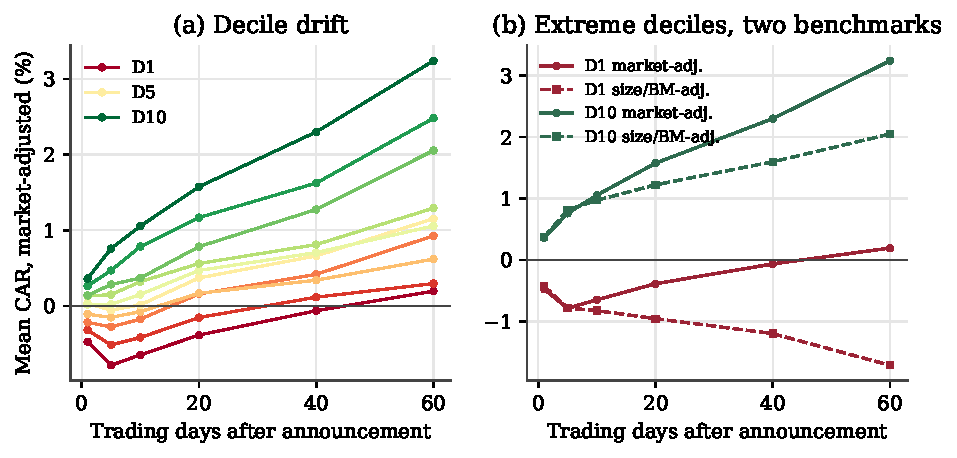
\includegraphics[width=\linewidth]{figures/fig_decile_drift.pdf}
\caption{(a) Mean market-adjusted cumulative return by SUE decile and horizon. (b) The extreme deciles
under the market benchmark (solid) and under the leave-one-out size/book-to-market benchmark
(dashed). Point-in-time deciles; recomputed from the corrected event file (Appendix~\ref{app:repro}).}\label{fig:decile}
\end{figure}

\begin{table}[t]\centering
\caption{Mean market-adjusted CAR (\%) by SUE decile and horizon (Fama--MacBeth means over \stv{Q} quarters).}\label{tab:deciles}
{\small
\begin{adjustbox}{max width=\linewidth}
\begin{tabular}{lrrrrrr}
\toprule
Decile & $+1$d & $+5$d & $+10$d & $+20$d & $+40$d & $+60$d \\
\midrule
D1 (most negative) & $-0.47$ & $-0.76$ & $-0.62$ & $-0.40$ & $-0.12$ & $+0.12$ \\
D2 & $-0.32$ & $-0.48$ & $-0.37$ & $-0.07$ & $+0.19$ & $+0.28$ \\
D3 & $-0.17$ & $-0.23$ & $-0.16$ & $+0.21$ & $+0.39$ & $+0.80$ \\
D4 & $-0.14$ & $-0.20$ & $-0.12$ & $+0.08$ & $+0.16$ & $+0.37$ \\
D5 & $-0.01$ & $-0.07$ & $+0.01$ & $+0.46$ & $+0.62$ & $+1.02$ \\
D6 & $+0.04$ & $+0.08$ & $+0.12$ & $+0.22$ & $+0.85$ & $+1.16$ \\
D7 & $+0.06$ & $+0.00$ & $+0.10$ & $+0.38$ & $+0.49$ & $+0.75$ \\
D8 & $+0.15$ & $+0.34$ & $+0.47$ & $+0.87$ & $+1.20$ & $+2.03$ \\
D9 & $+0.26$ & $+0.48$ & $+0.78$ & $+1.15$ & $+1.60$ & $+2.25$ \\
D10 (most positive) & $+0.33$ & $+0.66$ & $+0.96$ & $+1.44$ & $+2.12$ & $+3.02$ \\
\bottomrule
\end{tabular}
\end{adjustbox}
}

\end{table}

Table~\ref{tab:deciles} and Figure~\ref{fig:decile} show the canonical pattern. \stv{sent.monotone}
The top-minus-bottom spread \stv{sent.rising.mkt}, from \stv{spread.mkt.h1} at one day to
\stv{spread.mkt.h60} at 60 days (Table~\ref{tab:spreads}), and the smallest clustered
$t$-statistic across all horizons and both benchmarks is \stv{tmin_spread}. A one-time reaction that
merely differed across deciles would produce a flat spread; a rising spread is the signature of
gradual incorporation.

\paragraph{Effect of the point-in-time deciles on the signal.} Table~\ref{tab:pitcompare} compares the spreads under the earlier within-quarter ranking (\stv{pre.n_events} events, \stv{pre.Q} quarters) with the corrected ranking. The correction \stv{sent.pit_effect} the 60-day market-adjusted spread, from \stv{pre.spread.mkt.h60} to \stv{spread.mkt.h60}
(a difference of \stv{pit.drop60}); the signal itself survives the correction, and the larger cost of the correction is to the strategies built on the deciles (Section~\ref{sec:auditlog}).

\begin{table}[t]\centering
\caption{D10$-$D1 spread (\%) and quarter-clustered $t$-statistic under the earlier within-quarter ranking and under the corrected point-in-time ranking. Within-quarter columns: committed \texttt{data/} tables; point-in-time columns: corrected event file and \texttt{docs/paper/cache/pit/}.}\label{tab:pitcompare}
{\small
\begin{adjustbox}{max width=\linewidth}
\begin{tabular}{lrrrrrrrr}
\toprule
 & \multicolumn{2}{c}{Mkt-adj., within-quarter} & \multicolumn{2}{c}{Mkt-adj., point-in-time} & \multicolumn{2}{c}{Size/BM-adj., within-quarter} & \multicolumn{2}{c}{Size/BM-adj., point-in-time}\\
\cmidrule(lr){2-3}\cmidrule(lr){4-5}\cmidrule(lr){6-7}\cmidrule(lr){8-9}
Horizon & $\hat\mu$ & $t$ & $\hat\mu$ & $t$ & $\hat\mu$ & $t$ & $\hat\mu$ & $t$ \\
\midrule
$+1$d & 0.83 & 10.90 & 0.79 & 11.30 & 0.80 & 11.41 & 0.78 & 12.36 \\
$+5$d & 1.54 & 12.23 & 1.42 & 12.53 & 1.59 & 14.21 & 1.46 & 13.88 \\
$+10$d & 1.70 & 10.17 & 1.57 & 10.28 & 1.79 & 12.30 & 1.68 & 12.45 \\
$+20$d & 1.96 & 8.74 & 1.84 & 8.21 & 2.18 & 12.09 & 2.05 & 11.28 \\
$+40$d & 2.36 & 5.64 & 2.24 & 5.37 & 2.79 & 9.68 & 2.59 & 8.83 \\
$+60$d & 3.05 & 5.25 & 2.90 & 5.05 & 3.76 & 9.25 & 3.46 & 8.53 \\
\bottomrule
\end{tabular}
\end{adjustbox}
}

\end{table}

\paragraph{The shape of the drift.}
Fitting $\Delta(h)=a\,h^{b}$ to the six horizons gives $\Delta(h)\approx\stv{pl.ff.coef}\,h^{\stv{pl.ff.exp}}$
percent for the characteristic-adjusted spread ($R^2=\stv{pl.ff.r2log}$ in logs) and
$\stv{pl.mkt.coef}\,h^{\stv{pl.mkt.exp}}$ for the market-adjusted spread ($R^2=\stv{pl.mkt.r2log}$).
A single-speed saturating exponential, $A(1-e^{-h/\tau})$, \stv{sent.expfit} on the same points
($R^2=\stv{pl.ff.exp_r2}$ and $\stv{pl.mkt.exp_r2}$ in levels, against \stv{pl.ff.r2lvl} and
\stv{pl.mkt.r2lvl} for the power law). Growth that is a power of the horizon and has not saturated
by day 60 is consistent with the heterogeneous-attention mixture \eqref{eq:phi}, in which the
unincorporated fraction decays as a power and there is no single time scale. With only six
horizons the evidence is suggestive, not a test between the two functional forms.

\subsection{Is the drift a risk premium in disguise?}\label{sec:riskprem}

Extreme-bad-news firms tend to be small, high book-to-market firms that earn a size and value
premium. In market-adjusted terms \stv{sent.d1recovery}, which raises the possibility that part of
the drift is compensation for risk rather than mispricing. We test this with a characteristic
benchmark in the spirit of \citet{DGTW1997}. Each event is assigned to a cell $c(i)$ defined by
quarter, size quintile, and book-to-market tercile, and its return is measured against the average of
its cell-mates, excluding itself:
\begin{equation}
  \widetilde{\mathrm{CAR}}_i(h)=\mathrm{CAR}_i(h)-\frac{\sum_{j\in c(i)}\mathrm{CAR}_j(h)-\mathrm{CAR}_i(h)}{n_{c(i)}-1}.
  \label{eq:loo}
\end{equation}
Leaving the event out of its own benchmark prevents its return from shrinking toward zero in thin
cells. If the drift were a risk premium, the adjustment would shrink the spread. It \stv{sent.ffvsmkt}
it: the 60-day spread moves from \stv{spread.mkt.h60} to \stv{spread.ff.h60}
($t=\stv{spread.ff.t.h60}$), and the worst decile \stv{sent.d1ff}. The apparent reversal of the worst decile was a
size/value premium sitting on top of the drift (Table~\ref{tab:spreads}, Figure~\ref{fig:spreads}).

\begin{table}[t]\centering
\caption{Top-minus-bottom decile spread by horizon (\%), with quarter-clustered $t$-statistics.
Equity columns use the full sample with point-in-time deciles. Option columns are from the pre-correction option tables (within-quarter deciles): they use the option-matched subsample
(\stv{Q_opt} quarters; \stv{Q_opt60} at $+60$d) and measure the percentage return on premium of a
buy-and-hold near-the-money contract at its mid price.}\label{tab:spreads}
{\small
\begin{adjustbox}{max width=\linewidth}
\begin{tabular}{lrrrrrrrrrr}
\toprule
 & \multicolumn{2}{c}{Mkt-adj.\ equity} & \multicolumn{2}{c}{Size/BM-adj.\ equity} & \multicolumn{2}{c}{Call} & \multicolumn{2}{c}{Put} & \multicolumn{2}{c}{Straddle}\\
\cmidrule(lr){2-3}\cmidrule(lr){4-5}\cmidrule(lr){6-7}\cmidrule(lr){8-9}\cmidrule(lr){10-11}
Horizon & $\hat\mu$ & $t$ & $\hat\mu$ & $t$ & $\hat\mu$ & $t$ & $\hat\mu$ & $t$ & $\hat\mu$ & $t$ \\
\midrule
$+1$d & 0.79 & 11.30 & 0.78 & 12.36 & 4.01 & 13.33 & $-$2.49 & $-$13.21 & 0.27 & 3.31 \\
$+5$d & 1.42 & 12.53 & 1.46 & 13.88 & 8.03 & 13.27 & $-$5.11 & $-$13.04 & 0.77 & 4.61 \\
$+10$d & 1.57 & 10.28 & 1.68 & 12.45 & 9.54 & 11.87 & $-$5.86 & $-$13.01 & 1.24 & 4.87 \\
$+20$d & 1.84 & 8.21 & 2.05 & 11.28 & 11.29 & 8.34 & $-$6.46 & $-$7.91 & 2.18 & 4.97 \\
$+40$d & 2.24 & 5.37 & 2.59 & 8.83 & 11.76 & 5.67 & $-$8.27 & $-$6.64 & 2.80 & 5.10 \\
$+60$d & 2.90 & 5.05 & 3.46 & 8.53 & 14.38 & 4.69 & $-$10.79 & $-$6.29 & 3.98 & 5.22 \\
\bottomrule
\end{tabular}
\end{adjustbox}
}

\end{table}

\subsection{The cross-section of the drift}

If frictions sustain the drift, it should differ across stocks in a predictable way. We compute the
60-day quarterly spread separately within each group and test equality of group means with a
Cochran $Q$ statistic built from the group estimates and their standard errors. This treats groups as
independent, which they are not exactly (they share quarters), so the $p$-values are approximate.
The one-way ANOVA on the raw spread series reported in earlier drafts needs the series themselves, which are not
among the saved files; we therefore do not quote it.
\begin{itemize}
  \item \textbf{Industry (Fama--French 12).} The spread is \stv{sent.het_sector}: the group estimates
        run from \stv{sector.min} (\stv{sector.min.name}) to \stv{sector.max}
        (\stv{sector.max.name}) across \stv{sector.n} groups ($Q=\stv{het.sector.Q}$, $p=\stv{het.sector.p}$).
        One drift model is therefore used for the whole cross-section.
  \item \textbf{Size.} The heterogeneity is \stv{sent.het_size}. The spread \stv{sent.sizemono} with
        size, from \stv{size.small} ($t=\stv{size.small.t}$) in the smallest quintile to
        \stv{size.large} ($t=\stv{size.large.t}$) in the largest. This is the prediction of
        Section~\ref{sec:mechanism}: the drift is greatest where arbitrage is most expensive. Size is a
        first-order determinant of the signal's value, so a strategy must neutralize it, not simply load on it.
  \item \textbf{Era.} The estimates run from \stv{era.first} (\stv{era.first.name}) to \stv{era.last}
        (\stv{era.last.name}). \stv{sent.het_era}.
\end{itemize}

\begin{figure}[t]\centering
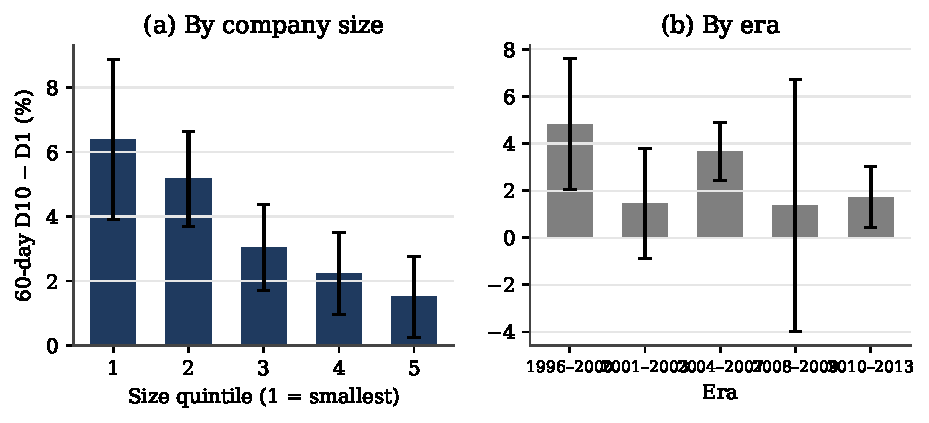
\includegraphics[width=\linewidth]{figures/fig_heterogeneity.pdf}
\caption{60-day D10$-$D1 spread with 95\% confidence intervals by (a) size quintile at announcement
and (b) era. Point-in-time deciles, recomputed from the corrected event file (Appendix~\ref{app:repro}).}\label{fig:het}
\end{figure}
\begin{table}[t]\centering
\caption{The 60-day spread by size quintile and by era.}\label{tab:het}
{\small
\begin{adjustbox}{max width=\linewidth}
\begin{tabular}{lrrr}
\toprule
Group & 60d D10$-$D1 (\%) & $t$ & Events \\
\midrule
Size quintile 1 (smallest) & 6.39 & 5.06 & 20{,}574 \\
Size quintile 2 & 5.17 & 6.83 & 33{,}305 \\
Size quintile 3 & 3.05 & 4.47 & 37{,}966 \\
Size quintile 4 & 2.24 & 3.45 & 41{,}331 \\
Size quintile 5 (largest) & 1.51 & 2.37 & 45{,}374 \\
\midrule
Era 1996--2000 & 4.82 & 3.40 & 43{,}884 \\
Era 2001--2003 & 1.45 & 1.21 & 26{,}346 \\
Era 2004--2007 & 3.66 & 5.79 & 41{,}953 \\
Era 2008--2009 & 1.37 & 0.50 & 22{,}308 \\
Era 2010--2013 & 1.72 & 2.59 & 44{,}062 \\
\bottomrule
\end{tabular}
\end{adjustbox}
}

\end{table}

\subsection{Rival hypotheses that were tested and rejected}\label{sec:rivals}

\paragraph{Surprise reversal.} \citet{BernardThomas1990} report a lag-four-quarter SUE
autocorrelation of about \stv{rev.lit}. On \stv{rev.n} firm pairs we estimate \stv{rev.ac}. Firms in the
top decile four quarters earlier still average a standardized surprise of \stv{rev.d10} against \stv{rev.d1} for the
bottom decile. The data show persistence, not reversal, so no book fades a firm's own past surprise.

\paragraph{Announcement-return (EAR) augmentation.} Blending the day-0 return into the signal leaves
the Sharpe ratio flat (\stv{ear.range} across blend weights, as recorded in \texttt{docs/HISTORY.md}).
That holds once the EAR input is restricted to information realized before the first accrual day. An
earlier specification used the day-0-to-day-1 return, which overlaps a position's first day of P\&L,
and it produced a spurious Sharpe ratio that kept rising with the blend weight (Section~\ref{sec:audit}).
The machine-readable output of this diagnostic is not kept in \texttt{results/}, so these two statements rest on the
project history, not on a file the build reads.

\paragraph{Filtering by volatility.} Volatility does not change average returns; it changes how much
a given surprise is worth (Section~\ref{sec:calm}). Walk-forward filters that drop whole volatility groups \stv{sent.filter_vs_sizing} sizing on the Sharpe ratio
(Section~\ref{sec:calm}); the negative result is kept as \sn{volatility_filter} and
\sn{calm_weighted_filter}.

\subsection{The signal in option premia (mid prices, pre-correction deciles)}

If PEAD is a real mispricing of the stock, it should appear in the price of a leveraged claim on that
stock. This section measures the signal in option premia at mid prices and with the earlier within-quarter deciles (the option tables were not rebuilt); it says nothing about what an option trader pays, which Section~\ref{sec:options} measures. For each event with listed options we take, on the announcement day, the call (put) with delta
nearest $+0.5$ ($-0.5$) and at least 95 calendar days to expiry. We hold it at its mid price to each
horizon. The call spread is $+$\stv{call60} of premium at 60 days ($t=\stv{call60.t}$) and the put
spread is \stv{put60} ($t=\stv{put60.t}$), the mirror image (Table~\ref{tab:spreads},
Figure~\ref{fig:spreads}).

\paragraph{Magnitude check.} The ratio of the 60-day call spread to the stock spread is
$\stv{call60}/\stv{spread.mkt.h60}\approx\stv{amp_ratio}$. This is \stv{sent.ampband} the
elasticity band $\Omega\in[\stv{omega_lo},\stv{omega_hi}]$ from equation~\eqref{eq:omega}. These are returns on premium between mid prices, before the bid/ask spread.

\paragraph{Direction versus volatility.} A long straddle has roughly zero delta and isolates the
non-directional component. Its 60-day spread is $+$\stv{str60} ($t=\stv{str60.t}$), a fraction
\stv{str_over_call} of the call spread. Extreme-surprise names carry some excess volatility, but the
dominant effect is directional.

\begin{figure}[t]\centering
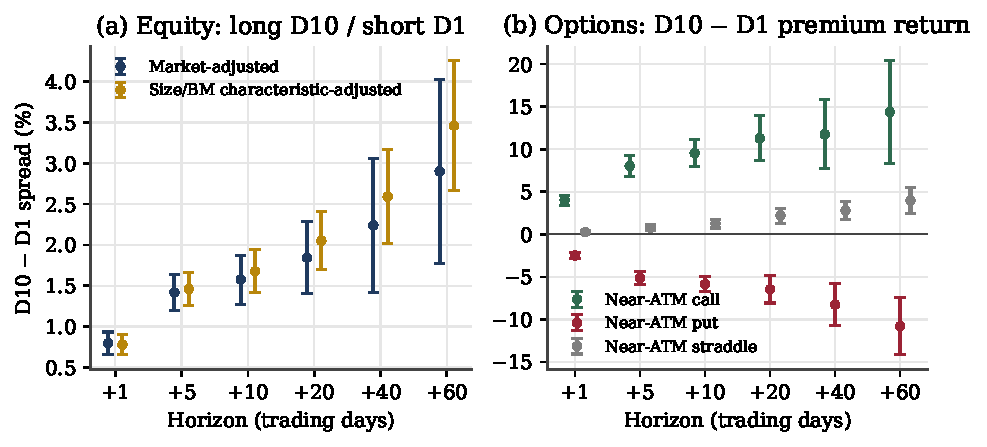
\includegraphics[width=\linewidth]{figures/fig_spreads.pdf}
\caption{D10$-$D1 spreads with 95\% quarter-clustered confidence intervals. (a) Equity, market-adjusted and
characteristic-adjusted. (b) Near-the-money options, as return on premium.}\label{fig:spreads}
\end{figure}

\subsection{When to stop holding: the decay of the drift}\label{sec:decay}

A trading rule must decide when the marginal day of holding stops paying. Let $a(H)$ be the expected
abnormal return from holding a position for $H$ days, net of the entry and exit cost $k$. When capital is
recycled into the next opportunity, the quantity to maximize is the average net return per capital-day,
\begin{equation}
  \mathcal Y(H)=\frac{a(H)-k}{H},\qquad a(H)=\lambda|z|\big[\phi(H)-\phi(0)\big].
  \label{eq:holding}
\end{equation}
The first-order condition is $a'(H^\ast)=\mathcal Y(H^\ast)$: hold until the marginal daily drift falls to
the average daily net yield. Because $\phi$ is concave, $a'$ is decreasing, and $H^\ast$ is unique whenever
the total drift exceeds the cost (Appendix~\ref{app:proofs}). Higher trading costs lengthen $H^\ast$.

The empirical analogue estimates a holding window for each cell of (decile $\times$ size quintile
$\times$ book-to-market tercile). Let $\overline{\mathrm{CAR}}_c(d)$ be the mean characteristic-adjusted
cumulative return of cell $c$ on holding day $d$. A trailing windowed slope
$\varsigma_c(d)=\big[\overline{\mathrm{CAR}}_c(d)-\overline{\mathrm{CAR}}_c(d-W)\big]/W$ with
$W=\stv{decay.window}$ is compared with a cell-specific threshold of \stv{decay.thresh} of its own early
peak, $\theta_c$. The decay day $H_c$ is the first day after a \stv{decay.burn_in}-day burn-in on which
$|\varsigma_c|<\theta_c$ or the slope has changed sign, and stays that way for \stv{decay.persist} consecutive days.
A cell with too little history backs off to (decile $\times$ size), then to the decile alone;
\stv{decay.fine} of the \stv{decay.n} estimated cells are the finest cells. Across cells $H_c$ ranges from
\stv{decay.min} to \stv{decay.max} trading days (median \stv{decay.median}, mean \stv{decay.mean}); the mean is
\stv{decay.d1} for D1 and \stv{decay.d10} for D10, against \stv{decay.d6} for D6 near the median.
The windows are now estimated on the first \stv{fix.decay.pct} of announcement quarters (\stv{fix.decay.n} of \stv{fix.decay.of}) and applied to every event; earlier drafts fitted them on the whole sample,
which used information a live trader would not have (Section~\ref{sec:auditlog}). The back-off thresholds for thin cells and the leave-one-out risk benchmark of Section~\ref{sec:riskprem} still see the full sample.

%=====================================================================================
\section{The equity strategy family}\label{sec:equity}
%=====================================================================================

\subsection{From signal to portfolio}

A book goes long positive surprises and short negative ones, with size increasing in the strength of
the surprise, and it holds each position for the decay time of Section~\ref{sec:decay}. Write
$\delta_i=u_i-\tfrac12\in(-\tfrac12,\tfrac12]$ for the centered within-quarter rank. All the neutralized
books share one weight construction.

\begin{definition}[Trimmed, tilted, neutralized weights]\label{def:weights}
For a trim $\tau$, a tilt $\gamma$ and a per-event scale $s_i>0$ (identically one unless a book sizes by
volatility), define the conviction
$t_i=\1\{|\delta_i|>\tau\}\,\sgn(\delta_i)\,(2|\delta_i|)^{\gamma}\,s_i$. For quarter $q$ and side
$\sigma\in\{+,-\}$ let $\mathcal{G}_{q\sigma}$ be the set of occupied groups, where a group is a pair
(industry, size quintile), and $N_{q\sigma}=|\mathcal G_{q\sigma}|$. The weights are
\begin{equation}
  \tilde w_i=\frac{t_i}{\sum_{j\in g(i)}|t_j|}\cdot\frac{1}{N_{q\sigma}},\qquad
  w_i=\frac{\tilde w_i}{2\,\overline{|\tilde w|}},
  \label{eq:weights}
\end{equation}
where $\overline{|\tilde w|}$ is a global normalizing constant.
\end{definition}

Within a group the weight is proportional to conviction, and each group receives the same total
weight on each side. The construction targets the unpriced risks the evidence identified: industry
concentration and size, the dimension along which the drift itself varies. In the code, $\tau=\stv{balanced_leverage.trim}$ and
$\gamma=\stv{balanced_leverage.tilt}$ for the books built on \sn{balanced_leverage}; $s_i=1/\mathrm{ivol}_i$
(idiosyncratic volatility, clipped) for \sn{calm_weighted}, and $s_i=(1.02-\pi_i)^{k}$ with $\pi_i$ the
volatility percentile against the previous quarter's cross-section within the stock's size quintile and
$k=\stv{calm_rank_tilt.power}$ for \sn{calm_rank_tilt}.

\begin{proposition}[Neutrality]\label{prop:neutral}
For every quarter's entry cohort, before any capacity cap:
(a) the long and short sides have equal gross weight, so the cohort is dollar-neutral;
(b) each occupied (industry, size) group receives exactly $1/N_{q\sigma}$ of its side's gross;
(c) net exposure to industry $k$ equals $\big(n^{+}_{k}/N_{q+}-n^{-}_{k}/N_{q-}\big)$ times the global
constant, where $n^\sigma_k$ is the number of occupied size buckets of industry $k$ on side $\sigma$. It
vanishes whenever both sides occupy the same groups, and the same holds for size.
\end{proposition}

\subsection{Engine, sizing and costs}\label{sec:engine}

One engine runs every equity book. Position $i$ has dollar notional $n_i=w_i\,b\,V_q$, with $V_q$ the
previous quarter-end NAV (so profits affect sizing only from the next quarter) and $b$ the base-unit
fraction. The notional is capped at a fraction ($\stv{balanced_leverage.liqfrac}$ of the stock's 21-day average dollar volume), and the
gross exposure of the whole open book is capped at a multiple of the NAV on which the quarter is sized, with new positions trimmed (lowest conviction first) to fit the room left on every day they will be held. Round-trip costs are $\stv{cost.bps}$ basis points by liquidity
quintile (thinnest to most liquid), charged at entry and at exit. Because returns are measured against
the market, each stock position is economically paired with an offsetting index position, and the daily
P\&L is
\begin{equation}
  \Pi_t=\sum_{i\ \text{open at }t}n_i\,(r_{i,t}-r_{m,t})\;-\;\sum_{i\ \text{entering or exiting at }t}|n_i|\,k_i,
  \label{eq:pnl}
\end{equation}
with $k_i$ the liquidity-dependent cost. The exceptions are \sn{market_exposed}, which uses raw returns
on purpose, and the books with a market overlay (\sn{market_boost}), which add a separate market
position. Combining \eqref{eq:drift} with the weights, the expected P\&L of one cohort is
$\E[\Pi]=\lambda bV\sum_i w_i z_i[\phi(H_i)-\phi(0)]-\text{costs}$, the covariance between conviction and
drift. Since the book is balanced across industries and size by Proposition~\ref{prop:neutral}, the sum does
not rely on any industry or size effect, only on the within-group ordering of surprises.

Two features of the engine matter for how the results are read. First, the cap holds at sizing time, but positions are fixed in dollars, so gross exposure divided by the \emph{current} NAV can still exceed it when NAV falls: for \sn{calm_weighted}, whose cap is
\stv{calm_weighted.cap}$\times$, realized gross exposure divided by NAV averages \stv{calm_weighted.gross_avg}$\times$,
exceeds the cap on \stv{calm_weighted.days_over_cap} of days and peaks at \stv{calm_weighted.gross_max}$\times$ (before the correction, which counted only each quarter's new positions: \stv{calm_weighted_legacy.days_over_cap} of days and a peak of \stv{calm_weighted_legacy.gross_max}$\times$; Section~\ref{sec:auditlog}). Second, summary statistics in \texttt{results/} are computed over the full calendar,
including the idle period before the first position (the equity books start trading in
\stv{calm_weighted.active_start}; the options books in \stv{options_cap20.active_start}). Active-period Sharpe ratios differ from the stored ones (for example \stv{calm_weighted.sharpe_active} against
\ssh{calm_weighted} for \sn{calm_weighted}), and Table~\ref{tab:dsr} uses active-period returns.

\paragraph{Breadth.} The book opens about \stv{calm_weighted.pos_per_year} positions a year. The fundamental law of active management
\citep{Grinold1989}, $\mathrm{IR}\approx\mathrm{IC}\sqrt{\mathrm{BR}}$, with $\mathrm{BR}$ the number of independent bets, then
implies a per-bet information coefficient of about \stv{calm_weighted.implied_ic} if every position were an independent bet (they are
not, so the implied coefficient is a lower bound on the true one). The equity book is a breadth strategy: many weak bets rather than a
few strong ones. Its volatility comes from the residual common factors that neutrality does not remove.

\subsection{The family}\label{sec:family}

Table~\ref{tab:family} lists the family in lineage order, with each book's plain description from its own metadata. The progression
follows the diagnoses recorded in the repository: \sn{extreme_picks} is the textbook trade; \sn{graded_bets} and \sn{size_balanced} change the
weights; \sn{conviction_tilt} trims the middle of the ranking, tilts toward the extremes and drops the lowest-conviction positions first when a cap binds;
\sn{sector_balanced} adds industry neutrality; \sn{balanced_leverage} raises the gross cap; \sn{market_boost} and \sn{market_exposed} add market exposure
deliberately (the first) or by accident (the second); the \sn{calm_*} books size by volatility.

\begin{table}[t]\centering
\caption{The equity family in lineage order. ``Unit / cap'' is the base-unit fraction and the gross-exposure cap
(open book, at sizing time). Returns, Sharpe ratios and drawdowns are from \texttt{results/<name>/summary.json}.}\label{tab:family}
{\footnotesize
\begin{tabularx}{\linewidth}{@{}l l X l r r r@{}}
\toprule
Book & Status & What it does & Unit / cap & Return & Sharpe & Max DD\\
\midrule
\sn{extreme_picks} & validated & Buy the top 10\% of earnings surprises, short the bottom 10\%, equal bets & 0.003 / 1.5$\times$ & 3.3\% & 0.65 & $-$25.2\% \\
\sn{graded_bets} & validated & Bet on every stock; the more extreme the surprise, the bigger the bet & 0.002 / 1.5$\times$ & 2.4\% & 0.62 & $-$19.5\% \\
\sn{size_balanced} & validated & Extreme Picks, with an equal budget for each of the five company sizes & 0.003 / 1.5$\times$ & 3.8\% & 0.81 & $-$18.1\% \\
\sn{conviction_tilt} & validated & Skip the middle 15\% either side of average, lean toward the strongest surprises, balance by size & 0.002 / 1.5$\times$ & 3.8\% & 0.97 & $-$14.5\% \\
\sn{sector_balanced} & validated & Conviction Tilt, also balanced across 12 industry groups; conservative 1.5x borrowing limit & 0.0015 / 1.5$\times$ & 3.1\% & 1.08 & $-$11.4\% \\
\sn{balanced_leverage} & validated & Sector Balanced, allowed to hold up to 2.5x the account in positions & 0.003 / 2.5$\times$ & 5.4\% & 1.09 & $-$18.6\% \\
\sn{market_boost} & validated & Balanced Leverage plus a market position worth half the account & 0.003 / 2.5$\times$ & 9.2\% & 0.90 & $-$25.1\% \\
\sn{market_exposed} & reference & Balanced Leverage signal, longs and shorts not forced to match, market moves left in & 0.003 / 2.5$\times$ & 6.6\% & 0.72 & $-$34.1\% \\
\sn{calm_weighted} & validated & Balanced Leverage, with each bet divided by how jumpy the stock is & 0.003 / 2.5$\times$ & 5.6\% & 1.24 & $-$17.5\% \\
\sn{calm_weighted_matched} & validated & Calm Weighted resized so its ups and downs match Balanced Leverage exactly (4.94\% a year) & 0.00346881 / 2.5$\times$ & 5.8\% & 1.18 & $-$18.7\% \\
\sn{volatility_filter} & research & Balanced Leverage, skipping long/short x jumpiness groups that have not made money so far & 0.003 / 2.5$\times$ & 4.6\% & 0.89 & $-$18.8\% \\
\sn{calm_weighted_filter} & research & Calm Weighted plus the Volatility Filter & 0.003 / 2.5$\times$ & 5.1\% & 1.08 & $-$17.6\% \\
\sn{calm_rank_tilt} & research & Balanced Leverage, with bets shrunk sharply for the jumpiest stocks (ranked against last quarter) & 0.003 / 2.5$\times$ & 6.0\% & 1.47 & $-$13.6\% \\
\sn{calm_rank_levered} & research & Calm Rank Tilt with its lower risk spent on larger bets (about 1.7x) and a 4x borrowing limit & 0.005 / 4$\times$ & 8.1\% & 1.39 & $-$19.6\% \\
\bottomrule
\end{tabularx}
}

\end{table}

\subsection{Headline results}\label{sec:eqresults}

\begin{table}[t]\centering
\caption{Equity headline books, 1996--2013 (net of modeled costs; borrow and financing not modeled).}\label{tab:eqheadline}
{\small
\begin{adjustbox}{max width=\linewidth}
\begin{tabular}{lrrrrrl}
\toprule
Book & Return & Vol & Sharpe & Max DD & Calmar & Role \\
\midrule
\sn{calm_weighted} & 6.71\% & 4.49\% & 1.47 & $-$15.6\% & 0.43 & validated headline \\
\sn{calm_rank_tilt} & 7.12\% & 3.83\% & 1.81 & $-$11.6\% & 0.61 & research headline \\
\sn{balanced_leverage} & 6.49\% & 4.94\% & 1.30 & $-$16.6\% & 0.39 & reference \\
\sn{market_exposed} & 7.30\% & 6.56\% & 1.11 & $-$15.5\% & 0.47 & reference \\
\sn{market_boost} & 10.08\% & 10.51\% & 0.97 & $-$23.2\% & 0.43 & validated \\
\bottomrule
\end{tabular}
\end{adjustbox}
}

\end{table}

\paragraph{The validated book.} \sn{calm_weighted} divides each bet by the stock's idiosyncratic volatility. It has no fitted parameter beyond the
construction shared with \sn{balanced_leverage}. It earns \sret{calm_weighted} a year at \svol{calm_weighted} volatility (Sharpe \ssh{calm_weighted}, maximum
drawdown \sdd{calm_weighted}, Calmar \stv{calm_weighted.calmar}), compared with \sret{balanced_leverage} and a Sharpe ratio of \ssh{balanced_leverage} for
\sn{balanced_leverage}. It has a higher Sharpe ratio than \sn{balanced_leverage} in \stv{calm_vs_bl.n_better} of the three sub-periods
(\stv{calm_weighted.shA}, \stv{calm_weighted.shB}, \stv{calm_weighted.shC} against \stv{balanced_leverage.shA}, \stv{balanced_leverage.shB},
\stv{balanced_leverage.shC}). Before the corrections it earned \stv{calm_weighted_legacy.ret} at a Sharpe ratio of \stv{calm_weighted_legacy.sharpe}; the corrected return is \stv{sent.eq_fix_dir}. Its return is \stv{sent.cw_vs_mkt} that of the CRSP market (\stv{market.ret} a year at \stv{market.vol} volatility, Sharpe
\stv{market.sharpe}, worst drawdown \stv{market.dd}, over the same calendar, \stv{market.window}): the book is market-neutral, and is not designed to beat the index.

\paragraph{The research book.} \sn{calm_rank_tilt} weights each event by $(1.02-\pi_i)^k$, which all but switches off the most volatile stocks. Its Sharpe ratio
\stv{sent.calmprogress} along the lineage \sn{balanced_leverage} ($\ssh{balanced_leverage}$), \sn{calm_weighted} ($\ssh{calm_weighted}$), \sn{calm_rank_tilt}
($\ssh{calm_rank_tilt}$), and it is higher than \sn{calm_weighted}'s in \stv{crt_vs_cw.n_better} of the three sub-periods. \textbf{It is a research book, not a
validated one:} the exponent $k=\stv{calm_rank_tilt.power}$ was chosen after seeing \sn{calm_weighted}'s full-sample results, so its Sharpe ratio is
in-sample. The only out-of-sample evidence is a split-sample check recorded with the strategy: an exponent chosen on \stv{split.train} data alone (best
$k=\stv{split.k}$) lifts the \stv{split.test} Sharpe ratio from \stv{split.from} to \stv{split.to}, the same as the full-sample best. That is one check on
one split, and it predates the corrections and was not re-run. It supports the direction of the tilt, not the level of the Sharpe ratio. Before the corrections the book earned \stv{calm_rank_tilt_legacy.ret} at a Sharpe ratio of \stv{calm_rank_tilt_legacy.sharpe}.

\paragraph{The reference and the cautionary books.} \sn{balanced_leverage} is the pure-alpha reference. \sn{market_exposed} uses raw returns and lets net exposure float;
its net dollar exposure is only \stv{market_exposed.net_to_gross} of gross yet its beta against the market is \stv{market_exposed.beta} (alpha \stv{market_exposed.alpha}),
because equal dollars long and short are not equal beta. \sn{market_boost} adds a market position of \stv{market_boost.overlay} times NAV to \sn{balanced_leverage}: return \sret{market_boost},
volatility \svol{market_boost}, beta \stv{market_boost.beta}. It earns the market's premium on top of the alpha and carries the market's drawdown (\sdd{market_boost}). Its return \stv{sent.mb_clears} the market's \stv{market.ret} over the same calendar.

\subsection{The leveraged and market-exposed research variants}\label{sec:levered}

Earlier drafts headlined an equity book earning \stv{olddraft.eq.ret} at \stv{olddraft.eq.vol} volatility (Sharpe \stv{olddraft.eq.sharpe},
drawdown \stv{olddraft.eq.dd}). That book is \stv{olddraft.eq.name}, the pre-correction run of the six-times-cap research variant; it was never the validated headline. Corrected, \sn{balanced_leverage_max} earns \sret{balanced_leverage_max} (Sharpe \ssh{balanced_leverage_max}, drawdown \sdd{balanced_leverage_max}), and it is \stv{oldhead.same} to \sn{sector_balanced_max}. Each \sn{*_max} book keeps its parent's signal and neutralization and changes only two dials, the base unit and a gross cap of
\stv{balanced_leverage_max.cap}$\times$. The base unit was chosen by sweeping the unit and taking the highest return subject to a Sharpe ratio of at least \stv{rule.sharpe} and a drawdown no
worse than $-$\stv{rule.dd} (Section~\ref{sec:capacity}): an in-sample choice, not re-made after the corrections, and \stv{max.n_breach} of the \stv{max.n} \sn{*_max} books now breach that drawdown limit (worst: \stv{max.worst_dd}). Table~\ref{tab:levered} reports them with the leverage they actually use. Realized gross
exposure for \sn{balanced_leverage_max} averages \stv{balanced_leverage_max.gross_avg}$\times$ NAV and peaks at \stv{balanced_leverage_max.gross_max}$\times$, which is
prime-brokerage-level leverage, and \stv{balanced_leverage_max.liqcap} of its positions sit at the volume cap. Its return is \stv{sent.levered_ret} and its Sharpe ratio is
\stv{sent.levered_sh} than \sn{calm_weighted}'s, with a \stv{sent.levered_dd} drawdown. \sn{market_boost_max} adds the market overlay to this book: it earns
\sret{market_boost_max} (Sharpe \ssh{market_boost_max}), which is \stv{sent.mbmax_vs_mkt} the market's \stv{market.ret}, a beta of \stv{market_boost_max.beta} and a drawdown of \sdd{market_boost_max}. The
extra return is the market's, paid for with the market's drawdown, and it should be read as a leveraged, market-exposed research variant.

\begin{table}[t]\centering
\caption{Leveraged and market-exposed research variants (top block) with the unlevered books for comparison (bottom block). Average and maximum gross exposure divided
by NAV are measured on days with positions, from \texttt{daily.csv.gz}; ADV-capped is the share of positions at the \stv{balanced_leverage.liqfrac} volume cap.}\label{tab:levered}
{\small
\begin{adjustbox}{max width=\linewidth}
\begin{tabular}{lrrrrrrrr}
\toprule
Book & Return & Vol & Sharpe & Max DD & Avg gross & Max gross & ADV-capped & Beta \\
\midrule
\sn{market_boost_max} & 11.6\% & 14.0\% & 0.86 & $-$44.6\% & 3.5$\times$ & 6.6$\times$ & 49\% & 0.49 \\
\sn{conviction_tilt_max} & 9.3\% & 12.6\% & 0.76 & $-$40.5\% & 3.7$\times$ & 6.9$\times$ & 29\% & 0.03 \\
\sn{size_balanced_max} & 8.9\% & 13.0\% & 0.72 & $-$43.6\% & 2.9$\times$ & 5.6$\times$ & 46\% & 0.03 \\
\sn{market_exposed_max} & 11.5\% & 17.2\% & 0.72 & $-$53.8\% & 2.9$\times$ & 5.8$\times$ & 27\% & 0.51 \\
\sn{balanced_leverage_max} & 8.3\% & 12.8\% & 0.69 & $-$44.9\% & 4.6$\times$ & 7.6$\times$ & 49\% & $-$0.02 \\
\sn{sector_balanced_max} & 8.3\% & 12.8\% & 0.69 & $-$44.9\% & 4.6$\times$ & 7.6$\times$ & 49\% & $-$0.02 \\
\sn{graded_bets_max} & 8.6\% & 14.4\% & 0.64 & $-$48.0\% & 4.3$\times$ & 8.4$\times$ & 59\% & 0.02 \\
\sn{extreme_picks_max} & 9.0\% & 15.6\% & 0.63 & $-$56.4\% & 3.2$\times$ & 7.4$\times$ & 51\% & 0.05 \\
\midrule
\sn{balanced_leverage} & 5.4\% & 4.9\% & 1.09 & $-$18.6\% & 1.8$\times$ & 2.7$\times$ & 15\% & $-$0.00 \\
\sn{calm_weighted} & 5.6\% & 4.5\% & 1.24 & $-$17.5\% & 1.8$\times$ & 2.7$\times$ & 15\% & $-$0.01 \\
\sn{calm_rank_tilt} & 6.0\% & 4.0\% & 1.47 & $-$13.6\% & 1.7$\times$ & 2.6$\times$ & 14\% & $-$0.02 \\
\sn{calm_rank_levered} & 8.1\% & 5.7\% & 1.39 & $-$19.6\% & 2.4$\times$ & 4.1$\times$ & 18\% & $-$0.03 \\
\sn{market_boost} & 9.2\% & 10.4\% & 0.90 & $-$25.1\% & 1.2$\times$ & 2.0$\times$ & 15\% & 0.51 \\
\bottomrule
\end{tabular}
\end{adjustbox}
}

\end{table}

\begin{figure}[t]\centering
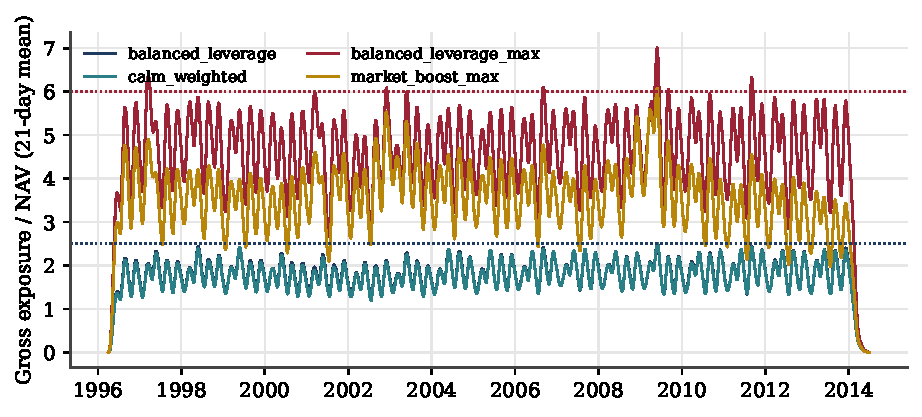
\includegraphics[width=\linewidth]{figures/fig_leverage.pdf}
\caption{Realized gross exposure divided by NAV (21-day mean). Dotted lines mark the nominal caps. The cap holds at sizing time; gross over current NAV can exceed it when NAV falls.}\label{fig:leverage}
\end{figure}

%=====================================================================================
\section{Where the equity return comes from}\label{sec:where}
%=====================================================================================

\begin{sloppypar}This section decomposes the equity returns. It rests on the saved attribution files (\texttt{results/alpha\_benchmark.csv}, \texttt{situations\_*.csv}, \texttt{profiles\_*.csv}), which
split every position's profit into a part that the surprise rank predicts (``alpha'') and a part that comes from holding the average announcer.\end{sloppypar}

\subsection{Alpha against the market}\label{sec:alpha}

Daily NAV-percentage returns are regressed on the CRSP value-weighted market return (zero risk-free rate, Newey--West standard errors with five lags), alone and with an equal-weight-minus-value-weight
(size) factor. Table~\ref{tab:alpha} reports the results. Across the \stv{beta.neutral.n} market-neutral books the largest absolute beta is \stv{beta.neutral.maxabs}; the market-exposed
books (\sn{market_exposed}, \sn{market_boost} and their \sn{*_max} versions) carry betas between \stv{beta.exposed.min} and \stv{beta.exposed.max}. For \sn{calm_weighted} the alpha is \stv{calm_weighted.alpha}
($t=\stv{calm_weighted.alpha_t}$); adding the size factor changes it to \stv{calm_weighted.alpha_sz}. \stv{sent.alphafade}.

\begin{table}[t]\centering
\caption{Annualized alpha against the CRSP value-weighted market, with and without a size factor, by era. $t$-statistics use Newey--West errors; IR is alpha over
residual volatility. Source: \texttt{results/alpha\_benchmark.csv}.}\label{tab:alpha}
{\small
\begin{adjustbox}{max width=\linewidth}
\begin{tabular}{lrrrrrrrrrr}
\toprule
Book & Return & Alpha & $t$ & Beta & Alpha (+size) & $t$ & IR & 96--01 & 02--07 & 08--13 \\
\midrule
\sn{calm_rank_tilt} & 6.0\% & 6.5\% & 6.4 & $-$0.02 & 6.4\% & 6.3 & 1.57 & 11.4\% & 6.6\% & 2.2\% \\
\sn{calm_weighted} & 5.6\% & 6.1\% & 5.2 & $-$0.01 & 6.4\% & 5.6 & 1.31 & 10.2\% & 6.8\% & 1.6\% \\
\sn{balanced_leverage} & 5.4\% & 5.8\% & 4.5 & $-$0.00 & 6.2\% & 4.9 & 1.14 & 9.4\% & 6.9\% & 1.3\% \\
\sn{conviction_tilt} & 3.8\% & 4.0\% & 3.9 & 0.01 & 4.3\% & 4.2 & 0.98 & 5.4\% & 4.4\% & 1.8\% \\
\sn{sector_balanced} & 3.1\% & 3.4\% & 4.5 & $-$0.00 & 3.5\% & 4.9 & 1.12 & 5.3\% & 3.6\% & 1.3\% \\
\sn{extreme_picks} & 3.3\% & 3.7\% & 2.9 & $-$0.01 & 4.4\% & 3.6 & 0.69 & 4.4\% & 6.3\% & 0.0\% \\
\sn{size_balanced} & 3.8\% & 4.1\% & 3.4 & 0.00 & 4.8\% & 4.1 & 0.83 & 4.8\% & 5.7\% & 1.5\% \\
\sn{graded_bets} & 2.4\% & 2.6\% & 2.5 & $-$0.00 & 3.3\% & 3.3 & 0.64 & 3.5\% & 4.2\% & $-$0.4\% \\
\sn{market_exposed} & 6.6\% & 5.2\% & 2.5 & 0.21 & 7.7\% & 3.7 & 0.59 & 9.4\% & 5.5\% & $-$0.2\% \\
\sn{market_boost} & 9.2\% & 3.6\% & 4.1 & 0.51 & 3.9\% & 4.6 & 1.01 & 6.1\% & 4.7\% & 0.7\% \\
\sn{calm_rank_levered} & 8.1\% & 8.8\% & 6.1 & $-$0.03 & 8.5\% & 5.9 & 1.50 & 15.5\% & 9.4\% & 2.4\% \\
\sn{balanced_leverage_max} & 8.3\% & 9.6\% & 2.9 & $-$0.02 & 10.2\% & 3.1 & 0.73 & 16.7\% & 16.5\% & $-$4.5\% \\
\sn{market_boost_max} & 11.6\% & 6.4\% & 2.5 & 0.49 & 7.1\% & 2.8 & 0.62 & 11.1\% & 13.3\% & $-$4.5\% \\
\bottomrule
\end{tabular}
\end{adjustbox}
}

\end{table}

\subsection{Long leg versus short leg: sensitivity to the benchmark}\label{sec:legs}

Against the average of \emph{all} announcers in the quarter, the long-to-short ratio of alpha per dollar for the nine profiled books runs
\stv{sent.legs_all}. That benchmark is biased for any cut that mixes side with size, because the average announcer is dominated by small stocks, which beat the market: big stocks structurally lag
it, which penalizes shorts less and longs more depending on size mix. Measured instead against the average announcer of the \emph{same size group and quarter} (a size-matched
benchmark), \stv{sent.legs}. Table~\ref{tab:legs} and Figure~\ref{fig:legs} show both. The earlier conclusion that ``the shorts pay their way as well as the longs'' was
sensitive to the benchmark; the size-matched benchmark is used from here on. The short leg is also where borrow costs fall, and they are not modelled (Section~\ref{sec:limits}).

\begin{table}[t]\centering
\caption{Alpha per dollar traded on the long and short legs under the two benchmarks, and the size-matched dollar alpha of each leg. Source:
\texttt{results/situations\_all.csv}, \texttt{situations\_books.csv}, \texttt{profiles\_timing.csv}.}\label{tab:legs}
{\small
\begin{adjustbox}{max width=\linewidth}
\begin{tabular}{lrrrrrrrr}
\toprule
 & \multicolumn{3}{c}{All-announcer benchmark (bp per \$)} & \multicolumn{3}{c}{Size-matched benchmark (bp per \$)} & \multicolumn{2}{c}{Size-matched alpha}\\
\cmidrule(lr){2-4}\cmidrule(lr){5-7}\cmidrule(lr){8-9}
Book & Long & Short & L/S & Long & Short & L/S & Long \$ & Short \$ \\
\midrule
\sn{extreme_picks} & 103 & 52 & 2.0 & 140 & 54 & 2.6 & \$12.5M & \$4.5M \\
\sn{graded_bets} & 64 & 57 & 1.1 & 92 & 59 & 1.6 & \$8.0M & \$5.0M \\
\sn{size_balanced} & 131 & 65 & 2.0 & 165 & 52 & 3.2 & \$12.6M & \$4.2M \\
\sn{conviction_tilt} & 112 & 62 & 1.8 & 124 & 62 & 2.0 & \$12.4M & \$6.5M \\
\sn{sector_balanced} & 125 & 57 & 2.2 & 141 & 55 & 2.6 & \$9.2M & \$3.7M \\
\sn{balanced_leverage} & 74 & 71 & 1.0 & 108 & 50 & 2.2 & \$18.2M & \$8.6M \\
\sn{calm_weighted} & 74 & 78 & 0.9 & 108 & 55 & 2.0 & \$18.4M & \$9.6M \\
\sn{calm_rank_tilt} & 65 & 96 & 0.7 & 105 & 65 & 1.6 & \$18.2M & \$11.6M \\
\sn{market_exposed} & 57 & 68 & 0.9 & 96 & 54 & 1.8 & \$17.8M & \$10.0M \\
\bottomrule
\end{tabular}
\end{adjustbox}
}

\end{table}
\begin{figure}[t]\centering
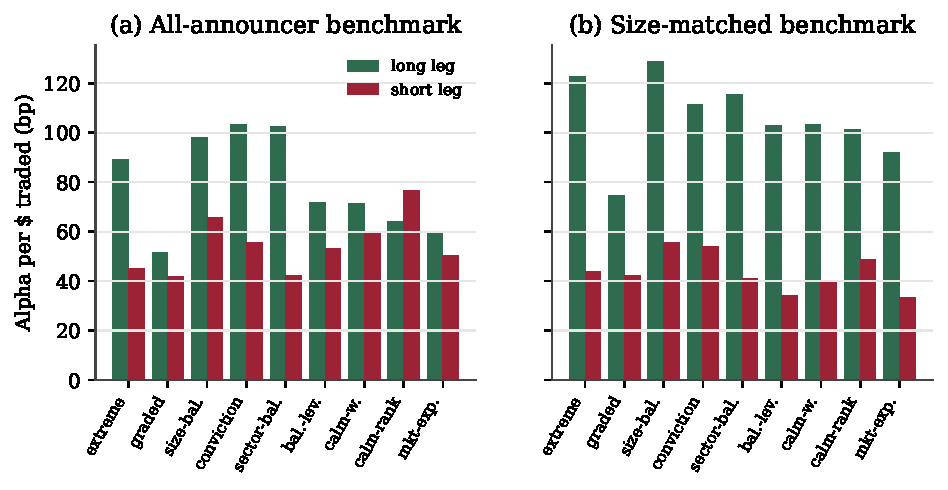
\includegraphics[width=\linewidth]{figures/fig_legs.pdf}
\caption{Alpha per dollar traded by leg under (a) the all-announcer benchmark and (b) the size-matched benchmark.}\label{fig:legs}
\end{figure}

\subsection{The best trade, and high-beta shorts}\label{sec:recipes}

We label every position with a \emph{recipe}: side (long or short) $\times$ how easily the stock trades (thin, mid, liquid) $\times$ beta (low, mid, high) $\times$ holding period
(at most 60 days, or longer), giving \stv{recipes.n} recipes per book.

\paragraph{The most profitable recipe.} In \stv{best.n_top} of the nine profiled books the single most profitable recipe is a long position in a thinly traded, low-beta stock held more than 60 days
(Table~\ref{tab:bestrecipe}). It uses \stv{best.money.min}--\stv{best.money.max} of the money, earns \stv{best.share.min}--\stv{best.share.max} of the alpha at \stv{best.bp.min}--\stv{best.bp.max} basis points per dollar, is
positive in \stv{best.qpos.min}--\stv{best.qpos.max} of quarters, and makes \stv{best.net.min} to \stv{best.net.max} of real profit per book. \stv{sent.best_eras}.

\begin{table}[t]\centering
\caption{The recipe ``long, thin, low-beta, held over 60 days'' in each book (size-matched alpha). ``Eras +'' is the number of the three eras in which its alpha is positive; ``Top recipe''
says whether it is the book's most profitable recipe. Source: \texttt{results/profiles\_recipes.csv}.}\label{tab:bestrecipe}
{\small
\begin{adjustbox}{max width=\linewidth}
\begin{tabular}{lrrrrrrrr}
\toprule
Book & Money & Alpha share & bp & $t$ & Quarters + & Eras + & Real \$ & Top recipe \\
\midrule
\sn{extreme_picks} & 2.2\% & 10.8\% & 490 & 4.8 & 71\% & 3/3 & \$2.8M & yes \\
\sn{graded_bets} & 2.2\% & 15.0\% & 522 & 6.5 & 76\% & 3/3 & \$3.2M & yes \\
\sn{size_balanced} & 2.4\% & 11.9\% & 529 & 4.9 & 68\% & 3/3 & \$3.0M & no \\
\sn{conviction_tilt} & 2.9\% & 17.0\% & 539 & 5.9 & 76\% & 3/3 & \$5.1M & yes \\
\sn{sector_balanced} & 3.1\% & 20.7\% & 648 & 6.6 & 78\% & 3/3 & \$3.9M & yes \\
\sn{balanced_leverage} & 2.1\% & 14.1\% & 530 & 5.8 & 76\% & 3/3 & \$5.8M & yes \\
\sn{calm_weighted} & 2.1\% & 13.0\% & 489 & 5.4 & 75\% & 2/3 & \$5.7M & yes \\
\sn{calm_rank_tilt} & 2.1\% & 10.1\% & 406 & 4.1 & 71\% & 2/3 & \$5.0M & yes \\
\sn{market_exposed} & 1.9\% & 13.1\% & 527 & 5.7 & 76\% & 2/3 & \$8.0M & yes \\
\bottomrule
\end{tabular}
\end{adjustbox}
}

\end{table}

\paragraph{High-beta shorts earn nothing, and cost real dollars.} Shorting a high-beta stock uses \stv{hbs.money.min}--\stv{hbs.money.max} of every book's money. \stv{sent.hbs}.
Their alpha lies between \stv{hbs.bp.min} and \stv{hbs.bp.max} basis points per dollar, and their real profit between \stv{hbs.real.min} and \stv{hbs.real.max}. Shorting low- and mid-beta stocks, by contrast, earns
\stv{lms.bp.min}--\stv{lms.bp.max} basis points per dollar ($t$ from \stv{lms.t.min} to \stv{lms.t.max}) in every book: same side, same signal, opposite verdicts, and beta is the dividing line. Even the good shorts lose real
dollars in \stv{lms.real.neg} of the nine books, because the average announcer beats the market; the long leg more than makes up for it. High-beta longs are unproven too (alpha \stv{hbl.bp.min}--\stv{hbl.bp.max} basis
points) but profitable in real dollars (\stv{hbl.real.min} to \stv{hbl.real.max}), so the problem is concentrated on the short side. Whether a rule such as ``no shorts in the highest-beta third'' would help is untested: removing those
positions also changes the hedge and the book's market exposure.

\begin{table}[t]\centering
\caption{High-beta shorts, low/mid-beta shorts and high-beta longs in each book: alpha per dollar (bp), quarter-clustered $t$, real profit and loss, and for high-beta shorts the number of eras with a real-dollar loss.
Source: \texttt{results/profiles\_beta\_legs.csv}.}\label{tab:betalegs}
{\small
\begin{adjustbox}{max width=\linewidth}
\begin{tabular}{lrrrrrrrrrr}
\toprule
 & \multicolumn{4}{c}{High-beta shorts} & \multicolumn{3}{c}{Low/mid-beta shorts} & \multicolumn{3}{c}{High-beta longs}\\
\cmidrule(lr){2-5}\cmidrule(lr){6-8}\cmidrule(lr){9-11}
Book & bp & $t$ & Real \$ & Losing eras & bp & $t$ & Real \$ & bp & $t$ & Real \$ \\
\midrule
\sn{extreme_picks} & $-$40 & $-$0.5 & $-$\$6.1M & 3/3 & 108 & 3.4 & $-$\$1.4M & 35 & 0.9 & \$4.3M \\
\sn{graded_bets} & 27 & 0.3 & $-$\$4.3M & 3/3 & 76 & 2.7 & $-$\$4.7M & 23 & 0.8 & \$4.7M \\
\sn{size_balanced} & $-$41 & $-$0.6 & $-$\$5.6M & 3/3 & 101 & 3.4 & $-$\$1.8M & 23 & 1.0 & \$3.7M \\
\sn{conviction_tilt} & 29 & 0.3 & $-$\$5.2M & 3/3 & 80 & 2.8 & $-$\$5.2M & 28 & 0.9 & \$6.0M \\
\sn{sector_balanced} & 1 & $-$0.0 & $-$\$3.6M & 3/3 & 81 & 2.6 & $-$\$3.3M & 73 & 0.7 & \$4.3M \\
\sn{balanced_leverage} & 6 & 0.1 & $-$\$8.3M & 3/3 & 73 & 2.6 & $-$\$7.1M & 52 & 0.5 & \$9.2M \\
\sn{calm_weighted} & 17 & 0.1 & $-$\$6.8M & 3/3 & 71 & 2.4 & $-$\$7.6M & 61 & 0.8 & \$8.7M \\
\sn{calm_rank_tilt} & 47 & 0.0 & $-$\$3.3M & 2/3 & 71 & 2.2 & $-$\$7.5M & 71 & 1.3 & \$6.6M \\
\sn{market_exposed} & 16 & 0.4 & $-$\$21.6M & 3/3 & 74 & 2.6 & $-$\$29.3M & 50 & 0.7 & \$23.0M \\
\bottomrule
\end{tabular}
\end{adjustbox}
}

\end{table}
\begin{figure}[t]\centering
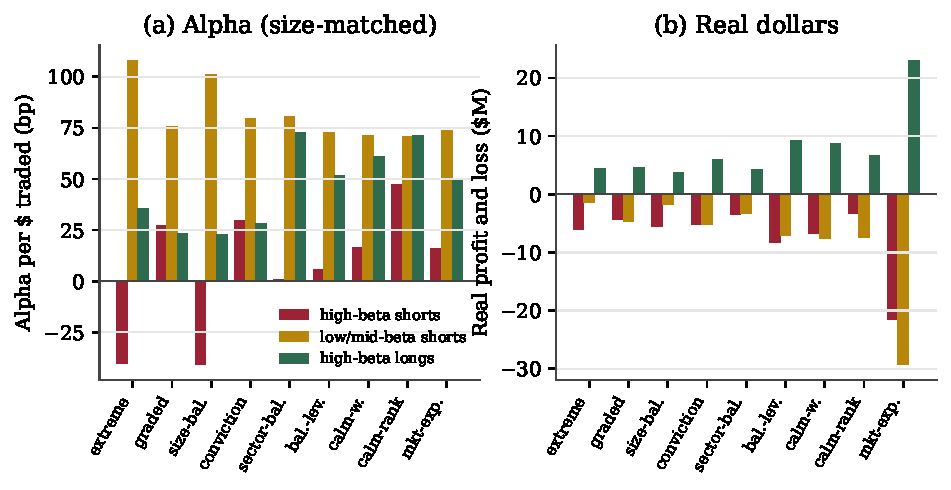
\includegraphics[width=\linewidth]{figures/fig_beta_legs.pdf}
\caption{(a) Alpha and (b) real dollars by beta group and side, for the nine profiled books.}\label{fig:betalegs}
\end{figure}

\paragraph{Most of the money sits in recipes that are not individually proven.} Between \stv{recipes.unproven.money.min} and \stv{recipes.unproven.money.max} of each book's money is in recipes with $|t|<2$, which still earn \stv{recipes.unproven.alpha.min} to \stv{recipes.unproven.alpha.max} of the alpha.
Moving along the lineage from \sn{extreme_picks} to \sn{calm_rank_tilt} changes the number of recipes that lose alpha from \stv{recipes.lose.first} (using \stv{recipes.lose.first.money} of the money) to \stv{recipes.lose.last} (\stv{recipes.lose.last.money}).
The winners and losers are drawn from the same pool: the best 1\% of positions earn \stv{tail.top.min}--\stv{tail.top.max} times a book's total alpha, and the worst 1\% lose \stv{tail.bot.min}--\stv{tail.bot.max} times it. Win rates are \stv{win.min}--\stv{win.max}, close to coin flips, so the profit is the small net
difference between large winners and large losers (Figure~\ref{fig:recipes}).

\begin{figure}[t]\centering
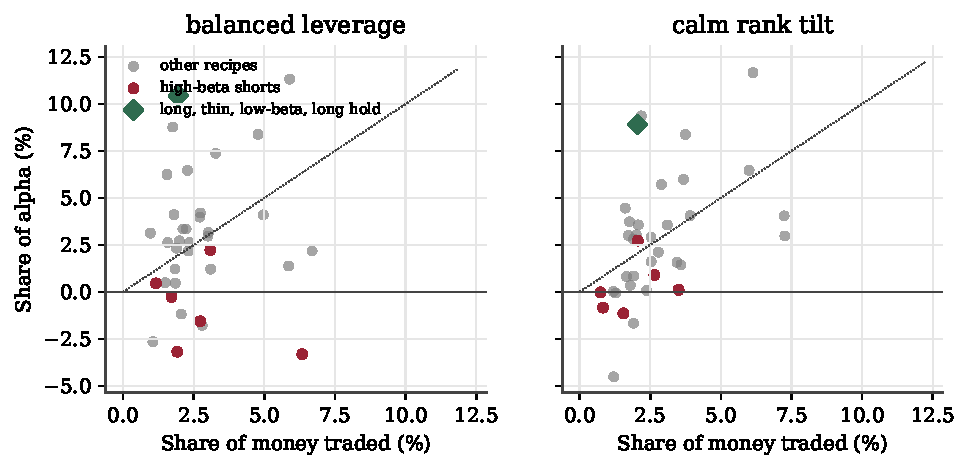
\includegraphics[width=\linewidth]{figures/fig_recipes.pdf}
\caption{Each point is one of the \stv{recipes.n} recipes: its share of the money traded against its share of alpha. Points above the dotted diagonal earn more than their share.
High-beta shorts (red) cluster at or below zero; the best recipe is the green diamond.}\label{fig:recipes}
\end{figure}

\subsection{Situations: what the money looks like when cut other ways}\label{sec:situations}

For the reference book \sn{balanced_leverage}, \texttt{results/situations\_all.csv} tests \stv{sit.n} situations (company size, how easily it trades, beta, hold length, period, and others), of which \stv{sit.n_engine} meet the ``engine'' standard
($t\ge2.5$, positive in at least two of three eras, and above the book's average). About \stv{sit.n} situations are tested per book, so a few look good by chance; the three-era rule is the guard against that. Table~\ref{tab:situations} shows the cuts
discussed here, and the paired-by-quarter contrasts are:
\begin{itemize}
  \item \textbf{Trading ease.} Thinnest-trading versus most-heavily-traded: \stv{sit.thin.a} versus \stv{sit.thin.b} basis points per dollar, a difference of \stv{sit.thin.diff} ($t=\stv{sit.thin.t}$). Smallest versus largest company: \stv{sit.small.a} versus \stv{sit.small.b}
        (difference \stv{sit.small.diff}, $t=\stv{sit.small.t}$). Company size and trading volume rank almost alike, so the data cannot separate them; in the joint regression neither survives once beta and hold length are held fixed (size \stv{drv.small.bp} basis points per standard deviation, $t=\stv{drv.small.t}$).
  \item \textbf{Hold length, with a caveat.} Holds over 90 days against holds up to 40 days: \stv{sit.hold.a} versus \stv{sit.hold.b} (difference \stv{sit.hold.diff}, $t=\stv{sit.hold.t}$). But each cell's hold length was estimated on the same history (Section~\ref{sec:decay}), so part of this is look-ahead.
  \item \textbf{Beta.} In the joint regression one standard deviation more beta costs \stv{drv.beta.bp} basis points per dollar ($t=\stv{drv.beta.t}$) with everything else fixed; longer hold windows add \stv{drv.hold.bp} ($t=\stv{drv.hold.t}$).
  \item \textbf{Era.} Alpha per dollar was \stv{eraA.bp} basis points in 1996--2001, \stv{eraB.bp} in 2002--07 and \stv{eraC.bp} in 2008--13, while the share of money traded in the last era rose to \stv{eraC.money}. Early versus late differ by \stv{sit.era.diff} ($t=\stv{sit.era.t}$).
  \item \textbf{Market direction.} Alpha per dollar is \stv{sit.mkt.a} when the market rose more than 5\% during the hold and \stv{sit.mkt.b} when it fell by more than 5\% (difference \stv{sit.mkt.diff}, $t=\stv{sit.mkt.t}$); a small and insignificant difference is what a market-neutral design should produce.
\end{itemize}

\begin{table}[t]\centering
\caption{Selected situations for \sn{balanced_leverage}, all-announcer benchmark. Money and alpha are shares of the book; $t$ is clustered by quarter; verdicts are defined in \texttt{docs/SITUATIONS.md}.}\label{tab:situations}
{\footnotesize
\begin{adjustbox}{max width=\linewidth}
\begin{tabular}{llrrrrl}
\toprule
Cut & Situation & Money & Alpha & bp/\$ & $t$ & Verdict \\
\midrule
Company size & size 1 (smallest) & 9\% & 4\% & 28 & 0.8 & UNPROVEN \\
Company size & size 2 & 19\% & 38\% & 125 & 3.9 & ENGINE \\
Company size & size 3 & 23\% & 27\% & 74 & 3.9 & ENGINE \\
Company size & size 4 & 24\% & 19\% & 49 & 3.5 & WORKS \\
Company size & size 5 (largest) & 24\% & 11\% & 29 & 2.4 & WORKS \\
\midrule
How easily traded & liquidity 1 (thinnest) & 7\% & 15\% & 133 & 3.6 & ENGINE \\
How easily traded & liquidity 2 & 20\% & 26\% & 81 & 3.1 & ENGINE \\
How easily traded & liquidity 3 & 24\% & 31\% & 80 & 3.9 & ENGINE \\
How easily traded & liquidity 4 & 24\% & 18\% & 47 & 2.6 & WORKS \\
How easily traded & liquidity 5 (most traded) & 24\% & 9\% & 24 & 1.7 & UNPROVEN \\
\midrule
Stock's market sensitivity & low--beta stocks & 32\% & 62\% & 121 & 5.7 & ENGINE \\
Stock's market sensitivity & mid--beta stocks & 34\% & 35\% & 64 & 3.5 & ENGINE \\
Stock's market sensitivity & high--beta stocks & 33\% & 3\% & 5 & $-$0.4 & UNPROVEN \\
\midrule
Hold length & <=40d & 34\% & 32\% & 59 & 3.0 & WORKS \\
Hold length & 41--60d & 25\% & 21\% & 51 & 2.7 & WORKS \\
Hold length & 61--90d & 33\% & 24\% & 45 & 2.1 & WORKS \\
Hold length & >90d & 8\% & 23\% & 185 & 3.0 & ENGINE \\
\midrule
Period & 1996--01 & 22\% & 43\% & 120 & 4.2 & ENGINE \\
Period & 2002--07 & 34\% & 44\% & 82 & 3.4 & ENGINE \\
Period & 2008--13 & 44\% & 13\% & 19 & 0.9 & UNPROVEN \\
\bottomrule
\end{tabular}
\end{adjustbox}
}

\end{table}

\begin{figure}[t]\centering
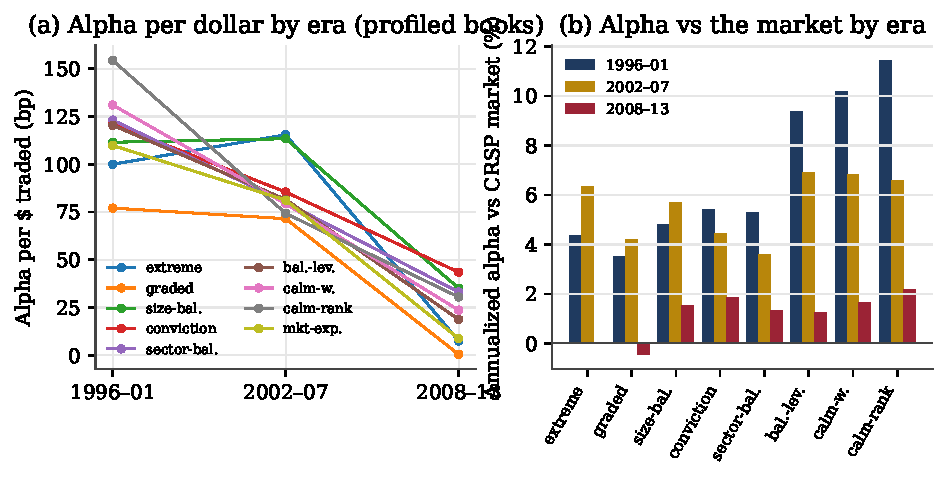
\includegraphics[width=\linewidth]{figures/fig_era.pdf}
\caption{Decay of alpha across eras. (a) Alpha per dollar traded for the nine profiled books. (b) Annualized alpha against the CRSP market for the eight market-neutral books.}\label{fig:era}
\end{figure}

Across the nine profiled books alpha per dollar was lower in 2008--13 than in 1996--2001 in \stv{era.all.fade.n} of nine, to between \stv{era.all.CA.min} and \stv{era.all.CA.max} of its 1996--2001 level. The mechanism section
predicts such decay if arbitrage capital has grown; the data are consistent with that and do not test it.

\subsection{Is the calm edge a volatility effect or a beta effect?}\label{sec:calm}

The volatility books rest on a finding about the signal (computed with the earlier within-quarter deciles, which this diagnostic was not rebuilt on): the D10$-$D1 spread is $+$\stv{vd.low} in the lowest tercile of stock-specific volatility, $+$\stv{vd.mid} in the middle and $+$\stv{vd.high} in the highest
($t$-statistics \stv{vd.low.t}, \stv{vd.mid.t}, \stv{vd.high.t}; difference between the extremes $t=\stv{vd.diff.t}$). Volatility alone does not change average returns, so it works as a \emph{sizing} input, not a filter; the
walk-forward filters \sn{volatility_filter} and \sn{calm_weighted_filter} (Sharpe \ssh{volatility_filter} and \ssh{calm_weighted_filter}) \stv{sent.filter_vs_sizing} sizing (\ssh{calm_weighted}).

Volatility and beta are correlated (correlation \stv{bv.corr} between a position's beta and its volatility percentile; \stv{bv.calm_lowbeta} of calm-tercile dollars are low-beta and \stv{bv.jumpy_highbeta} of jumpy-tercile dollars are
high-beta), so the calm edge could be a beta edge. We separate them with a $3\times3$ cut of the \sn{balanced_leverage} positions by beta tercile and idiosyncratic-volatility tercile (Table~\ref{tab:betavol}, Figure~\ref{fig:betavol}),
using the logic of \texttt{scripts/strategy\_profiles.py} on the saved positions. \stv{bv.stale_note}

\begin{table}[t]\centering
\caption{Alpha per dollar traded (bp, size-matched benchmark; quarter-clustered $t$ in parentheses) for \sn{balanced_leverage} positions cut by beta tercile and idiosyncratic-volatility
tercile. The right column and bottom row are the margins. Positions are read from \texttt{results/balanced\_leverage/positions.parquet}.}\label{tab:betavol}
{\small
\begin{adjustbox}{max width=\linewidth}
\begin{tabular}{lrrrr}
\toprule
 & Calm & Mid-vol & Jumpy & All volatilities \\
\midrule
Low-beta & 125 (6.9) & 123 (4.3) & 149 (2.8) & 128 (6.5) \\
Mid-beta & 43 (2.0) & 54 (2.5) & 96 (1.2) & 62 (3.6) \\
High-beta & 46 ($-$0.6) & 63 (1.0) & $-$23 ($-$0.8) & 13 ($-$0.1) \\
\midrule
All betas & 86 (6.4) & 77 (5.0) & 37 (1.4) &  \\
\bottomrule
\end{tabular}
\end{adjustbox}
}

\end{table}

Holding beta fixed, the calm-minus-jumpy gap averages \stv{bv.avg_calm_jumpy} basis points per dollar across the three beta terciles (within the low-beta tercile the jumpy positions earn
\stv{bv.size.cell.low_jumpy.bp} and the calm ones \stv{bv.size.cell.low_calm.bp}). Holding volatility fixed, the low-minus-high-beta gap averages \stv{bv.avg_low_high} basis points per dollar across the three volatility
terciles: \stv{bv.size.low_high.vol.calm.bp} for calm, \stv{bv.size.low_high.vol.mid.bp} for mid-volatility and \stv{bv.size.low_high.vol.jumpy.bp} for jumpy stocks. The larger margin is \stv{sent.bv.larger}. \stv{sent.bv.plain} The joint regression of Section~\ref{sec:situations}
gives (volatility \stv{drv.vol.bp} basis points per standard deviation with beta, size, liquidity and hold fixed, $t=\stv{drv.vol.t}$). The same cut under the all-announcer benchmark is written to \texttt{docs/paper/generated/tab\_betavol\_all.tex} for comparison.

\begin{figure}[t]\centering
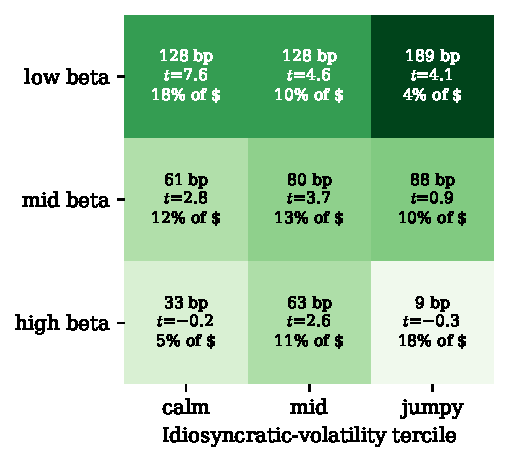
\includegraphics[width=0.62\linewidth]{figures/fig_beta_vol.pdf}
\caption{The $3\times3$ beta by volatility cut: alpha per dollar, quarter-clustered $t$-statistic and share of dollars in each cell.}\label{fig:betavol}
\end{figure}

\subsection{Selecting the sizing: what was tried}\label{sec:tried}

The volatility-sizing family was chosen from a search whose results are recorded in \texttt{docs/STRATEGIES.md} (\stv{trials.volrows} experiment rows, each with several parameter values: trim, tilt exponent, dropping deciles or holding cells,
a small-cap tilt, inverse-volatility powers, the rank-based tilt, and larger base units). The relevant fact for this paper is that the search was run on the full sample, so \sn{calm_weighted}'s construction and \sn{calm_rank_tilt}'s exponent are in-sample
choices, with the single split-sample check noted above. Section~\ref{sec:multiple} counts the trials that can be counted from files and deflates the Sharpe ratios accordingly.

%=====================================================================================
\section{The options strategy}\label{sec:options}
%=====================================================================================

The equity book earns the drift linearly. The options book earns it convexly. The question is how to choose, from the many contracts available on each event, the one that turns a modest directional edge into
compounding growth, and how to size it. We use the growth-optimal (Kelly) criterion \citep{Kelly1956,MacLeanThorpZiemba2011}, applied contract by contract.

\subsection{An empirical return law for each decile}

For announcement quarter $q$ and surprise decile $d$, the distribution of the underlying's 60-day return is estimated empirically from \emph{prior} quarters' events in the same decile (walk-forward, after a warm-up of \stv{kelly.warmup} quarters),
recentered on the trailing market drift so that the decile-specific tilt is not swamped by the unconditional equity premium. The pooled sample is cut at its quantiles into $M=\stv{kelly.states}$ equal-probability states.
State $s$ has conditional mean return $\rho_{ds}$ and probability $p_s=1/M$.

\subsection{Payoff and objective}

For an event with spot $S_0$, consider the call and put contracts $k$ of one expiry, with side $\phi_k\in\{+1,-1\}$, strike $K_k$, and premium $P_k$. The return on premium in state $s$ is
\begin{equation}
  R_{k,s}=\frac{\big(\phi_k\,[S_0(1+\rho_{ds})-K_k]\big)^+}{P_k}-1\ \in[-1,\infty).
  \label{eq:payoff}
\end{equation}
Staking a fraction $f$ of capital on contract $k$ yields expected log growth
\begin{equation}
  G_k(f)=\sum_{s=1}^{M}p_s\,\log\big(1+f\,R_{k,s}\big),\qquad
  g^\ast_k=\max_{f\in\F}G_k(f),\quad f^\ast_k=\arg\max_{f\in\F}G_k(f),
  \label{eq:growth}
\end{equation}
over a grid $\F=\{\stv{kelly.fmin},\dots,\stv{kelly.fmax}\}$ of \stv{kelly.nf} points. The event's contract is $k^\ast=\arg\max_k g^\ast_k$, and the event is traded only if $g^\ast_{k^\ast}>0$. The decile-conditioned
return law determines the direction on its own. In the funded book of \sn{options_cap20}, puts are \stv{ot.put.d1} of D1 selections and \stv{ot.put.d10} of D10 selections (Figure~\ref{fig:optsel}), and calls are \stv{ot.pct_calls}
of all funded trades: the selector found calls better value than puts even after bad news, which is what a return law centered on a positive trailing market drift produces.

\begin{proposition}[Well-posedness]\label{prop:wellposed}
For every $f\in\F$, $1+fR_{k,s}\ge 1-f>0$, so $G_k$ is finite and no bet can lose more than its stake. $G_k$ is strictly concave on $[0,1)$ unless every return is zero, with $G_k(0)=0$ and $G_k'(0)=\E[R_k]$.
In the continuum a positive stake is optimal if and only if the contract has positive expected return.
\end{proposition}

\begin{proposition}[Kelly ranking is Sharpe ranking to second order]\label{prop:sharpe}
Let $\mu_k=\E[R_k]$, $\sigma_k^2=\Var(R_k)$, and $m_k=\E[R_k^2]=\sigma_k^2+\mu_k^2$. Then
\begin{equation}
  G_k(f)\approx f\mu_k-\tfrac12 f^2 m_k,\qquad
  f^\ast_k\approx\frac{\mu_k}{m_k},\qquad
  g^\ast_k\approx\frac{\mu_k^2}{2m_k}=\frac12\cdot\frac{\mathrm{SR}_k^2}{1+\mathrm{SR}_k^2},
  \qquad \mathrm{SR}_k=\frac{\mu_k}{\sigma_k}.
\end{equation}
Among positive-edge contracts, ranking by $g^\ast$ equals ranking by the single-bet Sharpe ratio. A naive selector ranks by the expected return $\mu_k$, which is unbounded in the right tail and ignores risk.
\end{proposition}

\begin{proposition}[Minimum-stake hurdle]\label{prop:hurdle}
Since the smallest permitted stake is $f_{\min}>0$, a contract can be selected only if $G_k(f_{\min})>0$, which to second order reads
\begin{equation}
  \E[R_k]\;>\;\tfrac{f_{\min}}{2}\,\E[R_k^2].
  \label{eq:hurdle}
\end{equation}
\end{proposition}

The hurdle has economic content. A far-out-of-the-money strike that pays $80\times$ its premium with probability $4\%$ and otherwise expires worthless has $\E[R^2]\approx0.04\cdot80^2=256$. With $f_{\min}=\stv{kelly.fmin}$
it must clear $\E[R]>\tfrac12 f_{\min}\cdot256=6.4$, an expected return above 640\%. Near-the-money contracts with moderate second moments clear it with far smaller edges. The selector's objective is thus biased toward contracts
whose payoff is balanced across states, which is what a growth-optimal investor should prefer. Equation~\eqref{eq:growth} rewards a strike for the \emph{typical} payoff it delivers per unit of risk, not for the largest possible one.
Figure~\ref{fig:kelly} illustrates the mechanics on a stylized law; it is not estimated from data.

\begin{figure}[t]\centering
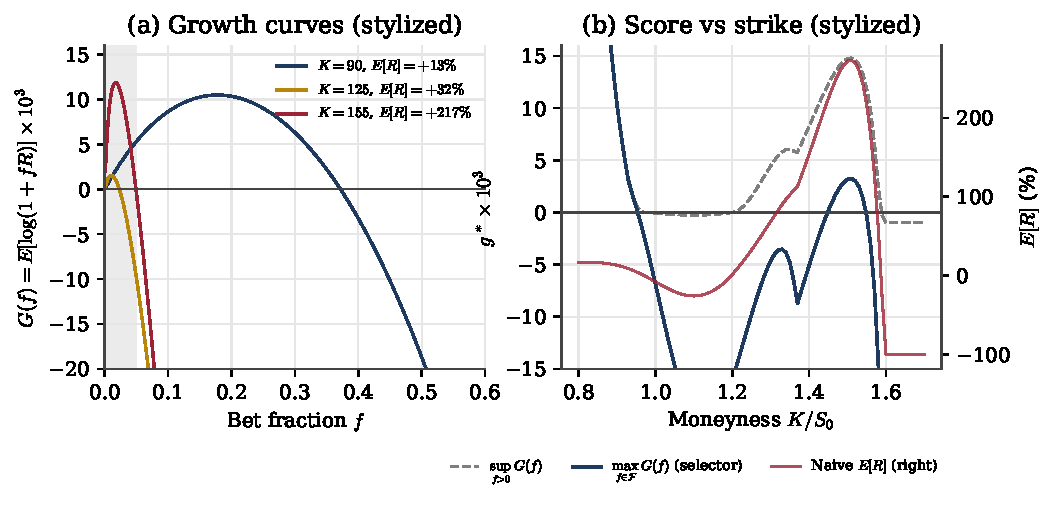
\includegraphics[width=\linewidth]{figures/fig_kelly_illustration.pdf}
\caption{\emph{Stylized illustration, not estimated from data}: a 40-state law with a diffuse body and a 4\% right-tail jump, calls priced at 30\% implied volatility with 120 days to expiry and valued at intrinsic at the horizon.
(a) Growth curves $G(f)$: the far-out-of-the-money strike ($K=155$) has the largest expected return and a growth peak inside the excluded region $f<f_{\min}$. (b) The continuous-stake supremum (dashed), the selector's grid score (solid)
and the naive expected return across strikes.}\label{fig:kelly}
\end{figure}

\subsection{From one bet to a portfolio: the premium budget}

A typical quarter offers over a thousand positive-edge events, and their single-bet fractions sum to many multiples of capital, so they cannot all be funded at $f^\ast$. The book instead fixes a budget: the premium outstanding across
all open positions may not exceed a fraction $c$ of trailing capital. Let $O_q$ be the premium still outstanding from earlier cohorts. The quarter's budget and each event's allocation are
\begin{equation}
  B_q=\big(c\,V_q-O_q\big)^+,\qquad
  \pi_i=B_q\,\frac{h_i}{\sum_{j\in\mathcal C_q}h_j},\qquad h_i=\stv{opt.halfkelly}\,f^\ast_{k^\ast(i)},
  \label{eq:alloc}
\end{equation}
so capital is allocated in proportion to each event's Kelly fraction (the factor \stv{opt.halfkelly} is the half-Kelly multiplier, which cancels in the proportion). Contracts are whole lots of \stv{opt.mult}; a round-trip cost of
\stv{opt.cost_pct} of premium, with a floor of \stv{opt.floor} per share (one option tick), is charged at entry. Positions are marked at the quoted prices on days \stv{opt.checkpoints} and exit at day \stv{opt.horizon}.

\begin{proposition}[Proportional allocation is fractional Kelly]\label{prop:fractional}
(a) The allocation is Kelly-proportional in relative terms, $\pi_i=\lambda_q f^\ast_i$ with $\lambda_q=B_q/\sum_jf^\ast_j$; its absolute scale is set only by the budget $c$.
(b) Under independence and the quadratic approximation of Proposition~\ref{prop:sharpe}, scaling the vector of single-bet Kelly stakes by $\lambda\in(0,1]$ gives portfolio growth $(2\lambda-\lambda^2)\sum_ig^\ast_i$ and a portfolio Sharpe ratio
\begin{equation}
  \mathrm{SR}_{\text{port}}=\frac{\sum_i\mu_i^2/m_i}{\big(\sum_i\mu_i^2\sigma_i^2/m_i^2\big)^{1/2}},
\end{equation}
which does not depend on $\lambda$ and grows as $\sqrt N$ in the number of bets.
(c) Every position's loss is bounded by its premium, so the loss on all open positions is at most $c$ times the capital at which they were sized.
\end{proposition}

Part (b) says that the book's Sharpe ratio comes from \emph{breadth}, not from leverage: \sn{options_cap20} funds about \stv{options_cap20.pos_per_year} small bets a year, an implied per-bet information coefficient of
\stv{options_cap20.implied_ic} (a lower bound on the true value, for the reason given for the equity book). It also predicts that return and volatility scale roughly linearly in the budget, with the Sharpe ratio nearly
unchanged, if the per-trade edge is real. In the corrected runs, raising the cap from 20\% to 30\% moves the return from \sret{options_cap20} to \sret{options_cap30}, the volatility from \svol{options_cap20} to \svol{options_cap30} and the Sharpe ratio from
\ssh{options_cap20} to \ssh{options_cap30}; before the fixes the same change moved them from \stv{options_cap20_prefix_fix.ret} to \stv{options_cap30_prefix_fix.ret} and the Sharpe ratio from \stv{options_cap20_prefix_fix.sharpe} to \stv{options_cap30_prefix_fix.sharpe}. The cap is a risk-appetite dial with a hard loss interpretation (part (c); the largest outstanding premium in the \sn{options_cap20} run was \stv{options_cap20.maxprem} of NAV), not a source of
extra edge. The caps 20\% and 30\% are in-sample choices: they were fixed after the earlier results and not re-chosen after the corrections, and larger caps (40\%) exist only in the legacy runs.

\subsection{Results after bid/ask fills}\label{sec:optresults}

\begin{table}[t]\centering
\caption{Kelly options books under each fill convention. The top block is the current convention (ask in, bid out at the final checkpoint, dead options marked at half the ask, or zero in the pessimistic bound);
the middle block is the mid-price convention with a tick floor, with and without the point-in-time deciles; the bottom block is the originally reported convention. Source: \texttt{results/<name>/summary.json}.}\label{tab:options}
{\small
\begin{adjustbox}{max width=\linewidth}
\begin{tabular}{llrrrrrl}
\toprule
Book & Dead-quote mark & Return & Vol & Sharpe & Max DD & Calmar & Role \\
\midrule
\sn{options_cap20} & zero\_bid\_half\_ask & 4.12\% & 2.30\% & 1.77 & $-$13.8\% & 0.30 & validated headline \\
\sn{options_cap30} & zero\_bid\_half\_ask & 5.69\% & 3.61\% & 1.55 & $-$22.3\% & 0.26 & validated \\
\sn{options_worst_case} & zero\_bid\_zero & 2.34\% & 2.37\% & 0.99 & $-$17.1\% & 0.14 & pessimistic bound \\
\midrule
\sn{options_cap20_legacy} & carry\_last & 8.58\% & 2.18\% & 3.78 & $-$10.3\% & 0.83 & overstated \\
\sn{options_cap30_legacy} & carry\_last & 12.26\% & 3.33\% & 3.49 & $-$17.4\% & 0.70 & overstated \\
\sn{options_cap40_legacy} & carry\_last & 15.79\% & 4.50\% & 3.28 & $-$23.9\% & 0.66 & overstated \\
\bottomrule
\end{tabular}
\end{adjustbox}
}

\end{table}

Table~\ref{tab:options} reports the books. With the current convention \sn{options_cap20} earns \sret{options_cap20} a year at \svol{options_cap20} volatility, a Sharpe ratio of \ssh{options_cap20} and a maximum
drawdown of \sdd{options_cap20}. It \stv{sent.opt_edge}. The 30\% book \sn{options_cap30} earns \sret{options_cap30} (a \stv{sent.opt_cap30_sign} return) at a Sharpe ratio of \ssh{options_cap30}, and the pessimistic bound
\sn{options_worst_case} earns \sret{options_worst_case}. These books were labelled ``validated'' because their construction was fixed before the result; that label does not imply an edge. The funded \sn{options_cap20} book
has \stv{ot.n} trades. Net profit over the sample is \stv{ot.net_M} on \stv{ot.prem_M} of premium paid (\stv{ot.net_over_prem}); the win rate is \stv{ot.win} and the median trade returns
\stv{ot.median} of premium. \stv{ot.pct_calls} of funded trades are calls, producing \stv{ot.pct_pnl_calls} of gross profit, and puts are \stv{ot.put.d1} of D1 selections against \stv{ot.put.d10} of D10 selections
(Figure~\ref{fig:optsel}). Net profit is small relative to premium at risk, so shares of it (by year, or by the best trades) are unstable and we do not report them; entry years \stv{ot.loss_years} lose.

\begin{figure}[t]\centering
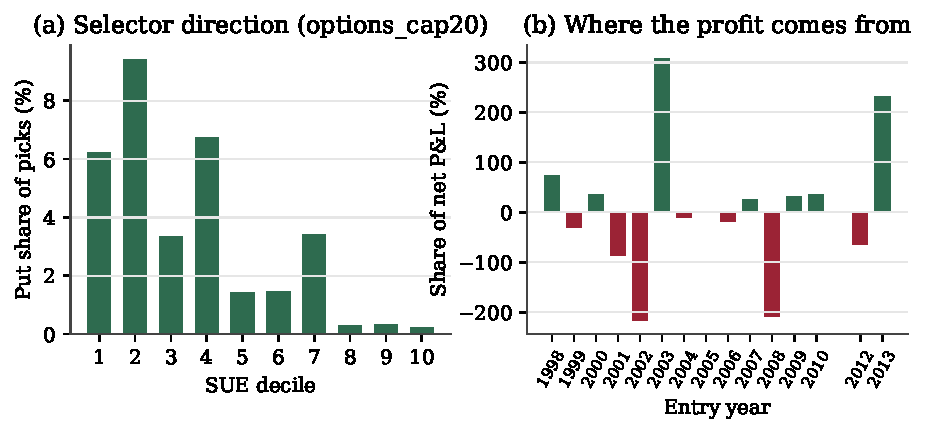
\includegraphics[width=\linewidth]{figures/fig_options_trades.pdf}
\caption{Funded \sn{options_cap20} trades. (a) Share of puts among the selector's picks by SUE decile. (b) Share of net profit by entry year (the denominator is small, so the shares are noisy).}\label{fig:optsel}
\end{figure}

\subsection{Why the earlier numbers were higher}\label{sec:quoteerror}

The options result has been revised three times, and each revision lowered it. The original backtest valued each position at days \stv{opt.checkpoints} from the contract's mid quote and, when a quote was missing, \emph{carried the previous quote forward}.
\stv{opt.missing60} of picks had no mid quote at 60 days, and re-querying OptionMetrics showed that \stv{opt.zerobid} of those were not missing: the bid was zero, so the option had died and nobody would buy it. Carrying its last live price forward never marks a dying
option down, which flatters exactly the contracts that die. Marking a dead quote at half the ask moved the 20\% book from \stv{optchain.legacy.ret} (Sharpe \stv{optchain.legacy.sh}) to \stv{optchain.mark.ret} (\stv{optchain.mark.sh}), and a floor of one option tick of round-trip cost
per share moved it to \stv{optchain.floor.ret} (\stv{optchain.floor.sh}); this is the number earlier drafts of this paper reported as corrected (and \stv{optchain.zero.ret}, Sharpe \stv{optchain.zero.sh}, if dead options are worth zero).

The last correction is the fill itself. The book had been charged a flat percentage of the mid price; it actually pays the ask when it buys and receives the bid when it sells. On the same contracts and the same deciles, bid/ask fills alone move the 20\% book
from \stv{ladder.options_cap20.published.ret} / \stv{ladder.options_cap20.published.sharpe} to \stv{ladder.options_cap20.fix3_only_bidask.ret} / \stv{ladder.options_cap20.fix3_only_bidask.sharpe}, and the 30\% book from
\stv{ladder.options_cap30.published.ret} / \stv{ladder.options_cap30.published.sharpe} to \stv{ladder.options_cap30.fix3_only_bidask.ret} / \stv{ladder.options_cap30.fix3_only_bidask.sharpe} (Table~\ref{tab:ladderop}). The point-in-time deciles alone,
with mid fills, change the 20\% book from \stv{ladder.options_cap20.published.ret} to \stv{ladder.options_cap20.fix2_only_midfill.ret}, a difference small enough to be noise. The earlier drafts' options headline
(\sret{options_cap30_legacy} and a Sharpe ratio of \ssh{options_cap30_legacy}, the 30\% book under the original convention) was therefore an artifact of the fill convention, and the 20\% book under the original convention reported \stv{optchain.legacy.ret} against \sret{options_cap20} now. Figure~\ref{fig:optaudit} shows the same book under four conventions.

\begin{table}[t]\centering
\caption{Options books with each fix applied in turn (return / Sharpe ratio). Source: the attribution ladder in \texttt{docs/paper/cache/ladders/options\_ladder.csv}, produced by the fixes work.}\label{tab:ladderop}
{\small
\begin{adjustbox}{max width=\linewidth}
\begin{tabular}{lrrrr}
\toprule
Book & Published & Bid/ask fills only & Point-in-time deciles only (mid fills) & All fixes \\
\midrule
\sn{options_cap20} & 4.12\% / 1.77 & 0.16\% / 0.09 & 4.43\% / 1.85 & 0.28\% / 0.16 \\
\sn{options_cap30} & 5.69\% / 1.55 & $-$0.27\% / $-$0.08 & 6.10\% / 1.62 & $-$0.10\% / $-$0.02 \\
\sn{options_worst_case} & 2.34\% / 0.99 & $-$1.11\% / $-$0.57 & -- & $-$1.04\% / $-$0.52 \\
\sn{options_cap20_legacy} & 8.58\% / 3.78 & -- & -- & -- \\
\bottomrule
\end{tabular}
\end{adjustbox}
}

\end{table}

\begin{figure}[t]\centering
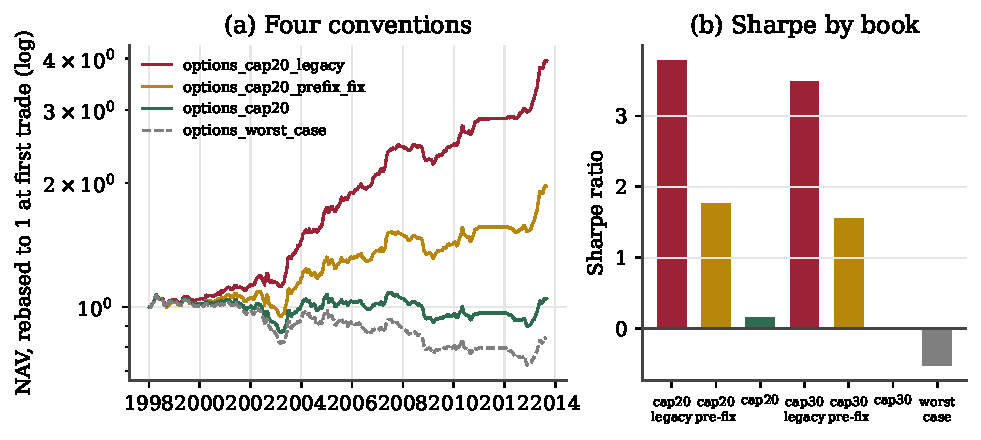
\includegraphics[width=\linewidth]{figures/fig_options_audit.pdf}
\caption{(a) NAV of the 20\% book under the original convention, the mid-fill convention with a tick floor (reported before the fixes), the current bid/ask convention and the pessimistic bound. (b) Sharpe ratios by book and convention.}\label{fig:optaudit}
\end{figure}

\paragraph{Remaining weaknesses.} The Kelly selector still scores contracts at the mid while the book pays the ask, so selection and execution use different prices (re-scoring at the ask is a documented follow-up, not done). There is no market impact,
although the book opens about \stv{options_cap20.pos_per_year} trades a year. The first walk-forward distributions rest on \stv{kelly.warmup} quarters. The caps (20\% and 30\%) and the half-Kelly multiplier were fixed before the result and were not re-chosen after
the corrections. With a near-zero edge these dials mainly scale risk.


%=====================================================================================
\section{The combined strategy}\label{sec:combined}
%=====================================================================================

\subsection{The diversification argument and what survives of it}

Let the two sleeves have annualized volatilities $\sigma_e,\sigma_o$, correlation $\rho$, and sleeve weights $w_e,w_o$ (multiples of each sleeve's own sizing, which need not sum to one). The blend's volatility is
\begin{equation}
  \sigma_p^2=w_e^2\sigma_e^2+w_o^2\sigma_o^2+2w_ew_o\rho\,\sigma_e\sigma_o.
  \label{eq:blendvar}
\end{equation}
Over the options book's active window the daily correlation between \sn{calm_weighted} and \sn{options_cap20} is \stv{corr.eo} (monthly: \stv{corr.eo.monthly} over \stv{corr.eo.months} months); the equity sleeve's correlation with the market is \stv{corr.em} and the options
sleeve's is \stv{corr.om}. A low correlation lowers the blend's risk, which is useful only if the sleeve that is added earns a return for the risk it carries. Earlier drafts argued that it did: the options sleeve then earned
\stv{options_cap20_prefix_fix.ret} a year at a Sharpe ratio of \stv{options_cap20_prefix_fix.sharpe}. With bid/ask fills it earns \sret{options_cap20} at \ssh{options_cap20}, so the argument now rests on a sleeve with no measurable edge. The economic reason for the low
correlation is unchanged (the equity book's short leg loses in a rally led by low-quality, heavily shorted stocks, the regime that produces momentum crashes \citep{DanielMoskowitz2016}, while a purchased option loses at most its premium), but it is a
reason for \emph{hedging}, not evidence of a premium.

\subsection{The blends}

The blends are $\sn{hedged_blend}=\stv{hedged_blend.w_calm_weighted}\times\sn{calm_weighted}+\stv{hedged_blend.w_options_cap20}\times\sn{options_cap20}$ on one NAV rebalanced daily, and
$\sn{calm_blend}=\stv{calm_blend.w_calm_rank_tilt}\times\sn{calm_rank_tilt}+\stv{calm_blend.w_options_cap20}\times\sn{options_cap20}$ (inheriting the in-sample status of its equity sleeve). The multiples were chosen to give each sleeve about equal stand-alone
volatility when the options sleeve looked far stronger, and they were not re-optimised after the corrections. \sn{legacy_blend} uses the options sleeve under the original convention and is an overstated upper bound, not a result.

\begin{table}[t]\centering
\caption{The two sleeves and the blends, with Sharpe ratios by era. The blocks marked ``before the fixes'' are the saved pre-correction runs. Source: \texttt{results/<name>/summary.json}.}\label{tab:blend}
{\small
\begin{adjustbox}{max width=\linewidth}
\begin{tabular}{llrrrrrrr}
\toprule
Book & Role & Return & Vol & Sharpe & Max DD & Sh 96--01 & Sh 02--07 & Sh 08--13 \\
\midrule
\sn{calm_weighted} & equity sleeve & 5.64\% & 4.51\% & 1.24 & $-$17.5\% & 2.03 & 1.54 & 0.29 \\
\sn{options_cap20} & options sleeve & 0.28\% & 1.92\% & 0.16 & $-$18.9\% & 0.07 & 0.31 & 0.00 \\
\midrule
\sn{hedged_blend} & validated & 4.90\% & 4.46\% & 1.09 & $-$21.8\% & 1.82 & 1.31 & 0.25 \\
\sn{calm_blend} & research & 5.80\% & 4.48\% & 1.28 & $-$20.1\% & 2.13 & 1.36 & 0.43 \\
\midrule
\sn{hedged_blend_prefix_fix} & before the fixes & 11.33\% & 4.83\% & 2.25 & $-$16.7\% & 2.41 & 2.70 & 1.91 \\
\sn{calm_blend_prefix_fix} & before the fixes & 12.43\% & 4.73\% & 2.50 & $-$15.5\% & 2.92 & 2.84 & 2.10 \\
\sn{legacy_blend} & overstated legacy & 14.25\% & 4.18\% & 3.21 & $-$9.9\% & 2.79 & 4.64 & 2.61 \\
\bottomrule
\end{tabular}
\end{adjustbox}
}

\end{table}

\paragraph{Results.} \sn{hedged_blend} has \stv{sent.blend_vs_equity}. Its Sharpe ratio \stv{sent.blend_vs_sleeves}, and it is above the weaker sleeve's \stv{sent.blend_sleeve_in_eras}. Before the corrections it earned \stv{hedged_blend_prefix_fix.ret} with a Sharpe ratio of
\stv{hedged_blend_prefix_fix.sharpe}. The sleeves' Sharpe ratios by era are \stv{calm_weighted.shA}, \stv{calm_weighted.shB}, \stv{calm_weighted.shC} (equity) and \stv{options_cap20.shA}, \stv{options_cap20.shB}, \stv{options_cap20.shC} (options): \stv{sent.sleeve_lead}.
The blend's beta against the market is \stv{hedged_blend.beta_mkt}. \sn{calm_blend} earns \sret{calm_blend} at \svol{calm_blend} volatility (Sharpe \ssh{calm_blend}, drawdown \sdd{calm_blend}); before the corrections \stv{calm_blend_prefix_fix.ret} and \stv{calm_blend_prefix_fix.sharpe}.
Comparing each blend with its equity sleeve (Table~\ref{tab:blend}) is the right test of whether the options sleeve adds anything; we do not claim that it does.

\begin{figure}[t]\centering
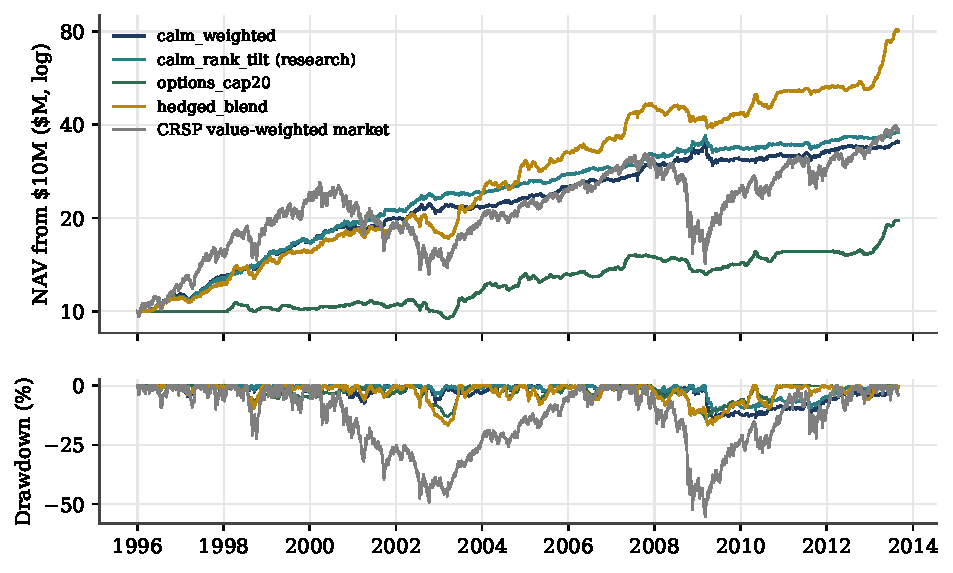
\includegraphics[width=\linewidth]{figures/fig_nav_drawdown.pdf}
\caption{NAV (log scale, \$10M start) and drawdowns of the validated equity book, the research equity book, the options book, the validated blend and the CRSP value-weighted market, 1996 to August 2013.}\label{fig:nav}
\end{figure}

\subsection{Calendar years}

\begin{table}[t]\centering
\caption{Calendar-year returns (\%) of \sn{calm_weighted}, \sn{options_cap20} and the market. The options book has no trades before 1998 and no data for 2011 (the source file is corrupt), and its 2013 figure covers
January to August; dashes mark years without trades.}\label{tab:calendar}
{\small
\begin{adjustbox}{max width=\linewidth}
\begin{tabular}{lrrr@{\hspace{2em}}lrrr}
\toprule
Year & Equity & Options & Market & Year & Equity & Options & Market \\
\midrule
1996 & 14.0\% & -- & 21.2\% & 2005 & 8.5\% & $-$0.5\% & 7.3\% \\
1997 & 14.4\% & -- & 30.4\% & 2006 & 4.9\% & 4.2\% & 16.2\% \\
1998 & 14.8\% & 2.9\% & 22.3\% & 2007 & 12.9\% & 9.3\% & 7.3\% \\
1999 & 12.0\% & $-$1.2\% & 25.7\% & 2008 & 10.6\% & $-$10.0\% & $-$38.2\% \\
2000 & 11.3\% & 4.0\% & $-$11.3\% & 2009 & $-$6.9\% & 6.1\% & 31.2\% \\
2001 & 6.8\% & $-$0.3\% & $-$11.0\% & 2010 & 2.6\% & 9.2\% & 17.7\% \\
2002 & 5.7\% & $-$6.1\% & $-$20.9\% & 2011 & 4.0\% & -- & $-$1.1\% \\
2003 & 2.5\% & 18.8\% & 33.1\% & 2012 & 1.8\% & $-$1.7\% & 15.8\% \\
2004 & 7.6\% & 12.3\% & 13.0\% & 2013 & 5.5\% & 27.8\% & 30.5\% \\
\bottomrule
\end{tabular}
\end{adjustbox}
}

\end{table}

The equity book has \stv{cal.n_eq_loss_years} losing calendar year(s) in 1996--2013 (\stv{cal.eq.loss_years}); the worst was \stv{cal.eq.worst} in \stv{cal.eq.worst.year}, when the options book returned \stv{cal.op.in.eqworst}; in 2008 the equity book returned \stv{cal.eq.2008} and the options book
\stv{cal.op.2008} (Table~\ref{tab:calendar}, Figure~\ref{fig:cal}). Two years are thin evidence either way.

\begin{figure}[t]\centering
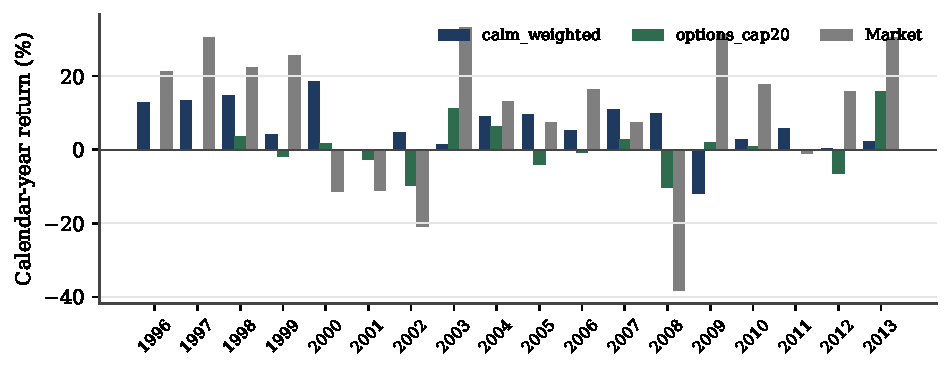
\includegraphics[width=\linewidth]{figures/fig_calendar_returns.pdf}
\caption{Calendar-year returns of the equity book, the options book and the CRSP value-weighted market.}\label{fig:cal}
\end{figure}


%=====================================================================================
\section{Capacity and the risk-budget dial}\label{sec:capacity}
%=====================================================================================

\begin{proposition}[Concave capacity frontier]\label{prop:capacity}
Let $b$ scale the book, and assume expected abnormal return per dollar, $\alpha_i$, is non-increasing in a stock's liquidity. Then the marginal expected alpha per dollar of additional capital is non-increasing in $b$.
Holding the volatility cost fixed, expected arithmetic return is concave in $b$, and the geometric return (arithmetic return less $\tfrac12\sigma^2(b)$) has an interior maximum.
\end{proposition}

Economically, as capital grows, the stocks with the highest drift saturate their liquidity limits first. Additional capital flows to larger, lower-drift names, while risk rises in proportion to gross exposure. The return of
the \sn{balanced_leverage} construction at a six-times cap, swept over the base unit $b$ (Table~\ref{tab:frontier}, Figure~\ref{fig:frontiers}a; a pre-correction sweep file), \stv{sent.sweep_peak}; the maximum is at $b=\stv{sweep.peak.b}\times10^{-3}$ with a return of
\stv{sweep.peak.ret}, where \stv{sweep.peak.cap} of positions are volume-capped, and falls to \stv{sweep.last.ret} at $b=\stv{sweep.last.b}\times10^{-3}$ with \stv{sweep.last.cap} capped. The rule used to choose $b$ for the \sn{*_max}
books (highest return subject to a Sharpe ratio of at least \stv{rule.sharpe} and a drawdown no worse than $-$\stv{rule.dd}) selects $b=\stv{sweep.rule.b}\times10^{-3}$ from this grid, in sample. \stv{sent.sweepnote}

\begin{table}[t]\centering
\caption{Equity capacity frontier: sweep over the base-unit fraction $b$ at a six-times gross cap (all other parameters fixed); the row used for \sn{balanced_leverage_max} is in bold. This is the pre-correction sweep, shown for the shape of the frontier only; the saved corrected run at the chosen unit earns \sret{balanced_leverage_max}. Source:
\texttt{data/sweep\_aggressive\_strategy6.csv}.}\label{tab:frontier}
{\small
\begin{adjustbox}{max width=\linewidth}
\begin{tabular}{rrrrrrr}
\toprule
$b\ (\times10^{-3})$ & Return & Vol & Sharpe & Max DD & ADV-capped & Avg gross / initial cap. \\
\midrule
4.5 & 7.26\% & 6.71\% & 1.08 & $-$25.1\% & 15.8\% & 6.4$\times$ \\
6 & 8.23\% & 8.28\% & 1.00 & $-$30.3\% & 21.1\% & 9.5$\times$ \\
7.5 & 8.93\% & 9.68\% & 0.93 & $-$34.7\% & 25.9\% & 12.6$\times$ \\
9 & 9.30\% & 10.92\% & 0.87 & $-$37.3\% & 31.9\% & 15.5$\times$ \\
10.5 & 9.07\% & 12.00\% & 0.78 & $-$40.8\% & 39.4\% & 16.7$\times$ \\
\textbf{12} & \textbf{8.35\%} & \textbf{12.82\%} & \textbf{0.69} & \textbf{$-$44.9\%} & \textbf{48.6\%} & \textbf{16.5$\times$} \\
15 & 7.92\% & 13.69\% & 0.63 & $-$44.8\% & 62.9\% & 15.7$\times$ \\
18 & 7.95\% & 14.63\% & 0.60 & $-$43.0\% & 71.3\% & 15.3$\times$ \\
21 & 6.89\% & 15.77\% & 0.50 & $-$43.0\% & 77.1\% & 12.9$\times$ \\
24 & 5.81\% & 16.98\% & 0.42 & $-$46.8\% & 80.8\% & 11.2$\times$ \\
30 & 3.83\% & 19.04\% & 0.29 & $-$52.8\% & 85.3\% & 9.9$\times$ \\
36 & 2.82\% & 21.49\% & 0.24 & $-$54.3\% & 88.2\% & 7.9$\times$ \\
\bottomrule
\end{tabular}
\end{adjustbox}
}

\end{table}

\begin{figure}[t]\centering
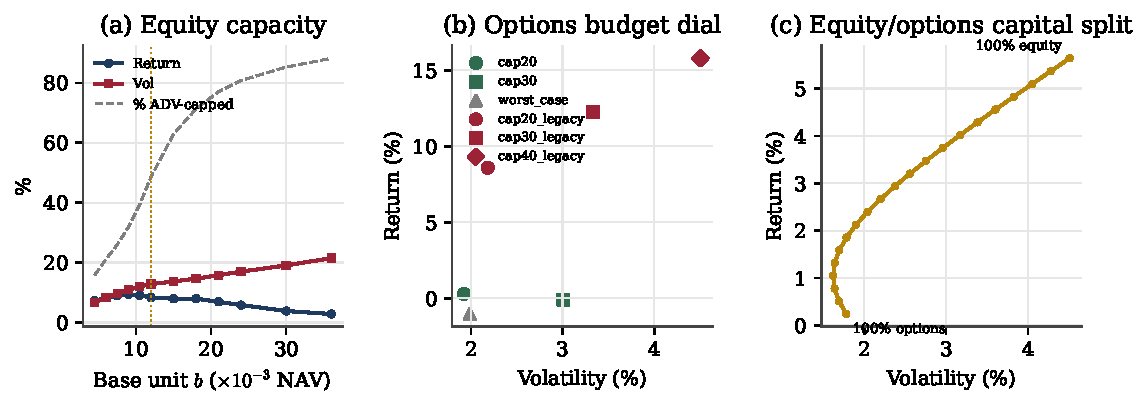
\includegraphics[width=\linewidth]{figures/fig_frontiers.pdf}
\caption{(a) Equity: return, volatility and share of volume-capped positions against the base unit. The dotted line marks the chosen unit. (b) Options: return and volatility of the premium-cap books
(green: current bid/ask fills; red: original convention). (c) Capital-split frontier of the equity and options sleeves from \texttt{results/portfolio/frontier.csv} (\stv{frontier.equity} with \sn{options_cap20}).}\label{fig:frontiers}
\end{figure}

Equity return is capacity-bound. For options, the premium cap $c$ is a risk-appetite dial that scales risk; with the corrected fills it scales a near-zero return (Figure~\ref{fig:frontiers}b). The practical limits on the options book lie outside the backtest: quoted width, depth and market impact in single-name options.
Among capital-split blends (sleeve weights summing to one; panel c), the Sharpe ratio runs from \stv{frontier.sh.min} to \stv{frontier.sh.max} and peaks at \stv{frontier.best.w} equity (return \stv{frontier.best.ret}, volatility \stv{frontier.best.vol}), to be compared with \sn{hedged_blend}, which uses sleeve multiples above one (return \sret{hedged_blend}, volatility \svol{hedged_blend}).

%=====================================================================================
\section{Statistical robustness and backtest hygiene}\label{sec:audit}
%=====================================================================================

\subsection{Multiple testing}\label{sec:multiple}

Both books were selected from a family of trials, so we deflate their Sharpe ratios \citep{BaileyLopezdePrado2014}. For $N$ trials whose annualized Sharpe ratios have variance $V$, the expected maximum under the null is
\begin{equation}
  \widehat{\mathrm{SR}}_0=\sqrt{V}\Big[(1-\gamma_E)\,\Phi^{-1}\!\big(1-\tfrac1N\big)+\gamma_E\,\Phi^{-1}\!\big(1-\tfrac{1}{Ne}\big)\Big],
\end{equation}
where $\gamma_E$ is the Euler--Mascheroni constant. The deflated Sharpe ratio is the probabilistic Sharpe ratio \citep{BaileyLopezdePrado2012} measured against $\widehat{\mathrm{SR}}_0$, allowing for the skewness $\hat\gamma_3$ and
kurtosis $\hat\gamma_4$ of the returns:
\begin{equation}
  \mathrm{DSR}=\Phi\!\left(\frac{(\widehat{\mathrm{SR}}-\widehat{\mathrm{SR}}_0)\sqrt{T-1}}{\sqrt{1-\hat\gamma_3\widehat{\mathrm{SR}}+\tfrac{\hat\gamma_4-1}{4}\widehat{\mathrm{SR}}^2}}\right),
\end{equation}
with Sharpe ratios in per-period units and $T$ the number of active days.

\paragraph{How the trials were counted.} Every count is a count of entries in a committed file. For equity, $N=\stv{trials.eq}$: the \stv{trials.eq.runs} equity runs in \texttt{results/} (the \stv{n_registered_equity} registered strategies, with their pre-correction \texttt{*\_legacy} twins, which were trials too) plus the
\stv{trials.eq.sweeprows} rows in the \stv{trials.eq.sweepfiles} sweep files \texttt{data/sweep\_*.csv} (base unit, liquidity cap, leverage and trim sweeps for the numbered designs). The standard deviation of their Sharpe ratios is
\stv{trials.eq.sd}. For options, $N=\stv{trials.op}$: the \stv{trials.op.runs} options runs in \texttt{results/} plus the \stv{trials.op.oldrows} rows of the \stv{trials.op.oldfiles} horizon-by-budget comparison files from before the correction (four constructions $\times$ six
holding horizons); the standard deviation of their Sharpe ratios is \stv{trials.op.sd}, but across only the \stv{trials.op.n_corr} runs not under the original convention it is \stv{trials.op.sd_corr}. These counts are lower bounds. The experiment tables recorded in \texttt{docs/STRATEGIES.md}
(\stv{trials.volrows} rows of several parameter values each) are not files with Sharpe ratios and are not counted, nor are discarded designs that left no file. Table~\ref{tab:dsrsens} therefore shows how the answer moves with $N$.

\begin{table}[t]\centering
\caption{Probabilistic and deflated Sharpe ratios on active-period daily returns. $N$ is the counted number of trials; $\widehat{\mathrm{SR}}_0$ is the expected maximum Sharpe ratio under the null for that $N$ and the dispersion of the counted trials;
$N^\ast$ is the number of trials at which the DSR would fall below 0.95 (same dispersion).}\label{tab:dsr}
{\small
\begin{adjustbox}{max width=\linewidth}
\begin{tabular}{lrrrrrr}
\toprule
Book & $N$ & Active Sharpe & $\widehat{\mathrm{SR}}_0$ & PSR vs 0 & DSR & $N^\ast$ for DSR$<0.95$ \\
\midrule
\sn{calm_weighted} & 387 & 1.28 & 0.81 & 1.000 & 0.97 & 1{,}000 \\
\sn{calm_rank_tilt} & 387 & 1.52 & 0.81 & 1.000 & 1.00 & 32{,}680 \\
\sn{balanced_leverage} & 387 & 1.13 & 0.81 & 1.000 & 0.91 & 164 \\
\sn{balanced_leverage_max} & 387 & 0.71 & 0.81 & 0.999 & 0.34 & 6 \\
\sn{options_cap20} & 35 & 0.17 & 2.82 & 0.739 & 0.00 & 2 \\
\sn{options_cap30} & 35 & $-$0.02 & 2.82 & 0.473 & 0.00 & 2 \\
\sn{hedged_blend} & 387 & 1.13 & 0.81 & 1.000 & 0.91 & 181 \\
\sn{calm_blend} & 387 & 1.33 & 0.81 & 1.000 & 0.99 & 2{,}131 \\
\bottomrule
\end{tabular}
\end{adjustbox}
}

\end{table}

\paragraph{Results.} The validated equity book \sn{calm_weighted} \stv{sent.eq_dsr} (DSR \stv{calm_weighted.dsr}); its break-even is about \stv{calm_weighted.dsr_Nstar} independent trials, against the \stv{trials.eq} counted.
The research book \sn{calm_rank_tilt} \stv{sent.crt_dsr} the bar at the counted $N$ (DSR \stv{calm_rank_tilt.dsr}). The six-times-leveraged \sn{balanced_leverage_max} has a DSR of \stv{balanced_leverage_max.dsr} and a break-even of
\stv{balanced_leverage_max.dsr_Nstar} trials. The options book \sn{options_cap20} \stv{sent.opt_dsr}: its DSR is \stv{options_cap20.dsr} with the dispersion of all counted trials and \stv{options_cap20.dsr_corr} with the dispersion of the runs not under the original convention only
(\stv{options_cap30.dsr} and \stv{options_cap30.dsr_corr} for \sn{options_cap30}); with a probabilistic Sharpe ratio against zero of only \stv{options_cap20.psr}, the options book does not clear a zero benchmark either, so the deflation is moot.
The deflation does not cover choices that left no trial record: the decay-day windows, the trim and tilt, the volatility-sizing family and the exponent of \sn{calm_rank_tilt}, the options caps, and the blend multiples are all in-sample selections.

\begin{table}[t]\centering
\caption{Deflated Sharpe ratio as the assumed number of independent trials $N$ grows (dispersion of the counted trials held fixed).}\label{tab:dsrsens}
{\small
\begin{adjustbox}{max width=\linewidth}
\begin{tabular}{lrrrrrr}
\toprule
Book & $N=10$ & $N=30$ & $N=100$ & $N=300$ & $N=1{,}000$ & $N=10{,}000$ \\
\midrule
\sn{calm_weighted} & 1.00 & 1.00 & 1.00 & 1.00 & 1.00 & 0.99 \\
\sn{calm_rank_tilt} & 1.00 & 1.00 & 1.00 & 1.00 & 1.00 & 1.00 \\
\sn{options_cap20} & 0.26 & 0.00 & 0.00 & 0.00 & 0.00 & 0.00 \\
\sn{options_cap30} & 0.06 & 0.00 & 0.00 & 0.00 & 0.00 & 0.00 \\
\bottomrule
\end{tabular}
\end{adjustbox}
}

\end{table}

\begin{figure}[t]\centering
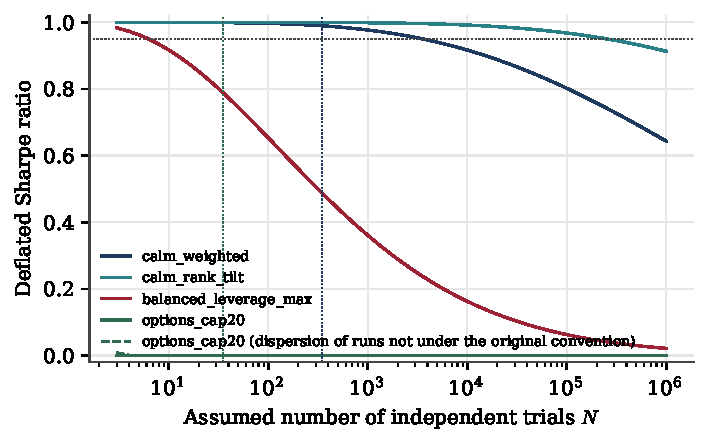
\includegraphics[width=0.75\linewidth]{figures/fig_dsr.pdf}
\caption{Deflated Sharpe ratio against the assumed number of trials. Dotted verticals mark the counted $N$ for equity and for options; the dashed green line recomputes the options curve with the dispersion of the runs not under the original convention only.}\label{fig:dsr}
\end{figure}

\subsection{Audit log: defects found}\label{sec:auditlog}

Table~\ref{tab:audit} lists every defect found, with before and after numbers where the saved results allow it, and Table~\ref{tab:ladder} and Figure~\ref{fig:ladder} attribute the correction of the four most recent defects fix by fix. The \emph{direction} of each correction shows how
fragile each headline number was: every correction applied to the saved runs lowered the reported return of most books, except that the corrected hold-period estimation raised returns for \stv{ladder.n_fix4_raise} of \stv{ladder.n_books} books (a noise-level effect: the search-window estimate was not worse) and that the
correction to the Sharpe denominator raised Sharpe ratios.

\begin{table}[t]\centering
\caption{Defects found. ``Before $\to$ after'' is return / Sharpe ratio where \texttt{results/} (or the ladder) contains both runs.}\label{tab:audit}
\small
\begin{tabularx}{\linewidth}{@{}p{2.6cm}X p{4.8cm}@{}}
\toprule
Defect & What exposed it & Effect (before $\to$ after)\\
\midrule
Look-ahead in the surprise deciles & Each surprise was ranked within its announcement quarter, i.e.\ against firms that had not reported yet; now ranked against the expanding pool of strictly earlier quarters, so the first quarter (\stv{pit.dropped} events) is dropped & \sn{calm_weighted}: \stv{ladder.calm_weighted.fix1.ret} / \stv{ladder.calm_weighted.fix1.sharpe} $\to$ \stv{ladder.calm_weighted.fix12.ret} / \stv{ladder.calm_weighted.fix12.sharpe}; median over \stv{ladder.n_books} equity books \stv{ladder.med.fix2} a year; 60-day signal spread \stv{pre.spread.mkt.h60} $\to$ \stv{spread.mkt.h60}\\
Leverage cap ignored open positions & The cap bounded only each quarter's new positions, so realized gross exposure ran above the stated cap; the cap now bounds the whole open book at sizing time & \sn{balanced_leverage_max}: \stv{ladder.balanced_leverage_max.published.ret} / \stv{ladder.balanced_leverage_max.published.sharpe} $\to$ \stv{ladder.balanced_leverage_max.fix1.ret} / \stv{ladder.balanced_leverage_max.fix1.sharpe}; median \stv{ladder.med.fix1} a year; days over the cap \stv{balanced_leverage_max_legacy.days_over_cap} $\to$ \stv{balanced_leverage_max.days_over_cap}\\
Mid-price option fills & Options were bought and sold at the mid with a flat percentage cost; the book pays the ask and receives the bid & 20\% book: \stv{ladder.options_cap20.published.ret} / \stv{ladder.options_cap20.published.sharpe} $\to$ \stv{ladder.options_cap20.fix3_only_bidask.ret} / \stv{ladder.options_cap20.fix3_only_bidask.sharpe} (bid/ask fills only)\\
Full-sample hold-period fitting & Decay days were estimated on the same history they were tested on; now estimated on the first \stv{fix.decay.pct} of announcement quarters (\stv{fix.decay.n} of \stv{fix.decay.of}) & \sn{calm_weighted}: \stv{ladder.calm_weighted.fix12.ret} $\to$ \stv{ladder.calm_weighted.all.ret}; median \stv{ladder.med.fix4} a year\\
Options quotes carried forward & Dead options (zero bid) were marked at their last live mid & 20\% book: \stv{optchain.legacy.ret} / \stv{optchain.legacy.sh} $\to$ \stv{optchain.floor.ret} / \stv{optchain.floor.sh} (before the fill fix)\\
Benchmark sensitivity of the long/short split & The all-announcer benchmark is biased when side and size are mixed, and it made the short leg look as good as the long leg & Long-to-short ratio \stv{sent.legs_all} (all-announcer) $\to$ \stv{ls.ratio.min} to \stv{ls.ratio.max} (size-matched)\\
Sharpe denominator & Daily P\&L was once divided by initial capital instead of prior-day NAV, overstating volatility as the NAV compounded & \sn{calm_weighted}: \stv{calm_weighted.sharpe_fixed} (fixed capital) $\to$ \ssh{calm_weighted}\\
EAR leakage & The day-0-to-day-1 return overlaps the first day of held P\&L; the Sharpe ratio rose with the weight on it & Sharpe ratio flat once removed; EAR not adopted (project history)\\
Ambient beta in the return law & The selector chose calls even in D1, since 1996--2013 was a net up market & Return law built from market-adjusted returns, recentered on a trailing drift (project history)\\
Strike units & OptionMetrics strikes were stored $\times1000$, so puts dominated even D10 at near-full Kelly fractions & Strikes divided by 1000 at source (project history)\\
Full-sample return law & Early trades were priced with later data & Walk-forward law after a \stv{kelly.warmup}-quarter warm-up\\
Independent Kelly sizing & The premium budget was exhausted by a few bets, which funded only a handful of positions & Kelly-proportional allocation of a shared budget (project history)\\
Per-cohort premium cap & Open premium could exceed the cap across overlapping 60-day cohorts & Cap on total outstanding premium (project history)\\
Data drift on a staged copy & Decay-day cells changed with no code change when a staged data copy was used & Results restored to the canonical data; checksum manifest and a pre-commit hook; the build pins pandas 3\\
\bottomrule
\end{tabularx}
\end{table}

The first seven rows trace to files in this repository (the saved runs, their legacy twins, and the ladder). The remaining rows were found and fixed before the saved runs; their before/after numbers predate \texttt{results/}, so we state the direction of the effect and not a number.

\begin{table}[t]\centering
\caption{Attribution ladder for selected equity books: annualized return as each fix is applied in turn (open-book cap, then point-in-time deciles, then search-window decay days), with the Sharpe ratio and maximum drawdown before and after all fixes. The full list is in Table~\ref{tab:ladderall}. ``Published'' is reproduced exactly by the saved \texttt{*\_legacy} runs.
Source: \texttt{docs/paper/cache/ladders/equity\_ladder.csv} (copied from the fixes work; see \texttt{docs/FIXES.md}).}\label{tab:ladder}
{\small
\begin{adjustbox}{max width=\linewidth}
\begin{tabular}{lrrrrrr}
\toprule
Book & Published & + cap & + deciles & + decay days & Sharpe & Max DD \\
\midrule
\sn{balanced_leverage} & 6.5\% & 6.4\% & 5.1\% & 5.4\% & 1.30 $\to$ 1.09 & $-$16.6\% $\to$ $-$18.6\% \\
\sn{calm_weighted} & 6.7\% & 6.6\% & 5.4\% & 5.6\% & 1.47 $\to$ 1.24 & $-$15.6\% $\to$ $-$17.5\% \\
\sn{calm_rank_tilt} & 7.1\% & 7.1\% & 5.8\% & 6.0\% & 1.81 $\to$ 1.47 & $-$11.6\% $\to$ $-$13.6\% \\
\sn{extreme_picks} & 4.9\% & 4.3\% & 2.8\% & 3.3\% & 0.93 $\to$ 0.65 & $-$18.5\% $\to$ $-$25.2\% \\
\sn{balanced_leverage_max} & 12.1\% & 10.3\% & 7.6\% & 8.3\% & 1.00 $\to$ 0.69 & $-$36.5\% $\to$ $-$44.9\% \\
\sn{market_boost} & 10.1\% & 10.0\% & 9.0\% & 9.2\% & 0.97 $\to$ 0.90 & $-$23.2\% $\to$ $-$25.1\% \\
\sn{market_boost_max} & 15.0\% & 13.5\% & 11.0\% & 11.6\% & 1.09 $\to$ 0.86 & $-$37.0\% $\to$ $-$44.6\% \\
\bottomrule
\end{tabular}
\end{adjustbox}
}

\end{table}

\begin{figure}[t]\centering
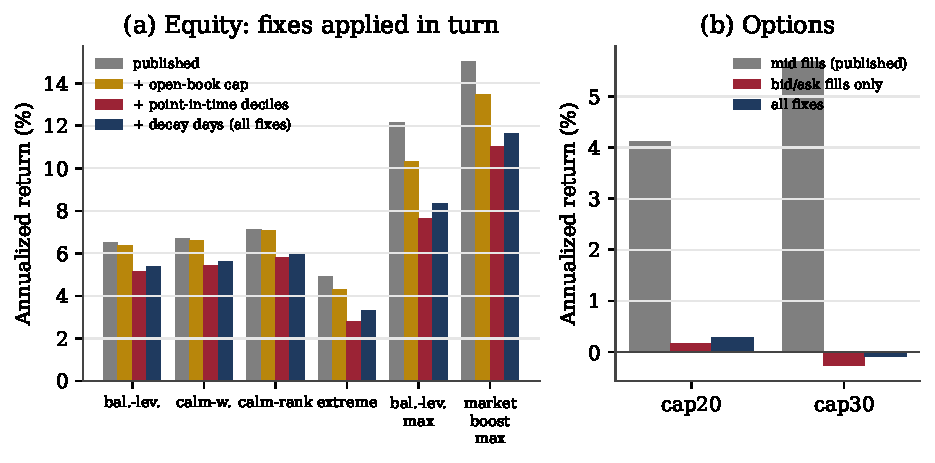
\includegraphics[width=\linewidth]{figures/fig_ladder.pdf}
\caption{The fix-attribution ladder. (a) Equity: annualized return as each fix is applied in turn. (b) Options: published (mid fills), bid/ask fills only, and all fixes.}\label{fig:ladder}
\end{figure}

Across the \stv{ladder.n_books} equity books, \stv{sent.biggest_fix}. The point-in-time deciles are the largest step for \stv{ladder.n_fix2_largest} books; the open-book cap (median step \stv{ladder.med.fix1}, range \stv{ladder.min.fix1} to \stv{ladder.max.fix1} points); the corrected
hold periods raise returns for \stv{ladder.n_fix4_raise} books (median \stv{ladder.med.fix4}). Taken together the corrections change return by a median of \stv{ladder.med.total} a year, and lower the Sharpe ratio for \stv{ladder.n_sharpe_lower} of \stv{ladder.n_books} books. The corrected caps hold at sizing time but gross exposure over the current NAV can still
exceed the cap when NAV falls (for \sn{balanced_leverage_max}, a peak of \stv{balanced_leverage_max.gross_max}$\times$ against a cap of \stv{balanced_leverage_max.cap}$\times$). \stv{sent.sweepnote}

\paragraph{What the corrections did not address.} \texttt{docs/FIXES.md} records the residual issues, which this paper inherits. The constants chosen on the full sample (the \sn{conviction_tilt} trim and tilt, the \sn{*_max} base-unit multipliers, the \sn{calm_weighted} unit, the \sn{calm_rank_tilt} exponent,
the blend weights) were deliberately not re-selected, so the corrected numbers remain partly in-sample and would most likely fall further if they were. The back-off thresholds of the hold-period cells and the leave-one-out risk benchmark still see the full sample; the weight normalisation uses quarter-wide
group totals that include later reporters; about a quarter of positions overlap the same stock's next event and the volume cap is not aggregated across overlapping positions; the Kelly selector scores at the mid but pays the ask; survivorship and delisting handling are unknown; and the expanding-pool ranking cannot absorb
market-wide surprise regimes, so decile sizes are uneven by quarter.

\begin{table}[t]\centering
\caption{Attribution ladder, all equity books (return as each fix is applied; Sharpe and drawdown before and after).}\label{tab:ladderall}
{\footnotesize
\begin{adjustbox}{max width=\linewidth}
\begin{tabular}{lrrrrrr}
\toprule
Book & Published & + cap & + deciles & + decay days & Sharpe & Max DD \\
\midrule
\sn{balanced_leverage} & 6.5\% & 6.4\% & 5.1\% & 5.4\% & 1.30 $\to$ 1.09 & $-$16.6\% $\to$ $-$18.6\% \\
\sn{balanced_leverage_max} & 12.1\% & 10.3\% & 7.6\% & 8.3\% & 1.00 $\to$ 0.69 & $-$36.5\% $\to$ $-$44.9\% \\
\sn{calm_rank_levered} & 9.2\% & 9.2\% & 7.6\% & 8.1\% & 1.73 $\to$ 1.39 & $-$15.9\% $\to$ $-$19.6\% \\
\sn{calm_rank_tilt} & 7.1\% & 7.1\% & 5.8\% & 6.0\% & 1.81 $\to$ 1.47 & $-$11.6\% $\to$ $-$13.6\% \\
\sn{calm_weighted} & 6.7\% & 6.6\% & 5.4\% & 5.6\% & 1.47 $\to$ 1.24 & $-$15.6\% $\to$ $-$17.5\% \\
\sn{calm_weighted_filter} & 6.5\% & 6.4\% & 5.1\% & 5.1\% & 1.41 $\to$ 1.08 & $-$15.7\% $\to$ $-$17.6\% \\
\sn{calm_weighted_matched} & 7.3\% & 6.7\% & 5.4\% & 5.8\% & 1.45 $\to$ 1.18 & $-$17.0\% $\to$ $-$18.7\% \\
\sn{conviction_tilt} & 5.2\% & 4.7\% & 3.7\% & 3.8\% & 1.18 $\to$ 0.97 & $-$13.1\% $\to$ $-$14.5\% \\
\sn{conviction_tilt_max} & 10.7\% & 10.7\% & 8.7\% & 9.3\% & 0.89 $\to$ 0.76 & $-$40.0\% $\to$ $-$40.5\% \\
\sn{extreme_picks} & 4.9\% & 4.3\% & 2.8\% & 3.3\% & 0.93 $\to$ 0.65 & $-$18.5\% $\to$ $-$25.2\% \\
\sn{extreme_picks_max} & 9.5\% & 9.5\% & 8.2\% & 9.0\% & 0.80 $\to$ 0.63 & $-$36.2\% $\to$ $-$56.4\% \\
\sn{graded_bets} & 3.9\% & 3.3\% & 2.0\% & 2.4\% & 1.01 $\to$ 0.62 & $-$14.0\% $\to$ $-$19.5\% \\
\sn{graded_bets_max} & 10.8\% & 10.4\% & 7.2\% & 8.6\% & 0.89 $\to$ 0.64 & $-$38.8\% $\to$ $-$48.0\% \\
\sn{market_boost} & 10.1\% & 10.0\% & 9.0\% & 9.2\% & 0.97 $\to$ 0.90 & $-$23.2\% $\to$ $-$25.1\% \\
\sn{market_boost_max} & 15.0\% & 13.5\% & 11.0\% & 11.6\% & 1.09 $\to$ 0.86 & $-$37.0\% $\to$ $-$44.6\% \\
\sn{market_exposed} & 7.3\% & 7.2\% & 5.6\% & 6.6\% & 1.11 $\to$ 0.72 & $-$15.5\% $\to$ $-$34.1\% \\
\sn{market_exposed_max} & 11.8\% & 11.8\% & 10.0\% & 11.5\% & 1.00 $\to$ 0.72 & $-$33.0\% $\to$ $-$53.8\% \\
\sn{sector_balanced} & 4.1\% & 4.0\% & 3.1\% & 3.1\% & 1.33 $\to$ 1.08 & $-$10.8\% $\to$ $-$11.4\% \\
\sn{sector_balanced_max} & 12.1\% & 10.3\% & 7.6\% & 8.3\% & 1.00 $\to$ 0.69 & $-$36.5\% $\to$ $-$44.9\% \\
\sn{size_balanced} & 4.7\% & 4.3\% & 3.3\% & 3.8\% & 0.91 $\to$ 0.81 & $-$17.5\% $\to$ $-$18.1\% \\
\sn{size_balanced_max} & 8.4\% & 8.4\% & 8.1\% & 8.9\% & 0.72 $\to$ 0.72 & $-$37.5\% $\to$ $-$43.6\% \\
\sn{volatility_filter} & 6.3\% & 6.1\% & 4.7\% & 4.6\% & 1.23 $\to$ 0.89 & $-$16.7\% $\to$ $-$18.8\% \\
\bottomrule
\end{tabular}
\end{adjustbox}
}

\end{table}
No equity book has a legacy twin in \texttt{results/} yet, so no before/after comparison of the three equity corrections can be produced from the saved runs.

\begin{table}[t]\centering
\caption{Effect of the equity corrections on every book that has a saved pre-correction twin.}\label{tab:twins}
{\small
\begin{adjustbox}{max width=\linewidth}
\begin{tabular}{lrrrrrr}
\toprule
 & \multicolumn{3}{c}{Before the fix (legacy twin)} & \multicolumn{3}{c}{After the fix}\\
\cmidrule(lr){2-4}\cmidrule(lr){5-7}
Book & Return & Sharpe & Max DD & Return & Sharpe & Max DD \\
\midrule
\sn{balanced_leverage} & 6.5\% & 1.30 & $-$16.6\% & 5.4\% & 1.09 & $-$18.6\% \\
\sn{balanced_leverage_max} & 12.1\% & 1.00 & $-$36.5\% & 8.3\% & 0.69 & $-$44.9\% \\
\sn{calm_rank_levered} & 9.2\% & 1.73 & $-$15.9\% & 8.1\% & 1.39 & $-$19.6\% \\
\sn{calm_rank_tilt} & 7.1\% & 1.81 & $-$11.6\% & 6.0\% & 1.47 & $-$13.6\% \\
\sn{calm_weighted_filter} & 6.5\% & 1.41 & $-$15.7\% & 5.1\% & 1.08 & $-$17.6\% \\
\sn{calm_weighted} & 6.7\% & 1.47 & $-$15.6\% & 5.6\% & 1.24 & $-$17.5\% \\
\sn{calm_weighted_matched} & 7.3\% & 1.45 & $-$17.0\% & 5.8\% & 1.18 & $-$18.7\% \\
\sn{conviction_tilt} & 5.2\% & 1.18 & $-$13.1\% & 3.8\% & 0.97 & $-$14.5\% \\
\sn{conviction_tilt_max} & 10.7\% & 0.89 & $-$40.0\% & 9.3\% & 0.76 & $-$40.5\% \\
\sn{extreme_picks} & 4.9\% & 0.93 & $-$18.5\% & 3.3\% & 0.65 & $-$25.2\% \\
\sn{extreme_picks_max} & 9.5\% & 0.80 & $-$36.2\% & 9.0\% & 0.63 & $-$56.4\% \\
\sn{graded_bets} & 3.9\% & 1.01 & $-$14.0\% & 2.4\% & 0.62 & $-$19.5\% \\
\sn{graded_bets_max} & 10.8\% & 0.89 & $-$38.8\% & 8.6\% & 0.64 & $-$48.0\% \\
\sn{market_boost} & 10.1\% & 0.97 & $-$23.2\% & 9.2\% & 0.90 & $-$25.1\% \\
\sn{market_boost_max} & 15.0\% & 1.09 & $-$37.0\% & 11.6\% & 0.86 & $-$44.6\% \\
\sn{market_exposed} & 7.3\% & 1.11 & $-$15.5\% & 6.6\% & 0.72 & $-$34.1\% \\
\sn{market_exposed_max} & 11.8\% & 1.00 & $-$33.0\% & 11.5\% & 0.72 & $-$53.8\% \\
\sn{sector_balanced} & 4.1\% & 1.33 & $-$10.8\% & 3.1\% & 1.08 & $-$11.4\% \\
\sn{sector_balanced_max} & 12.1\% & 1.00 & $-$36.5\% & 8.3\% & 0.69 & $-$44.9\% \\
\sn{size_balanced} & 4.7\% & 0.91 & $-$17.5\% & 3.8\% & 0.81 & $-$18.1\% \\
\sn{size_balanced_max} & 8.4\% & 0.72 & $-$37.5\% & 8.9\% & 0.72 & $-$43.6\% \\
\sn{volatility_filter} & 6.3\% & 1.23 & $-$16.7\% & 4.6\% & 0.89 & $-$18.8\% \\
\bottomrule
\end{tabular}
\end{adjustbox}
}
\end{table}



%=====================================================================================
\section{Limitations and what is not modelled}\label{sec:limits}
%=====================================================================================

We list these without softening. Each is either a reason realized performance would be lower or a test still to be run.
\begin{enumerate}
\item \textbf{The corrections lowered the headline numbers, and what remains is still partly in-sample.} The corrected returns are in Table~\ref{tab:ladder}. The constants chosen on the full sample before the corrections (trim, tilt, base units and the six-times ceiling, the
      \sn{calm_rank_tilt} exponent, option caps, blend multiples) were not re-selected. Re-selecting them on a search window is an open task and would most likely lower the figures further. The split-sample check of Section~\ref{sec:eqresults} predates the corrections and was not re-run.
\item \textbf{Sample period and decay.} All results are for 1996--2013, and alpha per dollar was lower in the last era in \stv{era.all.fade.n} of nine profiled books (to between \stv{era.all.CA.min} and \stv{era.all.CA.max} of its first-era level). A data extension and a post-publication
      decay adjustment \citep{McLeanPontiff2016} are required before any capital is allocated.
\item \textbf{Residual look-ahead.} The corrections remove the decile look-ahead and the full-sample decay-day fit, not every use of future information: the hold-period back-off thresholds, the leave-one-out risk benchmark and the weight normalisation still see the full sample, and the
      signal tables of Sections~\ref{sec:data}--\ref{sec:evidence} that depend on the option chain or on volatility terciles (option spreads, the volatility diagnostic) were not rebuilt on point-in-time deciles.
\item \textbf{Borrow fees and financing (equity).} Neither is modelled, and the short leg is small-cap-heavy. The short side averages \stv{calm_weighted.short_avg}$\times$ NAV for \sn{calm_weighted}, so each 1\% a year of borrow cost removes \stv{calm_weighted.borrow_1pct} of
      return; a fee of \stv{calm_weighted.borrow_breakeven} would remove all of it, and a uniform 5\% would leave \stv{calm_weighted.ret_at5} (for \sn{balanced_leverage}: \stv{balanced_leverage.ret_at5}). Hard-to-borrow names cost more, and the model of
      Section~\ref{sec:mechanism} predicts they are the names with the most drift. Gross exposure above NAV and the stacked blend multiples also need financing.
\item \textbf{Market impact and capacity (equity).} The \stv{balanced_leverage_max.liqfrac} volume cap is a participation limit, not an impact model. \stv{calm_weighted.liqcap} of \sn{calm_weighted}'s positions and \stv{balanced_leverage_max.liqcap} of \sn{balanced_leverage_max}'s sit at the cap
      \citep{FrazziniIsraelMoskowitz2018,NovyMarxVelikov2016}. Costs are \stv{cost.min}--\stv{cost.max} basis points per side by liquidity quintile.
\item \textbf{Leverage and the drawdown screen.} The cap now bounds the open book at sizing time, but gross exposure over current NAV can exceed it, and the \sn{*_max} books run at several times NAV. \stv{max.n_breach} of the \stv{max.n} \sn{*_max} books now breach the
      drawdown limit ($-$\stv{rule.dd}) that was used to choose their size, with a worst drawdown of \stv{max.worst_dd}; they are research variants and are not presented as achievable results.
\item \textbf{Option execution.} The book now pays the quoted ask and receives the quoted bid, which removed the measured edge; the selector still scores at the mid, there is no market impact, and the book opens about \stv{options_cap20.pos_per_year} positions a year.
\item \textbf{Options data coverage.} 2011 is missing because its source file is structurally corrupt, so the trading-day calendar compresses across the gap, and 2013 ends in August. The matched sample is tilted toward names with liquid, longer-dated chains.
\item \textbf{Return-law pooling.} One distribution per (decile, quarter) is shared by every stock in the decile, regardless of its own volatility.
\item \textbf{Live universe.} The backtest trades the full CRSP event universe. A live book restricted to large stocks earns much less per dollar: for \sn{balanced_leverage}, \stv{sit.small.b} basis points in the largest company-size quintile against \stv{sit.small.a} in the smallest.
\item \textbf{Reporting convention.} Stored summary statistics cover each book's full calendar, including idle periods before the first position; the active-period figures differ slightly (Section~\ref{sec:engine}). The equity daily series runs to \stv{calendar_end}
      while events end in 2013.
\item \textbf{What the earlier drafts claimed that is not repeated.} The earlier drafts quoted an equity book at \stv{olddraft.eq.ret} as the strategy, an options book at \sret{options_cap30_legacy} and a Sharpe ratio of \ssh{options_cap30_legacy}, and a blend at
      \stv{hedged_blend_prefix_fix.ret}. None of these is a result here.
\end{enumerate}


%=====================================================================================
\section{Conclusion}\label{sec:conclusion}
%=====================================================================================

Post-earnings-announcement drift is present in this sample, and it survives the corrections: the 60-day top-minus-bottom spread with point-in-time deciles is \stv{spread.mkt.h60} (\stv{pre.spread.mkt.h60} with the within-quarter ranking), it is significant under earnings-season clustering, it survives
a size/value characteristic benchmark (which \stv{sent.ffvsmkt} the spread), its spread \stv{sent.sizemono} with firm size, as limits to arbitrage predict, and it appears in option premia measured at mid prices.

What it is worth as a strategy is smaller than earlier drafts reported. The market-neutral equity books earn \sret{calm_weighted} (\sn{calm_weighted}, Sharpe \ssh{calm_weighted}) and, for the research book with an in-sample exponent, \sret{calm_rank_tilt} (\sn{calm_rank_tilt}, Sharpe \ssh{calm_rank_tilt}), against
\stv{calm_weighted_legacy.ret} and \stv{calm_rank_tilt_legacy.ret} before the corrections; \stv{sent.biggest_fix}. The options book, which earlier drafts credited with an edge and a diversifying role, earns \sret{options_cap20} at a Sharpe ratio of \ssh{options_cap20} when it is filled at the ask and the bid; it \stv{sent.opt_edge}, and the previously reported edge
was largely an artifact of mid-price fills. The blends fall accordingly: \sn{hedged_blend} earns \sret{hedged_blend} (Sharpe \ssh{hedged_blend}) and has \stv{sent.blend_vs_equity}. The levered \sn{*_max} books and the market-exposed variants earn more only by taking more risk, and
\stv{max.n_breach} of \stv{max.n} \sn{*_max} books now breach the drawdown screen used to size them; \sn{market_boost} \stv{sent.mb_clears} the market's \stv{market.ret} over the same calendar.

The decomposition adds cautions that the headline numbers hide. The most profitable recipe is the same in \stv{best.n_top} of nine books (a long position in a thinly traded, low-beta stock held more than two months). \stv{sent.hbs}. In the beta-by-volatility cut the larger margin is \stv{sent.bv.larger}. Against a size-matched benchmark
\stv{sent.legs}; alpha per dollar was \stv{eraA.bp} basis points in 1996--2001 and \stv{eraC.bp} in 2008--13 for \sn{balanced_leverage}. The mechanism of Section~\ref{sec:mechanism} adds that the places where the drift is largest are the places where the costs we do not model are largest.
The work that remains before deployment is concrete: re-select the in-sample constants on a search window, remove the residual look-ahead listed in Section~\ref{sec:auditlog}, add borrow, financing and impact costs, score options at the price they will pay, and extend the data beyond 2013.

\vspace{1em}
\noindent\fbox{\parbox{\dimexpr\linewidth-2\fboxsep-2\fboxrule}{\footnotesize
\textbf{Disclosure.} All performance figures are hypothetical, are based on historical backtests (1996--2013) net of modeled trading costs, and do not reflect actual trading. They benefit from hindsight in
model design, and the modeling assumptions in Section~\ref{sec:limits} omit costs that would lower them. Realized results may differ materially. Nothing here is an offer, a solicitation, or investment advice.}}

%=====================================================================================
\appendix
\section{Names used in earlier drafts and here}\label{app:names}
%=====================================================================================

\begin{table}[h]\centering
\caption{Mapping from the numbered labels used in earlier drafts and the project history to the plain names used in this paper. The rename retired the numbered labels and left every number unchanged. Result folders carry suffixes: \texttt{\_legacy} is the pre-correction run of an equity book, \texttt{\_prefix\_fix} the pre-correction run of an options book or blend, \texttt{\_midfill} an options book with mid fills on the corrected deciles.}\label{tab:oldnames}
{\small
\begin{tabularx}{\linewidth}{@{}p{0.43\linewidth}X@{}}
\toprule
Label in earlier drafts & Plain name here\\
\midrule
Strategy 1 (extreme-decile L/S) & \sn{extreme_picks} \\
Strategy 2 (rank-weighted) & \sn{graded_bets} \\
Strategy 3 (balanced) & \sn{size_balanced} \\
Strategy 4 & \sn{conviction_tilt} \\
Strategy 5 & \sn{sector_balanced} \\
Strategy 6 & \sn{balanced_leverage} \\
Strategy 6 + 0.5x beta overlay & \sn{market_boost} \\
Strategy 7 & \sn{market_exposed} \\
Strategy 9a & \sn{volatility_filter} \\
Strategy 9b & \sn{calm_weighted} \\
Strategy 9c & \sn{calm_weighted_filter} \\
Strategy 10 & \sn{calm_rank_tilt} \\
Strategy 6 / 5 / 4 ... Aggressive & balanced\_leverage\_max, sector\_balanced\_max, ... (the *\_max books) \\
Strategy I (earlier drafts' equity headline) & balanced\_leverage\_max (= sector\_balanced\_max) \\
Strategy II, opt\_kelly\_cap30 (earlier drafts' options headline) & options\_cap30\_legacy (overstated); corrected: options\_cap30 \\
opt\_kelly\_cap20 & options\_cap20\_legacy (overstated); corrected: options\_cap20 \\
opt\_kelly\_cap40 & \sn{options_cap40_legacy} \\
Strategy 8 (walk-forward ML) & not in the framework; excluded (ran on an unverified data copy) \\
\bottomrule
\end{tabularx}
}

\end{table}

%=====================================================================================
\section{Parameters and reproducibility}\label{app:repro}
%=====================================================================================

\begin{table}[h]\centering
\caption{Equity parameters (from each run's \texttt{summary.json}). Base unit is the fraction of trailing NAV per unit of weight; the gross cap applies per entry cohort.}\label{tab:paramseq}
{\small
\begin{adjustbox}{max width=\linewidth}
\begin{tabular}{lrrrllll}
\toprule
Book & Base unit & Gross cap & ADV cap & Returns & Trim rule & Cap on & Overlay \\
\midrule
\sn{extreme_picks} & 0.003 & 1.5$\times$ & 5\% & mktadj & proportional & open\_book & 0 \\
\sn{graded_bets} & 0.002 & 1.5$\times$ & 5\% & mktadj & proportional & open\_book & 0 \\
\sn{size_balanced} & 0.003 & 1.5$\times$ & 5\% & mktadj & proportional & open\_book & 0 \\
\sn{conviction_tilt} & 0.002 & 1.5$\times$ & 5\% & mktadj & priority & open\_book & 0 \\
\sn{sector_balanced} & 0.0015 & 1.5$\times$ & 5\% & mktadj & priority & open\_book & 0 \\
\sn{balanced_leverage} & 0.003 & 2.5$\times$ & 5\% & mktadj & priority & open\_book & 0 \\
\sn{market_boost} & 0.003 & 2.5$\times$ & 5\% & mktadj & priority & open\_book & 0.5 \\
\sn{market_exposed} & 0.003 & 2.5$\times$ & 5\% & raw & priority & open\_book & 0 \\
\sn{calm_weighted} & 0.003 & 2.5$\times$ & 5\% & mktadj & priority & open\_book & 0 \\
\sn{calm_rank_tilt} & 0.003 & 2.5$\times$ & 5\% & mktadj & priority & open\_book & 0 \\
\sn{calm_rank_levered} & 0.005 & 4$\times$ & 5\% & mktadj & priority & open\_book & 0 \\
\sn{balanced_leverage_max} & 0.012 & 6$\times$ & 5\% & mktadj & priority & open\_book & 0 \\
\sn{market_boost_max} & 0.012 & 6$\times$ & 5\% & mktadj & priority & open\_book & 0.5 \\
\bottomrule
\end{tabular}
\end{adjustbox}
}

\end{table}
\begin{table}[h]\centering
\caption{Options parameters (from each run's \texttt{summary.json}).}\label{tab:paramsop}
{\small
\begin{adjustbox}{max width=\linewidth}
\begin{tabular}{lrrrrrl}
\toprule
Book & Premium cap & Kelly mult. & Hold (d) & Round-trip & Floor / share & Dead-quote mark \\
\midrule
\sn{options_cap20} & 0.2 & 0.5 & 60 & 3\% & \$0.05 & zero\_bid\_half\_ask \\
\sn{options_cap30} & 0.3 & 0.5 & 60 & 3\% & \$0.05 & zero\_bid\_half\_ask \\
\sn{options_worst_case} & 0.2 & 0.5 & 60 & 3\% & \$0.05 & zero\_bid\_zero \\
\sn{options_cap20_legacy} & 0.2 & 0.5 & 60 & 3\% & \$0.00 & carry\_last \\
\sn{options_cap30_legacy} & 0.3 & 0.5 & 60 & 3\% & \$0.00 & carry\_last \\
\sn{options_cap40_legacy} & 0.4 & 0.5 & 60 & 3\% & \$0.00 & carry\_last \\
\bottomrule
\end{tabular}
\end{adjustbox}
}

\end{table}

\paragraph{Weights.} Trim $\tau=\stv{balanced_leverage.trim}$ and tilt $\gamma=\stv{balanced_leverage.tilt}$; groups are (side, size quintile, Fama--French industry) within each announcement quarter; the weights are rescaled to a mean absolute value of $0.5$.
\paragraph{Holding windows.} Per-cell decay days (Section~\ref{sec:decay}), from \stv{decay.min} to \stv{decay.max} trading days.
\paragraph{Runs.} The \stv{n_runs} saved runs in \texttt{results/} were produced between \stv{runs.first} and \stv{runs.last} at git revision(s) \stv{runs.revs} under pandas \stv{runs.pandas}; results reproduce only under the pinned pandas 3 (see \texttt{requirements.txt}). \texttt{results/<name>} holds the run with all four corrections of \texttt{docs/FIXES.md}; \texttt{*\_legacy} (equity) and \texttt{*\_prefix\_fix} (options, blends) keep the pre-correction numbers, and \texttt{*\_midfill} the mid-fill options references.

\paragraph{Data vintages.} The committed \texttt{data/} tables are the pre-correction vintage (within-quarter deciles). The corrected vintage was built in an isolated directory (\texttt{PEAD\_FIXED\_DATA}, default \texttt{../vintage\_fixed/data} beside the worktree) and is not committed. From it the builder recomputes the point-in-time decile tables and subsample spreads (Fama--MacBeth means, validated by reproducing the committed tables exactly from the old event file) and copies the size/book-to-market tables and the decay-day table into \texttt{docs/paper/cache/pit/}. The attribution ladders are copied from the fixes work into \texttt{docs/paper/cache/ladders/} with a provenance note. The option-spread tables, the volatility diagnostic and the SUE-reversal summary exist only in the pre-correction vintage and are labelled as such.

\paragraph{Where every number comes from.}\begin{sloppypar}
Per-book statistics: \texttt{results/<name>/summary.json} and \texttt{daily.csv.gz} (realized leverage, active-period Sharpe, calendar returns, correlations, deflated Sharpe ratios). Leaderboard checks: \texttt{results/leaderboard.json} and \texttt{leaderboard.md}.
Alpha against the market: \texttt{results/alpha\_benchmark.csv}. Situations: \texttt{results/situations\_*.csv}. Recipes, leg and beta splits, timing and tails: \texttt{results/profiles\_*.csv}. Capital-split frontier: \texttt{results/portfolio/frontier.csv}.
Signal evidence (Sections~\ref{sec:data}--\ref{sec:evidence}): the committed tables under \texttt{data/} (\texttt{decile\_horizon\_stats}, \texttt{spread\_horizon\_stats}, the \texttt{ff\_*} and \texttt{option\_*} versions, \texttt{subsample\_*}, \texttt{sue\_reversal\_summary.json}, \texttt{cell\_decay\_days.csv},
\texttt{vol\_decile\_diagnostic\_summary.json}), plus \texttt{data/sweep\_*.csv} and the options comparison files for the trial count and the capacity table. Construction constants (trim, tilt, exponent, costs, grids) are read from the strategy classes and engine modules.
Four groups of numbers need files that are not committed: the $3\times3$ beta-by-volatility cut and the per-trade options statistics (from \texttt{results/*/positions.parquet}, git-ignored), the point-in-time signal tables (corrected event file) and the CRSP market series (licensed). They are recomputed whenever the main repository's data is reachable (environment variable
\texttt{PEAD\_MAIN\_REPO}) and the run it holds is the run in \texttt{results/}; otherwise the committed cache in \texttt{docs/paper/cache/} is used, and the build warns when the cache is stale.

\end{sloppypar}
\paragraph{Rebuilding.} After any change to \texttt{results/} or \texttt{data/}, one command rebuilds the statistics, tables, figures and PDF with no hand edits:
\begin{center}\texttt{python -m pead.reporting.paper}\end{center}
(equivalently \texttt{python -m pead paper}; \texttt{--no-pdf} skips the LaTeX step, \texttt{--refresh-external} recomputes the cached quantities). The build fails if a number macro used here is undefined, if a strategy name used here is not in \texttt{results/}, if
\texttt{results/leaderboard.md} disagrees with the saved summaries, or if a numbered legacy label appears in the text.

\paragraph{Code.} Strategy files: \texttt{pead/strategies/}; engines: \texttt{pead/engines/}; reports and attribution: \texttt{pead/reporting/}; this paper: \texttt{pead/reporting/paper.py} and \texttt{paper\_figures.py}.

%=====================================================================================
\section{Proofs}\label{app:proofs}
%=====================================================================================

\paragraph{Concavity of the incorporation profile.}
A Gamma$(k,\theta)$ mixture of exponential rates has Laplace transform $\E[e^{-\kappa d}]=(1+d/\theta)^{-k}$, which gives \eqref{eq:phi}. Then
$\phi'(d)=(1-\phi(0))\,(k/\theta)\,(1+d/\theta)^{-k-1}>0$ and $\phi''(d)<0$, so $\phi$ is increasing and strictly concave with $\phi(d)\to1$. Since $\Delta(h)\propto\phi(h)-\phi(0)$, the spread is increasing, concave and
bounded. The unincorporated fraction decays as a power, $(1+d/\theta)^{-k}$, not exponentially, so the profile has no single time scale and keeps rising long after a single-speed model would have flattened.

\paragraph{Uniqueness of the holding period.}
Write $\mathcal Y(H)=(a(H)-k)/H$ with $a$ increasing and concave, $a(0)=0$, and $a(\infty)>k$. Then $\mathcal Y'(H)=N(H)/H^2$ with $N(H)=a'(H)H-a(H)+k$, and $N(H)=0$ if and only if $a'(H)=\mathcal Y(H)$. Now
$N'(H)=a''(H)H<0$, $N(0)=k>0$, and $N(H)\to k-a(\infty)<0$ as $H\to\infty$ (because $a'(H)H\to0$ for a concave bounded $a$). So $N$ has exactly one zero $H^\ast$, and $\mathcal Y$ increases before it and decreases after,
which makes $H^\ast$ the unique maximizer. $\square$

\paragraph{Proof of Proposition~\ref{prop:neutral}.}
Fix $q$ and side $\sigma$. For an occupied group $g$, $\sum_{i\in g}|\tilde w_i|=\sum_{i\in g}|t_i|\big/\big(\sum_{j\in g}|t_j|\cdot N_{q\sigma}\big)=1/N_{q\sigma}$, which proves (b); the per-event scale $s_i$ is inside $t_i$ and
cancels in this ratio, so it moves weight only within a group. Summing over the $N_{q\sigma}$ groups on a side gives $\sum_{i\in q\sigma}|\tilde w_i|=1$ for both sides. Every weight on a side has the same sign, so the long gross equals the short gross,
and the global rescaling in \eqref{eq:weights} multiplies all weights by one positive constant, which proves (a). For (c), industry $k$'s long gross is the sum over its occupied long groups, $n^+_k/N_{q+}$, and likewise on the short side.
Net exposure is the difference, and it vanishes when $n^{+}_{k}/N_{q+}=n^{-}_{k}/N_{q-}$, in particular when both sides occupy the same set of groups. The size argument is symmetric. $\square$

\paragraph{Proof of Proposition~\ref{prop:capacity}.}
Let the notional of position $i$ be $n_i=\min(|w_i|\,bV,\,\ell_i)$, where $\ell_i$ is its liquidity limit. Position $i$ stops absorbing marginal capital at $b_i=\ell_i/(|w_i|V)$, which increases in liquidity. Write
$\mathcal U(b)=\{i:b<b_i\}$ for the uncapped set, which shrinks as $b$ grows. The marginal alpha per marginal gross dollar is the $|w|$-weighted average of $\alpha_i$ over $\mathcal U(b)$. Raising $b$ removes the members with
the smallest $b_i$, which are the least liquid names and, by assumption, those with the largest $\alpha_i$. The weighted average therefore cannot increase, so expected arithmetic P\&L, the integral of this non-increasing
marginal alpha, is concave in $b$. Volatility is non-decreasing in gross exposure, so $\mu(b)-\tfrac12\sigma^2(b)$ is concave with $\mu(0)=\sigma(0)=0$ and positive slope at zero when the uncapped book has positive alpha.
As $b\to\infty$ the alpha saturates while the variance term does not, so the function eventually decreases and the maximum is interior. $\square$

\paragraph{Proof of Proposition~\ref{prop:wellposed}.}
$R_{k,s}\ge-1$ and $f\le\stv{kelly.fmax}$ give $1+fR_{k,s}\ge1-\stv{kelly.fmax}>0$. The second derivative is $G''_k(f)=-\sum_sp_sR_{k,s}^2/(1+fR_{k,s})^2<0$ unless every $R_{k,s}=0$. Direct evaluation gives
$G_k(0)=0$ and $G_k'(0)=\sum_sp_sR_{k,s}$. Since $G_k$ is concave, its maximizer on $[0,1)$ is positive if and only if $G_k'(0)>0$. $\square$

\paragraph{Proof of Proposition~\ref{prop:sharpe}.}
Substitute $\log(1+y)=y-\tfrac12y^2+O(y^3)$ and take expectations, which gives $G_k(f)=f\mu_k-\tfrac12f^2m_k+O(f^3\E|R_k|^3)$. Maximizing the quadratic gives $f^\ast=\mu_k/m_k$ and $g^\ast=\mu_k^2/(2m_k)$. Dividing numerator and
denominator by $\sigma_k^2$ gives $\tfrac12\mathrm{SR}_k^2/(1+\mathrm{SR}_k^2)$, which is increasing in $\mathrm{SR}_k$ for $\mathrm{SR}_k>0$. $\square$

\paragraph{Proof of Proposition~\ref{prop:hurdle}.}
$G_k$ is concave with $G_k(0)=0$. If $G_k(f_{\min})\le0$, concavity gives $G_k(f)\le(f/f_{\min})\,G_k(f_{\min})\le0$ for every $f\ge f_{\min}$, so no stake on the grid has positive growth and the contract cannot be selected.
Selectability therefore requires $G_k(f_{\min})>0$. In the quadratic approximation this reads $f_{\min}\mu_k-\tfrac12f_{\min}^2m_k>0$, which is \eqref{eq:hurdle}. $\square$

\paragraph{Proof of Proposition~\ref{prop:fractional}.}
(a) is immediate from \eqref{eq:alloc}. (b) Under independence and the quadratic approximation, portfolio growth is $\sum_i(\pi_i\mu_i-\tfrac12\pi_i^2m_i)$. Setting $\pi_i=\lambda\mu_i/m_i$ gives
$\sum_i\frac{\mu_i^2}{m_i}\big(\lambda-\tfrac12\lambda^2\big)=(2\lambda-\lambda^2)\sum_ig^\ast_i$. The portfolio mean is $\lambda\sum_i\mu_i^2/m_i$ and its standard deviation is
$\lambda(\sum_i\mu_i^2\sigma_i^2/m_i^2)^{1/2}$, so $\lambda$ cancels in the ratio. With $N$ bets of comparable size, the numerator is $O(N)$ and the denominator $O(\sqrt N)$. (c) A long option position costs its premium and has a
non-negative payoff, so its loss is at most the premium, and premium outstanding is at most $cV_q$ by construction of $B_q$. $\square$

%=====================================================================================
\begin{thebibliography}{99}\small
%=====================================================================================
\bibitem[Bailey and L\'opez de Prado(2012)]{BaileyLopezdePrado2012}
Bailey, D.~H., and M.~L\'opez de Prado (2012). The Sharpe ratio efficient frontier.
\textit{Journal of Risk} 15(2), 3--44.

\bibitem[Bailey and L\'opez de Prado(2014)]{BaileyLopezdePrado2014}
Bailey, D.~H., and M.~L\'opez de Prado (2014). The deflated Sharpe ratio: correcting for selection bias,
backtest overfitting, and non-normality. \textit{Journal of Portfolio Management} 40(5), 94--107.

\bibitem[Ball and Brown(1968)]{BallBrown1968}
Ball, R., and P.~Brown (1968). An empirical evaluation of accounting income numbers.
\textit{Journal of Accounting Research} 6(2), 159--178.

\bibitem[Bernard and Thomas(1989)]{BernardThomas1989}
Bernard, V.~L., and J.~K.~Thomas (1989). Post-earnings-announcement drift: delayed price
response or risk premium? \textit{Journal of Accounting Research} 27 (Supplement), 1--36.

\bibitem[Bernard and Thomas(1990)]{BernardThomas1990}
Bernard, V.~L., and J.~K.~Thomas (1990). Evidence that stock prices do not fully reflect
the implications of current earnings for future earnings. \textit{Journal of Accounting and
Economics} 13(4), 305--340.

\bibitem[Daniel et~al.(1997)]{DGTW1997}
Daniel, K., M.~Grinblatt, S.~Titman, and R.~Wermers (1997). Measuring mutual fund
performance with characteristic-based benchmarks. \textit{Journal of Finance} 52(3),
1035--1058.

\bibitem[Daniel and Moskowitz(2016)]{DanielMoskowitz2016}
Daniel, K., and T.~J.~Moskowitz (2016). Momentum crashes. \textit{Journal of Financial
Economics} 122(2), 221--247.

\bibitem[DellaVigna and Pollet(2009)]{DellaVignaPollet2009}
DellaVigna, S., and J.~M.~Pollet (2009). Investor inattention and Friday earnings
announcements. \textit{Journal of Finance} 64(2), 709--749.

\bibitem[Fama and MacBeth(1973)]{FamaMacBeth1973}
Fama, E.~F., and J.~D.~MacBeth (1973). Risk, return, and equilibrium: empirical tests.
\textit{Journal of Political Economy} 81(3), 607--636.

\bibitem[Frazzini et~al.(2018)]{FrazziniIsraelMoskowitz2018}
Frazzini, A., R.~Israel, and T.~J.~Moskowitz (2018). Trading costs. Working paper, AQR
Capital Management.

\bibitem[Grinold(1989)]{Grinold1989}
Grinold, R.~C. (1989). The fundamental law of active management. \textit{Journal of
Portfolio Management} 15(3), 30--37.

\bibitem[Hirshleifer et~al.(2009)]{HirshleiferLimTeoh2009}
Hirshleifer, D., S.~S.~Lim, and S.~H.~Teoh (2009). Driven to distraction: extraneous events
and underreaction to earnings news. \textit{Journal of Finance} 64(5), 2289--2325.

\bibitem[Hong and Stein(1999)]{HongStein1999}
Hong, H., and J.~C.~Stein (1999). A unified theory of underreaction, momentum trading, and
overreaction in asset markets. \textit{Journal of Finance} 54(6), 2143--2184.

\bibitem[Kelly(1956)]{Kelly1956}
Kelly, J.~L. (1956). A new interpretation of information rate. \textit{Bell System
Technical Journal} 35(4), 917--926.

\bibitem[MacLean et~al.(2011)]{MacLeanThorpZiemba2011}
MacLean, L.~C., E.~O.~Thorp, and W.~T.~Ziemba, eds. (2011). \textit{The Kelly Capital Growth
Investment Criterion: Theory and Practice}. World Scientific.

\bibitem[McLean and Pontiff(2016)]{McLeanPontiff2016}
McLean, R.~D., and J.~Pontiff (2016). Does academic research destroy stock return
predictability? \textit{Journal of Finance} 71(1), 5--32.

\bibitem[Mendenhall(2004)]{Mendenhall2004}
Mendenhall, R.~R. (2004). Arbitrage risk and post-earnings-announcement drift.
\textit{Journal of Business} 77(4), 875--894.

\bibitem[Novy-Marx and Velikov(2016)]{NovyMarxVelikov2016}
Novy-Marx, R., and M.~Velikov (2016). A taxonomy of anomalies and their trading costs.
\textit{Review of Financial Studies} 29(1), 104--147.

\bibitem[Shleifer and Vishny(1997)]{ShleiferVishny1997}
Shleifer, A., and R.~W.~Vishny (1997). The limits of arbitrage. \textit{Journal of
Finance} 52(1), 35--55.
\end{thebibliography}

\end{document}
